\documentclass[twoside]{book}

% Packages required by doxygen
\usepackage{fixltx2e}
\usepackage{calc}
\usepackage{doxygen}
\usepackage[export]{adjustbox} % also loads graphicx
\usepackage{graphicx}
\usepackage[utf8]{inputenc}
\usepackage{makeidx}
\usepackage{multicol}
\usepackage{multirow}
\PassOptionsToPackage{warn}{textcomp}
\usepackage{textcomp}
\usepackage[nointegrals]{wasysym}
\usepackage[table]{xcolor}

% Font selection
\usepackage[T1]{fontenc}
\usepackage[scaled=.90]{helvet}
\usepackage{courier}
\usepackage{amssymb}
\usepackage{sectsty}
\renewcommand{\familydefault}{\sfdefault}
\allsectionsfont{%
  \fontseries{bc}\selectfont%
  \color{darkgray}%
}
\renewcommand{\DoxyLabelFont}{%
  \fontseries{bc}\selectfont%
  \color{darkgray}%
}
\newcommand{\+}{\discretionary{\mbox{\scriptsize$\hookleftarrow$}}{}{}}

% Page & text layout
\usepackage{geometry}
\geometry{%
  a4paper,%
  top=2.5cm,%
  bottom=2.5cm,%
  left=2.5cm,%
  right=2.5cm%
}
\tolerance=750
\hfuzz=15pt
\hbadness=750
\setlength{\emergencystretch}{15pt}
\setlength{\parindent}{0cm}
\setlength{\parskip}{3ex plus 2ex minus 2ex}
\makeatletter
\renewcommand{\paragraph}{%
  \@startsection{paragraph}{4}{0ex}{-1.0ex}{1.0ex}{%
    \normalfont\normalsize\bfseries\SS@parafont%
  }%
}
\renewcommand{\subparagraph}{%
  \@startsection{subparagraph}{5}{0ex}{-1.0ex}{1.0ex}{%
    \normalfont\normalsize\bfseries\SS@subparafont%
  }%
}
\makeatother

% Headers & footers
\usepackage{fancyhdr}
\pagestyle{fancyplain}
\fancyhead[LE]{\fancyplain{}{\bfseries\thepage}}
\fancyhead[CE]{\fancyplain{}{}}
\fancyhead[RE]{\fancyplain{}{\bfseries\leftmark}}
\fancyhead[LO]{\fancyplain{}{\bfseries\rightmark}}
\fancyhead[CO]{\fancyplain{}{}}
\fancyhead[RO]{\fancyplain{}{\bfseries\thepage}}
\fancyfoot[LE]{\fancyplain{}{}}
\fancyfoot[CE]{\fancyplain{}{}}
\fancyfoot[RE]{\fancyplain{}{\bfseries\scriptsize Generated by Doxygen }}
\fancyfoot[LO]{\fancyplain{}{\bfseries\scriptsize Generated by Doxygen }}
\fancyfoot[CO]{\fancyplain{}{}}
\fancyfoot[RO]{\fancyplain{}{}}
\renewcommand{\footrulewidth}{0.4pt}
\renewcommand{\chaptermark}[1]{%
  \markboth{#1}{}%
}
\renewcommand{\sectionmark}[1]{%
  \markright{\thesection\ #1}%
}

% Indices & bibliography
\usepackage{natbib}
\usepackage[titles]{tocloft}
\setcounter{tocdepth}{3}
\setcounter{secnumdepth}{5}
\makeindex

% Hyperlinks (required, but should be loaded last)
\usepackage{ifpdf}
\ifpdf
  \usepackage[pdftex,pagebackref=true]{hyperref}
\else
  \usepackage[ps2pdf,pagebackref=true]{hyperref}
\fi
\hypersetup{%
  colorlinks=true,%
  linkcolor=blue,%
  citecolor=blue,%
  unicode%
}

% Custom commands
\newcommand{\clearemptydoublepage}{%
  \newpage{\pagestyle{empty}\cleardoublepage}%
}

\usepackage{caption}
\captionsetup{labelsep=space,justification=centering,font={bf},singlelinecheck=off,skip=4pt,position=top}

%===== C O N T E N T S =====

\begin{document}

% Titlepage & ToC
\hypersetup{pageanchor=false,
             bookmarksnumbered=true,
             pdfencoding=unicode
            }
\pagenumbering{alph}
\begin{titlepage}
\vspace*{7cm}
\begin{center}%
{\Large Cheetah/\+Savanna A\+PI }\\
\vspace*{1cm}
{\large Generated by Doxygen 1.8.13}\\
\end{center}
\end{titlepage}
\clearemptydoublepage
\pagenumbering{roman}
\tableofcontents
\clearemptydoublepage
\pagenumbering{arabic}
\hypersetup{pageanchor=true}

%--- Begin generated contents ---
\chapter{Namespace Index}
\section{Namespace List}
Here is a list of all documented namespaces with brief descriptions\+:\begin{DoxyCompactList}
\item\contentsline{section}{\hyperlink{namespacecodar_1_1cheetah}{codar.\+cheetah} }{\pageref{namespacecodar_1_1cheetah}}{}
\item\contentsline{section}{\hyperlink{namespacecodar_1_1cheetah_1_1adios__params}{codar.\+cheetah.\+adios\+\_\+params} }{\pageref{namespacecodar_1_1cheetah_1_1adios__params}}{}
\item\contentsline{section}{\hyperlink{namespacecodar_1_1cheetah_1_1config}{codar.\+cheetah.\+config} }{\pageref{namespacecodar_1_1cheetah_1_1config}}{}
\item\contentsline{section}{\hyperlink{namespacecodar_1_1cheetah_1_1exc}{codar.\+cheetah.\+exc} }{\pageref{namespacecodar_1_1cheetah_1_1exc}}{}
\item\contentsline{section}{\hyperlink{namespacecodar_1_1cheetah_1_1launchers}{codar.\+cheetah.\+launchers} }{\pageref{namespacecodar_1_1cheetah_1_1launchers}}{}
\item\contentsline{section}{\hyperlink{namespacecodar_1_1cheetah_1_1loader}{codar.\+cheetah.\+loader} }{\pageref{namespacecodar_1_1cheetah_1_1loader}}{}
\item\contentsline{section}{\hyperlink{namespacecodar_1_1cheetah_1_1machines}{codar.\+cheetah.\+machines} }{\pageref{namespacecodar_1_1cheetah_1_1machines}}{}
\item\contentsline{section}{\hyperlink{namespacecodar_1_1cheetah_1_1model}{codar.\+cheetah.\+model} }{\pageref{namespacecodar_1_1cheetah_1_1model}}{}
\item\contentsline{section}{\hyperlink{namespacecodar_1_1cheetah_1_1parameters}{codar.\+cheetah.\+parameters} }{\pageref{namespacecodar_1_1cheetah_1_1parameters}}{}
\item\contentsline{section}{\hyperlink{namespacecodar_1_1cheetah_1_1pbs}{codar.\+cheetah.\+pbs} }{\pageref{namespacecodar_1_1cheetah_1_1pbs}}{}
\item\contentsline{section}{\hyperlink{namespacecodar_1_1cheetah_1_1report__generator}{codar.\+cheetah.\+report\+\_\+generator} }{\pageref{namespacecodar_1_1cheetah_1_1report__generator}}{}
\item\contentsline{section}{\hyperlink{namespacecodar_1_1cheetah_1_1runners}{codar.\+cheetah.\+runners} }{\pageref{namespacecodar_1_1cheetah_1_1runners}}{}
\item\contentsline{section}{\hyperlink{namespacecodar_1_1cheetah_1_1sos__flow__analysis}{codar.\+cheetah.\+sos\+\_\+flow\+\_\+analysis} }{\pageref{namespacecodar_1_1cheetah_1_1sos__flow__analysis}}{}
\item\contentsline{section}{\hyperlink{namespacecodar_1_1cheetah_1_1status}{codar.\+cheetah.\+status} }{\pageref{namespacecodar_1_1cheetah_1_1status}}{}
\item\contentsline{section}{\hyperlink{namespacecodar_1_1cheetah_1_1templates}{codar.\+cheetah.\+templates} }{\pageref{namespacecodar_1_1cheetah_1_1templates}}{}
\end{DoxyCompactList}

\chapter{Hierarchical Index}
\section{Class Hierarchy}
This inheritance list is sorted roughly, but not completely, alphabetically\+:\begin{DoxyCompactList}
\item \contentsline{section}{codar.\+cheetah.\+report\+\_\+generator.\+\_\+\+Report\+Generator}{\pageref{classcodar_1_1cheetah_1_1report__generator_1_1___report_generator}}{}
\item \contentsline{section}{codar.\+cheetah.\+report\+\_\+generator.\+\_\+\+Run\+Parser}{\pageref{classcodar_1_1cheetah_1_1report__generator_1_1___run_parser}}{}
\item Exception\begin{DoxyCompactList}
\item \contentsline{section}{codar.\+cheetah.\+exc.\+Cheetah\+Exception}{\pageref{classcodar_1_1cheetah_1_1exc_1_1_cheetah_exception}}{}
\begin{DoxyCompactList}
\item \contentsline{section}{codar.\+cheetah.\+exc.\+Campaign\+Parse\+Error}{\pageref{classcodar_1_1cheetah_1_1exc_1_1_campaign_parse_error}}{}
\item \contentsline{section}{codar.\+cheetah.\+exc.\+Machine\+Not\+Found}{\pageref{classcodar_1_1cheetah_1_1exc_1_1_machine_not_found}}{}
\end{DoxyCompactList}
\item \contentsline{section}{codar.\+savanna.\+exc.\+Savanna\+Exception}{\pageref{classcodar_1_1savanna_1_1exc_1_1_savanna_exception}}{}
\begin{DoxyCompactList}
\item \contentsline{section}{codar.\+savanna.\+exc.\+Machine\+Not\+Found}{\pageref{classcodar_1_1savanna_1_1exc_1_1_machine_not_found}}{}
\end{DoxyCompactList}
\end{DoxyCompactList}
\item \contentsline{section}{codar.\+savanna.\+machines.\+Machine\+Node}{\pageref{classcodar_1_1savanna_1_1machines_1_1_machine_node}}{}
\begin{DoxyCompactList}
\item \contentsline{section}{codar.\+savanna.\+machines.\+Summit\+Node}{\pageref{classcodar_1_1savanna_1_1machines_1_1_summit_node}}{}
\end{DoxyCompactList}
\item \contentsline{section}{codar.\+savanna.\+model.\+Node\+Config}{\pageref{classcodar_1_1savanna_1_1model_1_1_node_config}}{}
\item object\begin{DoxyCompactList}
\item \contentsline{section}{codar.\+cheetah.\+launchers.\+Launcher}{\pageref{classcodar_1_1cheetah_1_1launchers_1_1_launcher}}{}
\item \contentsline{section}{codar.\+cheetah.\+model.\+Campaign}{\pageref{classcodar_1_1cheetah_1_1model_1_1_campaign}}{}
\item \contentsline{section}{codar.\+cheetah.\+model.\+Run}{\pageref{classcodar_1_1cheetah_1_1model_1_1_run}}{}
\item \contentsline{section}{codar.\+cheetah.\+model.\+Run\+Component}{\pageref{classcodar_1_1cheetah_1_1model_1_1_run_component}}{}
\item \contentsline{section}{codar.\+cheetah.\+parameters.\+Code\+Command}{\pageref{classcodar_1_1cheetah_1_1parameters_1_1_code_command}}{}
\item \contentsline{section}{codar.\+cheetah.\+parameters.\+Instance}{\pageref{classcodar_1_1cheetah_1_1parameters_1_1_instance}}{}
\item \contentsline{section}{codar.\+cheetah.\+parameters.\+Param}{\pageref{classcodar_1_1cheetah_1_1parameters_1_1_param}}{}
\begin{DoxyCompactList}
\item \contentsline{section}{codar.\+cheetah.\+parameters.\+Param\+A\+D\+I\+O\+S2\+X\+ML}{\pageref{classcodar_1_1cheetah_1_1parameters_1_1_param_a_d_i_o_s2_x_m_l}}{}
\item \contentsline{section}{codar.\+cheetah.\+parameters.\+Param\+Adios\+X\+ML}{\pageref{classcodar_1_1cheetah_1_1parameters_1_1_param_adios_x_m_l}}{}
\item \contentsline{section}{codar.\+cheetah.\+parameters.\+Param\+Cmd\+Line\+Arg}{\pageref{classcodar_1_1cheetah_1_1parameters_1_1_param_cmd_line_arg}}{}
\item \contentsline{section}{codar.\+cheetah.\+parameters.\+Param\+Cmd\+Line\+Option}{\pageref{classcodar_1_1cheetah_1_1parameters_1_1_param_cmd_line_option}}{}
\item \contentsline{section}{codar.\+cheetah.\+parameters.\+Param\+Config}{\pageref{classcodar_1_1cheetah_1_1parameters_1_1_param_config}}{}
\item \contentsline{section}{codar.\+cheetah.\+parameters.\+Param\+Env\+Var}{\pageref{classcodar_1_1cheetah_1_1parameters_1_1_param_env_var}}{}
\item \contentsline{section}{codar.\+cheetah.\+parameters.\+Param\+Key\+Value}{\pageref{classcodar_1_1cheetah_1_1parameters_1_1_param_key_value}}{}
\item \contentsline{section}{codar.\+cheetah.\+parameters.\+Param\+Runner}{\pageref{classcodar_1_1cheetah_1_1parameters_1_1_param_runner}}{}
\item \contentsline{section}{codar.\+cheetah.\+parameters.\+Param\+Scheduler\+Args}{\pageref{classcodar_1_1cheetah_1_1parameters_1_1_param_scheduler_args}}{}
\end{DoxyCompactList}
\item \contentsline{section}{codar.\+cheetah.\+parameters.\+Parameter\+Value}{\pageref{classcodar_1_1cheetah_1_1parameters_1_1_parameter_value}}{}
\item \contentsline{section}{codar.\+cheetah.\+parameters.\+Sweep}{\pageref{classcodar_1_1cheetah_1_1parameters_1_1_sweep}}{}
\item \contentsline{section}{codar.\+cheetah.\+parameters.\+Sweep\+Group}{\pageref{classcodar_1_1cheetah_1_1parameters_1_1_sweep_group}}{}
\item \contentsline{section}{codar.\+cheetah.\+runners.\+Runner}{\pageref{classcodar_1_1cheetah_1_1runners_1_1_runner}}{}
\begin{DoxyCompactList}
\item \contentsline{section}{codar.\+cheetah.\+runners.\+Runner\+Cray}{\pageref{classcodar_1_1cheetah_1_1runners_1_1_runner_cray}}{}
\item \contentsline{section}{codar.\+cheetah.\+runners.\+Runner\+Local}{\pageref{classcodar_1_1cheetah_1_1runners_1_1_runner_local}}{}
\end{DoxyCompactList}
\item \contentsline{section}{codar.\+savanna.\+consumer.\+Pipeline\+Runner}{\pageref{classcodar_1_1savanna_1_1consumer_1_1_pipeline_runner}}{}
\item \contentsline{section}{codar.\+savanna.\+machines.\+Machine}{\pageref{classcodar_1_1savanna_1_1machines_1_1_machine}}{}
\item \contentsline{section}{codar.\+savanna.\+model.\+Pipeline}{\pageref{classcodar_1_1savanna_1_1model_1_1_pipeline}}{}
\item \contentsline{section}{codar.\+savanna.\+node\+\_\+layout.\+Node\+Layout}{\pageref{classcodar_1_1savanna_1_1node__layout_1_1_node_layout}}{}
\item \contentsline{section}{codar.\+savanna.\+producer.\+J\+S\+O\+N\+File\+Pipeline\+Reader}{\pageref{classcodar_1_1savanna_1_1producer_1_1_j_s_o_n_file_pipeline_reader}}{}
\item \contentsline{section}{codar.\+savanna.\+runners.\+Runner}{\pageref{classcodar_1_1savanna_1_1runners_1_1_runner}}{}
\begin{DoxyCompactList}
\item \contentsline{section}{codar.\+savanna.\+runners.\+M\+P\+I\+Runner}{\pageref{classcodar_1_1savanna_1_1runners_1_1_m_p_i_runner}}{}
\item \contentsline{section}{codar.\+savanna.\+runners.\+Summit\+Runner}{\pageref{classcodar_1_1savanna_1_1runners_1_1_summit_runner}}{}
\end{DoxyCompactList}
\item \contentsline{section}{codar.\+savanna.\+scheduler.\+Job\+List}{\pageref{classcodar_1_1savanna_1_1scheduler_1_1_job_list}}{}
\item \contentsline{section}{codar.\+savanna.\+status.\+Pipeline\+State}{\pageref{classcodar_1_1savanna_1_1status_1_1_pipeline_state}}{}
\end{DoxyCompactList}
\item str\begin{DoxyCompactList}
\item \contentsline{section}{codar.\+cheetah.\+parameters.\+Sym\+Link}{\pageref{classcodar_1_1cheetah_1_1parameters_1_1_sym_link}}{}
\end{DoxyCompactList}
\item \contentsline{section}{codar.\+cheetah.\+parameters.\+Summit\+Opts}{\pageref{classcodar_1_1cheetah_1_1parameters_1_1_summit_opts}}{}
\item Thread\begin{DoxyCompactList}
\item \contentsline{section}{codar.\+savanna.\+model.\+Run}{\pageref{classcodar_1_1savanna_1_1model_1_1_run}}{}
\item \contentsline{section}{codar.\+savanna.\+status.\+Workflow\+Status}{\pageref{classcodar_1_1savanna_1_1status_1_1_workflow_status}}{}
\end{DoxyCompactList}
\end{DoxyCompactList}

\chapter{Class Index}
\section{Class List}
Here are the classes, structs, unions and interfaces with brief descriptions\+:\begin{DoxyCompactList}
\item\contentsline{section}{\hyperlink{classcodar_1_1cheetah_1_1report__generator_1_1___report_generator}{codar.\+cheetah.\+report\+\_\+generator.\+\_\+\+Report\+Generator} }{\pageref{classcodar_1_1cheetah_1_1report__generator_1_1___report_generator}}{}
\item\contentsline{section}{\hyperlink{classcodar_1_1cheetah_1_1report__generator_1_1___run_parser}{codar.\+cheetah.\+report\+\_\+generator.\+\_\+\+Run\+Parser} }{\pageref{classcodar_1_1cheetah_1_1report__generator_1_1___run_parser}}{}
\item\contentsline{section}{\hyperlink{classcodar_1_1cheetah_1_1model_1_1_campaign}{codar.\+cheetah.\+model.\+Campaign} }{\pageref{classcodar_1_1cheetah_1_1model_1_1_campaign}}{}
\item\contentsline{section}{\hyperlink{classcodar_1_1cheetah_1_1exc_1_1_campaign_parse_error}{codar.\+cheetah.\+exc.\+Campaign\+Parse\+Error} }{\pageref{classcodar_1_1cheetah_1_1exc_1_1_campaign_parse_error}}{}
\item\contentsline{section}{\hyperlink{classcodar_1_1cheetah_1_1exc_1_1_cheetah_exception}{codar.\+cheetah.\+exc.\+Cheetah\+Exception} }{\pageref{classcodar_1_1cheetah_1_1exc_1_1_cheetah_exception}}{}
\item\contentsline{section}{\hyperlink{classcodar_1_1cheetah_1_1parameters_1_1_code_command}{codar.\+cheetah.\+parameters.\+Code\+Command} }{\pageref{classcodar_1_1cheetah_1_1parameters_1_1_code_command}}{}
\item\contentsline{section}{\hyperlink{classcodar_1_1cheetah_1_1parameters_1_1_instance}{codar.\+cheetah.\+parameters.\+Instance} }{\pageref{classcodar_1_1cheetah_1_1parameters_1_1_instance}}{}
\item\contentsline{section}{\hyperlink{classcodar_1_1cheetah_1_1launchers_1_1_launcher}{codar.\+cheetah.\+launchers.\+Launcher} }{\pageref{classcodar_1_1cheetah_1_1launchers_1_1_launcher}}{}
\item\contentsline{section}{\hyperlink{classcodar_1_1cheetah_1_1machines_1_1_machine}{codar.\+cheetah.\+machines.\+Machine} }{\pageref{classcodar_1_1cheetah_1_1machines_1_1_machine}}{}
\item\contentsline{section}{\hyperlink{classcodar_1_1cheetah_1_1exc_1_1_machine_not_found}{codar.\+cheetah.\+exc.\+Machine\+Not\+Found} }{\pageref{classcodar_1_1cheetah_1_1exc_1_1_machine_not_found}}{}
\item\contentsline{section}{\hyperlink{classcodar_1_1cheetah_1_1model_1_1_node_layout}{codar.\+cheetah.\+model.\+Node\+Layout} }{\pageref{classcodar_1_1cheetah_1_1model_1_1_node_layout}}{}
\item\contentsline{section}{\hyperlink{classcodar_1_1cheetah_1_1parameters_1_1_param}{codar.\+cheetah.\+parameters.\+Param} }{\pageref{classcodar_1_1cheetah_1_1parameters_1_1_param}}{}
\item\contentsline{section}{\hyperlink{classcodar_1_1cheetah_1_1parameters_1_1_param_adios_x_m_l}{codar.\+cheetah.\+parameters.\+Param\+Adios\+X\+ML} }{\pageref{classcodar_1_1cheetah_1_1parameters_1_1_param_adios_x_m_l}}{}
\item\contentsline{section}{\hyperlink{classcodar_1_1cheetah_1_1parameters_1_1_param_cmd_line_arg}{codar.\+cheetah.\+parameters.\+Param\+Cmd\+Line\+Arg} }{\pageref{classcodar_1_1cheetah_1_1parameters_1_1_param_cmd_line_arg}}{}
\item\contentsline{section}{\hyperlink{classcodar_1_1cheetah_1_1parameters_1_1_param_cmd_line_option}{codar.\+cheetah.\+parameters.\+Param\+Cmd\+Line\+Option} }{\pageref{classcodar_1_1cheetah_1_1parameters_1_1_param_cmd_line_option}}{}
\item\contentsline{section}{\hyperlink{classcodar_1_1cheetah_1_1parameters_1_1_param_config}{codar.\+cheetah.\+parameters.\+Param\+Config} }{\pageref{classcodar_1_1cheetah_1_1parameters_1_1_param_config}}{}
\item\contentsline{section}{\hyperlink{classcodar_1_1cheetah_1_1parameters_1_1_parameter_value}{codar.\+cheetah.\+parameters.\+Parameter\+Value} }{\pageref{classcodar_1_1cheetah_1_1parameters_1_1_parameter_value}}{}
\item\contentsline{section}{\hyperlink{classcodar_1_1cheetah_1_1parameters_1_1_param_key_value}{codar.\+cheetah.\+parameters.\+Param\+Key\+Value} }{\pageref{classcodar_1_1cheetah_1_1parameters_1_1_param_key_value}}{}
\item\contentsline{section}{\hyperlink{classcodar_1_1cheetah_1_1parameters_1_1_param_runner}{codar.\+cheetah.\+parameters.\+Param\+Runner} }{\pageref{classcodar_1_1cheetah_1_1parameters_1_1_param_runner}}{}
\item\contentsline{section}{\hyperlink{classcodar_1_1cheetah_1_1model_1_1_run}{codar.\+cheetah.\+model.\+Run} }{\pageref{classcodar_1_1cheetah_1_1model_1_1_run}}{}
\item\contentsline{section}{\hyperlink{classcodar_1_1cheetah_1_1model_1_1_run_component}{codar.\+cheetah.\+model.\+Run\+Component} }{\pageref{classcodar_1_1cheetah_1_1model_1_1_run_component}}{}
\item\contentsline{section}{\hyperlink{classcodar_1_1cheetah_1_1runners_1_1_runner}{codar.\+cheetah.\+runners.\+Runner} }{\pageref{classcodar_1_1cheetah_1_1runners_1_1_runner}}{}
\item\contentsline{section}{\hyperlink{classcodar_1_1cheetah_1_1runners_1_1_runner_cray}{codar.\+cheetah.\+runners.\+Runner\+Cray} }{\pageref{classcodar_1_1cheetah_1_1runners_1_1_runner_cray}}{}
\item\contentsline{section}{\hyperlink{classcodar_1_1cheetah_1_1runners_1_1_runner_local}{codar.\+cheetah.\+runners.\+Runner\+Local} }{\pageref{classcodar_1_1cheetah_1_1runners_1_1_runner_local}}{}
\item\contentsline{section}{\hyperlink{classcodar_1_1cheetah_1_1parameters_1_1_sweep}{codar.\+cheetah.\+parameters.\+Sweep} }{\pageref{classcodar_1_1cheetah_1_1parameters_1_1_sweep}}{}
\item\contentsline{section}{\hyperlink{classcodar_1_1cheetah_1_1parameters_1_1_sweep_group}{codar.\+cheetah.\+parameters.\+Sweep\+Group} }{\pageref{classcodar_1_1cheetah_1_1parameters_1_1_sweep_group}}{}
\item\contentsline{section}{\hyperlink{classcodar_1_1cheetah_1_1parameters_1_1_sym_link}{codar.\+cheetah.\+parameters.\+Sym\+Link} }{\pageref{classcodar_1_1cheetah_1_1parameters_1_1_sym_link}}{}
\end{DoxyCompactList}

\chapter{File Index}
\section{File List}
Here is a list of all files with brief descriptions\+:\begin{DoxyCompactList}
\item\contentsline{section}{\hyperlink{____init_____8py}{\+\_\+\+\_\+init\+\_\+\+\_\+.\+py} }{\pageref{____init_____8py}}{}
\item\contentsline{section}{\hyperlink{consumer_8py}{consumer.\+py} }{\pageref{consumer_8py}}{}
\item\contentsline{section}{\hyperlink{exc_8py}{exc.\+py} }{\pageref{exc_8py}}{}
\item\contentsline{section}{\hyperlink{machines_8py}{machines.\+py} }{\pageref{machines_8py}}{}
\item\contentsline{section}{\hyperlink{main_8py}{main.\+py} }{\pageref{main_8py}}{}
\item\contentsline{section}{\hyperlink{model_8py}{model.\+py} }{\pageref{model_8py}}{}
\item\contentsline{section}{\hyperlink{node__layout_8py}{node\+\_\+layout.\+py} }{\pageref{node__layout_8py}}{}
\item\contentsline{section}{\hyperlink{producer_8py}{producer.\+py} }{\pageref{producer_8py}}{}
\item\contentsline{section}{\hyperlink{runners_8py}{runners.\+py} }{\pageref{runners_8py}}{}
\item\contentsline{section}{\hyperlink{scheduler_8py}{scheduler.\+py} }{\pageref{scheduler_8py}}{}
\item\contentsline{section}{\hyperlink{status_8py}{status.\+py} }{\pageref{status_8py}}{}
\item\contentsline{section}{\hyperlink{summit__helper_8py}{summit\+\_\+helper.\+py} }{\pageref{summit__helper_8py}}{}
\end{DoxyCompactList}

\chapter{Namespace Documentation}
\hypertarget{namespacecodar}{}\section{codar Namespace Reference}
\label{namespacecodar}\index{codar@{codar}}
\subsection*{Namespaces}
\begin{DoxyCompactItemize}
\item 
 \hyperlink{namespacecodar_1_1cheetah}{cheetah}
\item 
 \hyperlink{namespacecodar_1_1savanna}{savanna}
\end{DoxyCompactItemize}

\hypertarget{namespacecodar_1_1cheetah}{}\section{codar.\+cheetah Namespace Reference}
\label{namespacecodar_1_1cheetah}\index{codar.\+cheetah@{codar.\+cheetah}}
\subsection*{Namespaces}
\begin{DoxyCompactItemize}
\item 
 \hyperlink{namespacecodar_1_1cheetah_1_1adios__params}{adios\+\_\+params}
\item 
 \hyperlink{namespacecodar_1_1cheetah_1_1config}{config}
\item 
 \hyperlink{namespacecodar_1_1cheetah_1_1exc}{exc}
\item 
 \hyperlink{namespacecodar_1_1cheetah_1_1launchers}{launchers}
\item 
 \hyperlink{namespacecodar_1_1cheetah_1_1loader}{loader}
\item 
 \hyperlink{namespacecodar_1_1cheetah_1_1machines}{machines}
\item 
 \hyperlink{namespacecodar_1_1cheetah_1_1model}{model}
\item 
 \hyperlink{namespacecodar_1_1cheetah_1_1parameters}{parameters}
\item 
 \hyperlink{namespacecodar_1_1cheetah_1_1pbs}{pbs}
\item 
 \hyperlink{namespacecodar_1_1cheetah_1_1report__generator}{report\+\_\+generator}
\item 
 \hyperlink{namespacecodar_1_1cheetah_1_1runners}{runners}
\item 
 \hyperlink{namespacecodar_1_1cheetah_1_1sos__flow__analysis}{sos\+\_\+flow\+\_\+analysis}
\item 
 \hyperlink{namespacecodar_1_1cheetah_1_1status}{status}
\item 
 \hyperlink{namespacecodar_1_1cheetah_1_1templates}{templates}
\end{DoxyCompactItemize}


\subsection{Detailed Description}
\begin{DoxyVerb}Import most important classes into top level cheetah module namespace.
\end{DoxyVerb}
 
\hypertarget{namespacecodar_1_1cheetah_1_1adios2__interface}{}\section{codar.\+cheetah.\+adios2\+\_\+interface Namespace Reference}
\label{namespacecodar_1_1cheetah_1_1adios2__interface}\index{codar.\+cheetah.\+adios2\+\_\+interface@{codar.\+cheetah.\+adios2\+\_\+interface}}
\subsection*{Functions}
\begin{DoxyCompactItemize}
\item 
def \hyperlink{namespacecodar_1_1cheetah_1_1adios2__interface_a0057fefc2ed99cf8b09ea20f3a8c213b}{get\+\_\+adios\+\_\+version} (xml\+\_\+file)
\item 
def \hyperlink{namespacecodar_1_1cheetah_1_1adios2__interface_ac7a185c06b845d8a964ef05d380d9406}{set\+\_\+engine} (xmlfile, io\+\_\+obj, engine\+\_\+type, parameters=None)
\item 
def \hyperlink{namespacecodar_1_1cheetah_1_1adios2__interface_a280110df154228afd07dcb5c5a4a72d4}{set\+\_\+transport} (xmlfile, io\+\_\+obj, transport\+\_\+type, parameters=None)
\item 
def \hyperlink{namespacecodar_1_1cheetah_1_1adios2__interface_a7bfeac0db728f4fcfd42c176d18e1a20}{set\+\_\+var\+\_\+operation} (xmlfile, io\+\_\+obj, var\+\_\+name, operation, parameters=None)
\end{DoxyCompactItemize}


\subsection{Detailed Description}
\begin{DoxyVerb}ADIOS2 Interface
\end{DoxyVerb}
 

\subsection{Function Documentation}
\mbox{\Hypertarget{namespacecodar_1_1cheetah_1_1adios2__interface_a0057fefc2ed99cf8b09ea20f3a8c213b}\label{namespacecodar_1_1cheetah_1_1adios2__interface_a0057fefc2ed99cf8b09ea20f3a8c213b}} 
\index{codar\+::cheetah\+::adios2\+\_\+interface@{codar\+::cheetah\+::adios2\+\_\+interface}!get\+\_\+adios\+\_\+version@{get\+\_\+adios\+\_\+version}}
\index{get\+\_\+adios\+\_\+version@{get\+\_\+adios\+\_\+version}!codar\+::cheetah\+::adios2\+\_\+interface@{codar\+::cheetah\+::adios2\+\_\+interface}}
\subsubsection{\texorpdfstring{get\+\_\+adios\+\_\+version()}{get\_adios\_version()}}
{\footnotesize\ttfamily def codar.\+cheetah.\+adios2\+\_\+interface.\+get\+\_\+adios\+\_\+version (\begin{DoxyParamCaption}\item[{}]{xml\+\_\+file }\end{DoxyParamCaption})}

\begin{DoxyVerb}Get the ADIOS version of this xml file.

:param xml_file: Path to the adios xml file
:return: 1 (adios version 1) or 2 (adios version 2)
\end{DoxyVerb}
 

Definition at line 32 of file adios2\+\_\+interface.\+py.

\mbox{\Hypertarget{namespacecodar_1_1cheetah_1_1adios2__interface_ac7a185c06b845d8a964ef05d380d9406}\label{namespacecodar_1_1cheetah_1_1adios2__interface_ac7a185c06b845d8a964ef05d380d9406}} 
\index{codar\+::cheetah\+::adios2\+\_\+interface@{codar\+::cheetah\+::adios2\+\_\+interface}!set\+\_\+engine@{set\+\_\+engine}}
\index{set\+\_\+engine@{set\+\_\+engine}!codar\+::cheetah\+::adios2\+\_\+interface@{codar\+::cheetah\+::adios2\+\_\+interface}}
\subsubsection{\texorpdfstring{set\+\_\+engine()}{set\_engine()}}
{\footnotesize\ttfamily def codar.\+cheetah.\+adios2\+\_\+interface.\+set\+\_\+engine (\begin{DoxyParamCaption}\item[{}]{xmlfile,  }\item[{}]{io\+\_\+obj,  }\item[{}]{engine\+\_\+type,  }\item[{}]{parameters = {\ttfamily None} }\end{DoxyParamCaption})}

\begin{DoxyVerb}Set the engine type for an input IO object.

:param xmlfile: String. The ADIOS2 xml file to be modified
:param io_obj: String. Name of the io object which contains the engine
:param engine_type: String. The engine type to be set for the io object
:param parameters: List. A list of dicts containing 'key and 'value' keys
:return: True on success, False on error
\end{DoxyVerb}
 

Definition at line 51 of file adios2\+\_\+interface.\+py.

\mbox{\Hypertarget{namespacecodar_1_1cheetah_1_1adios2__interface_a280110df154228afd07dcb5c5a4a72d4}\label{namespacecodar_1_1cheetah_1_1adios2__interface_a280110df154228afd07dcb5c5a4a72d4}} 
\index{codar\+::cheetah\+::adios2\+\_\+interface@{codar\+::cheetah\+::adios2\+\_\+interface}!set\+\_\+transport@{set\+\_\+transport}}
\index{set\+\_\+transport@{set\+\_\+transport}!codar\+::cheetah\+::adios2\+\_\+interface@{codar\+::cheetah\+::adios2\+\_\+interface}}
\subsubsection{\texorpdfstring{set\+\_\+transport()}{set\_transport()}}
{\footnotesize\ttfamily def codar.\+cheetah.\+adios2\+\_\+interface.\+set\+\_\+transport (\begin{DoxyParamCaption}\item[{}]{xmlfile,  }\item[{}]{io\+\_\+obj,  }\item[{}]{transport\+\_\+type,  }\item[{}]{parameters = {\ttfamily None} }\end{DoxyParamCaption})}

\begin{DoxyVerb}Set the transport type for an io object

:param xmlfile: String. The ADIOS2 xml file to be modified
:param io_obj: String. Name of the io object that contains the engine
:param transport_type String. The transport type for this io object
:param parameters: A dict containing the parameter keys and values
:return: True on success, False on error
\end{DoxyVerb}
 

Definition at line 76 of file adios2\+\_\+interface.\+py.

\mbox{\Hypertarget{namespacecodar_1_1cheetah_1_1adios2__interface_a7bfeac0db728f4fcfd42c176d18e1a20}\label{namespacecodar_1_1cheetah_1_1adios2__interface_a7bfeac0db728f4fcfd42c176d18e1a20}} 
\index{codar\+::cheetah\+::adios2\+\_\+interface@{codar\+::cheetah\+::adios2\+\_\+interface}!set\+\_\+var\+\_\+operation@{set\+\_\+var\+\_\+operation}}
\index{set\+\_\+var\+\_\+operation@{set\+\_\+var\+\_\+operation}!codar\+::cheetah\+::adios2\+\_\+interface@{codar\+::cheetah\+::adios2\+\_\+interface}}
\subsubsection{\texorpdfstring{set\+\_\+var\+\_\+operation()}{set\_var\_operation()}}
{\footnotesize\ttfamily def codar.\+cheetah.\+adios2\+\_\+interface.\+set\+\_\+var\+\_\+operation (\begin{DoxyParamCaption}\item[{}]{xmlfile,  }\item[{}]{io\+\_\+obj,  }\item[{}]{var\+\_\+name,  }\item[{}]{operation,  }\item[{}]{parameters = {\ttfamily None} }\end{DoxyParamCaption})}

\begin{DoxyVerb}Set an operation on a variable

:param xmlfile: String. The ADIOS2 xml file to be modified
:param io_obj: String. Name of the io object that contains the engine
:param var_name String. Name of the variable
:param operation String. The operation to be performed on the variable
:param parameters: A dict containing the parameter keys and values
:return: True on success, False on error
\end{DoxyVerb}
 

Definition at line 100 of file adios2\+\_\+interface.\+py.


\hypertarget{namespacecodar_1_1cheetah_1_1adios__params}{}\section{codar.\+cheetah.\+adios\+\_\+params Namespace Reference}
\label{namespacecodar_1_1cheetah_1_1adios__params}\index{codar.\+cheetah.\+adios\+\_\+params@{codar.\+cheetah.\+adios\+\_\+params}}
\subsection*{Functions}
\begin{DoxyCompactItemize}
\item 
def \hyperlink{namespacecodar_1_1cheetah_1_1adios__params_af6d6387529764fc1a3d89a2b2709899d}{adios\+\_\+xml\+\_\+transform} (xml\+\_\+filepath, group\+\_\+name, var\+\_\+name, value)
\item 
def \hyperlink{namespacecodar_1_1cheetah_1_1adios__params_a864ce8fd49004c56565ebcc18c26f2a7}{adios\+\_\+xml\+\_\+transport} (xml\+\_\+filepath, group\+\_\+name, method\+\_\+name, method\+\_\+opts)
\item 
def \hyperlink{namespacecodar_1_1cheetah_1_1adios__params_a9dff010d44b62d23336c76d11ed2c7e3}{xml\+\_\+has\+\_\+transport} (xml\+\_\+filepath, transport\+\_\+type)
\end{DoxyCompactItemize}


\subsection{Detailed Description}
\begin{DoxyVerb}Functions for parsing and editing the ADIOS xml file to enable variable
transforms.  Transforms include compression and reduction. 'Transform'
is an ADIOS specific term.
\end{DoxyVerb}
 

\subsection{Function Documentation}
\mbox{\Hypertarget{namespacecodar_1_1cheetah_1_1adios__params_af6d6387529764fc1a3d89a2b2709899d}\label{namespacecodar_1_1cheetah_1_1adios__params_af6d6387529764fc1a3d89a2b2709899d}} 
\index{codar\+::cheetah\+::adios\+\_\+params@{codar\+::cheetah\+::adios\+\_\+params}!adios\+\_\+xml\+\_\+transform@{adios\+\_\+xml\+\_\+transform}}
\index{adios\+\_\+xml\+\_\+transform@{adios\+\_\+xml\+\_\+transform}!codar\+::cheetah\+::adios\+\_\+params@{codar\+::cheetah\+::adios\+\_\+params}}
\subsubsection{\texorpdfstring{adios\+\_\+xml\+\_\+transform()}{adios\_xml\_transform()}}
{\footnotesize\ttfamily def codar.\+cheetah.\+adios\+\_\+params.\+adios\+\_\+xml\+\_\+transform (\begin{DoxyParamCaption}\item[{}]{xml\+\_\+filepath,  }\item[{}]{group\+\_\+name,  }\item[{}]{var\+\_\+name,  }\item[{}]{value }\end{DoxyParamCaption})}

\begin{DoxyVerb}Edit the ADIOS XML file to enable transform (compression/reduction) for a
variable

:param group_name:   Name of the variable that will be transformed
:param var_name:     Name of the variable that will be transformed
:param value:        Transform type and options (sz, zfp etc.)
:param xml_filepath: Aboslute path of the adios xml file. This will be in
                     the run directory.

TODO: add error handling, tests, e.g. for when variable not found in XML
file
\end{DoxyVerb}
 

Definition at line 10 of file adios\+\_\+params.\+py.

\mbox{\Hypertarget{namespacecodar_1_1cheetah_1_1adios__params_a864ce8fd49004c56565ebcc18c26f2a7}\label{namespacecodar_1_1cheetah_1_1adios__params_a864ce8fd49004c56565ebcc18c26f2a7}} 
\index{codar\+::cheetah\+::adios\+\_\+params@{codar\+::cheetah\+::adios\+\_\+params}!adios\+\_\+xml\+\_\+transport@{adios\+\_\+xml\+\_\+transport}}
\index{adios\+\_\+xml\+\_\+transport@{adios\+\_\+xml\+\_\+transport}!codar\+::cheetah\+::adios\+\_\+params@{codar\+::cheetah\+::adios\+\_\+params}}
\subsubsection{\texorpdfstring{adios\+\_\+xml\+\_\+transport()}{adios\_xml\_transport()}}
{\footnotesize\ttfamily def codar.\+cheetah.\+adios\+\_\+params.\+adios\+\_\+xml\+\_\+transport (\begin{DoxyParamCaption}\item[{}]{xml\+\_\+filepath,  }\item[{}]{group\+\_\+name,  }\item[{}]{method\+\_\+name,  }\item[{}]{method\+\_\+opts }\end{DoxyParamCaption})}



Definition at line 33 of file adios\+\_\+params.\+py.

\mbox{\Hypertarget{namespacecodar_1_1cheetah_1_1adios__params_a9dff010d44b62d23336c76d11ed2c7e3}\label{namespacecodar_1_1cheetah_1_1adios__params_a9dff010d44b62d23336c76d11ed2c7e3}} 
\index{codar\+::cheetah\+::adios\+\_\+params@{codar\+::cheetah\+::adios\+\_\+params}!xml\+\_\+has\+\_\+transport@{xml\+\_\+has\+\_\+transport}}
\index{xml\+\_\+has\+\_\+transport@{xml\+\_\+has\+\_\+transport}!codar\+::cheetah\+::adios\+\_\+params@{codar\+::cheetah\+::adios\+\_\+params}}
\subsubsection{\texorpdfstring{xml\+\_\+has\+\_\+transport()}{xml\_has\_transport()}}
{\footnotesize\ttfamily def codar.\+cheetah.\+adios\+\_\+params.\+xml\+\_\+has\+\_\+transport (\begin{DoxyParamCaption}\item[{}]{xml\+\_\+filepath,  }\item[{}]{transport\+\_\+type }\end{DoxyParamCaption})}

\begin{DoxyVerb}Check ADIOS XML file if provided transport method is present for any group
:param xml_filepath: Path to the adios xml file
:param transport_type: Transport type (POSIX, MPI, MPI_AGGREGATE,
DATASPACES, DIMES, FLEXPATH)
:return: True if transport type found, else false.
\end{DoxyVerb}
 

Definition at line 42 of file adios\+\_\+params.\+py.


\hypertarget{namespacecodar_1_1cheetah_1_1config}{}\section{codar.\+cheetah.\+config Namespace Reference}
\label{namespacecodar_1_1cheetah_1_1config}\index{codar.\+cheetah.\+config@{codar.\+cheetah.\+config}}
\subsection*{Functions}
\begin{DoxyCompactItemize}
\item 
\mbox{\Hypertarget{namespacecodar_1_1cheetah_1_1config_ae1608746b2c45e5199964e986dbc66da}\label{namespacecodar_1_1cheetah_1_1config_ae1608746b2c45e5199964e986dbc66da}} 
def {\bfseries scheduler\+\_\+path} (scheduler\+\_\+name)
\item 
\mbox{\Hypertarget{namespacecodar_1_1cheetah_1_1config_a906f4dbe8936921e615b9cc8eae8383f}\label{namespacecodar_1_1cheetah_1_1config_a906f4dbe8936921e615b9cc8eae8383f}} 
def {\bfseries machine\+\_\+submit\+\_\+env\+\_\+path} (machine\+\_\+name)
\item 
\mbox{\Hypertarget{namespacecodar_1_1cheetah_1_1config_a1028977b1cc5dc7f54bd65cb46256c8d}\label{namespacecodar_1_1cheetah_1_1config_a1028977b1cc5dc7f54bd65cb46256c8d}} 
def {\bfseries etc\+\_\+path} (conf\+\_\+name)
\item 
def \hyperlink{namespacecodar_1_1cheetah_1_1config_a777b4339975017c9521b943afd76748d}{get\+\_\+dataspaces\+\_\+num\+\_\+servers} (num\+\_\+dimes\+\_\+clients, num\+\_\+dataspaces\+\_\+clients)
\end{DoxyCompactItemize}
\subsection*{Variables}
\begin{DoxyCompactItemize}
\item 
\mbox{\Hypertarget{namespacecodar_1_1cheetah_1_1config_ac3d4a0bd20d4e47ccdcd4ddb6303c1ab}\label{namespacecodar_1_1cheetah_1_1config_ac3d4a0bd20d4e47ccdcd4ddb6303c1ab}} 
{\bfseries P\+A\+C\+K\+A\+G\+E\+\_\+\+P\+A\+TH} = os.\+path.\+realpath(os.\+path.\+dirname(\+\_\+\+\_\+file\+\_\+\+\_\+))
\item 
\mbox{\Hypertarget{namespacecodar_1_1cheetah_1_1config_a87c807c2d48e4f9bb206c1d6afde26b5}\label{namespacecodar_1_1cheetah_1_1config_a87c807c2d48e4f9bb206c1d6afde26b5}} 
{\bfseries D\+A\+T\+A\+\_\+\+P\+A\+TH} = os.\+path.\+join(P\+A\+C\+K\+A\+G\+E\+\_\+\+P\+A\+TH, \char`\"{}data\char`\"{})
\item 
\mbox{\Hypertarget{namespacecodar_1_1cheetah_1_1config_a4ee1eac654271fe0e95d5c67599937a1}\label{namespacecodar_1_1cheetah_1_1config_a4ee1eac654271fe0e95d5c67599937a1}} 
{\bfseries C\+O\+D\+A\+R\+\_\+\+P\+A\+TH} = os.\+path.\+realpath(os.\+path.\+join(P\+A\+C\+K\+A\+G\+E\+\_\+\+P\+A\+TH, \char`\"{}..\char`\"{}))
\item 
\mbox{\Hypertarget{namespacecodar_1_1cheetah_1_1config_ae6c35df28d3aa0b6f7095d2d0c7d3dc8}\label{namespacecodar_1_1cheetah_1_1config_ae6c35df28d3aa0b6f7095d2d0c7d3dc8}} 
{\bfseries C\+H\+E\+E\+T\+A\+H\+\_\+\+P\+A\+T\+H\+\_\+\+S\+C\+H\+E\+D\+U\+L\+ER} = os.\+path.\+join(D\+A\+T\+A\+\_\+\+P\+A\+TH, \char`\"{}scheduler\char`\"{})
\item 
\mbox{\Hypertarget{namespacecodar_1_1cheetah_1_1config_a5d735d6f2f43c555f2e137b38af7fc94}\label{namespacecodar_1_1cheetah_1_1config_a5d735d6f2f43c555f2e137b38af7fc94}} 
{\bfseries C\+H\+E\+E\+T\+A\+H\+\_\+\+P\+A\+T\+H\+\_\+\+M\+A\+C\+H\+I\+N\+E\+\_\+\+C\+O\+N\+F\+IG} = os.\+path.\+join(D\+A\+T\+A\+\_\+\+P\+A\+TH, \char`\"{}machine\+\_\+config\char`\"{})
\item 
\mbox{\Hypertarget{namespacecodar_1_1cheetah_1_1config_a069e6b421b6b35917575637b5fe64409}\label{namespacecodar_1_1cheetah_1_1config_a069e6b421b6b35917575637b5fe64409}} 
{\bfseries W\+O\+R\+K\+F\+L\+O\+W\+\_\+\+S\+C\+R\+I\+PT} = os.\+path.\+join(C\+O\+D\+A\+R\+\_\+\+P\+A\+TH, \char`\"{}savanna\char`\"{}, \char`\"{}main.\+py\char`\"{})
\end{DoxyCompactItemize}


\subsection{Detailed Description}
\begin{DoxyVerb}Cheetah paths and (in future) features for loading site configuration.
\end{DoxyVerb}
 

\subsection{Function Documentation}
\mbox{\Hypertarget{namespacecodar_1_1cheetah_1_1config_a777b4339975017c9521b943afd76748d}\label{namespacecodar_1_1cheetah_1_1config_a777b4339975017c9521b943afd76748d}} 
\index{codar\+::cheetah\+::config@{codar\+::cheetah\+::config}!get\+\_\+dataspaces\+\_\+num\+\_\+servers@{get\+\_\+dataspaces\+\_\+num\+\_\+servers}}
\index{get\+\_\+dataspaces\+\_\+num\+\_\+servers@{get\+\_\+dataspaces\+\_\+num\+\_\+servers}!codar\+::cheetah\+::config@{codar\+::cheetah\+::config}}
\subsubsection{\texorpdfstring{get\+\_\+dataspaces\+\_\+num\+\_\+servers()}{get\_dataspaces\_num\_servers()}}
{\footnotesize\ttfamily def codar.\+cheetah.\+config.\+get\+\_\+dataspaces\+\_\+num\+\_\+servers (\begin{DoxyParamCaption}\item[{}]{num\+\_\+dimes\+\_\+clients,  }\item[{}]{num\+\_\+dataspaces\+\_\+clients }\end{DoxyParamCaption})}

\begin{DoxyVerb}Get the number of dataspaces server instances that must be created for a
given number of client processes.
\end{DoxyVerb}
 
\hypertarget{namespacecodar_1_1cheetah_1_1exc}{}\section{codar.\+cheetah.\+exc Namespace Reference}
\label{namespacecodar_1_1cheetah_1_1exc}\index{codar.\+cheetah.\+exc@{codar.\+cheetah.\+exc}}
\subsection*{Classes}
\begin{DoxyCompactItemize}
\item 
class \hyperlink{classcodar_1_1cheetah_1_1exc_1_1_campaign_parse_error}{Campaign\+Parse\+Error}
\item 
class \hyperlink{classcodar_1_1cheetah_1_1exc_1_1_cheetah_exception}{Cheetah\+Exception}
\item 
class \hyperlink{classcodar_1_1cheetah_1_1exc_1_1_machine_not_found}{Machine\+Not\+Found}
\end{DoxyCompactItemize}


\subsection{Detailed Description}
\begin{DoxyVerb}Exceptions.
\end{DoxyVerb}
 
\hypertarget{namespacecodar_1_1cheetah_1_1helpers}{}\section{codar.\+cheetah.\+helpers Namespace Reference}
\label{namespacecodar_1_1cheetah_1_1helpers}\index{codar.\+cheetah.\+helpers@{codar.\+cheetah.\+helpers}}
\subsection*{Functions}
\begin{DoxyCompactItemize}
\item 
def \hyperlink{namespacecodar_1_1cheetah_1_1helpers_a2e29df35f1fb8df3960ad8a2a0dbb2b9}{make\+\_\+executable} (path)
\item 
def \hyperlink{namespacecodar_1_1cheetah_1_1helpers_a5cdfb8dfb312264379cb2db474d1cb18}{swift\+\_\+escape\+\_\+string} (s)
\item 
def \hyperlink{namespacecodar_1_1cheetah_1_1helpers_aefd230bdcbba1681b70244f39310b68b}{parse\+\_\+timedelta\+\_\+seconds} (v)
\item 
def \hyperlink{namespacecodar_1_1cheetah_1_1helpers_a229590ddcb3ea80584a1bd54503b852d}{copy\+\_\+to\+\_\+dir} (source\+\_\+file, dest\+\_\+dir, follow\+\_\+symlinks=True)
\item 
def \hyperlink{namespacecodar_1_1cheetah_1_1helpers_a0d950b9349d81a66ee6ceb2f6d527f27}{copy\+\_\+to\+\_\+path} (source\+\_\+file, dest\+\_\+file, follow\+\_\+symlinks=True)
\item 
def \hyperlink{namespacecodar_1_1cheetah_1_1helpers_a6852aa01d4b165b01beca98ce9b1ddfe}{is\+\_\+executable} (fpath)
\item 
def \hyperlink{namespacecodar_1_1cheetah_1_1helpers_a5699ff92469c138e5d44f6d64b505a11}{copytree\+\_\+to\+\_\+dir} (source\+\_\+dir, dest\+\_\+dir, follow\+\_\+symlinks=True)
\item 
def \hyperlink{namespacecodar_1_1cheetah_1_1helpers_a23099409c04805468db73bd84ee21cb3}{relative\+\_\+or\+\_\+absolute\+\_\+path} (prefix, path)
\item 
def \hyperlink{namespacecodar_1_1cheetah_1_1helpers_a97a25670924e4a57d6df60a2b4293244}{relative\+\_\+or\+\_\+absolute\+\_\+path\+\_\+list} (prefix, path\+\_\+list)
\item 
def \hyperlink{namespacecodar_1_1cheetah_1_1helpers_a8b3cf1f795749b30693bde31033207e6}{get\+\_\+immediate\+\_\+subdirs} (dir\+\_\+path)
\item 
def \hyperlink{namespacecodar_1_1cheetah_1_1helpers_a6dc162915bc1fde0814a35a63c6baacf}{dir\+\_\+size} (path)
\item 
def \hyperlink{namespacecodar_1_1cheetah_1_1helpers_a8e310d521f50d49d9c9732da40b62b07}{get\+\_\+file\+\_\+size} (dir\+\_\+entry)
\item 
def \hyperlink{namespacecodar_1_1cheetah_1_1helpers_a775ff4e04d63a594d5c46e780c452303}{is\+\_\+campaign\+\_\+directory} (path)
\item 
def \hyperlink{namespacecodar_1_1cheetah_1_1helpers_aa9102ed0be6e19d1c3756434968ac817}{require\+\_\+campaign\+\_\+directory} (path)
\item 
def \hyperlink{namespacecodar_1_1cheetah_1_1helpers_a21131ccd55ec0fd06dfbc8ecbce83366}{json\+\_\+config\+\_\+set\+\_\+option} (filename, key, value)
\end{DoxyCompactItemize}


\subsection{Function Documentation}
\mbox{\Hypertarget{namespacecodar_1_1cheetah_1_1helpers_a229590ddcb3ea80584a1bd54503b852d}\label{namespacecodar_1_1cheetah_1_1helpers_a229590ddcb3ea80584a1bd54503b852d}} 
\index{codar\+::cheetah\+::helpers@{codar\+::cheetah\+::helpers}!copy\+\_\+to\+\_\+dir@{copy\+\_\+to\+\_\+dir}}
\index{copy\+\_\+to\+\_\+dir@{copy\+\_\+to\+\_\+dir}!codar\+::cheetah\+::helpers@{codar\+::cheetah\+::helpers}}
\subsubsection{\texorpdfstring{copy\+\_\+to\+\_\+dir()}{copy\_to\_dir()}}
{\footnotesize\ttfamily def codar.\+cheetah.\+helpers.\+copy\+\_\+to\+\_\+dir (\begin{DoxyParamCaption}\item[{}]{source\+\_\+file,  }\item[{}]{dest\+\_\+dir,  }\item[{}]{follow\+\_\+symlinks = {\ttfamily True} }\end{DoxyParamCaption})}

\begin{DoxyVerb}Wrapper around copyfile with directory destination and more
control over permissions.\end{DoxyVerb}
 

Definition at line 80 of file helpers.\+py.

\mbox{\Hypertarget{namespacecodar_1_1cheetah_1_1helpers_a0d950b9349d81a66ee6ceb2f6d527f27}\label{namespacecodar_1_1cheetah_1_1helpers_a0d950b9349d81a66ee6ceb2f6d527f27}} 
\index{codar\+::cheetah\+::helpers@{codar\+::cheetah\+::helpers}!copy\+\_\+to\+\_\+path@{copy\+\_\+to\+\_\+path}}
\index{copy\+\_\+to\+\_\+path@{copy\+\_\+to\+\_\+path}!codar\+::cheetah\+::helpers@{codar\+::cheetah\+::helpers}}
\subsubsection{\texorpdfstring{copy\+\_\+to\+\_\+path()}{copy\_to\_path()}}
{\footnotesize\ttfamily def codar.\+cheetah.\+helpers.\+copy\+\_\+to\+\_\+path (\begin{DoxyParamCaption}\item[{}]{source\+\_\+file,  }\item[{}]{dest\+\_\+file,  }\item[{}]{follow\+\_\+symlinks = {\ttfamily True} }\end{DoxyParamCaption})}

\begin{DoxyVerb}Wrapper around copyfile that respects umask and preserves
executability.\end{DoxyVerb}
 

Definition at line 94 of file helpers.\+py.

\mbox{\Hypertarget{namespacecodar_1_1cheetah_1_1helpers_a5699ff92469c138e5d44f6d64b505a11}\label{namespacecodar_1_1cheetah_1_1helpers_a5699ff92469c138e5d44f6d64b505a11}} 
\index{codar\+::cheetah\+::helpers@{codar\+::cheetah\+::helpers}!copytree\+\_\+to\+\_\+dir@{copytree\+\_\+to\+\_\+dir}}
\index{copytree\+\_\+to\+\_\+dir@{copytree\+\_\+to\+\_\+dir}!codar\+::cheetah\+::helpers@{codar\+::cheetah\+::helpers}}
\subsubsection{\texorpdfstring{copytree\+\_\+to\+\_\+dir()}{copytree\_to\_dir()}}
{\footnotesize\ttfamily def codar.\+cheetah.\+helpers.\+copytree\+\_\+to\+\_\+dir (\begin{DoxyParamCaption}\item[{}]{source\+\_\+dir,  }\item[{}]{dest\+\_\+dir,  }\item[{}]{follow\+\_\+symlinks = {\ttfamily True} }\end{DoxyParamCaption})}

\begin{DoxyVerb}Custom version of copytree that does not preserve permissions, but
does preserve executability. The goal is to respect the current umask
but keep executable files executable.\end{DoxyVerb}
 

Definition at line 112 of file helpers.\+py.

\mbox{\Hypertarget{namespacecodar_1_1cheetah_1_1helpers_a6dc162915bc1fde0814a35a63c6baacf}\label{namespacecodar_1_1cheetah_1_1helpers_a6dc162915bc1fde0814a35a63c6baacf}} 
\index{codar\+::cheetah\+::helpers@{codar\+::cheetah\+::helpers}!dir\+\_\+size@{dir\+\_\+size}}
\index{dir\+\_\+size@{dir\+\_\+size}!codar\+::cheetah\+::helpers@{codar\+::cheetah\+::helpers}}
\subsubsection{\texorpdfstring{dir\+\_\+size()}{dir\_size()}}
{\footnotesize\ttfamily def codar.\+cheetah.\+helpers.\+dir\+\_\+size (\begin{DoxyParamCaption}\item[{}]{path }\end{DoxyParamCaption})}

\begin{DoxyVerb}Get the size of the directory represented by path recursively.
:param path: Path to the dir whose size needs to be calculated
:return: size in bytes of the dir
\end{DoxyVerb}
 

Definition at line 151 of file helpers.\+py.

\mbox{\Hypertarget{namespacecodar_1_1cheetah_1_1helpers_a8e310d521f50d49d9c9732da40b62b07}\label{namespacecodar_1_1cheetah_1_1helpers_a8e310d521f50d49d9c9732da40b62b07}} 
\index{codar\+::cheetah\+::helpers@{codar\+::cheetah\+::helpers}!get\+\_\+file\+\_\+size@{get\+\_\+file\+\_\+size}}
\index{get\+\_\+file\+\_\+size@{get\+\_\+file\+\_\+size}!codar\+::cheetah\+::helpers@{codar\+::cheetah\+::helpers}}
\subsubsection{\texorpdfstring{get\+\_\+file\+\_\+size()}{get\_file\_size()}}
{\footnotesize\ttfamily def codar.\+cheetah.\+helpers.\+get\+\_\+file\+\_\+size (\begin{DoxyParamCaption}\item[{}]{dir\+\_\+entry }\end{DoxyParamCaption})}

\begin{DoxyVerb}Get size of the file or directory pointed to by path.
Directory size is recursive; it includes sizes of enclosing files/dirs.
:param dir_entry: path to the file or directory. Should not contain wildcards.
                  Must be of type DirEntry.
:return: size in bytes
\end{DoxyVerb}
 

Definition at line 170 of file helpers.\+py.

\mbox{\Hypertarget{namespacecodar_1_1cheetah_1_1helpers_a8b3cf1f795749b30693bde31033207e6}\label{namespacecodar_1_1cheetah_1_1helpers_a8b3cf1f795749b30693bde31033207e6}} 
\index{codar\+::cheetah\+::helpers@{codar\+::cheetah\+::helpers}!get\+\_\+immediate\+\_\+subdirs@{get\+\_\+immediate\+\_\+subdirs}}
\index{get\+\_\+immediate\+\_\+subdirs@{get\+\_\+immediate\+\_\+subdirs}!codar\+::cheetah\+::helpers@{codar\+::cheetah\+::helpers}}
\subsubsection{\texorpdfstring{get\+\_\+immediate\+\_\+subdirs()}{get\_immediate\_subdirs()}}
{\footnotesize\ttfamily def codar.\+cheetah.\+helpers.\+get\+\_\+immediate\+\_\+subdirs (\begin{DoxyParamCaption}\item[{}]{dir\+\_\+path }\end{DoxyParamCaption})}

\begin{DoxyVerb}Get a list of top-level subdirectories.
:param dir_path: Directory path to search
:return: list of subdirectory names
\end{DoxyVerb}
 

Definition at line 141 of file helpers.\+py.

\mbox{\Hypertarget{namespacecodar_1_1cheetah_1_1helpers_a775ff4e04d63a594d5c46e780c452303}\label{namespacecodar_1_1cheetah_1_1helpers_a775ff4e04d63a594d5c46e780c452303}} 
\index{codar\+::cheetah\+::helpers@{codar\+::cheetah\+::helpers}!is\+\_\+campaign\+\_\+directory@{is\+\_\+campaign\+\_\+directory}}
\index{is\+\_\+campaign\+\_\+directory@{is\+\_\+campaign\+\_\+directory}!codar\+::cheetah\+::helpers@{codar\+::cheetah\+::helpers}}
\subsubsection{\texorpdfstring{is\+\_\+campaign\+\_\+directory()}{is\_campaign\_directory()}}
{\footnotesize\ttfamily def codar.\+cheetah.\+helpers.\+is\+\_\+campaign\+\_\+directory (\begin{DoxyParamCaption}\item[{}]{path }\end{DoxyParamCaption})}

\begin{DoxyVerb}Return True if the specified path exists, is a directory, and has a
.campaign file to indicate it's a top level campaign directory.\end{DoxyVerb}
 

Definition at line 186 of file helpers.\+py.

\mbox{\Hypertarget{namespacecodar_1_1cheetah_1_1helpers_a6852aa01d4b165b01beca98ce9b1ddfe}\label{namespacecodar_1_1cheetah_1_1helpers_a6852aa01d4b165b01beca98ce9b1ddfe}} 
\index{codar\+::cheetah\+::helpers@{codar\+::cheetah\+::helpers}!is\+\_\+executable@{is\+\_\+executable}}
\index{is\+\_\+executable@{is\+\_\+executable}!codar\+::cheetah\+::helpers@{codar\+::cheetah\+::helpers}}
\subsubsection{\texorpdfstring{is\+\_\+executable()}{is\_executable()}}
{\footnotesize\ttfamily def codar.\+cheetah.\+helpers.\+is\+\_\+executable (\begin{DoxyParamCaption}\item[{}]{fpath }\end{DoxyParamCaption})}



Definition at line 107 of file helpers.\+py.

\mbox{\Hypertarget{namespacecodar_1_1cheetah_1_1helpers_a21131ccd55ec0fd06dfbc8ecbce83366}\label{namespacecodar_1_1cheetah_1_1helpers_a21131ccd55ec0fd06dfbc8ecbce83366}} 
\index{codar\+::cheetah\+::helpers@{codar\+::cheetah\+::helpers}!json\+\_\+config\+\_\+set\+\_\+option@{json\+\_\+config\+\_\+set\+\_\+option}}
\index{json\+\_\+config\+\_\+set\+\_\+option@{json\+\_\+config\+\_\+set\+\_\+option}!codar\+::cheetah\+::helpers@{codar\+::cheetah\+::helpers}}
\subsubsection{\texorpdfstring{json\+\_\+config\+\_\+set\+\_\+option()}{json\_config\_set\_option()}}
{\footnotesize\ttfamily def codar.\+cheetah.\+helpers.\+json\+\_\+config\+\_\+set\+\_\+option (\begin{DoxyParamCaption}\item[{}]{filename,  }\item[{}]{key,  }\item[{}]{value }\end{DoxyParamCaption})}



Definition at line 201 of file helpers.\+py.

\mbox{\Hypertarget{namespacecodar_1_1cheetah_1_1helpers_a2e29df35f1fb8df3960ad8a2a0dbb2b9}\label{namespacecodar_1_1cheetah_1_1helpers_a2e29df35f1fb8df3960ad8a2a0dbb2b9}} 
\index{codar\+::cheetah\+::helpers@{codar\+::cheetah\+::helpers}!make\+\_\+executable@{make\+\_\+executable}}
\index{make\+\_\+executable@{make\+\_\+executable}!codar\+::cheetah\+::helpers@{codar\+::cheetah\+::helpers}}
\subsubsection{\texorpdfstring{make\+\_\+executable()}{make\_executable()}}
{\footnotesize\ttfamily def codar.\+cheetah.\+helpers.\+make\+\_\+executable (\begin{DoxyParamCaption}\item[{}]{path }\end{DoxyParamCaption})}



Definition at line 14 of file helpers.\+py.

\mbox{\Hypertarget{namespacecodar_1_1cheetah_1_1helpers_aefd230bdcbba1681b70244f39310b68b}\label{namespacecodar_1_1cheetah_1_1helpers_aefd230bdcbba1681b70244f39310b68b}} 
\index{codar\+::cheetah\+::helpers@{codar\+::cheetah\+::helpers}!parse\+\_\+timedelta\+\_\+seconds@{parse\+\_\+timedelta\+\_\+seconds}}
\index{parse\+\_\+timedelta\+\_\+seconds@{parse\+\_\+timedelta\+\_\+seconds}!codar\+::cheetah\+::helpers@{codar\+::cheetah\+::helpers}}
\subsubsection{\texorpdfstring{parse\+\_\+timedelta\+\_\+seconds()}{parse\_timedelta\_seconds()}}
{\footnotesize\ttfamily def codar.\+cheetah.\+helpers.\+parse\+\_\+timedelta\+\_\+seconds (\begin{DoxyParamCaption}\item[{}]{v }\end{DoxyParamCaption})}

\begin{DoxyVerb}Parse a time duration. Can be a number of seconds (integer only),
a timedelta object, or a string in "HH:MM:SS" format. Returns the number
of seconds in the duration as an int, safe for JSON serialization or
passing to time.sleep.

>>> parse_timedelta_seconds('15')
15
>>> parse_timedelta_seconds('01:15')
75
>>> parse_timedelta_seconds('10:00:05')
36005
>>> parse_timedelta_seconds(12345)
12345
>>> parse_timedelta_seconds(datetime.timedelta(days=1, seconds=7))
86407
>>> parse_timedelta_seconds(1.1)
Traceback (most recent call last):
    ...
ValueError: Invalid duration (must be timedelta, int, or 'HH:MM:SS'): 1.1
>>> parse_timedelta_seconds("12:34:34bad")
Traceback (most recent call last):
    ...
ValueError: Invalid duration string, must be HH:MM:SS format
\end{DoxyVerb}
 

Definition at line 29 of file helpers.\+py.

\mbox{\Hypertarget{namespacecodar_1_1cheetah_1_1helpers_a23099409c04805468db73bd84ee21cb3}\label{namespacecodar_1_1cheetah_1_1helpers_a23099409c04805468db73bd84ee21cb3}} 
\index{codar\+::cheetah\+::helpers@{codar\+::cheetah\+::helpers}!relative\+\_\+or\+\_\+absolute\+\_\+path@{relative\+\_\+or\+\_\+absolute\+\_\+path}}
\index{relative\+\_\+or\+\_\+absolute\+\_\+path@{relative\+\_\+or\+\_\+absolute\+\_\+path}!codar\+::cheetah\+::helpers@{codar\+::cheetah\+::helpers}}
\subsubsection{\texorpdfstring{relative\+\_\+or\+\_\+absolute\+\_\+path()}{relative\_or\_absolute\_path()}}
{\footnotesize\ttfamily def codar.\+cheetah.\+helpers.\+relative\+\_\+or\+\_\+absolute\+\_\+path (\begin{DoxyParamCaption}\item[{}]{prefix,  }\item[{}]{path }\end{DoxyParamCaption})}

\begin{DoxyVerb}If path is an absolute path, return as is, otherwise pre-pend prefix.\end{DoxyVerb}
 

Definition at line 130 of file helpers.\+py.

\mbox{\Hypertarget{namespacecodar_1_1cheetah_1_1helpers_a97a25670924e4a57d6df60a2b4293244}\label{namespacecodar_1_1cheetah_1_1helpers_a97a25670924e4a57d6df60a2b4293244}} 
\index{codar\+::cheetah\+::helpers@{codar\+::cheetah\+::helpers}!relative\+\_\+or\+\_\+absolute\+\_\+path\+\_\+list@{relative\+\_\+or\+\_\+absolute\+\_\+path\+\_\+list}}
\index{relative\+\_\+or\+\_\+absolute\+\_\+path\+\_\+list@{relative\+\_\+or\+\_\+absolute\+\_\+path\+\_\+list}!codar\+::cheetah\+::helpers@{codar\+::cheetah\+::helpers}}
\subsubsection{\texorpdfstring{relative\+\_\+or\+\_\+absolute\+\_\+path\+\_\+list()}{relative\_or\_absolute\_path\_list()}}
{\footnotesize\ttfamily def codar.\+cheetah.\+helpers.\+relative\+\_\+or\+\_\+absolute\+\_\+path\+\_\+list (\begin{DoxyParamCaption}\item[{}]{prefix,  }\item[{}]{path\+\_\+list }\end{DoxyParamCaption})}



Definition at line 137 of file helpers.\+py.

\mbox{\Hypertarget{namespacecodar_1_1cheetah_1_1helpers_aa9102ed0be6e19d1c3756434968ac817}\label{namespacecodar_1_1cheetah_1_1helpers_aa9102ed0be6e19d1c3756434968ac817}} 
\index{codar\+::cheetah\+::helpers@{codar\+::cheetah\+::helpers}!require\+\_\+campaign\+\_\+directory@{require\+\_\+campaign\+\_\+directory}}
\index{require\+\_\+campaign\+\_\+directory@{require\+\_\+campaign\+\_\+directory}!codar\+::cheetah\+::helpers@{codar\+::cheetah\+::helpers}}
\subsubsection{\texorpdfstring{require\+\_\+campaign\+\_\+directory()}{require\_campaign\_directory()}}
{\footnotesize\ttfamily def codar.\+cheetah.\+helpers.\+require\+\_\+campaign\+\_\+directory (\begin{DoxyParamCaption}\item[{}]{path }\end{DoxyParamCaption})}

\begin{DoxyVerb}Raise CheetahException if the specified path is not a top-level
campaign directory.\end{DoxyVerb}
 

Definition at line 193 of file helpers.\+py.

\mbox{\Hypertarget{namespacecodar_1_1cheetah_1_1helpers_a5cdfb8dfb312264379cb2db474d1cb18}\label{namespacecodar_1_1cheetah_1_1helpers_a5cdfb8dfb312264379cb2db474d1cb18}} 
\index{codar\+::cheetah\+::helpers@{codar\+::cheetah\+::helpers}!swift\+\_\+escape\+\_\+string@{swift\+\_\+escape\+\_\+string}}
\index{swift\+\_\+escape\+\_\+string@{swift\+\_\+escape\+\_\+string}!codar\+::cheetah\+::helpers@{codar\+::cheetah\+::helpers}}
\subsubsection{\texorpdfstring{swift\+\_\+escape\+\_\+string()}{swift\_escape\_string()}}
{\footnotesize\ttfamily def codar.\+cheetah.\+helpers.\+swift\+\_\+escape\+\_\+string (\begin{DoxyParamCaption}\item[{}]{s }\end{DoxyParamCaption})}

\begin{DoxyVerb}Escape backslashes and double quotes in string, so it can be
embedded in a literal swift string when generatig swift source code.
\end{DoxyVerb}
 

Definition at line 19 of file helpers.\+py.


\hypertarget{namespacecodar_1_1cheetah_1_1launchers}{}\section{codar.\+cheetah.\+launchers Namespace Reference}
\label{namespacecodar_1_1cheetah_1_1launchers}\index{codar.\+cheetah.\+launchers@{codar.\+cheetah.\+launchers}}
\subsection*{Classes}
\begin{DoxyCompactItemize}
\item 
class \hyperlink{classcodar_1_1cheetah_1_1launchers_1_1_launcher}{Launcher}
\end{DoxyCompactItemize}
\subsection*{Variables}
\begin{DoxyCompactItemize}
\item 
\mbox{\Hypertarget{namespacecodar_1_1cheetah_1_1launchers_a0e2d5331be8a9825f80a5e720b8fe93f}\label{namespacecodar_1_1cheetah_1_1launchers_a0e2d5331be8a9825f80a5e720b8fe93f}} 
string {\bfseries T\+A\+U\+\_\+\+P\+R\+O\+F\+I\+L\+E\+\_\+\+P\+A\+T\+T\+E\+RN} = \char`\"{}codar.\+cheetah.\+tau-\/\{code\}\char`\"{}
\end{DoxyCompactItemize}


\subsection{Detailed Description}
\begin{DoxyVerb}Class model for "launchers", which are responsible for taking an application
and mediating how it is run on a super computer or local machine. The only
supported launcher currently is swift-t. Swift allows us to configure how
each run within a sweep is parallelized, and handles details of submitting to
the correct scheduler and runner when passed appropriate options.
\end{DoxyVerb}
 
\hypertarget{namespacecodar_1_1cheetah_1_1loader}{}\section{codar.\+cheetah.\+loader Namespace Reference}
\label{namespacecodar_1_1cheetah_1_1loader}\index{codar.\+cheetah.\+loader@{codar.\+cheetah.\+loader}}
\subsection*{Functions}
\begin{DoxyCompactItemize}
\item 
def \hyperlink{namespacecodar_1_1cheetah_1_1loader_a64a522fe5f533ce89a37763862fd1a85}{load\+\_\+experiment\+\_\+class} (file\+\_\+path)
\end{DoxyCompactItemize}


\subsection{Detailed Description}
\begin{DoxyVerb}Functions for loading experiment python files by path.

Requires Python 3.3+
\end{DoxyVerb}
 

\subsection{Function Documentation}
\mbox{\Hypertarget{namespacecodar_1_1cheetah_1_1loader_a64a522fe5f533ce89a37763862fd1a85}\label{namespacecodar_1_1cheetah_1_1loader_a64a522fe5f533ce89a37763862fd1a85}} 
\index{codar\+::cheetah\+::loader@{codar\+::cheetah\+::loader}!load\+\_\+experiment\+\_\+class@{load\+\_\+experiment\+\_\+class}}
\index{load\+\_\+experiment\+\_\+class@{load\+\_\+experiment\+\_\+class}!codar\+::cheetah\+::loader@{codar\+::cheetah\+::loader}}
\subsubsection{\texorpdfstring{load\+\_\+experiment\+\_\+class()}{load\_experiment\_class()}}
{\footnotesize\ttfamily def codar.\+cheetah.\+loader.\+load\+\_\+experiment\+\_\+class (\begin{DoxyParamCaption}\item[{}]{file\+\_\+path }\end{DoxyParamCaption})}

\begin{DoxyVerb}Given the path to a python module containing an experiment, load the
module and find and return the class.\end{DoxyVerb}
 
\hypertarget{namespacecodar_1_1cheetah_1_1machine__launchers}{}\section{codar.\+cheetah.\+machine\+\_\+launchers Namespace Reference}
\label{namespacecodar_1_1cheetah_1_1machine__launchers}\index{codar.\+cheetah.\+machine\+\_\+launchers@{codar.\+cheetah.\+machine\+\_\+launchers}}
\subsection*{Functions}
\begin{DoxyCompactItemize}
\item 
def \hyperlink{namespacecodar_1_1cheetah_1_1machine__launchers_aaff7bc70245dabdceb72e1888d6c55ac}{get\+\_\+launcher} (machine, output\+\_\+directory, num\+\_\+codes)
\end{DoxyCompactItemize}
\subsection*{Variables}
\begin{DoxyCompactItemize}
\item 
\hyperlink{namespacecodar_1_1cheetah_1_1machine__launchers_aa90f6d2c4c3292e2159f8a668c228257}{machine\+\_\+launchers} = dict()
\end{DoxyCompactItemize}


\subsection{Function Documentation}
\mbox{\Hypertarget{namespacecodar_1_1cheetah_1_1machine__launchers_aaff7bc70245dabdceb72e1888d6c55ac}\label{namespacecodar_1_1cheetah_1_1machine__launchers_aaff7bc70245dabdceb72e1888d6c55ac}} 
\index{codar\+::cheetah\+::machine\+\_\+launchers@{codar\+::cheetah\+::machine\+\_\+launchers}!get\+\_\+launcher@{get\+\_\+launcher}}
\index{get\+\_\+launcher@{get\+\_\+launcher}!codar\+::cheetah\+::machine\+\_\+launchers@{codar\+::cheetah\+::machine\+\_\+launchers}}
\subsubsection{\texorpdfstring{get\+\_\+launcher()}{get\_launcher()}}
{\footnotesize\ttfamily def codar.\+cheetah.\+machine\+\_\+launchers.\+get\+\_\+launcher (\begin{DoxyParamCaption}\item[{}]{machine,  }\item[{}]{output\+\_\+directory,  }\item[{}]{num\+\_\+codes }\end{DoxyParamCaption})}



Definition at line 12 of file machine\+\_\+launchers.\+py.



\subsection{Variable Documentation}
\mbox{\Hypertarget{namespacecodar_1_1cheetah_1_1machine__launchers_aa90f6d2c4c3292e2159f8a668c228257}\label{namespacecodar_1_1cheetah_1_1machine__launchers_aa90f6d2c4c3292e2159f8a668c228257}} 
\index{codar\+::cheetah\+::machine\+\_\+launchers@{codar\+::cheetah\+::machine\+\_\+launchers}!machine\+\_\+launchers@{machine\+\_\+launchers}}
\index{machine\+\_\+launchers@{machine\+\_\+launchers}!codar\+::cheetah\+::machine\+\_\+launchers@{codar\+::cheetah\+::machine\+\_\+launchers}}
\subsubsection{\texorpdfstring{machine\+\_\+launchers}{machine\_launchers}}
{\footnotesize\ttfamily codar.\+cheetah.\+machine\+\_\+launchers.\+machine\+\_\+launchers = dict()}



Definition at line 4 of file machine\+\_\+launchers.\+py.


\hypertarget{namespacecodar_1_1cheetah_1_1model}{}\section{codar.\+cheetah.\+model Namespace Reference}
\label{namespacecodar_1_1cheetah_1_1model}\index{codar.\+cheetah.\+model@{codar.\+cheetah.\+model}}
\subsection*{Classes}
\begin{DoxyCompactItemize}
\item 
class \hyperlink{classcodar_1_1cheetah_1_1model_1_1_campaign}{Campaign}
\item 
class \hyperlink{classcodar_1_1cheetah_1_1model_1_1_run}{Run}
\item 
class \hyperlink{classcodar_1_1cheetah_1_1model_1_1_run_component}{Run\+Component}
\end{DoxyCompactItemize}
\subsection*{Variables}
\begin{DoxyCompactItemize}
\item 
\mbox{\Hypertarget{namespacecodar_1_1cheetah_1_1model_a7d8bea761417a3809aef433e77fd2887}\label{namespacecodar_1_1cheetah_1_1model_a7d8bea761417a3809aef433e77fd2887}} 
{\bfseries R\+E\+S\+E\+R\+V\+E\+D\+\_\+\+C\+O\+D\+E\+\_\+\+N\+A\+M\+ES} = set(\mbox{[}\textquotesingle{}post-\/process\textquotesingle{}\mbox{]})
\end{DoxyCompactItemize}


\subsection{Detailed Description}
\begin{DoxyVerb}Object oriented model to represent jobs to run on different Supercomputers or
workstations using different schedulers and runners (for running applications
on compute nodes from front end nodes), and allow pass through of scheduler
or runner specific options.

Subclasses representing specific types of schedulers, runners, and
supercomputers (machines) are specified in other modules with the corresponding
name.
\end{DoxyVerb}
 
\hypertarget{namespacecodar_1_1cheetah_1_1parameters}{}\section{codar.\+cheetah.\+parameters Namespace Reference}
\label{namespacecodar_1_1cheetah_1_1parameters}\index{codar.\+cheetah.\+parameters@{codar.\+cheetah.\+parameters}}
\subsection*{Classes}
\begin{DoxyCompactItemize}
\item 
class \hyperlink{classcodar_1_1cheetah_1_1parameters_1_1_code_command}{Code\+Command}
\item 
class \hyperlink{classcodar_1_1cheetah_1_1parameters_1_1_instance}{Instance}
\item 
class \hyperlink{classcodar_1_1cheetah_1_1parameters_1_1_param}{Param}
\item 
<<<<<<< HEAD
=======
class \hyperlink{classcodar_1_1cheetah_1_1parameters_1_1_param_a_d_i_o_s2_x_m_l}{Param\+A\+D\+I\+O\+S2\+X\+ML}
\item 
>>>>>>> doxygen
class \hyperlink{classcodar_1_1cheetah_1_1parameters_1_1_param_adios_x_m_l}{Param\+Adios\+X\+ML}
\item 
class \hyperlink{classcodar_1_1cheetah_1_1parameters_1_1_param_cmd_line_arg}{Param\+Cmd\+Line\+Arg}
\item 
class \hyperlink{classcodar_1_1cheetah_1_1parameters_1_1_param_cmd_line_option}{Param\+Cmd\+Line\+Option}
\item 
class \hyperlink{classcodar_1_1cheetah_1_1parameters_1_1_param_config}{Param\+Config}
\item 
<<<<<<< HEAD
=======
class \hyperlink{classcodar_1_1cheetah_1_1parameters_1_1_param_env_var}{Param\+Env\+Var}
\item 
>>>>>>> doxygen
class \hyperlink{classcodar_1_1cheetah_1_1parameters_1_1_parameter_value}{Parameter\+Value}
\item 
class \hyperlink{classcodar_1_1cheetah_1_1parameters_1_1_param_key_value}{Param\+Key\+Value}
\item 
class \hyperlink{classcodar_1_1cheetah_1_1parameters_1_1_param_runner}{Param\+Runner}
\item 
<<<<<<< HEAD
=======
class \hyperlink{classcodar_1_1cheetah_1_1parameters_1_1_param_scheduler_args}{Param\+Scheduler\+Args}
\item 
class \hyperlink{classcodar_1_1cheetah_1_1parameters_1_1_summit_opts}{Summit\+Opts}
\item 
>>>>>>> doxygen
class \hyperlink{classcodar_1_1cheetah_1_1parameters_1_1_sweep}{Sweep}
\item 
class \hyperlink{classcodar_1_1cheetah_1_1parameters_1_1_sweep_group}{Sweep\+Group}
\item 
class \hyperlink{classcodar_1_1cheetah_1_1parameters_1_1_sym_link}{Sym\+Link}
\end{DoxyCompactItemize}


\subsection{Detailed Description}
\begin{DoxyVerb}Module containing classes for specifying paramter value sets and groupings
of parameters. Used in the Experiment specification in the 'runs' variable.
\end{DoxyVerb}
 
\hypertarget{namespacecodar_1_1cheetah_1_1pbs}{}\section{codar.\+cheetah.\+pbs Namespace Reference}
\label{namespacecodar_1_1cheetah_1_1pbs}\index{codar.\+cheetah.\+pbs@{codar.\+cheetah.\+pbs}}
\subsection*{Functions}
\begin{DoxyCompactItemize}
\item 
def \hyperlink{namespacecodar_1_1cheetah_1_1pbs_a2d1652f1349a664f93598c2ea3c20896}{open\+\_\+pbs\+\_\+file} (scheduler\+\_\+dir\+\_\+path, name, project, nodes, walltime)
\item 
def \hyperlink{namespacecodar_1_1cheetah_1_1pbs_a911aa8a83bd8b0fd8f750ea66d410851}{write\+\_\+run\+\_\+script} (script\+\_\+out\+\_\+path, scheduler\+\_\+dir\+\_\+path)
\end{DoxyCompactItemize}
\subsection*{Variables}
\begin{DoxyCompactItemize}
\item 
\mbox{\Hypertarget{namespacecodar_1_1cheetah_1_1pbs_a19167ffbdc5b9b468b3368c09ba8fe1f}\label{namespacecodar_1_1cheetah_1_1pbs_a19167ffbdc5b9b468b3368c09ba8fe1f}} 
string {\bfseries P\+B\+S\+\_\+\+N\+A\+ME} = \textquotesingle{}job.\+pbs\textquotesingle{}
\item 
string {\bfseries P\+B\+S\+\_\+\+F\+O\+R\+M\+A\+T\+\_\+\+T\+E\+M\+P\+L\+A\+TE}
\item 
string {\bfseries S\+U\+B\+M\+I\+T\+\_\+\+F\+O\+R\+M\+A\+T\+\_\+\+T\+E\+M\+P\+L\+A\+TE}
\end{DoxyCompactItemize}


\subsection{Detailed Description}
\begin{DoxyVerb}Module for generating PBS files for executing many jobs with the same
number of nodes.

TODO: define a common interface for schedulers, that works with at least
SLURM and PBS.

TODO: codify dir structure - scheduler dir contains scheduler script, has
subdir for each set of experiment parameters.
\end{DoxyVerb}
 

\subsection{Function Documentation}
\mbox{\Hypertarget{namespacecodar_1_1cheetah_1_1pbs_a2d1652f1349a664f93598c2ea3c20896}\label{namespacecodar_1_1cheetah_1_1pbs_a2d1652f1349a664f93598c2ea3c20896}} 
\index{codar\+::cheetah\+::pbs@{codar\+::cheetah\+::pbs}!open\+\_\+pbs\+\_\+file@{open\+\_\+pbs\+\_\+file}}
\index{open\+\_\+pbs\+\_\+file@{open\+\_\+pbs\+\_\+file}!codar\+::cheetah\+::pbs@{codar\+::cheetah\+::pbs}}
\subsubsection{\texorpdfstring{open\+\_\+pbs\+\_\+file()}{open\_pbs\_file()}}
{\footnotesize\ttfamily def codar.\+cheetah.\+pbs.\+open\+\_\+pbs\+\_\+file (\begin{DoxyParamCaption}\item[{}]{scheduler\+\_\+dir\+\_\+path,  }\item[{}]{name,  }\item[{}]{project,  }\item[{}]{nodes,  }\item[{}]{walltime }\end{DoxyParamCaption})}

\begin{DoxyVerb}Open and write a PBS file to the specified path and return the open file
object for further writing. Caller is responsible for closing the file.

TODO: rather than passing back a file, this should probably return
an object with an 'add_run' function. There should also be a template
for the run output dir set somewhere - maybe other modules handle that,
it should not be scheduler specific.
\end{DoxyVerb}
 \mbox{\Hypertarget{namespacecodar_1_1cheetah_1_1pbs_a911aa8a83bd8b0fd8f750ea66d410851}\label{namespacecodar_1_1cheetah_1_1pbs_a911aa8a83bd8b0fd8f750ea66d410851}} 
\index{codar\+::cheetah\+::pbs@{codar\+::cheetah\+::pbs}!write\+\_\+run\+\_\+script@{write\+\_\+run\+\_\+script}}
\index{write\+\_\+run\+\_\+script@{write\+\_\+run\+\_\+script}!codar\+::cheetah\+::pbs@{codar\+::cheetah\+::pbs}}
\subsubsection{\texorpdfstring{write\+\_\+run\+\_\+script()}{write\_run\_script()}}
{\footnotesize\ttfamily def codar.\+cheetah.\+pbs.\+write\+\_\+run\+\_\+script (\begin{DoxyParamCaption}\item[{}]{script\+\_\+out\+\_\+path,  }\item[{}]{scheduler\+\_\+dir\+\_\+path }\end{DoxyParamCaption})}

\begin{DoxyVerb}Write a bash script that will submit a PBS file generated by
`open_pbs_file` with the correct working directory and enironment.
This is the end user (experiment runner)'s entry point to start the
experiment.
\end{DoxyVerb}
 

\subsection{Variable Documentation}
\mbox{\Hypertarget{namespacecodar_1_1cheetah_1_1pbs_a076dd2388cec6ba878adff6363356c1f}\label{namespacecodar_1_1cheetah_1_1pbs_a076dd2388cec6ba878adff6363356c1f}} 
\index{codar\+::cheetah\+::pbs@{codar\+::cheetah\+::pbs}!P\+B\+S\+\_\+\+F\+O\+R\+M\+A\+T\+\_\+\+T\+E\+M\+P\+L\+A\+TE@{P\+B\+S\+\_\+\+F\+O\+R\+M\+A\+T\+\_\+\+T\+E\+M\+P\+L\+A\+TE}}
\index{P\+B\+S\+\_\+\+F\+O\+R\+M\+A\+T\+\_\+\+T\+E\+M\+P\+L\+A\+TE@{P\+B\+S\+\_\+\+F\+O\+R\+M\+A\+T\+\_\+\+T\+E\+M\+P\+L\+A\+TE}!codar\+::cheetah\+::pbs@{codar\+::cheetah\+::pbs}}
\subsubsection{\texorpdfstring{P\+B\+S\+\_\+\+F\+O\+R\+M\+A\+T\+\_\+\+T\+E\+M\+P\+L\+A\+TE}{PBS\_FORMAT\_TEMPLATE}}
{\footnotesize\ttfamily string codar.\+cheetah.\+pbs.\+P\+B\+S\+\_\+\+F\+O\+R\+M\+A\+T\+\_\+\+T\+E\+M\+P\+L\+A\+TE}

{\bfseries Initial value\+:}
\begin{DoxyCode}
1 =  \textcolor{stringliteral}{"""}
2 \textcolor{stringliteral}{#!/bin/bash}
3 \textcolor{stringliteral}{#PBS -N \{name\}}
4 \textcolor{stringliteral}{#PBS -A \{project\}}
5 \textcolor{stringliteral}{#PBS -l nodes=\{nodes\}}
6 \textcolor{stringliteral}{#PBS -l walltime=\{walltime\}}
7 \textcolor{stringliteral}{}
8 \textcolor{stringliteral}{"""}
\end{DoxyCode}
\mbox{\Hypertarget{namespacecodar_1_1cheetah_1_1pbs_af0456cd6c62ec9db8b9fdfafc248b940}\label{namespacecodar_1_1cheetah_1_1pbs_af0456cd6c62ec9db8b9fdfafc248b940}} 
\index{codar\+::cheetah\+::pbs@{codar\+::cheetah\+::pbs}!S\+U\+B\+M\+I\+T\+\_\+\+F\+O\+R\+M\+A\+T\+\_\+\+T\+E\+M\+P\+L\+A\+TE@{S\+U\+B\+M\+I\+T\+\_\+\+F\+O\+R\+M\+A\+T\+\_\+\+T\+E\+M\+P\+L\+A\+TE}}
\index{S\+U\+B\+M\+I\+T\+\_\+\+F\+O\+R\+M\+A\+T\+\_\+\+T\+E\+M\+P\+L\+A\+TE@{S\+U\+B\+M\+I\+T\+\_\+\+F\+O\+R\+M\+A\+T\+\_\+\+T\+E\+M\+P\+L\+A\+TE}!codar\+::cheetah\+::pbs@{codar\+::cheetah\+::pbs}}
\subsubsection{\texorpdfstring{S\+U\+B\+M\+I\+T\+\_\+\+F\+O\+R\+M\+A\+T\+\_\+\+T\+E\+M\+P\+L\+A\+TE}{SUBMIT\_FORMAT\_TEMPLATE}}
{\footnotesize\ttfamily string codar.\+cheetah.\+pbs.\+S\+U\+B\+M\+I\+T\+\_\+\+F\+O\+R\+M\+A\+T\+\_\+\+T\+E\+M\+P\+L\+A\+TE}

{\bfseries Initial value\+:}
\begin{DoxyCode}
1 =  \textcolor{stringliteral}{"""}
2 \textcolor{stringliteral}{#!/bin/bash}
3 \textcolor{stringliteral}{}
4 \textcolor{stringliteral}{cd "\{scheduler\_directory\}"}
5 \textcolor{stringliteral}{qsub \{pbs\_name\}}
6 \textcolor{stringliteral}{"""}
\end{DoxyCode}

\hypertarget{namespacecodar_1_1cheetah_1_1report__generator}{}\section{codar.\+cheetah.\+report\+\_\+generator Namespace Reference}
\label{namespacecodar_1_1cheetah_1_1report__generator}\index{codar.\+cheetah.\+report\+\_\+generator@{codar.\+cheetah.\+report\+\_\+generator}}
\subsection*{Classes}
\begin{DoxyCompactItemize}
\item 
class \hyperlink{classcodar_1_1cheetah_1_1report__generator_1_1___report_generator}{\+\_\+\+Report\+Generator}
\item 
class \hyperlink{classcodar_1_1cheetah_1_1report__generator_1_1___run_parser}{\+\_\+\+Run\+Parser}
\end{DoxyCompactItemize}
\subsection*{Functions}
\begin{DoxyCompactItemize}
\item 
def \hyperlink{namespacecodar_1_1cheetah_1_1report__generator_ae70d0b8a31614392ed054afbd5f5e0c9}{generate\+\_\+report} (campaign\+\_\+directory, user\+\_\+run\+\_\+script, output\+\_\+file\+\_\+path)
\end{DoxyCompactItemize}


\subsection{Detailed Description}
\begin{DoxyVerb}Generate performance report from a completed campaign.
This module parses all run directories in all sweep groups to aggregate
information.
Runs sosflow analysis to collect data.

All parameters specified in the spec file must be used as column headers in
an output csv file.
\end{DoxyVerb}
 

\subsection{Function Documentation}
\mbox{\Hypertarget{namespacecodar_1_1cheetah_1_1report__generator_ae70d0b8a31614392ed054afbd5f5e0c9}\label{namespacecodar_1_1cheetah_1_1report__generator_ae70d0b8a31614392ed054afbd5f5e0c9}} 
\index{codar\+::cheetah\+::report\+\_\+generator@{codar\+::cheetah\+::report\+\_\+generator}!generate\+\_\+report@{generate\+\_\+report}}
\index{generate\+\_\+report@{generate\+\_\+report}!codar\+::cheetah\+::report\+\_\+generator@{codar\+::cheetah\+::report\+\_\+generator}}
\subsubsection{\texorpdfstring{generate\+\_\+report()}{generate\_report()}}
{\footnotesize\ttfamily def codar.\+cheetah.\+report\+\_\+generator.\+generate\+\_\+report (\begin{DoxyParamCaption}\item[{}]{campaign\+\_\+directory,  }\item[{}]{user\+\_\+run\+\_\+script,  }\item[{}]{output\+\_\+file\+\_\+path }\end{DoxyParamCaption})}

\begin{DoxyVerb}This is a post-run function.
It walks the campaign tree and retrieves performance information
about all completed runs.
\end{DoxyVerb}
 

Definition at line 401 of file report\+\_\+generator.\+py.


\hypertarget{namespacecodar_1_1cheetah_1_1runners}{}\section{codar.\+cheetah.\+runners Namespace Reference}
\label{namespacecodar_1_1cheetah_1_1runners}\index{codar.\+cheetah.\+runners@{codar.\+cheetah.\+runners}}
\subsection*{Classes}
\begin{DoxyCompactItemize}
\item 
class \hyperlink{classcodar_1_1cheetah_1_1runners_1_1_runner}{Runner}
\item 
class \hyperlink{classcodar_1_1cheetah_1_1runners_1_1_runner_cray}{Runner\+Cray}
\item 
class \hyperlink{classcodar_1_1cheetah_1_1runners_1_1_runner_local}{Runner\+Local}
\end{DoxyCompactItemize}


\subsection{Detailed Description}
\begin{DoxyVerb}TODO: unused currently by SwiftLauncher, but may still be needed, so keeping
this module for now.
\end{DoxyVerb}
 
\hypertarget{namespacecodar_1_1cheetah_1_1status}{}\section{codar.\+cheetah.\+status Namespace Reference}
\label{namespacecodar_1_1cheetah_1_1status}\index{codar.\+cheetah.\+status@{codar.\+cheetah.\+status}}
\subsection*{Functions}
\begin{DoxyCompactItemize}
\item 
\mbox{\Hypertarget{namespacecodar_1_1cheetah_1_1status_ae435d1016a5cd6b962afc42f79dfaee7}\label{namespacecodar_1_1cheetah_1_1status_ae435d1016a5cd6b962afc42f79dfaee7}} 
def {\bfseries print\+\_\+campaign\+\_\+status} (campaign\+\_\+directory, filter\+\_\+user=None, filter\+\_\+group=None, filter\+\_\+run=None, filter\+\_\+code=None, group\+\_\+summary=False, run\+\_\+summary=False, print\+\_\+logs=False, log\+\_\+level=\textquotesingle{}D\+E\+B\+UG\textquotesingle{}, return\+\_\+codes=False, print\+\_\+output=False, show\+\_\+parameters=False)
\item 
\mbox{\Hypertarget{namespacecodar_1_1cheetah_1_1status_aa997b81b446e69764c6d42790211e187}\label{namespacecodar_1_1cheetah_1_1status_aa997b81b446e69764c6d42790211e187}} 
def {\bfseries get\+\_\+workflow\+\_\+status} (status\+\_\+file\+\_\+path, print\+\_\+counts=False, indent=0, print\+\_\+return\+\_\+codes=False, filter\+\_\+run=None, print\+\_\+parameters=False, filter\+\_\+code=None, run\+\_\+summary=False, code\+\_\+names=None)
\end{DoxyCompactItemize}


\subsection{Detailed Description}
\begin{DoxyVerb}Funtions to print status information for campaigns.
\end{DoxyVerb}
 
\hypertarget{namespacecodar_1_1cheetah_1_1templates}{}\section{codar.\+cheetah.\+templates Namespace Reference}
\label{namespacecodar_1_1cheetah_1_1templates}\index{codar.\+cheetah.\+templates@{codar.\+cheetah.\+templates}}
\subsection*{Variables}
\begin{DoxyCompactItemize}
\item 
string {\bfseries C\+A\+M\+P\+A\+I\+G\+N\+\_\+\+E\+N\+V\+\_\+\+T\+E\+M\+P\+L\+A\+TE}
\item 
string {\bfseries G\+R\+O\+U\+P\+\_\+\+E\+N\+V\+\_\+\+T\+E\+M\+P\+L\+A\+TE}
\end{DoxyCompactItemize}


\subsection{Detailed Description}
\begin{DoxyVerb}Templates for cheetah configuration. This should be used as little as possible:
ideally scripts should be stored separately and be independently testable.
For example, bash scripts can use environment variables for customization
instead of being templates.
\end{DoxyVerb}
 

\subsection{Variable Documentation}
\mbox{\Hypertarget{namespacecodar_1_1cheetah_1_1templates_a95cd1c28dbb2f235ef6be369f57e36f8}\label{namespacecodar_1_1cheetah_1_1templates_a95cd1c28dbb2f235ef6be369f57e36f8}} 
\index{codar\+::cheetah\+::templates@{codar\+::cheetah\+::templates}!C\+A\+M\+P\+A\+I\+G\+N\+\_\+\+E\+N\+V\+\_\+\+T\+E\+M\+P\+L\+A\+TE@{C\+A\+M\+P\+A\+I\+G\+N\+\_\+\+E\+N\+V\+\_\+\+T\+E\+M\+P\+L\+A\+TE}}
\index{C\+A\+M\+P\+A\+I\+G\+N\+\_\+\+E\+N\+V\+\_\+\+T\+E\+M\+P\+L\+A\+TE@{C\+A\+M\+P\+A\+I\+G\+N\+\_\+\+E\+N\+V\+\_\+\+T\+E\+M\+P\+L\+A\+TE}!codar\+::cheetah\+::templates@{codar\+::cheetah\+::templates}}
\subsubsection{\texorpdfstring{C\+A\+M\+P\+A\+I\+G\+N\+\_\+\+E\+N\+V\+\_\+\+T\+E\+M\+P\+L\+A\+TE}{CAMPAIGN\_ENV\_TEMPLATE}}
{\footnotesize\ttfamily string codar.\+cheetah.\+templates.\+C\+A\+M\+P\+A\+I\+G\+N\+\_\+\+E\+N\+V\+\_\+\+T\+E\+M\+P\+L\+A\+TE}

{\bfseries Initial value\+:}
\begin{DoxyCode}
1 =  \textcolor{stringliteral}{"""}
2 \textcolor{stringliteral}{export CODAR\_CHEETAH\_EXPERIMENT\_DIR="\{experiment\_dir\}"}
3 \textcolor{stringliteral}{export CODAR\_CHEETAH\_MACHINE\_CONFIG="\{machine\_config\}"}
4 \textcolor{stringliteral}{export CODAR\_CHEETAH\_APP\_CONFIG="\{app\_config\}"}
5 \textcolor{stringliteral}{export CODAR\_WORKFLOW\_SCRIPT="\{workflow\_script\_path\}"}
6 \textcolor{stringliteral}{export CODAR\_WORKFLOW\_RUNNER="\{workflow\_runner\}"}
7 \textcolor{stringliteral}{export CODAR\_CHEETAH\_WORKFLOW\_LOG\_LEVEL="\{workflow\_debug\_level\}"}
8 \textcolor{stringliteral}{export CODAR\_CHEETAH\_UMASK="\{umask\}"}
<<<<<<< HEAD
9 \textcolor{stringliteral}{"""}
=======
9 \textcolor{stringliteral}{export CODAR\_PYTHON="\{codar\_python\}"}
10 \textcolor{stringliteral}{"""}
>>>>>>> doxygen
\end{DoxyCode}
\mbox{\Hypertarget{namespacecodar_1_1cheetah_1_1templates_a5f3128e651f6b9b80eb8c492b2f3edd1}\label{namespacecodar_1_1cheetah_1_1templates_a5f3128e651f6b9b80eb8c492b2f3edd1}} 
\index{codar\+::cheetah\+::templates@{codar\+::cheetah\+::templates}!G\+R\+O\+U\+P\+\_\+\+E\+N\+V\+\_\+\+T\+E\+M\+P\+L\+A\+TE@{G\+R\+O\+U\+P\+\_\+\+E\+N\+V\+\_\+\+T\+E\+M\+P\+L\+A\+TE}}
\index{G\+R\+O\+U\+P\+\_\+\+E\+N\+V\+\_\+\+T\+E\+M\+P\+L\+A\+TE@{G\+R\+O\+U\+P\+\_\+\+E\+N\+V\+\_\+\+T\+E\+M\+P\+L\+A\+TE}!codar\+::cheetah\+::templates@{codar\+::cheetah\+::templates}}
\subsubsection{\texorpdfstring{G\+R\+O\+U\+P\+\_\+\+E\+N\+V\+\_\+\+T\+E\+M\+P\+L\+A\+TE}{GROUP\_ENV\_TEMPLATE}}
{\footnotesize\ttfamily string codar.\+cheetah.\+templates.\+G\+R\+O\+U\+P\+\_\+\+E\+N\+V\+\_\+\+T\+E\+M\+P\+L\+A\+TE}

{\bfseries Initial value\+:}
\begin{DoxyCode}
1 =  \textcolor{stringliteral}{"""}
2 \textcolor{stringliteral}{export CODAR\_CHEETAH\_GROUP\_WALLTIME="\{walltime\}"}
3 \textcolor{stringliteral}{export CODAR\_CHEETAH\_GROUP\_MAX\_PROCS="\{max\_procs\}"}
4 \textcolor{stringliteral}{}
5 \textcolor{stringliteral}{export CODAR\_CHEETAH\_SCHEDULER\_ACCOUNT="\{account\}"}
6 \textcolor{stringliteral}{# queue on PBS, partition on SLURM}
7 \textcolor{stringliteral}{export CODAR\_CHEETAH\_SCHEDULER\_QUEUE="\{queue\}"}
8 \textcolor{stringliteral}{# SLURM specific options}
9 \textcolor{stringliteral}{export CODAR\_CHEETAH\_SCHEDULER\_CONSTRAINT="\{constraint\}"}
10 \textcolor{stringliteral}{export CODAR\_CHEETAH\_SCHEDULER\_LICENSE="\{license\}"}
11 \textcolor{stringliteral}{}
12 \textcolor{stringliteral}{export CODAR\_CHEETAH\_CAMPAIGN\_NAME="\{campaign\_name\}"}
13 \textcolor{stringliteral}{}
14 \textcolor{stringliteral}{export CODAR\_CHEETAH\_GROUP\_NAME="\{group\_name\}"}
15 \textcolor{stringliteral}{export CODAR\_CHEETAH\_GROUP\_NODES="\{nodes\}"}
16 \textcolor{stringliteral}{export CODAR\_CHEETAH\_GROUP\_NODE\_EXCLUSIVE="\{node\_exclusive\}"}
17 \textcolor{stringliteral}{export CODAR\_CHEETAH\_GROUP\_PROCESSES\_PER\_NODE="\{processes\_per\_node\}"}
<<<<<<< HEAD
18 \textcolor{stringliteral}{"""}
=======
18 \textcolor{stringliteral}{export CODAR\_CHEETAH\_MACHINE\_NAME="\{machine\_name\}"}
19 \textcolor{stringliteral}{"""}
>>>>>>> doxygen
\end{DoxyCode}

\hypertarget{namespacecodar_1_1savanna}{}\section{codar.\+savanna Namespace Reference}
\label{namespacecodar_1_1savanna}\index{codar.\+savanna@{codar.\+savanna}}
\subsection*{Namespaces}
\begin{DoxyCompactItemize}
\item 
 \hyperlink{namespacecodar_1_1savanna_1_1consumer}{consumer}
\item 
 \hyperlink{namespacecodar_1_1savanna_1_1exc}{exc}
\item 
 \hyperlink{namespacecodar_1_1savanna_1_1machines}{machines}
\item 
 \hyperlink{namespacecodar_1_1savanna_1_1main}{main}
\item 
 \hyperlink{namespacecodar_1_1savanna_1_1model}{model}
\item 
 \hyperlink{namespacecodar_1_1savanna_1_1producer}{producer}
\item 
 \hyperlink{namespacecodar_1_1savanna_1_1scheduler}{scheduler}
\item 
 \hyperlink{namespacecodar_1_1savanna_1_1status}{status}
\end{DoxyCompactItemize}


\subsection{Detailed Description}
\begin{DoxyVerb}Classes for running pipelines of MPI tasks based on a specified
total process limit. The system is designed to use two + N threads:

1. consumer thread: get pipelines from queue and execute them when process
   slots become available. Stops when a None pipeline is received.

2. producer thread: add pipelines to queue. Can be from file or from network
   service.

3. monitor threads: each process spawned by the consumer thread has a monitor
   thread that blocks on the processes completing with a timeout, and kills the
   process if it's not done after the timeout is reached.
\end{DoxyVerb}
 
\hypertarget{namespacecodar_1_1savanna_1_1consumer}{}\section{codar.\+savanna.\+consumer Namespace Reference}
\label{namespacecodar_1_1savanna_1_1consumer}\index{codar.\+savanna.\+consumer@{codar.\+savanna.\+consumer}}
\subsection*{Classes}
\begin{DoxyCompactItemize}
\item 
class \hyperlink{classcodar_1_1savanna_1_1consumer_1_1_pipeline_runner}{Pipeline\+Runner}
\end{DoxyCompactItemize}


\subsection{Detailed Description}
\begin{DoxyVerb}Classes for 'consuming' pipelines - running groups of MPI tasks based on a
specified total process limit.\end{DoxyVerb}
 
\hypertarget{namespacecodar_1_1savanna_1_1exc}{}\section{codar.\+savanna.\+exc Namespace Reference}
\label{namespacecodar_1_1savanna_1_1exc}\index{codar.\+savanna.\+exc@{codar.\+savanna.\+exc}}
\subsection*{Classes}
\begin{DoxyCompactItemize}
\item 
class \hyperlink{classcodar_1_1savanna_1_1exc_1_1_machine_not_found}{Machine\+Not\+Found}
\item 
class \hyperlink{classcodar_1_1savanna_1_1exc_1_1_savanna_exception}{Savanna\+Exception}
\end{DoxyCompactItemize}


\subsection{Detailed Description}
\begin{DoxyVerb}Exceptions.
\end{DoxyVerb}
 
\hypertarget{namespacecodar_1_1savanna_1_1machines}{}\section{codar.\+savanna.\+machines Namespace Reference}
\label{namespacecodar_1_1savanna_1_1machines}\index{codar.\+savanna.\+machines@{codar.\+savanna.\+machines}}
\subsection*{Classes}
\begin{DoxyCompactItemize}
\item 
class \hyperlink{classcodar_1_1savanna_1_1machines_1_1_machine}{Machine}
\item 
class \hyperlink{classcodar_1_1savanna_1_1machines_1_1_machine_node}{Machine\+Node}
\item 
class \hyperlink{classcodar_1_1savanna_1_1machines_1_1_summit_node}{Summit\+Node}
\end{DoxyCompactItemize}
\subsection*{Functions}
\begin{DoxyCompactItemize}
\item 
def \hyperlink{namespacecodar_1_1savanna_1_1machines_ac40865c4cf034c7fa8326851739415c4}{get\+\_\+by\+\_\+name} (name)
\end{DoxyCompactItemize}
\subsection*{Variables}
\begin{DoxyCompactItemize}
\item 
\hyperlink{namespacecodar_1_1savanna_1_1machines_a7049022ca489351967d953e3cbb4d0b0}{S\+C\+H\+E\+D\+U\+L\+E\+R\+\_\+\+O\+P\+T\+I\+O\+NS} = set(\mbox{[}\char`\"{}project\char`\"{}, \char`\"{}queue\char`\"{}, \char`\"{}constraint\char`\"{}, \char`\"{}license\char`\"{}\mbox{]})
\item 
\hyperlink{namespacecodar_1_1savanna_1_1machines_a5bc83c52f88721fcf5e8898f280bb460}{local} = \hyperlink{classcodar_1_1savanna_1_1machines_1_1_machine}{Machine}(\textquotesingle{}local\textquotesingle{}, \char`\"{}local\char`\"{}, \char`\"{}mpiexec\char`\"{}, Machine\+Node, processes\+\_\+per\+\_\+node=1)
\item 
\hyperlink{namespacecodar_1_1savanna_1_1machines_ad70e3909df8e02f3a0cb9ab6aff13ce5}{titan}
\item 
\hyperlink{namespacecodar_1_1savanna_1_1machines_ae762bc41067e70cd1eba556e01af93fa}{cori}
\item 
\hyperlink{namespacecodar_1_1savanna_1_1machines_aa6fd3932b348a23c463f4f1d81e3a130}{theta}
\item 
\hyperlink{namespacecodar_1_1savanna_1_1machines_ad875f427da66b32cbb7a87f1c2eaa91f}{summit}
\end{DoxyCompactItemize}


\subsection{Detailed Description}
\begin{DoxyVerb}Configuration for machines supported by Codar.
\end{DoxyVerb}
 

\subsection{Function Documentation}
\mbox{\Hypertarget{namespacecodar_1_1savanna_1_1machines_ac40865c4cf034c7fa8326851739415c4}\label{namespacecodar_1_1savanna_1_1machines_ac40865c4cf034c7fa8326851739415c4}} 
\index{codar\+::savanna\+::machines@{codar\+::savanna\+::machines}!get\+\_\+by\+\_\+name@{get\+\_\+by\+\_\+name}}
\index{get\+\_\+by\+\_\+name@{get\+\_\+by\+\_\+name}!codar\+::savanna\+::machines@{codar\+::savanna\+::machines}}
\subsubsection{\texorpdfstring{get\+\_\+by\+\_\+name()}{get\_by\_name()}}
{\footnotesize\ttfamily def codar.\+savanna.\+machines.\+get\+\_\+by\+\_\+name (\begin{DoxyParamCaption}\item[{}]{name }\end{DoxyParamCaption})}



Definition at line 149 of file machines.\+py.



\subsection{Variable Documentation}
\mbox{\Hypertarget{namespacecodar_1_1savanna_1_1machines_ae762bc41067e70cd1eba556e01af93fa}\label{namespacecodar_1_1savanna_1_1machines_ae762bc41067e70cd1eba556e01af93fa}} 
\index{codar\+::savanna\+::machines@{codar\+::savanna\+::machines}!cori@{cori}}
\index{cori@{cori}!codar\+::savanna\+::machines@{codar\+::savanna\+::machines}}
\subsubsection{\texorpdfstring{cori}{cori}}
{\footnotesize\ttfamily codar.\+savanna.\+machines.\+cori}

{\bfseries Initial value\+:}
\begin{DoxyCode}
1 =  Machine(\textcolor{stringliteral}{'cori'}, \textcolor{stringliteral}{"slurm"}, \textcolor{stringliteral}{"srun"}, MachineNode,
2                processes\_per\_node=32, node\_exclusive=\textcolor{keyword}{True},
3                dataspaces\_servers\_per\_node=4,
4                scheduler\_options=dict(project=\textcolor{stringliteral}{""},
5                                       queue=\textcolor{stringliteral}{"debug"},
6                                       constraint=\textcolor{stringliteral}{"haswell"},
7                                       license=\textcolor{stringliteral}{"SCRATCH,project"}))
\end{DoxyCode}


Definition at line 128 of file machines.\+py.

\mbox{\Hypertarget{namespacecodar_1_1savanna_1_1machines_a5bc83c52f88721fcf5e8898f280bb460}\label{namespacecodar_1_1savanna_1_1machines_a5bc83c52f88721fcf5e8898f280bb460}} 
\index{codar\+::savanna\+::machines@{codar\+::savanna\+::machines}!local@{local}}
\index{local@{local}!codar\+::savanna\+::machines@{codar\+::savanna\+::machines}}
\subsubsection{\texorpdfstring{local}{local}}
{\footnotesize\ttfamily codar.\+savanna.\+machines.\+local = \hyperlink{classcodar_1_1savanna_1_1machines_1_1_machine}{Machine}(\textquotesingle{}local\textquotesingle{}, \char`\"{}local\char`\"{}, \char`\"{}mpiexec\char`\"{}, Machine\+Node, processes\+\_\+per\+\_\+node=1)}



Definition at line 118 of file machines.\+py.

\mbox{\Hypertarget{namespacecodar_1_1savanna_1_1machines_a7049022ca489351967d953e3cbb4d0b0}\label{namespacecodar_1_1savanna_1_1machines_a7049022ca489351967d953e3cbb4d0b0}} 
\index{codar\+::savanna\+::machines@{codar\+::savanna\+::machines}!S\+C\+H\+E\+D\+U\+L\+E\+R\+\_\+\+O\+P\+T\+I\+O\+NS@{S\+C\+H\+E\+D\+U\+L\+E\+R\+\_\+\+O\+P\+T\+I\+O\+NS}}
\index{S\+C\+H\+E\+D\+U\+L\+E\+R\+\_\+\+O\+P\+T\+I\+O\+NS@{S\+C\+H\+E\+D\+U\+L\+E\+R\+\_\+\+O\+P\+T\+I\+O\+NS}!codar\+::savanna\+::machines@{codar\+::savanna\+::machines}}
\subsubsection{\texorpdfstring{S\+C\+H\+E\+D\+U\+L\+E\+R\+\_\+\+O\+P\+T\+I\+O\+NS}{SCHEDULER\_OPTIONS}}
{\footnotesize\ttfamily codar.\+savanna.\+machines.\+S\+C\+H\+E\+D\+U\+L\+E\+R\+\_\+\+O\+P\+T\+I\+O\+NS = set(\mbox{[}\char`\"{}project\char`\"{}, \char`\"{}queue\char`\"{}, \char`\"{}constraint\char`\"{}, \char`\"{}license\char`\"{}\mbox{]})}



Definition at line 13 of file machines.\+py.

\mbox{\Hypertarget{namespacecodar_1_1savanna_1_1machines_ad875f427da66b32cbb7a87f1c2eaa91f}\label{namespacecodar_1_1savanna_1_1machines_ad875f427da66b32cbb7a87f1c2eaa91f}} 
\index{codar\+::savanna\+::machines@{codar\+::savanna\+::machines}!summit@{summit}}
\index{summit@{summit}!codar\+::savanna\+::machines@{codar\+::savanna\+::machines}}
\subsubsection{\texorpdfstring{summit}{summit}}
{\footnotesize\ttfamily codar.\+savanna.\+machines.\+summit}

{\bfseries Initial value\+:}
\begin{DoxyCode}
1 =  Machine(\textcolor{stringliteral}{'summit'}, \textcolor{stringliteral}{"ibm\_lsf"}, \textcolor{stringliteral}{"jsrun"}, SummitNode,
2                  processes\_per\_node=42, node\_exclusive=\textcolor{keyword}{True},
3                  scheduler\_options=dict(project=\textcolor{stringliteral}{""}))
\end{DoxyCode}


Definition at line 144 of file machines.\+py.

\mbox{\Hypertarget{namespacecodar_1_1savanna_1_1machines_aa6fd3932b348a23c463f4f1d81e3a130}\label{namespacecodar_1_1savanna_1_1machines_aa6fd3932b348a23c463f4f1d81e3a130}} 
\index{codar\+::savanna\+::machines@{codar\+::savanna\+::machines}!theta@{theta}}
\index{theta@{theta}!codar\+::savanna\+::machines@{codar\+::savanna\+::machines}}
\subsubsection{\texorpdfstring{theta}{theta}}
{\footnotesize\ttfamily codar.\+savanna.\+machines.\+theta}

{\bfseries Initial value\+:}
\begin{DoxyCode}
1 =  Machine(\textcolor{stringliteral}{'theta'}, \textcolor{stringliteral}{"cobalt"}, \textcolor{stringliteral}{"aprun"}, MachineNode,
2                 processes\_per\_node=64, node\_exclusive=\textcolor{keyword}{True},
3                 dataspaces\_servers\_per\_node=8,
4                 scheduler\_options=dict(project=\textcolor{stringliteral}{""},
5                                        queue=\textcolor{stringliteral}{"debug-flat-quad"}))
\end{DoxyCode}


Definition at line 137 of file machines.\+py.

\mbox{\Hypertarget{namespacecodar_1_1savanna_1_1machines_ad70e3909df8e02f3a0cb9ab6aff13ce5}\label{namespacecodar_1_1savanna_1_1machines_ad70e3909df8e02f3a0cb9ab6aff13ce5}} 
\index{codar\+::savanna\+::machines@{codar\+::savanna\+::machines}!titan@{titan}}
\index{titan@{titan}!codar\+::savanna\+::machines@{codar\+::savanna\+::machines}}
\subsubsection{\texorpdfstring{titan}{titan}}
{\footnotesize\ttfamily codar.\+savanna.\+machines.\+titan}

{\bfseries Initial value\+:}
\begin{DoxyCode}
1 =  Machine(\textcolor{stringliteral}{'titan'}, \textcolor{stringliteral}{"pbs"}, \textcolor{stringliteral}{"aprun"}, MachineNode,
2                 processes\_per\_node=16, node\_exclusive=\textcolor{keyword}{True},
3                 scheduler\_options=dict(project=\textcolor{stringliteral}{""}, queue=\textcolor{stringliteral}{"debug"}),
4                 dataspaces\_servers\_per\_node=4)
\end{DoxyCode}


Definition at line 120 of file machines.\+py.


\hypertarget{namespacecodar_1_1savanna_1_1main}{}\section{codar.\+savanna.\+main Namespace Reference}
\label{namespacecodar_1_1savanna_1_1main}\index{codar.\+savanna.\+main@{codar.\+savanna.\+main}}
\subsection*{Functions}
\begin{DoxyCompactItemize}
\item 
def \hyperlink{namespacecodar_1_1savanna_1_1main_a09ab91d19cb193d6d01e65d3f415ec22}{parse\+\_\+args} ()
\item 
def \hyperlink{namespacecodar_1_1savanna_1_1main_ab5690a0c0dfa679e7b43175a365b5a81}{main} ()
\item 
def \hyperlink{namespacecodar_1_1savanna_1_1main_a744cfd54425208a09aa9aa31c4bce655}{get\+\_\+job\+\_\+id} ()
\end{DoxyCompactItemize}
\subsection*{Variables}
\begin{DoxyCompactItemize}
\item 
\hyperlink{namespacecodar_1_1savanna_1_1main_a12ce430b046def16041cbc8435c43dbc}{consumer} = None
\end{DoxyCompactItemize}


\subsection{Detailed Description}
\begin{DoxyVerb}Main program for executing workflow script with different producers and
runners.\end{DoxyVerb}
 

\subsection{Function Documentation}
\mbox{\Hypertarget{namespacecodar_1_1savanna_1_1main_a744cfd54425208a09aa9aa31c4bce655}\label{namespacecodar_1_1savanna_1_1main_a744cfd54425208a09aa9aa31c4bce655}} 
\index{codar\+::savanna\+::main@{codar\+::savanna\+::main}!get\+\_\+job\+\_\+id@{get\+\_\+job\+\_\+id}}
\index{get\+\_\+job\+\_\+id@{get\+\_\+job\+\_\+id}!codar\+::savanna\+::main@{codar\+::savanna\+::main}}
\subsubsection{\texorpdfstring{get\+\_\+job\+\_\+id()}{get\_job\_id()}}
{\footnotesize\ttfamily def codar.\+savanna.\+main.\+get\+\_\+job\+\_\+id (\begin{DoxyParamCaption}{ }\end{DoxyParamCaption})}



Definition at line 104 of file main.\+py.

\mbox{\Hypertarget{namespacecodar_1_1savanna_1_1main_ab5690a0c0dfa679e7b43175a365b5a81}\label{namespacecodar_1_1savanna_1_1main_ab5690a0c0dfa679e7b43175a365b5a81}} 
\index{codar\+::savanna\+::main@{codar\+::savanna\+::main}!main@{main}}
\index{main@{main}!codar\+::savanna\+::main@{codar\+::savanna\+::main}}
\subsubsection{\texorpdfstring{main()}{main()}}
{\footnotesize\ttfamily def codar.\+savanna.\+main.\+main (\begin{DoxyParamCaption}{ }\end{DoxyParamCaption})}



Definition at line 39 of file main.\+py.

\mbox{\Hypertarget{namespacecodar_1_1savanna_1_1main_a09ab91d19cb193d6d01e65d3f415ec22}\label{namespacecodar_1_1savanna_1_1main_a09ab91d19cb193d6d01e65d3f415ec22}} 
\index{codar\+::savanna\+::main@{codar\+::savanna\+::main}!parse\+\_\+args@{parse\+\_\+args}}
\index{parse\+\_\+args@{parse\+\_\+args}!codar\+::savanna\+::main@{codar\+::savanna\+::main}}
\subsubsection{\texorpdfstring{parse\+\_\+args()}{parse\_args()}}
{\footnotesize\ttfamily def codar.\+savanna.\+main.\+parse\+\_\+args (\begin{DoxyParamCaption}{ }\end{DoxyParamCaption})}



Definition at line 18 of file main.\+py.



\subsection{Variable Documentation}
\mbox{\Hypertarget{namespacecodar_1_1savanna_1_1main_a12ce430b046def16041cbc8435c43dbc}\label{namespacecodar_1_1savanna_1_1main_a12ce430b046def16041cbc8435c43dbc}} 
\index{codar\+::savanna\+::main@{codar\+::savanna\+::main}!consumer@{consumer}}
\index{consumer@{consumer}!codar\+::savanna\+::main@{codar\+::savanna\+::main}}
\subsubsection{\texorpdfstring{consumer}{consumer}}
{\footnotesize\ttfamily codar.\+savanna.\+main.\+consumer = None}



Definition at line 15 of file main.\+py.


\hypertarget{namespacecodar_1_1savanna_1_1model}{}\section{codar.\+savanna.\+model Namespace Reference}
\label{namespacecodar_1_1savanna_1_1model}\index{codar.\+savanna.\+model@{codar.\+savanna.\+model}}
\subsection*{Classes}
\begin{DoxyCompactItemize}
\item 
class \hyperlink{classcodar_1_1savanna_1_1model_1_1_node_config}{Node\+Config}
\item 
class \hyperlink{classcodar_1_1savanna_1_1model_1_1_pipeline}{Pipeline}
\item 
class \hyperlink{classcodar_1_1savanna_1_1model_1_1_run}{Run}
\end{DoxyCompactItemize}
\subsection*{Variables}
\begin{DoxyCompactItemize}
\item 
string \hyperlink{namespacecodar_1_1savanna_1_1model_a0d566ad370f638d17d805dce32b4bbce}{S\+T\+D\+O\+U\+T\+\_\+\+N\+A\+ME} = \textquotesingle{}codar.\+workflow.\+stdout\textquotesingle{}
\item 
string \hyperlink{namespacecodar_1_1savanna_1_1model_a979eae72abc6932f745c4d4c300f06e7}{S\+T\+D\+E\+R\+R\+\_\+\+N\+A\+ME} = \textquotesingle{}codar.\+workflow.\+stderr\textquotesingle{}
\item 
string \hyperlink{namespacecodar_1_1savanna_1_1model_a375dfbe6e7e59d827254d61f41c881f7}{R\+E\+T\+U\+R\+N\+\_\+\+N\+A\+ME} = \textquotesingle{}codar.\+workflow.\+return\textquotesingle{}
\item 
string \hyperlink{namespacecodar_1_1savanna_1_1model_a24dd8e3ab8d3d0fd004bcd54ce016fbc}{W\+A\+L\+L\+T\+I\+M\+E\+\_\+\+N\+A\+ME} = \textquotesingle{}codar.\+workflow.\+walltime\textquotesingle{}
\item 
int \hyperlink{namespacecodar_1_1savanna_1_1model_a5c2add528fd0ef347e5ff8deb12e9ada}{K\+I\+L\+L\+\_\+\+W\+A\+IT} = 30
\item 
int \hyperlink{namespacecodar_1_1savanna_1_1model_acf527a4d78021abd552f51e81830a7d4}{W\+A\+I\+T\+\_\+\+D\+E\+L\+A\+Y\+\_\+\+K\+I\+LL} = 30
\item 
int \hyperlink{namespacecodar_1_1savanna_1_1model_a131cd01c29206f90bc9505d9b50f1ff6}{W\+A\+I\+T\+\_\+\+D\+E\+L\+A\+Y\+\_\+\+G\+I\+V\+E\+\_\+\+UP} = 120
\end{DoxyCompactItemize}


\subsection{Detailed Description}
\begin{DoxyVerb}Classes for tracking pipelines and the runs within each pipeline in separate
monitor threads that synchronize state.

Note that there is state tracked in these classes which is not available just
by looking at the return code. In particular, a run my be killed for several
different reasons: external signal, run timeout reached, other run in pipeline
failed (when kill on partial fail is set), or if the entire workflow is killed.

The goal here is to provide as much information as possible about why a
pipeline failed, to make an informed decision about whether it is worth
running again when the workflow is restarted, or if it's failure was more
permanent and not subject to outside forces like the job walltime expiring.
\end{DoxyVerb}
 

\subsection{Variable Documentation}
\mbox{\Hypertarget{namespacecodar_1_1savanna_1_1model_a5c2add528fd0ef347e5ff8deb12e9ada}\label{namespacecodar_1_1savanna_1_1model_a5c2add528fd0ef347e5ff8deb12e9ada}} 
\index{codar\+::savanna\+::model@{codar\+::savanna\+::model}!K\+I\+L\+L\+\_\+\+W\+A\+IT@{K\+I\+L\+L\+\_\+\+W\+A\+IT}}
\index{K\+I\+L\+L\+\_\+\+W\+A\+IT@{K\+I\+L\+L\+\_\+\+W\+A\+IT}!codar\+::savanna\+::model@{codar\+::savanna\+::model}}
\subsubsection{\texorpdfstring{K\+I\+L\+L\+\_\+\+W\+A\+IT}{KILL\_WAIT}}
{\footnotesize\ttfamily int codar.\+savanna.\+model.\+K\+I\+L\+L\+\_\+\+W\+A\+IT = 30}



Definition at line 37 of file model.\+py.

\mbox{\Hypertarget{namespacecodar_1_1savanna_1_1model_a375dfbe6e7e59d827254d61f41c881f7}\label{namespacecodar_1_1savanna_1_1model_a375dfbe6e7e59d827254d61f41c881f7}} 
\index{codar\+::savanna\+::model@{codar\+::savanna\+::model}!R\+E\+T\+U\+R\+N\+\_\+\+N\+A\+ME@{R\+E\+T\+U\+R\+N\+\_\+\+N\+A\+ME}}
\index{R\+E\+T\+U\+R\+N\+\_\+\+N\+A\+ME@{R\+E\+T\+U\+R\+N\+\_\+\+N\+A\+ME}!codar\+::savanna\+::model@{codar\+::savanna\+::model}}
\subsubsection{\texorpdfstring{R\+E\+T\+U\+R\+N\+\_\+\+N\+A\+ME}{RETURN\_NAME}}
{\footnotesize\ttfamily string codar.\+savanna.\+model.\+R\+E\+T\+U\+R\+N\+\_\+\+N\+A\+ME = \textquotesingle{}codar.\+workflow.\+return\textquotesingle{}}



Definition at line 34 of file model.\+py.

\mbox{\Hypertarget{namespacecodar_1_1savanna_1_1model_a979eae72abc6932f745c4d4c300f06e7}\label{namespacecodar_1_1savanna_1_1model_a979eae72abc6932f745c4d4c300f06e7}} 
\index{codar\+::savanna\+::model@{codar\+::savanna\+::model}!S\+T\+D\+E\+R\+R\+\_\+\+N\+A\+ME@{S\+T\+D\+E\+R\+R\+\_\+\+N\+A\+ME}}
\index{S\+T\+D\+E\+R\+R\+\_\+\+N\+A\+ME@{S\+T\+D\+E\+R\+R\+\_\+\+N\+A\+ME}!codar\+::savanna\+::model@{codar\+::savanna\+::model}}
\subsubsection{\texorpdfstring{S\+T\+D\+E\+R\+R\+\_\+\+N\+A\+ME}{STDERR\_NAME}}
{\footnotesize\ttfamily string codar.\+savanna.\+model.\+S\+T\+D\+E\+R\+R\+\_\+\+N\+A\+ME = \textquotesingle{}codar.\+workflow.\+stderr\textquotesingle{}}



Definition at line 33 of file model.\+py.

\mbox{\Hypertarget{namespacecodar_1_1savanna_1_1model_a0d566ad370f638d17d805dce32b4bbce}\label{namespacecodar_1_1savanna_1_1model_a0d566ad370f638d17d805dce32b4bbce}} 
\index{codar\+::savanna\+::model@{codar\+::savanna\+::model}!S\+T\+D\+O\+U\+T\+\_\+\+N\+A\+ME@{S\+T\+D\+O\+U\+T\+\_\+\+N\+A\+ME}}
\index{S\+T\+D\+O\+U\+T\+\_\+\+N\+A\+ME@{S\+T\+D\+O\+U\+T\+\_\+\+N\+A\+ME}!codar\+::savanna\+::model@{codar\+::savanna\+::model}}
\subsubsection{\texorpdfstring{S\+T\+D\+O\+U\+T\+\_\+\+N\+A\+ME}{STDOUT\_NAME}}
{\footnotesize\ttfamily string codar.\+savanna.\+model.\+S\+T\+D\+O\+U\+T\+\_\+\+N\+A\+ME = \textquotesingle{}codar.\+workflow.\+stdout\textquotesingle{}}



Definition at line 32 of file model.\+py.

\mbox{\Hypertarget{namespacecodar_1_1savanna_1_1model_a131cd01c29206f90bc9505d9b50f1ff6}\label{namespacecodar_1_1savanna_1_1model_a131cd01c29206f90bc9505d9b50f1ff6}} 
\index{codar\+::savanna\+::model@{codar\+::savanna\+::model}!W\+A\+I\+T\+\_\+\+D\+E\+L\+A\+Y\+\_\+\+G\+I\+V\+E\+\_\+\+UP@{W\+A\+I\+T\+\_\+\+D\+E\+L\+A\+Y\+\_\+\+G\+I\+V\+E\+\_\+\+UP}}
\index{W\+A\+I\+T\+\_\+\+D\+E\+L\+A\+Y\+\_\+\+G\+I\+V\+E\+\_\+\+UP@{W\+A\+I\+T\+\_\+\+D\+E\+L\+A\+Y\+\_\+\+G\+I\+V\+E\+\_\+\+UP}!codar\+::savanna\+::model@{codar\+::savanna\+::model}}
\subsubsection{\texorpdfstring{W\+A\+I\+T\+\_\+\+D\+E\+L\+A\+Y\+\_\+\+G\+I\+V\+E\+\_\+\+UP}{WAIT\_DELAY\_GIVE\_UP}}
{\footnotesize\ttfamily int codar.\+savanna.\+model.\+W\+A\+I\+T\+\_\+\+D\+E\+L\+A\+Y\+\_\+\+G\+I\+V\+E\+\_\+\+UP = 120}



Definition at line 39 of file model.\+py.

\mbox{\Hypertarget{namespacecodar_1_1savanna_1_1model_acf527a4d78021abd552f51e81830a7d4}\label{namespacecodar_1_1savanna_1_1model_acf527a4d78021abd552f51e81830a7d4}} 
\index{codar\+::savanna\+::model@{codar\+::savanna\+::model}!W\+A\+I\+T\+\_\+\+D\+E\+L\+A\+Y\+\_\+\+K\+I\+LL@{W\+A\+I\+T\+\_\+\+D\+E\+L\+A\+Y\+\_\+\+K\+I\+LL}}
\index{W\+A\+I\+T\+\_\+\+D\+E\+L\+A\+Y\+\_\+\+K\+I\+LL@{W\+A\+I\+T\+\_\+\+D\+E\+L\+A\+Y\+\_\+\+K\+I\+LL}!codar\+::savanna\+::model@{codar\+::savanna\+::model}}
\subsubsection{\texorpdfstring{W\+A\+I\+T\+\_\+\+D\+E\+L\+A\+Y\+\_\+\+K\+I\+LL}{WAIT\_DELAY\_KILL}}
{\footnotesize\ttfamily int codar.\+savanna.\+model.\+W\+A\+I\+T\+\_\+\+D\+E\+L\+A\+Y\+\_\+\+K\+I\+LL = 30}



Definition at line 38 of file model.\+py.

\mbox{\Hypertarget{namespacecodar_1_1savanna_1_1model_a24dd8e3ab8d3d0fd004bcd54ce016fbc}\label{namespacecodar_1_1savanna_1_1model_a24dd8e3ab8d3d0fd004bcd54ce016fbc}} 
\index{codar\+::savanna\+::model@{codar\+::savanna\+::model}!W\+A\+L\+L\+T\+I\+M\+E\+\_\+\+N\+A\+ME@{W\+A\+L\+L\+T\+I\+M\+E\+\_\+\+N\+A\+ME}}
\index{W\+A\+L\+L\+T\+I\+M\+E\+\_\+\+N\+A\+ME@{W\+A\+L\+L\+T\+I\+M\+E\+\_\+\+N\+A\+ME}!codar\+::savanna\+::model@{codar\+::savanna\+::model}}
\subsubsection{\texorpdfstring{W\+A\+L\+L\+T\+I\+M\+E\+\_\+\+N\+A\+ME}{WALLTIME\_NAME}}
{\footnotesize\ttfamily string codar.\+savanna.\+model.\+W\+A\+L\+L\+T\+I\+M\+E\+\_\+\+N\+A\+ME = \textquotesingle{}codar.\+workflow.\+walltime\textquotesingle{}}



Definition at line 35 of file model.\+py.


\hypertarget{namespacecodar_1_1savanna_1_1node__layout}{}\section{codar.\+savanna.\+node\+\_\+layout Namespace Reference}
\label{namespacecodar_1_1savanna_1_1node__layout}\index{codar.\+savanna.\+node\+\_\+layout@{codar.\+savanna.\+node\+\_\+layout}}
\subsection*{Classes}
\begin{DoxyCompactItemize}
\item 
class \hyperlink{classcodar_1_1savanna_1_1node__layout_1_1_node_layout}{Node\+Layout}
\end{DoxyCompactItemize}

\hypertarget{namespacecodar_1_1savanna_1_1producer}{}\section{codar.\+savanna.\+producer Namespace Reference}
\label{namespacecodar_1_1savanna_1_1producer}\index{codar.\+savanna.\+producer@{codar.\+savanna.\+producer}}
\subsection*{Classes}
\begin{DoxyCompactItemize}
\item 
class \hyperlink{classcodar_1_1savanna_1_1producer_1_1_j_s_o_n_file_pipeline_reader}{J\+S\+O\+N\+File\+Pipeline\+Reader}
\end{DoxyCompactItemize}


\subsection{Detailed Description}
\begin{DoxyVerb}Classes for producing pipelines.\end{DoxyVerb}
 
\hypertarget{namespacecodar_1_1savanna_1_1runners}{}\section{codar.\+savanna.\+runners Namespace Reference}
\label{namespacecodar_1_1savanna_1_1runners}\index{codar.\+savanna.\+runners@{codar.\+savanna.\+runners}}
\subsection*{Classes}
\begin{DoxyCompactItemize}
\item 
class \hyperlink{classcodar_1_1savanna_1_1runners_1_1_m_p_i_runner}{M\+P\+I\+Runner}
\item 
class \hyperlink{classcodar_1_1savanna_1_1runners_1_1_runner}{Runner}
\item 
class \hyperlink{classcodar_1_1savanna_1_1runners_1_1_summit_runner}{Summit\+Runner}
\end{DoxyCompactItemize}
\subsection*{Variables}
\begin{DoxyCompactItemize}
\item 
\hyperlink{namespacecodar_1_1savanna_1_1runners_a253b35f7f2855a4ba3bb161c9e3ff1cd}{mpiexec} = \hyperlink{classcodar_1_1savanna_1_1runners_1_1_m_p_i_runner}{M\+P\+I\+Runner}(\textquotesingle{}mpiexec\textquotesingle{}, \textquotesingle{}-\/n\textquotesingle{}, hostfile=\textquotesingle{}-\/-\/hostfile\textquotesingle{})
\item 
\hyperlink{namespacecodar_1_1savanna_1_1runners_a7b4e5f219f78f5e43c89915f24c32d21}{aprun} = \hyperlink{classcodar_1_1savanna_1_1runners_1_1_m_p_i_runner}{M\+P\+I\+Runner}(\textquotesingle{}aprun\textquotesingle{}, \textquotesingle{}-\/n\textquotesingle{}, tasks\+\_\+per\+\_\+node\+\_\+arg=\textquotesingle{}-\/N\textquotesingle{}, hostfile=\textquotesingle{}-\/L\textquotesingle{})
\item 
\hyperlink{namespacecodar_1_1savanna_1_1runners_abc37053bb8c8a1d6bbdcfc5602a93e4d}{srun} = \hyperlink{classcodar_1_1savanna_1_1runners_1_1_m_p_i_runner}{M\+P\+I\+Runner}(\textquotesingle{}srun\textquotesingle{}, \textquotesingle{}-\/n\textquotesingle{}, nodes\+\_\+arg=\textquotesingle{}-\/N\textquotesingle{}, hostfile=\textquotesingle{}-\/w\textquotesingle{})
\item 
\hyperlink{namespacecodar_1_1savanna_1_1runners_afe9b7578576f631ee95c5f01d4ac371f}{jsrun} = \hyperlink{classcodar_1_1savanna_1_1runners_1_1_summit_runner}{Summit\+Runner}()
\end{DoxyCompactItemize}


\subsection{Variable Documentation}
\mbox{\Hypertarget{namespacecodar_1_1savanna_1_1runners_a7b4e5f219f78f5e43c89915f24c32d21}\label{namespacecodar_1_1savanna_1_1runners_a7b4e5f219f78f5e43c89915f24c32d21}} 
\index{codar\+::savanna\+::runners@{codar\+::savanna\+::runners}!aprun@{aprun}}
\index{aprun@{aprun}!codar\+::savanna\+::runners@{codar\+::savanna\+::runners}}
\subsubsection{\texorpdfstring{aprun}{aprun}}
{\footnotesize\ttfamily codar.\+savanna.\+runners.\+aprun = \hyperlink{classcodar_1_1savanna_1_1runners_1_1_m_p_i_runner}{M\+P\+I\+Runner}(\textquotesingle{}aprun\textquotesingle{}, \textquotesingle{}-\/n\textquotesingle{}, tasks\+\_\+per\+\_\+node\+\_\+arg=\textquotesingle{}-\/N\textquotesingle{}, hostfile=\textquotesingle{}-\/L\textquotesingle{})}



Definition at line 94 of file runners.\+py.

\mbox{\Hypertarget{namespacecodar_1_1savanna_1_1runners_afe9b7578576f631ee95c5f01d4ac371f}\label{namespacecodar_1_1savanna_1_1runners_afe9b7578576f631ee95c5f01d4ac371f}} 
\index{codar\+::savanna\+::runners@{codar\+::savanna\+::runners}!jsrun@{jsrun}}
\index{jsrun@{jsrun}!codar\+::savanna\+::runners@{codar\+::savanna\+::runners}}
\subsubsection{\texorpdfstring{jsrun}{jsrun}}
{\footnotesize\ttfamily codar.\+savanna.\+runners.\+jsrun = \hyperlink{classcodar_1_1savanna_1_1runners_1_1_summit_runner}{Summit\+Runner}()}



Definition at line 96 of file runners.\+py.

\mbox{\Hypertarget{namespacecodar_1_1savanna_1_1runners_a253b35f7f2855a4ba3bb161c9e3ff1cd}\label{namespacecodar_1_1savanna_1_1runners_a253b35f7f2855a4ba3bb161c9e3ff1cd}} 
\index{codar\+::savanna\+::runners@{codar\+::savanna\+::runners}!mpiexec@{mpiexec}}
\index{mpiexec@{mpiexec}!codar\+::savanna\+::runners@{codar\+::savanna\+::runners}}
\subsubsection{\texorpdfstring{mpiexec}{mpiexec}}
{\footnotesize\ttfamily codar.\+savanna.\+runners.\+mpiexec = \hyperlink{classcodar_1_1savanna_1_1runners_1_1_m_p_i_runner}{M\+P\+I\+Runner}(\textquotesingle{}mpiexec\textquotesingle{}, \textquotesingle{}-\/n\textquotesingle{}, hostfile=\textquotesingle{}-\/-\/hostfile\textquotesingle{})}



Definition at line 93 of file runners.\+py.

\mbox{\Hypertarget{namespacecodar_1_1savanna_1_1runners_abc37053bb8c8a1d6bbdcfc5602a93e4d}\label{namespacecodar_1_1savanna_1_1runners_abc37053bb8c8a1d6bbdcfc5602a93e4d}} 
\index{codar\+::savanna\+::runners@{codar\+::savanna\+::runners}!srun@{srun}}
\index{srun@{srun}!codar\+::savanna\+::runners@{codar\+::savanna\+::runners}}
\subsubsection{\texorpdfstring{srun}{srun}}
{\footnotesize\ttfamily codar.\+savanna.\+runners.\+srun = \hyperlink{classcodar_1_1savanna_1_1runners_1_1_m_p_i_runner}{M\+P\+I\+Runner}(\textquotesingle{}srun\textquotesingle{}, \textquotesingle{}-\/n\textquotesingle{}, nodes\+\_\+arg=\textquotesingle{}-\/N\textquotesingle{}, hostfile=\textquotesingle{}-\/w\textquotesingle{})}



Definition at line 95 of file runners.\+py.


\hypertarget{namespacecodar_1_1savanna_1_1scheduler}{}\section{codar.\+savanna.\+scheduler Namespace Reference}
\label{namespacecodar_1_1savanna_1_1scheduler}\index{codar.\+savanna.\+scheduler@{codar.\+savanna.\+scheduler}}
\subsection*{Classes}
\begin{DoxyCompactItemize}
\item 
class \hyperlink{classcodar_1_1savanna_1_1scheduler_1_1_job_list}{Job\+List}
\end{DoxyCompactItemize}


\subsection{Detailed Description}
\begin{DoxyVerb}Classes related to finding a job that can run on available resources. Does
not assume any knowledge of how long each job will take. Designed for greedy
search of a job that will fit whenever resources are freed.

In the context of Cheetah workflows, it's unlikely that there will be more than
a few hundred jobs, so it's not worth optimizing the python search code very
much. It is however worth making sure that a job is run when resources are
available, since super computer resources are expensive. Basically it's worth
doing some work in python to make sure we start a big unit of work on compute
nodes.
\end{DoxyVerb}
 
\hypertarget{namespacecodar_1_1savanna_1_1status}{}\section{codar.\+savanna.\+status Namespace Reference}
\label{namespacecodar_1_1savanna_1_1status}\index{codar.\+savanna.\+status@{codar.\+savanna.\+status}}
\subsection*{Classes}
\begin{DoxyCompactItemize}
\item 
class \hyperlink{classcodar_1_1savanna_1_1status_1_1_pipeline_state}{Pipeline\+State}
\item 
class \hyperlink{classcodar_1_1savanna_1_1status_1_1_workflow_status}{Workflow\+Status}
\end{DoxyCompactItemize}
\subsection*{Variables}
\begin{DoxyCompactItemize}
\item 
\mbox{\Hypertarget{namespacecodar_1_1savanna_1_1status_aa4522e2cf19460b7517dbdb19568fbf0}\label{namespacecodar_1_1savanna_1_1status_aa4522e2cf19460b7517dbdb19568fbf0}} 
string {\bfseries N\+O\+T\+\_\+\+S\+T\+A\+R\+T\+ED} = \textquotesingle{}not\+\_\+started\textquotesingle{}
\item 
\mbox{\Hypertarget{namespacecodar_1_1savanna_1_1status_ad7ccda5533ae3cb311396ebb9cd64bd1}\label{namespacecodar_1_1savanna_1_1status_ad7ccda5533ae3cb311396ebb9cd64bd1}} 
string {\bfseries R\+U\+N\+N\+I\+NG} = \textquotesingle{}running\textquotesingle{}
\item 
\mbox{\Hypertarget{namespacecodar_1_1savanna_1_1status_a9a1b345dbe99c209b1418a3f308681ae}\label{namespacecodar_1_1savanna_1_1status_a9a1b345dbe99c209b1418a3f308681ae}} 
string {\bfseries D\+O\+NE} = \textquotesingle{}done\textquotesingle{}
\item 
\mbox{\Hypertarget{namespacecodar_1_1savanna_1_1status_abcf9c4af3cc2cbc09d14fb564bb0245a}\label{namespacecodar_1_1savanna_1_1status_abcf9c4af3cc2cbc09d14fb564bb0245a}} 
string {\bfseries K\+I\+L\+L\+ED} = \textquotesingle{}killed\textquotesingle{}
\item 
\mbox{\Hypertarget{namespacecodar_1_1savanna_1_1status_aa0bb0febd185a721cf123fd2d1c3b4d9}\label{namespacecodar_1_1savanna_1_1status_aa0bb0febd185a721cf123fd2d1c3b4d9}} 
string {\bfseries R\+E\+A\+S\+O\+N\+\_\+\+T\+I\+M\+E\+O\+UT} = \textquotesingle{}timeout\textquotesingle{}
\item 
\mbox{\Hypertarget{namespacecodar_1_1savanna_1_1status_ab0ffd438e5ed72d21826960e5b826d80}\label{namespacecodar_1_1savanna_1_1status_ab0ffd438e5ed72d21826960e5b826d80}} 
string {\bfseries R\+E\+A\+S\+O\+N\+\_\+\+F\+A\+I\+L\+ED} = \textquotesingle{}failed\textquotesingle{}
\item 
\mbox{\Hypertarget{namespacecodar_1_1savanna_1_1status_a0f7420e1be47c3bc60b07f00980e7081}\label{namespacecodar_1_1savanna_1_1status_a0f7420e1be47c3bc60b07f00980e7081}} 
string {\bfseries R\+E\+A\+S\+O\+N\+\_\+\+S\+U\+C\+C\+E\+E\+D\+ED} = \textquotesingle{}succeeded\textquotesingle{}
\item 
\mbox{\Hypertarget{namespacecodar_1_1savanna_1_1status_a7c8ef2fede28de1fd3fce1b098deca74}\label{namespacecodar_1_1savanna_1_1status_a7c8ef2fede28de1fd3fce1b098deca74}} 
string {\bfseries R\+E\+A\+S\+O\+N\+\_\+\+E\+X\+C\+E\+P\+T\+I\+ON} = \textquotesingle{}exception\textquotesingle{}
\item 
\mbox{\Hypertarget{namespacecodar_1_1savanna_1_1status_a0a4ce01e1307aeaba51d5e4267704177}\label{namespacecodar_1_1savanna_1_1status_a0a4ce01e1307aeaba51d5e4267704177}} 
string {\bfseries R\+E\+A\+S\+O\+N\+\_\+\+N\+O\+F\+IT} = \textquotesingle{}nofit\textquotesingle{}
\end{DoxyCompactItemize}


\subsection{Detailed Description}
\begin{DoxyVerb}Class for maintaining state of all FOB runs that the workflow consumer is
managing. State is saved in a JSON file, overwritten on each state change.
\end{DoxyVerb}
 
\hypertarget{namespacecodar_1_1savanna_1_1summit__helper}{}\section{codar.\+savanna.\+summit\+\_\+helper Namespace Reference}
\label{namespacecodar_1_1savanna_1_1summit__helper}\index{codar.\+savanna.\+summit\+\_\+helper@{codar.\+savanna.\+summit\+\_\+helper}}
\subsection*{Functions}
\begin{DoxyCompactItemize}
\item 
def \hyperlink{namespacecodar_1_1savanna_1_1summit__helper_ab4b35a5de6e32c89007661df713702b1}{get\+\_\+nodes\+\_\+reqd} (res\+\_\+set, nrs)
\item 
def \hyperlink{namespacecodar_1_1savanna_1_1summit__helper_ab7c45efb13fd607274c08a1bc1418aea}{create\+\_\+erf\+\_\+file} (run)
\end{DoxyCompactItemize}


\subsection{Function Documentation}
\mbox{\Hypertarget{namespacecodar_1_1savanna_1_1summit__helper_ab7c45efb13fd607274c08a1bc1418aea}\label{namespacecodar_1_1savanna_1_1summit__helper_ab7c45efb13fd607274c08a1bc1418aea}} 
\index{codar\+::savanna\+::summit\+\_\+helper@{codar\+::savanna\+::summit\+\_\+helper}!create\+\_\+erf\+\_\+file@{create\+\_\+erf\+\_\+file}}
\index{create\+\_\+erf\+\_\+file@{create\+\_\+erf\+\_\+file}!codar\+::savanna\+::summit\+\_\+helper@{codar\+::savanna\+::summit\+\_\+helper}}
\subsubsection{\texorpdfstring{create\+\_\+erf\+\_\+file()}{create\_erf\_file()}}
{\footnotesize\ttfamily def codar.\+savanna.\+summit\+\_\+helper.\+create\+\_\+erf\+\_\+file (\begin{DoxyParamCaption}\item[{}]{run }\end{DoxyParamCaption})}



Definition at line 12 of file summit\+\_\+helper.\+py.

\mbox{\Hypertarget{namespacecodar_1_1savanna_1_1summit__helper_ab4b35a5de6e32c89007661df713702b1}\label{namespacecodar_1_1savanna_1_1summit__helper_ab4b35a5de6e32c89007661df713702b1}} 
\index{codar\+::savanna\+::summit\+\_\+helper@{codar\+::savanna\+::summit\+\_\+helper}!get\+\_\+nodes\+\_\+reqd@{get\+\_\+nodes\+\_\+reqd}}
\index{get\+\_\+nodes\+\_\+reqd@{get\+\_\+nodes\+\_\+reqd}!codar\+::savanna\+::summit\+\_\+helper@{codar\+::savanna\+::summit\+\_\+helper}}
\subsubsection{\texorpdfstring{get\+\_\+nodes\+\_\+reqd()}{get\_nodes\_reqd()}}
{\footnotesize\ttfamily def codar.\+savanna.\+summit\+\_\+helper.\+get\+\_\+nodes\+\_\+reqd (\begin{DoxyParamCaption}\item[{}]{res\+\_\+set,  }\item[{}]{nrs }\end{DoxyParamCaption})}

\begin{DoxyVerb}Get the no. of nodes that will be required based on the resource set
and the no. of resource sets\end{DoxyVerb}
 

Definition at line 5 of file summit\+\_\+helper.\+py.


\chapter{Class Documentation}
\hypertarget{classcodar_1_1cheetah_1_1report__generator_1_1___report_generator}{}\section{codar.\+cheetah.\+report\+\_\+generator.\+\_\+\+Report\+Generator Class Reference}
\label{classcodar_1_1cheetah_1_1report__generator_1_1___report_generator}\index{codar.\+cheetah.\+report\+\_\+generator.\+\_\+\+Report\+Generator@{codar.\+cheetah.\+report\+\_\+generator.\+\_\+\+Report\+Generator}}
\subsection*{Public Member Functions}
\begin{DoxyCompactItemize}
\item 
def \hyperlink{classcodar_1_1cheetah_1_1report__generator_1_1___report_generator_aaadff1978efa6b29137c24a5ae751a0a}{\+\_\+\+\_\+init\+\_\+\+\_\+} (self, \hyperlink{classcodar_1_1cheetah_1_1report__generator_1_1___report_generator_af615220380d67caed4686343b50f5f0b}{campaign\+\_\+directory}, \hyperlink{classcodar_1_1cheetah_1_1report__generator_1_1___report_generator_a868bf9c8f33e399015e09703424aa7d3}{user\+\_\+run\+\_\+script}, \hyperlink{classcodar_1_1cheetah_1_1report__generator_1_1___report_generator_aa91a80020bdeb52076dfa246ca9d84be}{output\+\_\+filename})
\item 
def \hyperlink{classcodar_1_1cheetah_1_1report__generator_1_1___report_generator_af247fa30d32308bfa7119cebcf9e7742}{parse\+\_\+campaign} (self)
\item 
def \hyperlink{classcodar_1_1cheetah_1_1report__generator_1_1___report_generator_a252765e13f6227fa2b5bc439a3058017}{parse\+\_\+user\+\_\+campaigns} (self)
\item 
def \hyperlink{classcodar_1_1cheetah_1_1report__generator_1_1___report_generator_a3d382ee82b5ddfe83eb7c4ee5a82b40d}{parse\+\_\+sweep\+\_\+group} (self, group\+\_\+dir)
\item 
def \hyperlink{classcodar_1_1cheetah_1_1report__generator_1_1___report_generator_a73a4ffecbd6ea0a4f47fef44f094193b}{parse\+\_\+run\+\_\+dir} (self, run\+\_\+dir, exit\+\_\+status)
\item 
def \hyperlink{classcodar_1_1cheetah_1_1report__generator_1_1___report_generator_afa3df970816cabee4c9f898dd73db8ee}{write\+\_\+output} (self)
\end{DoxyCompactItemize}
\subsection*{Public Attributes}
\begin{DoxyCompactItemize}
\item 
\hyperlink{classcodar_1_1cheetah_1_1report__generator_1_1___report_generator_af5983f5a2603bb38de232b90a2affcf0}{parsed\+\_\+runs}
\item 
\hyperlink{classcodar_1_1cheetah_1_1report__generator_1_1___report_generator_a73698949e3788323ca22ebec86049be4}{unique\+\_\+keys}
\item 
\hyperlink{classcodar_1_1cheetah_1_1report__generator_1_1___report_generator_af615220380d67caed4686343b50f5f0b}{campaign\+\_\+directory}
\item 
\hyperlink{classcodar_1_1cheetah_1_1report__generator_1_1___report_generator_a868bf9c8f33e399015e09703424aa7d3}{user\+\_\+run\+\_\+script}
\item 
\hyperlink{classcodar_1_1cheetah_1_1report__generator_1_1___report_generator_aa91a80020bdeb52076dfa246ca9d84be}{output\+\_\+filename}
\item 
\hyperlink{classcodar_1_1cheetah_1_1report__generator_1_1___report_generator_ae7bfc4146cf2927345e9d4fee0fdd86d}{current\+\_\+campaign\+\_\+user}
\item 
\hyperlink{classcodar_1_1cheetah_1_1report__generator_1_1___report_generator_a466c90c90ebd859906cd2745a8341134}{run\+\_\+status}
\end{DoxyCompactItemize}


\subsection{Detailed Description}
\begin{DoxyVerb}\end{DoxyVerb}
 

Definition at line 228 of file report\+\_\+generator.\+py.



\subsection{Constructor \& Destructor Documentation}
\mbox{\Hypertarget{classcodar_1_1cheetah_1_1report__generator_1_1___report_generator_aaadff1978efa6b29137c24a5ae751a0a}\label{classcodar_1_1cheetah_1_1report__generator_1_1___report_generator_aaadff1978efa6b29137c24a5ae751a0a}} 
\index{codar\+::cheetah\+::report\+\_\+generator\+::\+\_\+\+Report\+Generator@{codar\+::cheetah\+::report\+\_\+generator\+::\+\_\+\+Report\+Generator}!\+\_\+\+\_\+init\+\_\+\+\_\+@{\+\_\+\+\_\+init\+\_\+\+\_\+}}
\index{\+\_\+\+\_\+init\+\_\+\+\_\+@{\+\_\+\+\_\+init\+\_\+\+\_\+}!codar\+::cheetah\+::report\+\_\+generator\+::\+\_\+\+Report\+Generator@{codar\+::cheetah\+::report\+\_\+generator\+::\+\_\+\+Report\+Generator}}
\subsubsection{\texorpdfstring{\+\_\+\+\_\+init\+\_\+\+\_\+()}{\_\_init\_\_()}}
{\footnotesize\ttfamily def codar.\+cheetah.\+report\+\_\+generator.\+\_\+\+Report\+Generator.\+\_\+\+\_\+init\+\_\+\+\_\+ (\begin{DoxyParamCaption}\item[{}]{self,  }\item[{}]{campaign\+\_\+directory,  }\item[{}]{user\+\_\+run\+\_\+script,  }\item[{}]{output\+\_\+filename }\end{DoxyParamCaption})}



Definition at line 232 of file report\+\_\+generator.\+py.



\subsection{Member Function Documentation}
\mbox{\Hypertarget{classcodar_1_1cheetah_1_1report__generator_1_1___report_generator_af247fa30d32308bfa7119cebcf9e7742}\label{classcodar_1_1cheetah_1_1report__generator_1_1___report_generator_af247fa30d32308bfa7119cebcf9e7742}} 
\index{codar\+::cheetah\+::report\+\_\+generator\+::\+\_\+\+Report\+Generator@{codar\+::cheetah\+::report\+\_\+generator\+::\+\_\+\+Report\+Generator}!parse\+\_\+campaign@{parse\+\_\+campaign}}
\index{parse\+\_\+campaign@{parse\+\_\+campaign}!codar\+::cheetah\+::report\+\_\+generator\+::\+\_\+\+Report\+Generator@{codar\+::cheetah\+::report\+\_\+generator\+::\+\_\+\+Report\+Generator}}
\subsubsection{\texorpdfstring{parse\+\_\+campaign()}{parse\_campaign()}}
{\footnotesize\ttfamily def codar.\+cheetah.\+report\+\_\+generator.\+\_\+\+Report\+Generator.\+parse\+\_\+campaign (\begin{DoxyParamCaption}\item[{}]{self }\end{DoxyParamCaption})}

\begin{DoxyVerb}:return:
\end{DoxyVerb}
 

Definition at line 259 of file report\+\_\+generator.\+py.

\mbox{\Hypertarget{classcodar_1_1cheetah_1_1report__generator_1_1___report_generator_a73a4ffecbd6ea0a4f47fef44f094193b}\label{classcodar_1_1cheetah_1_1report__generator_1_1___report_generator_a73a4ffecbd6ea0a4f47fef44f094193b}} 
\index{codar\+::cheetah\+::report\+\_\+generator\+::\+\_\+\+Report\+Generator@{codar\+::cheetah\+::report\+\_\+generator\+::\+\_\+\+Report\+Generator}!parse\+\_\+run\+\_\+dir@{parse\+\_\+run\+\_\+dir}}
\index{parse\+\_\+run\+\_\+dir@{parse\+\_\+run\+\_\+dir}!codar\+::cheetah\+::report\+\_\+generator\+::\+\_\+\+Report\+Generator@{codar\+::cheetah\+::report\+\_\+generator\+::\+\_\+\+Report\+Generator}}
\subsubsection{\texorpdfstring{parse\+\_\+run\+\_\+dir()}{parse\_run\_dir()}}
{\footnotesize\ttfamily def codar.\+cheetah.\+report\+\_\+generator.\+\_\+\+Report\+Generator.\+parse\+\_\+run\+\_\+dir (\begin{DoxyParamCaption}\item[{}]{self,  }\item[{}]{run\+\_\+dir,  }\item[{}]{exit\+\_\+status }\end{DoxyParamCaption})}

\begin{DoxyVerb}Parse run directory of a sweep group
\end{DoxyVerb}
 

Definition at line 331 of file report\+\_\+generator.\+py.

\mbox{\Hypertarget{classcodar_1_1cheetah_1_1report__generator_1_1___report_generator_a3d382ee82b5ddfe83eb7c4ee5a82b40d}\label{classcodar_1_1cheetah_1_1report__generator_1_1___report_generator_a3d382ee82b5ddfe83eb7c4ee5a82b40d}} 
\index{codar\+::cheetah\+::report\+\_\+generator\+::\+\_\+\+Report\+Generator@{codar\+::cheetah\+::report\+\_\+generator\+::\+\_\+\+Report\+Generator}!parse\+\_\+sweep\+\_\+group@{parse\+\_\+sweep\+\_\+group}}
\index{parse\+\_\+sweep\+\_\+group@{parse\+\_\+sweep\+\_\+group}!codar\+::cheetah\+::report\+\_\+generator\+::\+\_\+\+Report\+Generator@{codar\+::cheetah\+::report\+\_\+generator\+::\+\_\+\+Report\+Generator}}
\subsubsection{\texorpdfstring{parse\+\_\+sweep\+\_\+group()}{parse\_sweep\_group()}}
{\footnotesize\ttfamily def codar.\+cheetah.\+report\+\_\+generator.\+\_\+\+Report\+Generator.\+parse\+\_\+sweep\+\_\+group (\begin{DoxyParamCaption}\item[{}]{self,  }\item[{}]{group\+\_\+dir }\end{DoxyParamCaption})}

\begin{DoxyVerb}Parse sweep group and get post-run performance information
\end{DoxyVerb}
 

Definition at line 304 of file report\+\_\+generator.\+py.

\mbox{\Hypertarget{classcodar_1_1cheetah_1_1report__generator_1_1___report_generator_a252765e13f6227fa2b5bc439a3058017}\label{classcodar_1_1cheetah_1_1report__generator_1_1___report_generator_a252765e13f6227fa2b5bc439a3058017}} 
\index{codar\+::cheetah\+::report\+\_\+generator\+::\+\_\+\+Report\+Generator@{codar\+::cheetah\+::report\+\_\+generator\+::\+\_\+\+Report\+Generator}!parse\+\_\+user\+\_\+campaigns@{parse\+\_\+user\+\_\+campaigns}}
\index{parse\+\_\+user\+\_\+campaigns@{parse\+\_\+user\+\_\+campaigns}!codar\+::cheetah\+::report\+\_\+generator\+::\+\_\+\+Report\+Generator@{codar\+::cheetah\+::report\+\_\+generator\+::\+\_\+\+Report\+Generator}}
\subsubsection{\texorpdfstring{parse\+\_\+user\+\_\+campaigns()}{parse\_user\_campaigns()}}
{\footnotesize\ttfamily def codar.\+cheetah.\+report\+\_\+generator.\+\_\+\+Report\+Generator.\+parse\+\_\+user\+\_\+campaigns (\begin{DoxyParamCaption}\item[{}]{self }\end{DoxyParamCaption})}

\begin{DoxyVerb}:return:
\end{DoxyVerb}
 

Definition at line 273 of file report\+\_\+generator.\+py.

\mbox{\Hypertarget{classcodar_1_1cheetah_1_1report__generator_1_1___report_generator_afa3df970816cabee4c9f898dd73db8ee}\label{classcodar_1_1cheetah_1_1report__generator_1_1___report_generator_afa3df970816cabee4c9f898dd73db8ee}} 
\index{codar\+::cheetah\+::report\+\_\+generator\+::\+\_\+\+Report\+Generator@{codar\+::cheetah\+::report\+\_\+generator\+::\+\_\+\+Report\+Generator}!write\+\_\+output@{write\+\_\+output}}
\index{write\+\_\+output@{write\+\_\+output}!codar\+::cheetah\+::report\+\_\+generator\+::\+\_\+\+Report\+Generator@{codar\+::cheetah\+::report\+\_\+generator\+::\+\_\+\+Report\+Generator}}
\subsubsection{\texorpdfstring{write\+\_\+output()}{write\_output()}}
{\footnotesize\ttfamily def codar.\+cheetah.\+report\+\_\+generator.\+\_\+\+Report\+Generator.\+write\+\_\+output (\begin{DoxyParamCaption}\item[{}]{self }\end{DoxyParamCaption})}

\begin{DoxyVerb}:return:
\end{DoxyVerb}
 

Definition at line 388 of file report\+\_\+generator.\+py.



\subsection{Member Data Documentation}
\mbox{\Hypertarget{classcodar_1_1cheetah_1_1report__generator_1_1___report_generator_af615220380d67caed4686343b50f5f0b}\label{classcodar_1_1cheetah_1_1report__generator_1_1___report_generator_af615220380d67caed4686343b50f5f0b}} 
\index{codar\+::cheetah\+::report\+\_\+generator\+::\+\_\+\+Report\+Generator@{codar\+::cheetah\+::report\+\_\+generator\+::\+\_\+\+Report\+Generator}!campaign\+\_\+directory@{campaign\+\_\+directory}}
\index{campaign\+\_\+directory@{campaign\+\_\+directory}!codar\+::cheetah\+::report\+\_\+generator\+::\+\_\+\+Report\+Generator@{codar\+::cheetah\+::report\+\_\+generator\+::\+\_\+\+Report\+Generator}}
\subsubsection{\texorpdfstring{campaign\+\_\+directory}{campaign\_directory}}
{\footnotesize\ttfamily codar.\+cheetah.\+report\+\_\+generator.\+\_\+\+Report\+Generator.\+campaign\+\_\+directory}



Definition at line 241 of file report\+\_\+generator.\+py.

\mbox{\Hypertarget{classcodar_1_1cheetah_1_1report__generator_1_1___report_generator_ae7bfc4146cf2927345e9d4fee0fdd86d}\label{classcodar_1_1cheetah_1_1report__generator_1_1___report_generator_ae7bfc4146cf2927345e9d4fee0fdd86d}} 
\index{codar\+::cheetah\+::report\+\_\+generator\+::\+\_\+\+Report\+Generator@{codar\+::cheetah\+::report\+\_\+generator\+::\+\_\+\+Report\+Generator}!current\+\_\+campaign\+\_\+user@{current\+\_\+campaign\+\_\+user}}
\index{current\+\_\+campaign\+\_\+user@{current\+\_\+campaign\+\_\+user}!codar\+::cheetah\+::report\+\_\+generator\+::\+\_\+\+Report\+Generator@{codar\+::cheetah\+::report\+\_\+generator\+::\+\_\+\+Report\+Generator}}
\subsubsection{\texorpdfstring{current\+\_\+campaign\+\_\+user}{current\_campaign\_user}}
{\footnotesize\ttfamily codar.\+cheetah.\+report\+\_\+generator.\+\_\+\+Report\+Generator.\+current\+\_\+campaign\+\_\+user}



Definition at line 254 of file report\+\_\+generator.\+py.

\mbox{\Hypertarget{classcodar_1_1cheetah_1_1report__generator_1_1___report_generator_aa91a80020bdeb52076dfa246ca9d84be}\label{classcodar_1_1cheetah_1_1report__generator_1_1___report_generator_aa91a80020bdeb52076dfa246ca9d84be}} 
\index{codar\+::cheetah\+::report\+\_\+generator\+::\+\_\+\+Report\+Generator@{codar\+::cheetah\+::report\+\_\+generator\+::\+\_\+\+Report\+Generator}!output\+\_\+filename@{output\+\_\+filename}}
\index{output\+\_\+filename@{output\+\_\+filename}!codar\+::cheetah\+::report\+\_\+generator\+::\+\_\+\+Report\+Generator@{codar\+::cheetah\+::report\+\_\+generator\+::\+\_\+\+Report\+Generator}}
\subsubsection{\texorpdfstring{output\+\_\+filename}{output\_filename}}
{\footnotesize\ttfamily codar.\+cheetah.\+report\+\_\+generator.\+\_\+\+Report\+Generator.\+output\+\_\+filename}



Definition at line 251 of file report\+\_\+generator.\+py.

\mbox{\Hypertarget{classcodar_1_1cheetah_1_1report__generator_1_1___report_generator_af5983f5a2603bb38de232b90a2affcf0}\label{classcodar_1_1cheetah_1_1report__generator_1_1___report_generator_af5983f5a2603bb38de232b90a2affcf0}} 
\index{codar\+::cheetah\+::report\+\_\+generator\+::\+\_\+\+Report\+Generator@{codar\+::cheetah\+::report\+\_\+generator\+::\+\_\+\+Report\+Generator}!parsed\+\_\+runs@{parsed\+\_\+runs}}
\index{parsed\+\_\+runs@{parsed\+\_\+runs}!codar\+::cheetah\+::report\+\_\+generator\+::\+\_\+\+Report\+Generator@{codar\+::cheetah\+::report\+\_\+generator\+::\+\_\+\+Report\+Generator}}
\subsubsection{\texorpdfstring{parsed\+\_\+runs}{parsed\_runs}}
{\footnotesize\ttfamily codar.\+cheetah.\+report\+\_\+generator.\+\_\+\+Report\+Generator.\+parsed\+\_\+runs}



Definition at line 235 of file report\+\_\+generator.\+py.

\mbox{\Hypertarget{classcodar_1_1cheetah_1_1report__generator_1_1___report_generator_a466c90c90ebd859906cd2745a8341134}\label{classcodar_1_1cheetah_1_1report__generator_1_1___report_generator_a466c90c90ebd859906cd2745a8341134}} 
\index{codar\+::cheetah\+::report\+\_\+generator\+::\+\_\+\+Report\+Generator@{codar\+::cheetah\+::report\+\_\+generator\+::\+\_\+\+Report\+Generator}!run\+\_\+status@{run\+\_\+status}}
\index{run\+\_\+status@{run\+\_\+status}!codar\+::cheetah\+::report\+\_\+generator\+::\+\_\+\+Report\+Generator@{codar\+::cheetah\+::report\+\_\+generator\+::\+\_\+\+Report\+Generator}}
\subsubsection{\texorpdfstring{run\+\_\+status}{run\_status}}
{\footnotesize\ttfamily codar.\+cheetah.\+report\+\_\+generator.\+\_\+\+Report\+Generator.\+run\+\_\+status}



Definition at line 257 of file report\+\_\+generator.\+py.

\mbox{\Hypertarget{classcodar_1_1cheetah_1_1report__generator_1_1___report_generator_a73698949e3788323ca22ebec86049be4}\label{classcodar_1_1cheetah_1_1report__generator_1_1___report_generator_a73698949e3788323ca22ebec86049be4}} 
\index{codar\+::cheetah\+::report\+\_\+generator\+::\+\_\+\+Report\+Generator@{codar\+::cheetah\+::report\+\_\+generator\+::\+\_\+\+Report\+Generator}!unique\+\_\+keys@{unique\+\_\+keys}}
\index{unique\+\_\+keys@{unique\+\_\+keys}!codar\+::cheetah\+::report\+\_\+generator\+::\+\_\+\+Report\+Generator@{codar\+::cheetah\+::report\+\_\+generator\+::\+\_\+\+Report\+Generator}}
\subsubsection{\texorpdfstring{unique\+\_\+keys}{unique\_keys}}
{\footnotesize\ttfamily codar.\+cheetah.\+report\+\_\+generator.\+\_\+\+Report\+Generator.\+unique\+\_\+keys}



Definition at line 239 of file report\+\_\+generator.\+py.

\mbox{\Hypertarget{classcodar_1_1cheetah_1_1report__generator_1_1___report_generator_a868bf9c8f33e399015e09703424aa7d3}\label{classcodar_1_1cheetah_1_1report__generator_1_1___report_generator_a868bf9c8f33e399015e09703424aa7d3}} 
\index{codar\+::cheetah\+::report\+\_\+generator\+::\+\_\+\+Report\+Generator@{codar\+::cheetah\+::report\+\_\+generator\+::\+\_\+\+Report\+Generator}!user\+\_\+run\+\_\+script@{user\+\_\+run\+\_\+script}}
\index{user\+\_\+run\+\_\+script@{user\+\_\+run\+\_\+script}!codar\+::cheetah\+::report\+\_\+generator\+::\+\_\+\+Report\+Generator@{codar\+::cheetah\+::report\+\_\+generator\+::\+\_\+\+Report\+Generator}}
\subsubsection{\texorpdfstring{user\+\_\+run\+\_\+script}{user\_run\_script}}
{\footnotesize\ttfamily codar.\+cheetah.\+report\+\_\+generator.\+\_\+\+Report\+Generator.\+user\+\_\+run\+\_\+script}



Definition at line 247 of file report\+\_\+generator.\+py.



The documentation for this class was generated from the following file\+:\begin{DoxyCompactItemize}
\item 
\hyperlink{report__generator_8py}{report\+\_\+generator.\+py}\end{DoxyCompactItemize}

\hypertarget{classcodar_1_1cheetah_1_1report__generator_1_1___run_parser}{}\section{codar.\+cheetah.\+report\+\_\+generator.\+\_\+\+Run\+Parser Class Reference}
\label{classcodar_1_1cheetah_1_1report__generator_1_1___run_parser}\index{codar.\+cheetah.\+report\+\_\+generator.\+\_\+\+Run\+Parser@{codar.\+cheetah.\+report\+\_\+generator.\+\_\+\+Run\+Parser}}
\subsection*{Public Member Functions}
\begin{DoxyCompactItemize}
\item 
def \hyperlink{classcodar_1_1cheetah_1_1report__generator_1_1___run_parser_a085ef8ca09a1649d547a5213930091fb}{\+\_\+\+\_\+init\+\_\+\+\_\+} (self, \hyperlink{classcodar_1_1cheetah_1_1report__generator_1_1___run_parser_a3ff56d7407ca9372a0dbf4fbd9833a4f}{run\+\_\+dir}, \hyperlink{classcodar_1_1cheetah_1_1report__generator_1_1___run_parser_a79072bedc0a276eacde6ba103d66faa2}{exit\+\_\+status}, \hyperlink{classcodar_1_1cheetah_1_1report__generator_1_1___run_parser_a097d306435fd27ce194c1b408fda8b5b}{user\+\_\+run\+\_\+script})
\item 
def \hyperlink{classcodar_1_1cheetah_1_1report__generator_1_1___run_parser_a1344ae721004fca069d90951b9955313}{read\+\_\+fob\+\_\+json} (self)
\item 
def \hyperlink{classcodar_1_1cheetah_1_1report__generator_1_1___run_parser_acfaf599f36190b82bf22f00928afd39a}{get\+\_\+rc\+\_\+names} (self)
\item 
def \hyperlink{classcodar_1_1cheetah_1_1report__generator_1_1___run_parser_ac261f1918d9f061a651cd0b15a6ef063}{get\+\_\+run\+\_\+params} (self)
\item 
def \hyperlink{classcodar_1_1cheetah_1_1report__generator_1_1___run_parser_a56d3a88ac8e6190bb01a590097a0bb9c}{read\+\_\+sos\+\_\+perf\+\_\+data} (self)
\item 
def \hyperlink{classcodar_1_1cheetah_1_1report__generator_1_1___run_parser_a44db172a7eb7bb6d42fd6eb97fa3862f}{get\+\_\+cheetah\+\_\+perf\+\_\+data} (self)
\item 
def \hyperlink{classcodar_1_1cheetah_1_1report__generator_1_1___run_parser_a646e539d01988c82c677f7056e6942a2}{read\+\_\+adios\+\_\+output\+\_\+file\+\_\+sizes} (self)
\item 
def \hyperlink{classcodar_1_1cheetah_1_1report__generator_1_1___run_parser_a29eee17a065ece5164a6aab53911737b}{read\+\_\+node\+\_\+layout} (self)
\item 
def \hyperlink{classcodar_1_1cheetah_1_1report__generator_1_1___run_parser_a6f472eca96bec87e42cda64c9700a878}{execute\+\_\+user\+\_\+run\+\_\+script} (self)
\item 
def \hyperlink{classcodar_1_1cheetah_1_1report__generator_1_1___run_parser_a7903f37cfae3abbf922c55e83b214567}{verify\+\_\+run\+\_\+successful} (self)
\item 
def \hyperlink{classcodar_1_1cheetah_1_1report__generator_1_1___run_parser_acb1d5e6c741abe1fe06169eb3f260e2a}{serialize\+\_\+params\+\_\+nested\+\_\+dict} (self, nested\+\_\+run\+\_\+params\+\_\+dict)
\end{DoxyCompactItemize}
\subsection*{Public Attributes}
\begin{DoxyCompactItemize}
\item 
\hyperlink{classcodar_1_1cheetah_1_1report__generator_1_1___run_parser_a3ff56d7407ca9372a0dbf4fbd9833a4f}{run\+\_\+dir}
\item 
\hyperlink{classcodar_1_1cheetah_1_1report__generator_1_1___run_parser_a79072bedc0a276eacde6ba103d66faa2}{exit\+\_\+status}
\item 
\hyperlink{classcodar_1_1cheetah_1_1report__generator_1_1___run_parser_a097d306435fd27ce194c1b408fda8b5b}{user\+\_\+run\+\_\+script}
\item 
\hyperlink{classcodar_1_1cheetah_1_1report__generator_1_1___run_parser_a4396d67ff4f741c09c834bac31268b1c}{serialized\+\_\+run\+\_\+params}
\item 
\hyperlink{classcodar_1_1cheetah_1_1report__generator_1_1___run_parser_a45cde7c2727323b3e56a83e4105acf00}{fob\+\_\+dict}
\item 
\hyperlink{classcodar_1_1cheetah_1_1report__generator_1_1___run_parser_a432368ec8a5d1eb132e6b7b15c48a69a}{rc\+\_\+names}
\item 
\hyperlink{classcodar_1_1cheetah_1_1report__generator_1_1___run_parser_aa21334878df2ec2f8c326dd0d07de5f3}{rc\+\_\+working\+\_\+dir}
\item 
\hyperlink{classcodar_1_1cheetah_1_1report__generator_1_1___run_parser_a06dac6d0ee29a8d6f24aa26c478b259e}{rc\+\_\+name\+\_\+exe}
\end{DoxyCompactItemize}


\subsection{Detailed Description}


Definition at line 22 of file report\+\_\+generator.\+py.



\subsection{Constructor \& Destructor Documentation}
\mbox{\Hypertarget{classcodar_1_1cheetah_1_1report__generator_1_1___run_parser_a085ef8ca09a1649d547a5213930091fb}\label{classcodar_1_1cheetah_1_1report__generator_1_1___run_parser_a085ef8ca09a1649d547a5213930091fb}} 
\index{codar\+::cheetah\+::report\+\_\+generator\+::\+\_\+\+Run\+Parser@{codar\+::cheetah\+::report\+\_\+generator\+::\+\_\+\+Run\+Parser}!\+\_\+\+\_\+init\+\_\+\+\_\+@{\+\_\+\+\_\+init\+\_\+\+\_\+}}
\index{\+\_\+\+\_\+init\+\_\+\+\_\+@{\+\_\+\+\_\+init\+\_\+\+\_\+}!codar\+::cheetah\+::report\+\_\+generator\+::\+\_\+\+Run\+Parser@{codar\+::cheetah\+::report\+\_\+generator\+::\+\_\+\+Run\+Parser}}
\subsubsection{\texorpdfstring{\+\_\+\+\_\+init\+\_\+\+\_\+()}{\_\_init\_\_()}}
{\footnotesize\ttfamily def codar.\+cheetah.\+report\+\_\+generator.\+\_\+\+Run\+Parser.\+\_\+\+\_\+init\+\_\+\+\_\+ (\begin{DoxyParamCaption}\item[{}]{self,  }\item[{}]{run\+\_\+dir,  }\item[{}]{exit\+\_\+status,  }\item[{}]{user\+\_\+run\+\_\+script }\end{DoxyParamCaption})}

\begin{DoxyVerb}Class to parse a run directory.
:param run_dir:
\end{DoxyVerb}
 

Definition at line 23 of file report\+\_\+generator.\+py.



\subsection{Member Function Documentation}
\mbox{\Hypertarget{classcodar_1_1cheetah_1_1report__generator_1_1___run_parser_a6f472eca96bec87e42cda64c9700a878}\label{classcodar_1_1cheetah_1_1report__generator_1_1___run_parser_a6f472eca96bec87e42cda64c9700a878}} 
\index{codar\+::cheetah\+::report\+\_\+generator\+::\+\_\+\+Run\+Parser@{codar\+::cheetah\+::report\+\_\+generator\+::\+\_\+\+Run\+Parser}!execute\+\_\+user\+\_\+run\+\_\+script@{execute\+\_\+user\+\_\+run\+\_\+script}}
\index{execute\+\_\+user\+\_\+run\+\_\+script@{execute\+\_\+user\+\_\+run\+\_\+script}!codar\+::cheetah\+::report\+\_\+generator\+::\+\_\+\+Run\+Parser@{codar\+::cheetah\+::report\+\_\+generator\+::\+\_\+\+Run\+Parser}}
\subsubsection{\texorpdfstring{execute\+\_\+user\+\_\+run\+\_\+script()}{execute\_user\_run\_script()}}
{\footnotesize\ttfamily def codar.\+cheetah.\+report\+\_\+generator.\+\_\+\+Run\+Parser.\+execute\+\_\+user\+\_\+run\+\_\+script (\begin{DoxyParamCaption}\item[{}]{self }\end{DoxyParamCaption})}



Definition at line 160 of file report\+\_\+generator.\+py.

\mbox{\Hypertarget{classcodar_1_1cheetah_1_1report__generator_1_1___run_parser_a44db172a7eb7bb6d42fd6eb97fa3862f}\label{classcodar_1_1cheetah_1_1report__generator_1_1___run_parser_a44db172a7eb7bb6d42fd6eb97fa3862f}} 
\index{codar\+::cheetah\+::report\+\_\+generator\+::\+\_\+\+Run\+Parser@{codar\+::cheetah\+::report\+\_\+generator\+::\+\_\+\+Run\+Parser}!get\+\_\+cheetah\+\_\+perf\+\_\+data@{get\+\_\+cheetah\+\_\+perf\+\_\+data}}
\index{get\+\_\+cheetah\+\_\+perf\+\_\+data@{get\+\_\+cheetah\+\_\+perf\+\_\+data}!codar\+::cheetah\+::report\+\_\+generator\+::\+\_\+\+Run\+Parser@{codar\+::cheetah\+::report\+\_\+generator\+::\+\_\+\+Run\+Parser}}
\subsubsection{\texorpdfstring{get\+\_\+cheetah\+\_\+perf\+\_\+data()}{get\_cheetah\_perf\_data()}}
{\footnotesize\ttfamily def codar.\+cheetah.\+report\+\_\+generator.\+\_\+\+Run\+Parser.\+get\+\_\+cheetah\+\_\+perf\+\_\+data (\begin{DoxyParamCaption}\item[{}]{self }\end{DoxyParamCaption})}



Definition at line 115 of file report\+\_\+generator.\+py.

\mbox{\Hypertarget{classcodar_1_1cheetah_1_1report__generator_1_1___run_parser_acfaf599f36190b82bf22f00928afd39a}\label{classcodar_1_1cheetah_1_1report__generator_1_1___run_parser_acfaf599f36190b82bf22f00928afd39a}} 
\index{codar\+::cheetah\+::report\+\_\+generator\+::\+\_\+\+Run\+Parser@{codar\+::cheetah\+::report\+\_\+generator\+::\+\_\+\+Run\+Parser}!get\+\_\+rc\+\_\+names@{get\+\_\+rc\+\_\+names}}
\index{get\+\_\+rc\+\_\+names@{get\+\_\+rc\+\_\+names}!codar\+::cheetah\+::report\+\_\+generator\+::\+\_\+\+Run\+Parser@{codar\+::cheetah\+::report\+\_\+generator\+::\+\_\+\+Run\+Parser}}
\subsubsection{\texorpdfstring{get\+\_\+rc\+\_\+names()}{get\_rc\_names()}}
{\footnotesize\ttfamily def codar.\+cheetah.\+report\+\_\+generator.\+\_\+\+Run\+Parser.\+get\+\_\+rc\+\_\+names (\begin{DoxyParamCaption}\item[{}]{self }\end{DoxyParamCaption})}



Definition at line 52 of file report\+\_\+generator.\+py.

\mbox{\Hypertarget{classcodar_1_1cheetah_1_1report__generator_1_1___run_parser_ac261f1918d9f061a651cd0b15a6ef063}\label{classcodar_1_1cheetah_1_1report__generator_1_1___run_parser_ac261f1918d9f061a651cd0b15a6ef063}} 
\index{codar\+::cheetah\+::report\+\_\+generator\+::\+\_\+\+Run\+Parser@{codar\+::cheetah\+::report\+\_\+generator\+::\+\_\+\+Run\+Parser}!get\+\_\+run\+\_\+params@{get\+\_\+run\+\_\+params}}
\index{get\+\_\+run\+\_\+params@{get\+\_\+run\+\_\+params}!codar\+::cheetah\+::report\+\_\+generator\+::\+\_\+\+Run\+Parser@{codar\+::cheetah\+::report\+\_\+generator\+::\+\_\+\+Run\+Parser}}
\subsubsection{\texorpdfstring{get\+\_\+run\+\_\+params()}{get\_run\_params()}}
{\footnotesize\ttfamily def codar.\+cheetah.\+report\+\_\+generator.\+\_\+\+Run\+Parser.\+get\+\_\+run\+\_\+params (\begin{DoxyParamCaption}\item[{}]{self }\end{DoxyParamCaption})}



Definition at line 70 of file report\+\_\+generator.\+py.

\mbox{\Hypertarget{classcodar_1_1cheetah_1_1report__generator_1_1___run_parser_a646e539d01988c82c677f7056e6942a2}\label{classcodar_1_1cheetah_1_1report__generator_1_1___run_parser_a646e539d01988c82c677f7056e6942a2}} 
\index{codar\+::cheetah\+::report\+\_\+generator\+::\+\_\+\+Run\+Parser@{codar\+::cheetah\+::report\+\_\+generator\+::\+\_\+\+Run\+Parser}!read\+\_\+adios\+\_\+output\+\_\+file\+\_\+sizes@{read\+\_\+adios\+\_\+output\+\_\+file\+\_\+sizes}}
\index{read\+\_\+adios\+\_\+output\+\_\+file\+\_\+sizes@{read\+\_\+adios\+\_\+output\+\_\+file\+\_\+sizes}!codar\+::cheetah\+::report\+\_\+generator\+::\+\_\+\+Run\+Parser@{codar\+::cheetah\+::report\+\_\+generator\+::\+\_\+\+Run\+Parser}}
\subsubsection{\texorpdfstring{read\+\_\+adios\+\_\+output\+\_\+file\+\_\+sizes()}{read\_adios\_output\_file\_sizes()}}
{\footnotesize\ttfamily def codar.\+cheetah.\+report\+\_\+generator.\+\_\+\+Run\+Parser.\+read\+\_\+adios\+\_\+output\+\_\+file\+\_\+sizes (\begin{DoxyParamCaption}\item[{}]{self }\end{DoxyParamCaption})}

\begin{DoxyVerb}:return:
\end{DoxyVerb}
 

Definition at line 127 of file report\+\_\+generator.\+py.

\mbox{\Hypertarget{classcodar_1_1cheetah_1_1report__generator_1_1___run_parser_a1344ae721004fca069d90951b9955313}\label{classcodar_1_1cheetah_1_1report__generator_1_1___run_parser_a1344ae721004fca069d90951b9955313}} 
\index{codar\+::cheetah\+::report\+\_\+generator\+::\+\_\+\+Run\+Parser@{codar\+::cheetah\+::report\+\_\+generator\+::\+\_\+\+Run\+Parser}!read\+\_\+fob\+\_\+json@{read\+\_\+fob\+\_\+json}}
\index{read\+\_\+fob\+\_\+json@{read\+\_\+fob\+\_\+json}!codar\+::cheetah\+::report\+\_\+generator\+::\+\_\+\+Run\+Parser@{codar\+::cheetah\+::report\+\_\+generator\+::\+\_\+\+Run\+Parser}}
\subsubsection{\texorpdfstring{read\+\_\+fob\+\_\+json()}{read\_fob\_json()}}
{\footnotesize\ttfamily def codar.\+cheetah.\+report\+\_\+generator.\+\_\+\+Run\+Parser.\+read\+\_\+fob\+\_\+json (\begin{DoxyParamCaption}\item[{}]{self }\end{DoxyParamCaption})}



Definition at line 46 of file report\+\_\+generator.\+py.

\mbox{\Hypertarget{classcodar_1_1cheetah_1_1report__generator_1_1___run_parser_a29eee17a065ece5164a6aab53911737b}\label{classcodar_1_1cheetah_1_1report__generator_1_1___run_parser_a29eee17a065ece5164a6aab53911737b}} 
\index{codar\+::cheetah\+::report\+\_\+generator\+::\+\_\+\+Run\+Parser@{codar\+::cheetah\+::report\+\_\+generator\+::\+\_\+\+Run\+Parser}!read\+\_\+node\+\_\+layout@{read\+\_\+node\+\_\+layout}}
\index{read\+\_\+node\+\_\+layout@{read\+\_\+node\+\_\+layout}!codar\+::cheetah\+::report\+\_\+generator\+::\+\_\+\+Run\+Parser@{codar\+::cheetah\+::report\+\_\+generator\+::\+\_\+\+Run\+Parser}}
\subsubsection{\texorpdfstring{read\+\_\+node\+\_\+layout()}{read\_node\_layout()}}
{\footnotesize\ttfamily def codar.\+cheetah.\+report\+\_\+generator.\+\_\+\+Run\+Parser.\+read\+\_\+node\+\_\+layout (\begin{DoxyParamCaption}\item[{}]{self }\end{DoxyParamCaption})}

\begin{DoxyVerb}:return:
\end{DoxyVerb}
 

Definition at line 149 of file report\+\_\+generator.\+py.

\mbox{\Hypertarget{classcodar_1_1cheetah_1_1report__generator_1_1___run_parser_a56d3a88ac8e6190bb01a590097a0bb9c}\label{classcodar_1_1cheetah_1_1report__generator_1_1___run_parser_a56d3a88ac8e6190bb01a590097a0bb9c}} 
\index{codar\+::cheetah\+::report\+\_\+generator\+::\+\_\+\+Run\+Parser@{codar\+::cheetah\+::report\+\_\+generator\+::\+\_\+\+Run\+Parser}!read\+\_\+sos\+\_\+perf\+\_\+data@{read\+\_\+sos\+\_\+perf\+\_\+data}}
\index{read\+\_\+sos\+\_\+perf\+\_\+data@{read\+\_\+sos\+\_\+perf\+\_\+data}!codar\+::cheetah\+::report\+\_\+generator\+::\+\_\+\+Run\+Parser@{codar\+::cheetah\+::report\+\_\+generator\+::\+\_\+\+Run\+Parser}}
\subsubsection{\texorpdfstring{read\+\_\+sos\+\_\+perf\+\_\+data()}{read\_sos\_perf\_data()}}
{\footnotesize\ttfamily def codar.\+cheetah.\+report\+\_\+generator.\+\_\+\+Run\+Parser.\+read\+\_\+sos\+\_\+perf\+\_\+data (\begin{DoxyParamCaption}\item[{}]{self }\end{DoxyParamCaption})}

\begin{DoxyVerb}:return: True if sos data was found, False otherwise
\end{DoxyVerb}
 

Definition at line 82 of file report\+\_\+generator.\+py.

\mbox{\Hypertarget{classcodar_1_1cheetah_1_1report__generator_1_1___run_parser_acb1d5e6c741abe1fe06169eb3f260e2a}\label{classcodar_1_1cheetah_1_1report__generator_1_1___run_parser_acb1d5e6c741abe1fe06169eb3f260e2a}} 
\index{codar\+::cheetah\+::report\+\_\+generator\+::\+\_\+\+Run\+Parser@{codar\+::cheetah\+::report\+\_\+generator\+::\+\_\+\+Run\+Parser}!serialize\+\_\+params\+\_\+nested\+\_\+dict@{serialize\+\_\+params\+\_\+nested\+\_\+dict}}
\index{serialize\+\_\+params\+\_\+nested\+\_\+dict@{serialize\+\_\+params\+\_\+nested\+\_\+dict}!codar\+::cheetah\+::report\+\_\+generator\+::\+\_\+\+Run\+Parser@{codar\+::cheetah\+::report\+\_\+generator\+::\+\_\+\+Run\+Parser}}
\subsubsection{\texorpdfstring{serialize\+\_\+params\+\_\+nested\+\_\+dict()}{serialize\_params\_nested\_dict()}}
{\footnotesize\ttfamily def codar.\+cheetah.\+report\+\_\+generator.\+\_\+\+Run\+Parser.\+serialize\+\_\+params\+\_\+nested\+\_\+dict (\begin{DoxyParamCaption}\item[{}]{self,  }\item[{}]{nested\+\_\+run\+\_\+params\+\_\+dict }\end{DoxyParamCaption})}

\begin{DoxyVerb}codar.cheetah.run-params.json has the structure:
{
    app1: {
param1: value1
param2: value2
    }
    app2: {
param1: value1
param2: value2
    }
}

Serialize this structure so that we have
{app1__param1: value1, app1__param2:value2, and so on}.
\end{DoxyVerb}
 

Definition at line 204 of file report\+\_\+generator.\+py.

\mbox{\Hypertarget{classcodar_1_1cheetah_1_1report__generator_1_1___run_parser_a7903f37cfae3abbf922c55e83b214567}\label{classcodar_1_1cheetah_1_1report__generator_1_1___run_parser_a7903f37cfae3abbf922c55e83b214567}} 
\index{codar\+::cheetah\+::report\+\_\+generator\+::\+\_\+\+Run\+Parser@{codar\+::cheetah\+::report\+\_\+generator\+::\+\_\+\+Run\+Parser}!verify\+\_\+run\+\_\+successful@{verify\+\_\+run\+\_\+successful}}
\index{verify\+\_\+run\+\_\+successful@{verify\+\_\+run\+\_\+successful}!codar\+::cheetah\+::report\+\_\+generator\+::\+\_\+\+Run\+Parser@{codar\+::cheetah\+::report\+\_\+generator\+::\+\_\+\+Run\+Parser}}
\subsubsection{\texorpdfstring{verify\+\_\+run\+\_\+successful()}{verify\_run\_successful()}}
{\footnotesize\ttfamily def codar.\+cheetah.\+report\+\_\+generator.\+\_\+\+Run\+Parser.\+verify\+\_\+run\+\_\+successful (\begin{DoxyParamCaption}\item[{}]{self }\end{DoxyParamCaption})}

\begin{DoxyVerb}:return:
\end{DoxyVerb}
 

Definition at line 180 of file report\+\_\+generator.\+py.



\subsection{Member Data Documentation}
\mbox{\Hypertarget{classcodar_1_1cheetah_1_1report__generator_1_1___run_parser_a79072bedc0a276eacde6ba103d66faa2}\label{classcodar_1_1cheetah_1_1report__generator_1_1___run_parser_a79072bedc0a276eacde6ba103d66faa2}} 
\index{codar\+::cheetah\+::report\+\_\+generator\+::\+\_\+\+Run\+Parser@{codar\+::cheetah\+::report\+\_\+generator\+::\+\_\+\+Run\+Parser}!exit\+\_\+status@{exit\+\_\+status}}
\index{exit\+\_\+status@{exit\+\_\+status}!codar\+::cheetah\+::report\+\_\+generator\+::\+\_\+\+Run\+Parser@{codar\+::cheetah\+::report\+\_\+generator\+::\+\_\+\+Run\+Parser}}
\subsubsection{\texorpdfstring{exit\+\_\+status}{exit\_status}}
{\footnotesize\ttfamily codar.\+cheetah.\+report\+\_\+generator.\+\_\+\+Run\+Parser.\+exit\+\_\+status}



Definition at line 30 of file report\+\_\+generator.\+py.

\mbox{\Hypertarget{classcodar_1_1cheetah_1_1report__generator_1_1___run_parser_a45cde7c2727323b3e56a83e4105acf00}\label{classcodar_1_1cheetah_1_1report__generator_1_1___run_parser_a45cde7c2727323b3e56a83e4105acf00}} 
\index{codar\+::cheetah\+::report\+\_\+generator\+::\+\_\+\+Run\+Parser@{codar\+::cheetah\+::report\+\_\+generator\+::\+\_\+\+Run\+Parser}!fob\+\_\+dict@{fob\+\_\+dict}}
\index{fob\+\_\+dict@{fob\+\_\+dict}!codar\+::cheetah\+::report\+\_\+generator\+::\+\_\+\+Run\+Parser@{codar\+::cheetah\+::report\+\_\+generator\+::\+\_\+\+Run\+Parser}}
\subsubsection{\texorpdfstring{fob\+\_\+dict}{fob\_dict}}
{\footnotesize\ttfamily codar.\+cheetah.\+report\+\_\+generator.\+\_\+\+Run\+Parser.\+fob\+\_\+dict}



Definition at line 34 of file report\+\_\+generator.\+py.

\mbox{\Hypertarget{classcodar_1_1cheetah_1_1report__generator_1_1___run_parser_a06dac6d0ee29a8d6f24aa26c478b259e}\label{classcodar_1_1cheetah_1_1report__generator_1_1___run_parser_a06dac6d0ee29a8d6f24aa26c478b259e}} 
\index{codar\+::cheetah\+::report\+\_\+generator\+::\+\_\+\+Run\+Parser@{codar\+::cheetah\+::report\+\_\+generator\+::\+\_\+\+Run\+Parser}!rc\+\_\+name\+\_\+exe@{rc\+\_\+name\+\_\+exe}}
\index{rc\+\_\+name\+\_\+exe@{rc\+\_\+name\+\_\+exe}!codar\+::cheetah\+::report\+\_\+generator\+::\+\_\+\+Run\+Parser@{codar\+::cheetah\+::report\+\_\+generator\+::\+\_\+\+Run\+Parser}}
\subsubsection{\texorpdfstring{rc\+\_\+name\+\_\+exe}{rc\_name\_exe}}
{\footnotesize\ttfamily codar.\+cheetah.\+report\+\_\+generator.\+\_\+\+Run\+Parser.\+rc\+\_\+name\+\_\+exe}



Definition at line 41 of file report\+\_\+generator.\+py.

\mbox{\Hypertarget{classcodar_1_1cheetah_1_1report__generator_1_1___run_parser_a432368ec8a5d1eb132e6b7b15c48a69a}\label{classcodar_1_1cheetah_1_1report__generator_1_1___run_parser_a432368ec8a5d1eb132e6b7b15c48a69a}} 
\index{codar\+::cheetah\+::report\+\_\+generator\+::\+\_\+\+Run\+Parser@{codar\+::cheetah\+::report\+\_\+generator\+::\+\_\+\+Run\+Parser}!rc\+\_\+names@{rc\+\_\+names}}
\index{rc\+\_\+names@{rc\+\_\+names}!codar\+::cheetah\+::report\+\_\+generator\+::\+\_\+\+Run\+Parser@{codar\+::cheetah\+::report\+\_\+generator\+::\+\_\+\+Run\+Parser}}
\subsubsection{\texorpdfstring{rc\+\_\+names}{rc\_names}}
{\footnotesize\ttfamily codar.\+cheetah.\+report\+\_\+generator.\+\_\+\+Run\+Parser.\+rc\+\_\+names}



Definition at line 35 of file report\+\_\+generator.\+py.

\mbox{\Hypertarget{classcodar_1_1cheetah_1_1report__generator_1_1___run_parser_aa21334878df2ec2f8c326dd0d07de5f3}\label{classcodar_1_1cheetah_1_1report__generator_1_1___run_parser_aa21334878df2ec2f8c326dd0d07de5f3}} 
\index{codar\+::cheetah\+::report\+\_\+generator\+::\+\_\+\+Run\+Parser@{codar\+::cheetah\+::report\+\_\+generator\+::\+\_\+\+Run\+Parser}!rc\+\_\+working\+\_\+dir@{rc\+\_\+working\+\_\+dir}}
\index{rc\+\_\+working\+\_\+dir@{rc\+\_\+working\+\_\+dir}!codar\+::cheetah\+::report\+\_\+generator\+::\+\_\+\+Run\+Parser@{codar\+::cheetah\+::report\+\_\+generator\+::\+\_\+\+Run\+Parser}}
\subsubsection{\texorpdfstring{rc\+\_\+working\+\_\+dir}{rc\_working\_dir}}
{\footnotesize\ttfamily codar.\+cheetah.\+report\+\_\+generator.\+\_\+\+Run\+Parser.\+rc\+\_\+working\+\_\+dir}



Definition at line 36 of file report\+\_\+generator.\+py.

\mbox{\Hypertarget{classcodar_1_1cheetah_1_1report__generator_1_1___run_parser_a3ff56d7407ca9372a0dbf4fbd9833a4f}\label{classcodar_1_1cheetah_1_1report__generator_1_1___run_parser_a3ff56d7407ca9372a0dbf4fbd9833a4f}} 
\index{codar\+::cheetah\+::report\+\_\+generator\+::\+\_\+\+Run\+Parser@{codar\+::cheetah\+::report\+\_\+generator\+::\+\_\+\+Run\+Parser}!run\+\_\+dir@{run\+\_\+dir}}
\index{run\+\_\+dir@{run\+\_\+dir}!codar\+::cheetah\+::report\+\_\+generator\+::\+\_\+\+Run\+Parser@{codar\+::cheetah\+::report\+\_\+generator\+::\+\_\+\+Run\+Parser}}
\subsubsection{\texorpdfstring{run\+\_\+dir}{run\_dir}}
{\footnotesize\ttfamily codar.\+cheetah.\+report\+\_\+generator.\+\_\+\+Run\+Parser.\+run\+\_\+dir}



Definition at line 29 of file report\+\_\+generator.\+py.

\mbox{\Hypertarget{classcodar_1_1cheetah_1_1report__generator_1_1___run_parser_a4396d67ff4f741c09c834bac31268b1c}\label{classcodar_1_1cheetah_1_1report__generator_1_1___run_parser_a4396d67ff4f741c09c834bac31268b1c}} 
\index{codar\+::cheetah\+::report\+\_\+generator\+::\+\_\+\+Run\+Parser@{codar\+::cheetah\+::report\+\_\+generator\+::\+\_\+\+Run\+Parser}!serialized\+\_\+run\+\_\+params@{serialized\+\_\+run\+\_\+params}}
\index{serialized\+\_\+run\+\_\+params@{serialized\+\_\+run\+\_\+params}!codar\+::cheetah\+::report\+\_\+generator\+::\+\_\+\+Run\+Parser@{codar\+::cheetah\+::report\+\_\+generator\+::\+\_\+\+Run\+Parser}}
\subsubsection{\texorpdfstring{serialized\+\_\+run\+\_\+params}{serialized\_run\_params}}
{\footnotesize\ttfamily codar.\+cheetah.\+report\+\_\+generator.\+\_\+\+Run\+Parser.\+serialized\+\_\+run\+\_\+params}



Definition at line 33 of file report\+\_\+generator.\+py.

\mbox{\Hypertarget{classcodar_1_1cheetah_1_1report__generator_1_1___run_parser_a097d306435fd27ce194c1b408fda8b5b}\label{classcodar_1_1cheetah_1_1report__generator_1_1___run_parser_a097d306435fd27ce194c1b408fda8b5b}} 
\index{codar\+::cheetah\+::report\+\_\+generator\+::\+\_\+\+Run\+Parser@{codar\+::cheetah\+::report\+\_\+generator\+::\+\_\+\+Run\+Parser}!user\+\_\+run\+\_\+script@{user\+\_\+run\+\_\+script}}
\index{user\+\_\+run\+\_\+script@{user\+\_\+run\+\_\+script}!codar\+::cheetah\+::report\+\_\+generator\+::\+\_\+\+Run\+Parser@{codar\+::cheetah\+::report\+\_\+generator\+::\+\_\+\+Run\+Parser}}
\subsubsection{\texorpdfstring{user\+\_\+run\+\_\+script}{user\_run\_script}}
{\footnotesize\ttfamily codar.\+cheetah.\+report\+\_\+generator.\+\_\+\+Run\+Parser.\+user\+\_\+run\+\_\+script}



Definition at line 31 of file report\+\_\+generator.\+py.



The documentation for this class was generated from the following file\+:\begin{DoxyCompactItemize}
\item 
\hyperlink{report__generator_8py}{report\+\_\+generator.\+py}\end{DoxyCompactItemize}

\hypertarget{classcodar_1_1cheetah_1_1model_1_1_campaign}{}\section{codar.\+cheetah.\+model.\+Campaign Class Reference}
\label{classcodar_1_1cheetah_1_1model_1_1_campaign}\index{codar.\+cheetah.\+model.\+Campaign@{codar.\+cheetah.\+model.\+Campaign}}


Inheritance diagram for codar.\+cheetah.\+model.\+Campaign\+:
\nopagebreak
\begin{figure}[H]
\begin{center}
\leavevmode
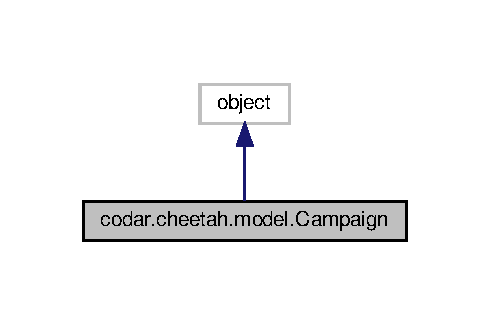
\includegraphics[width=235pt]{classcodar_1_1cheetah_1_1model_1_1_campaign__inherit__graph}
\end{center}
\end{figure}


Collaboration diagram for codar.\+cheetah.\+model.\+Campaign\+:
\nopagebreak
\begin{figure}[H]
\begin{center}
\leavevmode
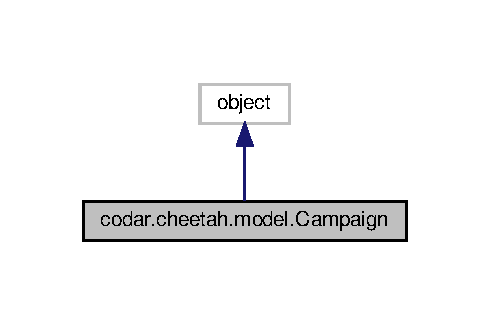
\includegraphics[width=235pt]{classcodar_1_1cheetah_1_1model_1_1_campaign__coll__graph}
\end{center}
\end{figure}
\subsection*{Public Member Functions}
\begin{DoxyCompactItemize}
\item 
\mbox{\Hypertarget{classcodar_1_1cheetah_1_1model_1_1_campaign_ad1b15b5ae37794b2568fe8460f36eab6}\label{classcodar_1_1cheetah_1_1model_1_1_campaign_ad1b15b5ae37794b2568fe8460f36eab6}} 
def {\bfseries \+\_\+\+\_\+init\+\_\+\+\_\+} (self, machine\+\_\+name, app\+\_\+dir)
\item 
def \hyperlink{classcodar_1_1cheetah_1_1model_1_1_campaign_a09266b3421f37a82d8e12c1272e3f54b}{make\+\_\+experiment\+\_\+run\+\_\+dir} (self, output\+\_\+dir, \+\_\+check\+\_\+code\+\_\+paths=True)
\end{DoxyCompactItemize}
\subsection*{Public Attributes}
\begin{DoxyCompactItemize}
\item 
\mbox{\Hypertarget{classcodar_1_1cheetah_1_1model_1_1_campaign_a22d066017db80781e962ce372c32bf79}\label{classcodar_1_1cheetah_1_1model_1_1_campaign_a22d066017db80781e962ce372c32bf79}} 
{\bfseries machine}
\item 
\mbox{\Hypertarget{classcodar_1_1cheetah_1_1model_1_1_campaign_a0d0c15af5ad8c345542eeba939f15ef6}\label{classcodar_1_1cheetah_1_1model_1_1_campaign_a0d0c15af5ad8c345542eeba939f15ef6}} 
{\bfseries app\+\_\+dir}
\item 
\mbox{\Hypertarget{classcodar_1_1cheetah_1_1model_1_1_campaign_ade0d3ba84103ebb3c91252576b3c18f1}\label{classcodar_1_1cheetah_1_1model_1_1_campaign_ade0d3ba84103ebb3c91252576b3c18f1}} 
{\bfseries runs}
\item 
\mbox{\Hypertarget{classcodar_1_1cheetah_1_1model_1_1_campaign_a91554c0c4fc9689aea73d47f9b3c991c}\label{classcodar_1_1cheetah_1_1model_1_1_campaign_a91554c0c4fc9689aea73d47f9b3c991c}} 
{\bfseries inputs}
\item 
\mbox{\Hypertarget{classcodar_1_1cheetah_1_1model_1_1_campaign_ab7a9563b8cc62768d19be6a2f4c7772c}\label{classcodar_1_1cheetah_1_1model_1_1_campaign_ab7a9563b8cc62768d19be6a2f4c7772c}} 
{\bfseries codes}
\item 
\mbox{\Hypertarget{classcodar_1_1cheetah_1_1model_1_1_campaign_a1c6c7a99c27b5ed80721cb4a2328446f}\label{classcodar_1_1cheetah_1_1model_1_1_campaign_a1c6c7a99c27b5ed80721cb4a2328446f}} 
{\bfseries machine\+\_\+scheduler\+\_\+options}
\item 
\mbox{\Hypertarget{classcodar_1_1cheetah_1_1model_1_1_campaign_aa7fbc79a48f35a16bb12db12bef77a20}\label{classcodar_1_1cheetah_1_1model_1_1_campaign_aa7fbc79a48f35a16bb12db12bef77a20}} 
{\bfseries machine\+\_\+app\+\_\+config\+\_\+script}
\end{DoxyCompactItemize}
\subsection*{Static Public Attributes}
\begin{DoxyCompactItemize}
\item 
\mbox{\Hypertarget{classcodar_1_1cheetah_1_1model_1_1_campaign_abc6944cb247705f1e7059d59537836d0}\label{classcodar_1_1cheetah_1_1model_1_1_campaign_abc6944cb247705f1e7059d59537836d0}} 
{\bfseries name} = None
\item 
\mbox{\Hypertarget{classcodar_1_1cheetah_1_1model_1_1_campaign_a963d2407a8818742d80cdabd0b462dc6}\label{classcodar_1_1cheetah_1_1model_1_1_campaign_a963d2407a8818742d80cdabd0b462dc6}} 
list {\bfseries codes} = \mbox{[}$\,$\mbox{]}
\item 
\mbox{\Hypertarget{classcodar_1_1cheetah_1_1model_1_1_campaign_a06c63b2936ba8b23426ce41472dcbfd4}\label{classcodar_1_1cheetah_1_1model_1_1_campaign_a06c63b2936ba8b23426ce41472dcbfd4}} 
list {\bfseries supported\+\_\+machines} = \mbox{[}$\,$\mbox{]}
\item 
\mbox{\Hypertarget{classcodar_1_1cheetah_1_1model_1_1_campaign_a298ec8ce182bf48901b0a40332de3c6d}\label{classcodar_1_1cheetah_1_1model_1_1_campaign_a298ec8ce182bf48901b0a40332de3c6d}} 
list {\bfseries sweeps} = \mbox{[}$\,$\mbox{]}
\item 
\mbox{\Hypertarget{classcodar_1_1cheetah_1_1model_1_1_campaign_a95d21ac374c6126edc3c82b8f953b9af}\label{classcodar_1_1cheetah_1_1model_1_1_campaign_a95d21ac374c6126edc3c82b8f953b9af}} 
list {\bfseries inputs} = \mbox{[}$\,$\mbox{]}
\item 
\mbox{\Hypertarget{classcodar_1_1cheetah_1_1model_1_1_campaign_a7923c1c6debd3f7ce3c1730d21cdfb80}\label{classcodar_1_1cheetah_1_1model_1_1_campaign_a7923c1c6debd3f7ce3c1730d21cdfb80}} 
{\bfseries umask} = None
\item 
\mbox{\Hypertarget{classcodar_1_1cheetah_1_1model_1_1_campaign_a1b3525f75cec5b7d738a1aea32c44612}\label{classcodar_1_1cheetah_1_1model_1_1_campaign_a1b3525f75cec5b7d738a1aea32c44612}} 
bool {\bfseries kill\+\_\+on\+\_\+partial\+\_\+failure} = False
\item 
\mbox{\Hypertarget{classcodar_1_1cheetah_1_1model_1_1_campaign_a86d1217f25978d2210e2ddd6d2a99937}\label{classcodar_1_1cheetah_1_1model_1_1_campaign_a86d1217f25978d2210e2ddd6d2a99937}} 
{\bfseries run\+\_\+post\+\_\+process\+\_\+script} = None
\item 
\mbox{\Hypertarget{classcodar_1_1cheetah_1_1model_1_1_campaign_a063e53373a2750fcdbf7eec7ebaa101b}\label{classcodar_1_1cheetah_1_1model_1_1_campaign_a063e53373a2750fcdbf7eec7ebaa101b}} 
bool {\bfseries run\+\_\+post\+\_\+process\+\_\+stop\+\_\+group\+\_\+on\+\_\+failure} = False
\item 
\mbox{\Hypertarget{classcodar_1_1cheetah_1_1model_1_1_campaign_a434f06408e6b364e0efc232fa107eb33}\label{classcodar_1_1cheetah_1_1model_1_1_campaign_a434f06408e6b364e0efc232fa107eb33}} 
{\bfseries app\+\_\+config\+\_\+scripts} = None
\item 
\mbox{\Hypertarget{classcodar_1_1cheetah_1_1model_1_1_campaign_aa7d421cedfa8ffb615f6fd8f38b208ef}\label{classcodar_1_1cheetah_1_1model_1_1_campaign_aa7d421cedfa8ffb615f6fd8f38b208ef}} 
{\bfseries run\+\_\+dir\+\_\+setup\+\_\+script} = None
\item 
\mbox{\Hypertarget{classcodar_1_1cheetah_1_1model_1_1_campaign_a6c58ab5dac64e6ab4796c6e6de6347c7}\label{classcodar_1_1cheetah_1_1model_1_1_campaign_a6c58ab5dac64e6ab4796c6e6de6347c7}} 
dictionary {\bfseries scheduler\+\_\+options} = \{\}
\item 
\mbox{\Hypertarget{classcodar_1_1cheetah_1_1model_1_1_campaign_a28e44a6ede93e17d40627bd9a31fa8d3}\label{classcodar_1_1cheetah_1_1model_1_1_campaign_a28e44a6ede93e17d40627bd9a31fa8d3}} 
{\bfseries tau\+\_\+config} = None
\item 
\mbox{\Hypertarget{classcodar_1_1cheetah_1_1model_1_1_campaign_af655e512e1d8b7a3bd5104d890dab023}\label{classcodar_1_1cheetah_1_1model_1_1_campaign_af655e512e1d8b7a3bd5104d890dab023}} 
{\bfseries sosd\+\_\+path} = None
\item 
\mbox{\Hypertarget{classcodar_1_1cheetah_1_1model_1_1_campaign_a521eea7dac8df14f3ea9174cd6297340}\label{classcodar_1_1cheetah_1_1model_1_1_campaign_a521eea7dac8df14f3ea9174cd6297340}} 
{\bfseries sos\+\_\+analysis\+\_\+path} = None
\item 
\mbox{\Hypertarget{classcodar_1_1cheetah_1_1model_1_1_campaign_a8cdebf43b605e4ac036fbf4e0b9e7d15}\label{classcodar_1_1cheetah_1_1model_1_1_campaign_a8cdebf43b605e4ac036fbf4e0b9e7d15}} 
int {\bfseries sosd\+\_\+num\+\_\+aggregators} = 1
\item 
\mbox{\Hypertarget{classcodar_1_1cheetah_1_1model_1_1_campaign_a7452ae0f9b6946a5e531cf6bebd55179}\label{classcodar_1_1cheetah_1_1model_1_1_campaign_a7452ae0f9b6946a5e531cf6bebd55179}} 
{\bfseries post\+\_\+process\+\_\+script} = None
\item 
\mbox{\Hypertarget{classcodar_1_1cheetah_1_1model_1_1_campaign_af71218dfabb60e7f23997a0a8f1e1158}\label{classcodar_1_1cheetah_1_1model_1_1_campaign_af71218dfabb60e7f23997a0a8f1e1158}} 
{\bfseries python\+\_\+path} = sys.\+executable
\end{DoxyCompactItemize}


\subsection{Detailed Description}
\begin{DoxyVerb}An experiment class specifies an application, a set of parameter to
sweep over, and a set of supported target machine. A specific instance
binds the experiment to a specific machine within the set of supported
machines, and supports generating a set of scripts to run the experiment
on that machine.\end{DoxyVerb}
 

\subsection{Member Function Documentation}
\mbox{\Hypertarget{classcodar_1_1cheetah_1_1model_1_1_campaign_a09266b3421f37a82d8e12c1272e3f54b}\label{classcodar_1_1cheetah_1_1model_1_1_campaign_a09266b3421f37a82d8e12c1272e3f54b}} 
\index{codar\+::cheetah\+::model\+::\+Campaign@{codar\+::cheetah\+::model\+::\+Campaign}!make\+\_\+experiment\+\_\+run\+\_\+dir@{make\+\_\+experiment\+\_\+run\+\_\+dir}}
\index{make\+\_\+experiment\+\_\+run\+\_\+dir@{make\+\_\+experiment\+\_\+run\+\_\+dir}!codar\+::cheetah\+::model\+::\+Campaign@{codar\+::cheetah\+::model\+::\+Campaign}}
\subsubsection{\texorpdfstring{make\+\_\+experiment\+\_\+run\+\_\+dir()}{make\_experiment\_run\_dir()}}
{\footnotesize\ttfamily def codar.\+cheetah.\+model.\+Campaign.\+make\+\_\+experiment\+\_\+run\+\_\+dir (\begin{DoxyParamCaption}\item[{}]{self,  }\item[{}]{output\+\_\+dir,  }\item[{}]{\+\_\+check\+\_\+code\+\_\+paths = {\ttfamily True} }\end{DoxyParamCaption})}

\begin{DoxyVerb}Produce scripts and directory structure for running the experiment.

Directory structure will be a subdirectory for each scheduler group,
and within each scheduler group directory, a subdirectory for each
run.\end{DoxyVerb}
 

The documentation for this class was generated from the following file\+:\begin{DoxyCompactItemize}
\item 
model.\+py\end{DoxyCompactItemize}

\hypertarget{classcodar_1_1cheetah_1_1exc_1_1_campaign_parse_error}{}\section{codar.\+cheetah.\+exc.\+Campaign\+Parse\+Error Class Reference}
\label{classcodar_1_1cheetah_1_1exc_1_1_campaign_parse_error}\index{codar.\+cheetah.\+exc.\+Campaign\+Parse\+Error@{codar.\+cheetah.\+exc.\+Campaign\+Parse\+Error}}


Inheritance diagram for codar.\+cheetah.\+exc.\+Campaign\+Parse\+Error\+:
\nopagebreak
\begin{figure}[H]
\begin{center}
\leavevmode
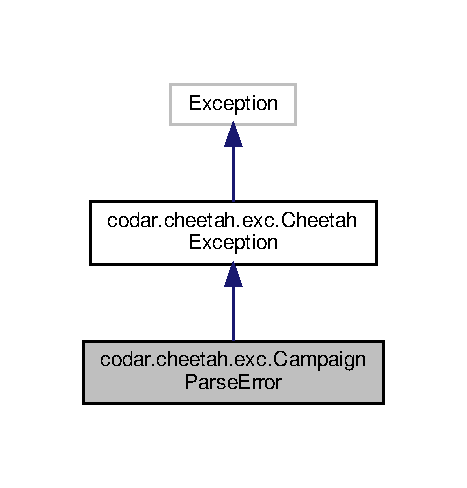
\includegraphics[width=224pt]{classcodar_1_1cheetah_1_1exc_1_1_campaign_parse_error__inherit__graph}
\end{center}
\end{figure}


Collaboration diagram for codar.\+cheetah.\+exc.\+Campaign\+Parse\+Error\+:
\nopagebreak
\begin{figure}[H]
\begin{center}
\leavevmode
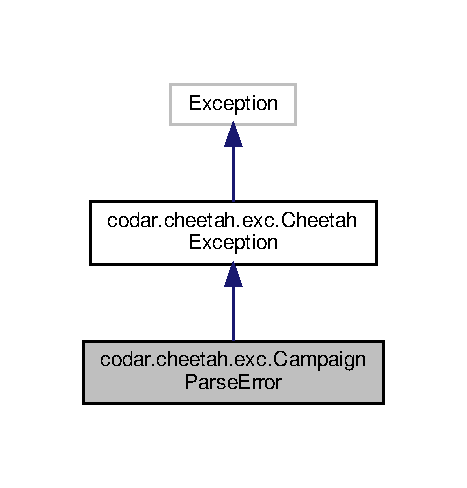
\includegraphics[width=224pt]{classcodar_1_1cheetah_1_1exc_1_1_campaign_parse_error__coll__graph}
\end{center}
\end{figure}


\subsection{Detailed Description}


Definition at line 16 of file exc.\+py.



The documentation for this class was generated from the following file\+:\begin{DoxyCompactItemize}
\item 
cheetah/\hyperlink{cheetah_2exc_8py}{exc.\+py}\end{DoxyCompactItemize}

\hypertarget{classcodar_1_1cheetah_1_1exc_1_1_cheetah_exception}{}\section{codar.\+cheetah.\+exc.\+Cheetah\+Exception Class Reference}
\label{classcodar_1_1cheetah_1_1exc_1_1_cheetah_exception}\index{codar.\+cheetah.\+exc.\+Cheetah\+Exception@{codar.\+cheetah.\+exc.\+Cheetah\+Exception}}


Inheritance diagram for codar.\+cheetah.\+exc.\+Cheetah\+Exception\+:
\nopagebreak
\begin{figure}[H]
\begin{center}
\leavevmode
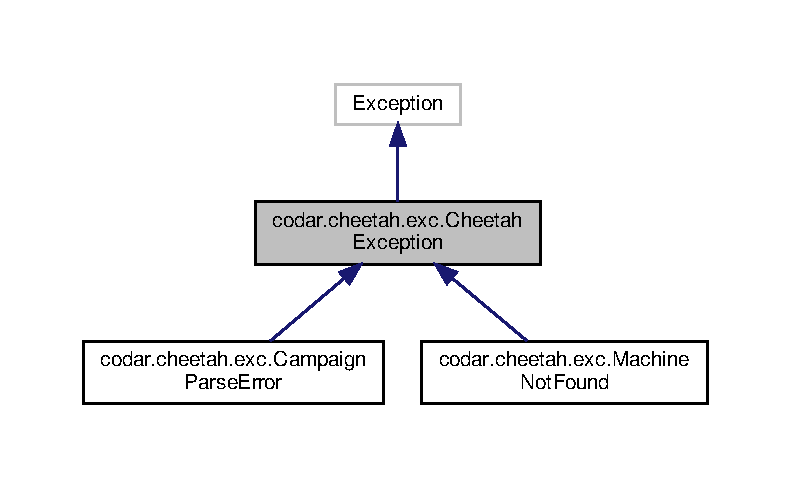
\includegraphics[width=350pt]{classcodar_1_1cheetah_1_1exc_1_1_cheetah_exception__inherit__graph}
\end{center}
\end{figure}


Collaboration diagram for codar.\+cheetah.\+exc.\+Cheetah\+Exception\+:
\nopagebreak
\begin{figure}[H]
\begin{center}
\leavevmode
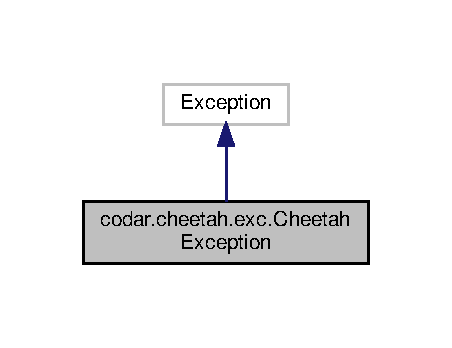
\includegraphics[width=217pt]{classcodar_1_1cheetah_1_1exc_1_1_cheetah_exception__coll__graph}
\end{center}
\end{figure}


The documentation for this class was generated from the following file\+:\begin{DoxyCompactItemize}
\item 
exc.\+py\end{DoxyCompactItemize}

\hypertarget{classcodar_1_1cheetah_1_1parameters_1_1_code_command}{}\section{codar.\+cheetah.\+parameters.\+Code\+Command Class Reference}
\label{classcodar_1_1cheetah_1_1parameters_1_1_code_command}\index{codar.\+cheetah.\+parameters.\+Code\+Command@{codar.\+cheetah.\+parameters.\+Code\+Command}}


Inheritance diagram for codar.\+cheetah.\+parameters.\+Code\+Command\+:
\nopagebreak
\begin{figure}[H]
\begin{center}
\leavevmode
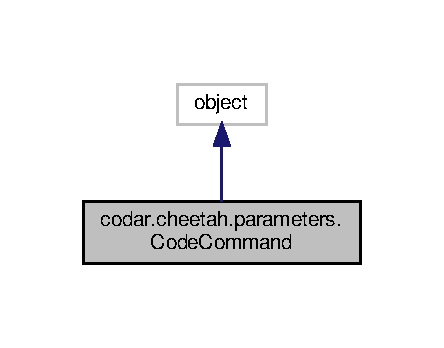
\includegraphics[width=213pt]{classcodar_1_1cheetah_1_1parameters_1_1_code_command__inherit__graph}
\end{center}
\end{figure}


Collaboration diagram for codar.\+cheetah.\+parameters.\+Code\+Command\+:
\nopagebreak
\begin{figure}[H]
\begin{center}
\leavevmode
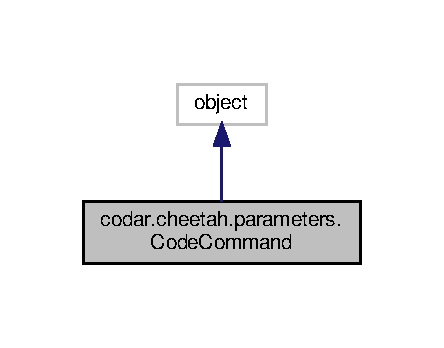
\includegraphics[width=213pt]{classcodar_1_1cheetah_1_1parameters_1_1_code_command__coll__graph}
\end{center}
\end{figure}
\subsection*{Public Member Functions}
\begin{DoxyCompactItemize}
\item 
\mbox{\Hypertarget{classcodar_1_1cheetah_1_1parameters_1_1_code_command_a706c2fb3961bd3a8eb91d1034020893c}\label{classcodar_1_1cheetah_1_1parameters_1_1_code_command_a706c2fb3961bd3a8eb91d1034020893c}} 
def {\bfseries \+\_\+\+\_\+init\+\_\+\+\_\+} (self, target)
\item 
def \hyperlink{classcodar_1_1cheetah_1_1parameters_1_1_code_command_a869d18602cb7e516157c871a6a80527e}{add\+\_\+arg} (self, position, value)
\item 
\mbox{\Hypertarget{classcodar_1_1cheetah_1_1parameters_1_1_code_command_ab2d06207053333ebd442800d991a5056}\label{classcodar_1_1cheetah_1_1parameters_1_1_code_command_ab2d06207053333ebd442800d991a5056}} 
def {\bfseries add\+\_\+option} (self, option, value)
\item 
\mbox{\Hypertarget{classcodar_1_1cheetah_1_1parameters_1_1_code_command_a94799c614d5777f929817d9a855a0f88}\label{classcodar_1_1cheetah_1_1parameters_1_1_code_command_a94799c614d5777f929817d9a855a0f88}} 
def {\bfseries get\+\_\+argv} (self)
\end{DoxyCompactItemize}
\subsection*{Public Attributes}
\begin{DoxyCompactItemize}
\item 
\mbox{\Hypertarget{classcodar_1_1cheetah_1_1parameters_1_1_code_command_a52652e8b3bc2c4bcf55f7edd13f8258c}\label{classcodar_1_1cheetah_1_1parameters_1_1_code_command_a52652e8b3bc2c4bcf55f7edd13f8258c}} 
{\bfseries target}
\item 
\mbox{\Hypertarget{classcodar_1_1cheetah_1_1parameters_1_1_code_command_a5130989e66f83d0d6750f32a84edf44e}\label{classcodar_1_1cheetah_1_1parameters_1_1_code_command_a5130989e66f83d0d6750f32a84edf44e}} 
{\bfseries args}
\item 
\mbox{\Hypertarget{classcodar_1_1cheetah_1_1parameters_1_1_code_command_a7b7c38e78d429b1395daf3e6b199aafe}\label{classcodar_1_1cheetah_1_1parameters_1_1_code_command_a7b7c38e78d429b1395daf3e6b199aafe}} 
{\bfseries options}
\end{DoxyCompactItemize}


\subsection{Detailed Description}
\begin{DoxyVerb}Helper class to build up command args and options as we go. Does not
know about the path to it's executable, that is part of the execution
environment which is added during realization.
\end{DoxyVerb}
 

\subsection{Member Function Documentation}
\mbox{\Hypertarget{classcodar_1_1cheetah_1_1parameters_1_1_code_command_a869d18602cb7e516157c871a6a80527e}\label{classcodar_1_1cheetah_1_1parameters_1_1_code_command_a869d18602cb7e516157c871a6a80527e}} 
\index{codar\+::cheetah\+::parameters\+::\+Code\+Command@{codar\+::cheetah\+::parameters\+::\+Code\+Command}!add\+\_\+arg@{add\+\_\+arg}}
\index{add\+\_\+arg@{add\+\_\+arg}!codar\+::cheetah\+::parameters\+::\+Code\+Command@{codar\+::cheetah\+::parameters\+::\+Code\+Command}}
\subsubsection{\texorpdfstring{add\+\_\+arg()}{add\_arg()}}
{\footnotesize\ttfamily def codar.\+cheetah.\+parameters.\+Code\+Command.\+add\+\_\+arg (\begin{DoxyParamCaption}\item[{}]{self,  }\item[{}]{position,  }\item[{}]{value }\end{DoxyParamCaption})}

\begin{DoxyVerb}Allows adding positional args out of order.

TODO: better error handling.
\end{DoxyVerb}
 

The documentation for this class was generated from the following file\+:\begin{DoxyCompactItemize}
\item 
parameters.\+py\end{DoxyCompactItemize}

\hypertarget{classcodar_1_1cheetah_1_1parameters_1_1_instance}{}\section{codar.\+cheetah.\+parameters.\+Instance Class Reference}
\label{classcodar_1_1cheetah_1_1parameters_1_1_instance}\index{codar.\+cheetah.\+parameters.\+Instance@{codar.\+cheetah.\+parameters.\+Instance}}


Inheritance diagram for codar.\+cheetah.\+parameters.\+Instance\+:
\nopagebreak
\begin{figure}[H]
\begin{center}
\leavevmode
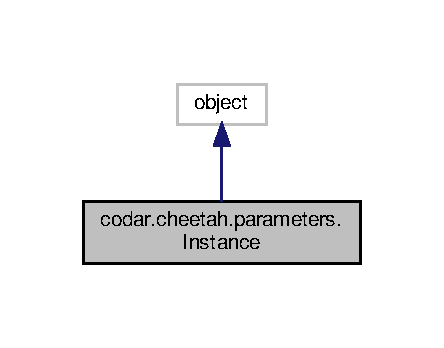
\includegraphics[width=213pt]{classcodar_1_1cheetah_1_1parameters_1_1_instance__inherit__graph}
\end{center}
\end{figure}


Collaboration diagram for codar.\+cheetah.\+parameters.\+Instance\+:
\nopagebreak
\begin{figure}[H]
\begin{center}
\leavevmode
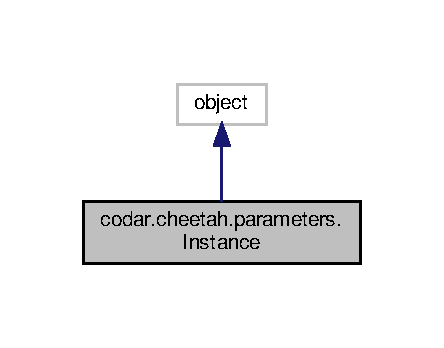
\includegraphics[width=213pt]{classcodar_1_1cheetah_1_1parameters_1_1_instance__coll__graph}
\end{center}
\end{figure}
\subsection*{Public Member Functions}
\begin{DoxyCompactItemize}
\item 
\mbox{\Hypertarget{classcodar_1_1cheetah_1_1parameters_1_1_instance_abc52192d373d1741efd7566d320d68c1}\label{classcodar_1_1cheetah_1_1parameters_1_1_instance_abc52192d373d1741efd7566d320d68c1}} 
def {\bfseries \+\_\+\+\_\+init\+\_\+\+\_\+} (self)
\item 
\mbox{\Hypertarget{classcodar_1_1cheetah_1_1parameters_1_1_instance_a600511535b03f1796f9a0d84b654e113}\label{classcodar_1_1cheetah_1_1parameters_1_1_instance_a600511535b03f1796f9a0d84b654e113}} 
def {\bfseries add\+\_\+parameter} (self, p, idx)
\item 
def \hyperlink{classcodar_1_1cheetah_1_1parameters_1_1_instance_a4a943c0f5f3afe8b9a4ff9b238aab766}{parameter\+\_\+values} (self)
\item 
def \hyperlink{classcodar_1_1cheetah_1_1parameters_1_1_instance_a417d9d44a5eb0e0b8812fc427ddc4435}{code\+\_\+commands} (self)
\item 
def \hyperlink{classcodar_1_1cheetah_1_1parameters_1_1_instance_a4ee126bbceeb792914185ca9fbe59101}{get\+\_\+codes\+\_\+argv} (self)
\item 
def \hyperlink{classcodar_1_1cheetah_1_1parameters_1_1_instance_a053717fc3ee7840a7c32173f15e99ae3}{as\+\_\+string} (self)
\item 
def \hyperlink{classcodar_1_1cheetah_1_1parameters_1_1_instance_ab1187231851e554aa1e95f7e7eee7b77}{get\+\_\+parameter\+\_\+values\+\_\+by\+\_\+type} (self, param\+\_\+class)
\item 
\mbox{\Hypertarget{classcodar_1_1cheetah_1_1parameters_1_1_instance_add69b3c4bcc37530ba16bd77cd843872}\label{classcodar_1_1cheetah_1_1parameters_1_1_instance_add69b3c4bcc37530ba16bd77cd843872}} 
def {\bfseries get\+\_\+nprocs} (self, target)
\item 
def \hyperlink{classcodar_1_1cheetah_1_1parameters_1_1_instance_ae978374d4b5e01c2764b9513ae38a961}{as\+\_\+dict} (self)
\end{DoxyCompactItemize}


\subsection{Detailed Description}
\begin{DoxyVerb}Represent an instance of an application with fixed parameters. An
application may consistent of multiple codes running at the same time,
and multiple middlewear layers (scheduler like PBS, runner like aprun,
or swift), all of which may have their own parameters.

Abstractly, an instance is a two-level nested dict, where the first
level indicates the target for a parameter (application code or
middlewear), and the second level contains the parameter values for that
target.
\end{DoxyVerb}
 

\subsection{Member Function Documentation}
\mbox{\Hypertarget{classcodar_1_1cheetah_1_1parameters_1_1_instance_ae978374d4b5e01c2764b9513ae38a961}\label{classcodar_1_1cheetah_1_1parameters_1_1_instance_ae978374d4b5e01c2764b9513ae38a961}} 
\index{codar\+::cheetah\+::parameters\+::\+Instance@{codar\+::cheetah\+::parameters\+::\+Instance}!as\+\_\+dict@{as\+\_\+dict}}
\index{as\+\_\+dict@{as\+\_\+dict}!codar\+::cheetah\+::parameters\+::\+Instance@{codar\+::cheetah\+::parameters\+::\+Instance}}
\subsubsection{\texorpdfstring{as\+\_\+dict()}{as\_dict()}}
{\footnotesize\ttfamily def codar.\+cheetah.\+parameters.\+Instance.\+as\+\_\+dict (\begin{DoxyParamCaption}\item[{}]{self }\end{DoxyParamCaption})}

\begin{DoxyVerb}Produce dict (mainly for for JSON seriliazation) with keys based on
parameter names. This ignores the type of the param, it's just the
name value pairs.
\end{DoxyVerb}
 \mbox{\Hypertarget{classcodar_1_1cheetah_1_1parameters_1_1_instance_a053717fc3ee7840a7c32173f15e99ae3}\label{classcodar_1_1cheetah_1_1parameters_1_1_instance_a053717fc3ee7840a7c32173f15e99ae3}} 
\index{codar\+::cheetah\+::parameters\+::\+Instance@{codar\+::cheetah\+::parameters\+::\+Instance}!as\+\_\+string@{as\+\_\+string}}
\index{as\+\_\+string@{as\+\_\+string}!codar\+::cheetah\+::parameters\+::\+Instance@{codar\+::cheetah\+::parameters\+::\+Instance}}
\subsubsection{\texorpdfstring{as\+\_\+string()}{as\_string()}}
{\footnotesize\ttfamily def codar.\+cheetah.\+parameters.\+Instance.\+as\+\_\+string (\begin{DoxyParamCaption}\item[{}]{self }\end{DoxyParamCaption})}

\begin{DoxyVerb}Get a command line like value for the instance. Note that this
only includes positional and option command line args, not config
args like adios XML. TODO: deprecate??\end{DoxyVerb}
 \mbox{\Hypertarget{classcodar_1_1cheetah_1_1parameters_1_1_instance_a417d9d44a5eb0e0b8812fc427ddc4435}\label{classcodar_1_1cheetah_1_1parameters_1_1_instance_a417d9d44a5eb0e0b8812fc427ddc4435}} 
\index{codar\+::cheetah\+::parameters\+::\+Instance@{codar\+::cheetah\+::parameters\+::\+Instance}!code\+\_\+commands@{code\+\_\+commands}}
\index{code\+\_\+commands@{code\+\_\+commands}!codar\+::cheetah\+::parameters\+::\+Instance@{codar\+::cheetah\+::parameters\+::\+Instance}}
\subsubsection{\texorpdfstring{code\+\_\+commands()}{code\_commands()}}
{\footnotesize\ttfamily def codar.\+cheetah.\+parameters.\+Instance.\+code\+\_\+commands (\begin{DoxyParamCaption}\item[{}]{self }\end{DoxyParamCaption})}

\begin{DoxyVerb}Wrapper to allow delayed calculation of derived parameter values.\end{DoxyVerb}
 \mbox{\Hypertarget{classcodar_1_1cheetah_1_1parameters_1_1_instance_a4ee126bbceeb792914185ca9fbe59101}\label{classcodar_1_1cheetah_1_1parameters_1_1_instance_a4ee126bbceeb792914185ca9fbe59101}} 
\index{codar\+::cheetah\+::parameters\+::\+Instance@{codar\+::cheetah\+::parameters\+::\+Instance}!get\+\_\+codes\+\_\+argv@{get\+\_\+codes\+\_\+argv}}
\index{get\+\_\+codes\+\_\+argv@{get\+\_\+codes\+\_\+argv}!codar\+::cheetah\+::parameters\+::\+Instance@{codar\+::cheetah\+::parameters\+::\+Instance}}
\subsubsection{\texorpdfstring{get\+\_\+codes\+\_\+argv()}{get\_codes\_argv()}}
{\footnotesize\ttfamily def codar.\+cheetah.\+parameters.\+Instance.\+get\+\_\+codes\+\_\+argv (\begin{DoxyParamCaption}\item[{}]{self }\end{DoxyParamCaption})}

\begin{DoxyVerb}Get an _unordered_ dict mapping code name to list of args for
that code. Higher levels of model are responsible for re-ordering
as needed.\end{DoxyVerb}
 \mbox{\Hypertarget{classcodar_1_1cheetah_1_1parameters_1_1_instance_ab1187231851e554aa1e95f7e7eee7b77}\label{classcodar_1_1cheetah_1_1parameters_1_1_instance_ab1187231851e554aa1e95f7e7eee7b77}} 
\index{codar\+::cheetah\+::parameters\+::\+Instance@{codar\+::cheetah\+::parameters\+::\+Instance}!get\+\_\+parameter\+\_\+values\+\_\+by\+\_\+type@{get\+\_\+parameter\+\_\+values\+\_\+by\+\_\+type}}
\index{get\+\_\+parameter\+\_\+values\+\_\+by\+\_\+type@{get\+\_\+parameter\+\_\+values\+\_\+by\+\_\+type}!codar\+::cheetah\+::parameters\+::\+Instance@{codar\+::cheetah\+::parameters\+::\+Instance}}
\subsubsection{\texorpdfstring{get\+\_\+parameter\+\_\+values\+\_\+by\+\_\+type()}{get\_parameter\_values\_by\_type()}}
{\footnotesize\ttfamily def codar.\+cheetah.\+parameters.\+Instance.\+get\+\_\+parameter\+\_\+values\+\_\+by\+\_\+type (\begin{DoxyParamCaption}\item[{}]{self,  }\item[{}]{param\+\_\+class }\end{DoxyParamCaption})}

\begin{DoxyVerb}Get a list of ParamaterValues of the specified type in the instance.
\end{DoxyVerb}
 \mbox{\Hypertarget{classcodar_1_1cheetah_1_1parameters_1_1_instance_a4a943c0f5f3afe8b9a4ff9b238aab766}\label{classcodar_1_1cheetah_1_1parameters_1_1_instance_a4a943c0f5f3afe8b9a4ff9b238aab766}} 
\index{codar\+::cheetah\+::parameters\+::\+Instance@{codar\+::cheetah\+::parameters\+::\+Instance}!parameter\+\_\+values@{parameter\+\_\+values}}
\index{parameter\+\_\+values@{parameter\+\_\+values}!codar\+::cheetah\+::parameters\+::\+Instance@{codar\+::cheetah\+::parameters\+::\+Instance}}
\subsubsection{\texorpdfstring{parameter\+\_\+values()}{parameter\_values()}}
{\footnotesize\ttfamily def codar.\+cheetah.\+parameters.\+Instance.\+parameter\+\_\+values (\begin{DoxyParamCaption}\item[{}]{self }\end{DoxyParamCaption})}

\begin{DoxyVerb}Wrapper to allow delayed calculation of derived parameter values.\end{DoxyVerb}
 

The documentation for this class was generated from the following file\+:\begin{DoxyCompactItemize}
\item 
parameters.\+py\end{DoxyCompactItemize}

\hypertarget{classcodar_1_1savanna_1_1scheduler_1_1_job_list}{}\section{codar.\+savanna.\+scheduler.\+Job\+List Class Reference}
\label{classcodar_1_1savanna_1_1scheduler_1_1_job_list}\index{codar.\+savanna.\+scheduler.\+Job\+List@{codar.\+savanna.\+scheduler.\+Job\+List}}


Inheritance diagram for codar.\+savanna.\+scheduler.\+Job\+List\+:
\nopagebreak
\begin{figure}[H]
\begin{center}
\leavevmode
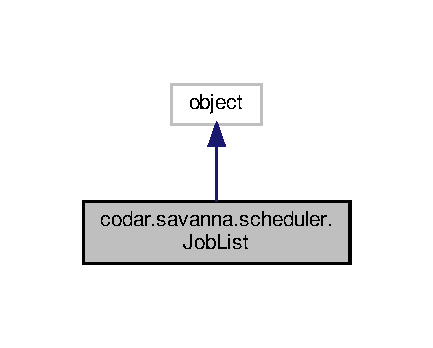
\includegraphics[width=208pt]{classcodar_1_1savanna_1_1scheduler_1_1_job_list__inherit__graph}
\end{center}
\end{figure}


Collaboration diagram for codar.\+savanna.\+scheduler.\+Job\+List\+:
\nopagebreak
\begin{figure}[H]
\begin{center}
\leavevmode
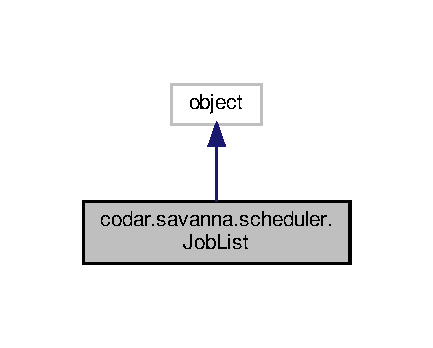
\includegraphics[width=208pt]{classcodar_1_1savanna_1_1scheduler_1_1_job_list__coll__graph}
\end{center}
\end{figure}
\subsection*{Public Member Functions}
\begin{DoxyCompactItemize}
\item 
def \hyperlink{classcodar_1_1savanna_1_1scheduler_1_1_job_list_a692f67c81a57a97d01e899aa1f468435}{\+\_\+\+\_\+init\+\_\+\+\_\+} (self, costfn, initial\+\_\+jobs=None)
\item 
def \hyperlink{classcodar_1_1savanna_1_1scheduler_1_1_job_list_a235fcb4111e178e10fc7ab644bf9b531}{add\+\_\+job} (self, job)
\item 
def \hyperlink{classcodar_1_1savanna_1_1scheduler_1_1_job_list_a5aacbb616928bc7e9078ea08afe8d5ef}{pop\+\_\+job} (self, max\+\_\+cost)
\item 
def \hyperlink{classcodar_1_1savanna_1_1scheduler_1_1_job_list_a2ff2f963962e0c5cf5dac35c3cd37647}{\+\_\+\+\_\+len\+\_\+\+\_\+} (self)
\end{DoxyCompactItemize}


\subsection{Detailed Description}
\begin{DoxyVerb}Manage a job list that can find and remove the highest cost job that
doesn't exceed max_cost and insert new jobs.

The job objects can be any type, but a key function must be provided
that takes an instance of a job and returns it's cost.

Uses a coordinated pair of sort list for costs and jobs, along with
the bisect module. A linked list might be more efficient, since the
list copy on insert and delete may dominate the time to do a linear
search of a small list, but it's likely fine either way for the
sizes we will encounter.\end{DoxyVerb}
 

Definition at line 18 of file scheduler.\+py.



\subsection{Constructor \& Destructor Documentation}
\mbox{\Hypertarget{classcodar_1_1savanna_1_1scheduler_1_1_job_list_a692f67c81a57a97d01e899aa1f468435}\label{classcodar_1_1savanna_1_1scheduler_1_1_job_list_a692f67c81a57a97d01e899aa1f468435}} 
\index{codar\+::savanna\+::scheduler\+::\+Job\+List@{codar\+::savanna\+::scheduler\+::\+Job\+List}!\+\_\+\+\_\+init\+\_\+\+\_\+@{\+\_\+\+\_\+init\+\_\+\+\_\+}}
\index{\+\_\+\+\_\+init\+\_\+\+\_\+@{\+\_\+\+\_\+init\+\_\+\+\_\+}!codar\+::savanna\+::scheduler\+::\+Job\+List@{codar\+::savanna\+::scheduler\+::\+Job\+List}}
\subsubsection{\texorpdfstring{\+\_\+\+\_\+init\+\_\+\+\_\+()}{\_\_init\_\_()}}
{\footnotesize\ttfamily def codar.\+savanna.\+scheduler.\+Job\+List.\+\_\+\+\_\+init\+\_\+\+\_\+ (\begin{DoxyParamCaption}\item[{}]{self,  }\item[{}]{costfn,  }\item[{}]{initial\+\_\+jobs = {\ttfamily None} }\end{DoxyParamCaption})}



Definition at line 30 of file scheduler.\+py.



\subsection{Member Function Documentation}
\mbox{\Hypertarget{classcodar_1_1savanna_1_1scheduler_1_1_job_list_a2ff2f963962e0c5cf5dac35c3cd37647}\label{classcodar_1_1savanna_1_1scheduler_1_1_job_list_a2ff2f963962e0c5cf5dac35c3cd37647}} 
\index{codar\+::savanna\+::scheduler\+::\+Job\+List@{codar\+::savanna\+::scheduler\+::\+Job\+List}!\+\_\+\+\_\+len\+\_\+\+\_\+@{\+\_\+\+\_\+len\+\_\+\+\_\+}}
\index{\+\_\+\+\_\+len\+\_\+\+\_\+@{\+\_\+\+\_\+len\+\_\+\+\_\+}!codar\+::savanna\+::scheduler\+::\+Job\+List@{codar\+::savanna\+::scheduler\+::\+Job\+List}}
\subsubsection{\texorpdfstring{\+\_\+\+\_\+len\+\_\+\+\_\+()}{\_\_len\_\_()}}
{\footnotesize\ttfamily def codar.\+savanna.\+scheduler.\+Job\+List.\+\_\+\+\_\+len\+\_\+\+\_\+ (\begin{DoxyParamCaption}\item[{}]{self }\end{DoxyParamCaption})}



Definition at line 63 of file scheduler.\+py.

\mbox{\Hypertarget{classcodar_1_1savanna_1_1scheduler_1_1_job_list_a235fcb4111e178e10fc7ab644bf9b531}\label{classcodar_1_1savanna_1_1scheduler_1_1_job_list_a235fcb4111e178e10fc7ab644bf9b531}} 
\index{codar\+::savanna\+::scheduler\+::\+Job\+List@{codar\+::savanna\+::scheduler\+::\+Job\+List}!add\+\_\+job@{add\+\_\+job}}
\index{add\+\_\+job@{add\+\_\+job}!codar\+::savanna\+::scheduler\+::\+Job\+List@{codar\+::savanna\+::scheduler\+::\+Job\+List}}
\subsubsection{\texorpdfstring{add\+\_\+job()}{add\_job()}}
{\footnotesize\ttfamily def codar.\+savanna.\+scheduler.\+Job\+List.\+add\+\_\+job (\begin{DoxyParamCaption}\item[{}]{self,  }\item[{}]{job }\end{DoxyParamCaption})}



Definition at line 41 of file scheduler.\+py.

\mbox{\Hypertarget{classcodar_1_1savanna_1_1scheduler_1_1_job_list_a5aacbb616928bc7e9078ea08afe8d5ef}\label{classcodar_1_1savanna_1_1scheduler_1_1_job_list_a5aacbb616928bc7e9078ea08afe8d5ef}} 
\index{codar\+::savanna\+::scheduler\+::\+Job\+List@{codar\+::savanna\+::scheduler\+::\+Job\+List}!pop\+\_\+job@{pop\+\_\+job}}
\index{pop\+\_\+job@{pop\+\_\+job}!codar\+::savanna\+::scheduler\+::\+Job\+List@{codar\+::savanna\+::scheduler\+::\+Job\+List}}
\subsubsection{\texorpdfstring{pop\+\_\+job()}{pop\_job()}}
{\footnotesize\ttfamily def codar.\+savanna.\+scheduler.\+Job\+List.\+pop\+\_\+job (\begin{DoxyParamCaption}\item[{}]{self,  }\item[{}]{max\+\_\+cost }\end{DoxyParamCaption})}

\begin{DoxyVerb}Get the highest cost job that doesn't exceed max_cost, and remove
it from the job list. Raises IndexError if the job list is empty,
returns None if no suitable jobs exist in the list.\end{DoxyVerb}
 

Definition at line 48 of file scheduler.\+py.



The documentation for this class was generated from the following file\+:\begin{DoxyCompactItemize}
\item 
\hyperlink{scheduler_8py}{scheduler.\+py}\end{DoxyCompactItemize}

\hypertarget{classcodar_1_1savanna_1_1producer_1_1_j_s_o_n_file_pipeline_reader}{}\section{codar.\+savanna.\+producer.\+J\+S\+O\+N\+File\+Pipeline\+Reader Class Reference}
\label{classcodar_1_1savanna_1_1producer_1_1_j_s_o_n_file_pipeline_reader}\index{codar.\+savanna.\+producer.\+J\+S\+O\+N\+File\+Pipeline\+Reader@{codar.\+savanna.\+producer.\+J\+S\+O\+N\+File\+Pipeline\+Reader}}


Inheritance diagram for codar.\+savanna.\+producer.\+J\+S\+O\+N\+File\+Pipeline\+Reader\+:
\nopagebreak
\begin{figure}[H]
\begin{center}
\leavevmode
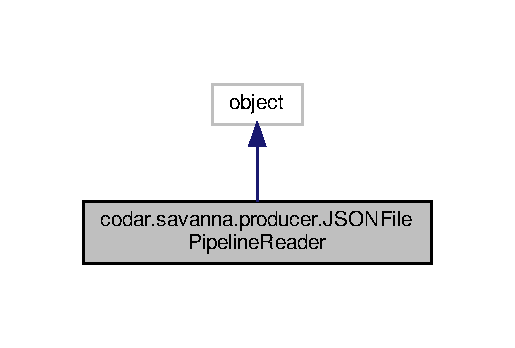
\includegraphics[width=247pt]{classcodar_1_1savanna_1_1producer_1_1_j_s_o_n_file_pipeline_reader__inherit__graph}
\end{center}
\end{figure}


Collaboration diagram for codar.\+savanna.\+producer.\+J\+S\+O\+N\+File\+Pipeline\+Reader\+:
\nopagebreak
\begin{figure}[H]
\begin{center}
\leavevmode
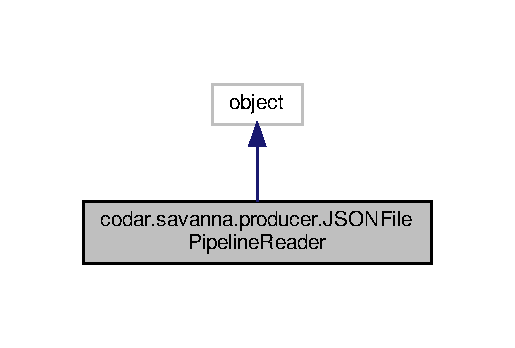
\includegraphics[width=247pt]{classcodar_1_1savanna_1_1producer_1_1_j_s_o_n_file_pipeline_reader__coll__graph}
\end{center}
\end{figure}
\subsection*{Public Member Functions}
\begin{DoxyCompactItemize}
\item 
def \hyperlink{classcodar_1_1savanna_1_1producer_1_1_j_s_o_n_file_pipeline_reader_a55313d819000a60b4c1d0acc6723722b}{\+\_\+\+\_\+init\+\_\+\+\_\+} (self, \hyperlink{classcodar_1_1savanna_1_1producer_1_1_j_s_o_n_file_pipeline_reader_a492f862e3d8692400cc29b11df5cf137}{file\+\_\+path})
\item 
def \hyperlink{classcodar_1_1savanna_1_1producer_1_1_j_s_o_n_file_pipeline_reader_a1b4cf622fdd2146181d5776f044c97c6}{read\+\_\+pipelines} (self)
\end{DoxyCompactItemize}
\subsection*{Public Attributes}
\begin{DoxyCompactItemize}
\item 
\hyperlink{classcodar_1_1savanna_1_1producer_1_1_j_s_o_n_file_pipeline_reader_a492f862e3d8692400cc29b11df5cf137}{file\+\_\+path}
\end{DoxyCompactItemize}


\subsection{Detailed Description}
\begin{DoxyVerb}Load pipelines from a file formatted as a new line separated list of
JSON documents. Each JSON document must be a list containing dictionaries,
each dictionary discribing a code to run as part of the pipeline.\end{DoxyVerb}
 

Definition at line 12 of file producer.\+py.



\subsection{Constructor \& Destructor Documentation}
\mbox{\Hypertarget{classcodar_1_1savanna_1_1producer_1_1_j_s_o_n_file_pipeline_reader_a55313d819000a60b4c1d0acc6723722b}\label{classcodar_1_1savanna_1_1producer_1_1_j_s_o_n_file_pipeline_reader_a55313d819000a60b4c1d0acc6723722b}} 
\index{codar\+::savanna\+::producer\+::\+J\+S\+O\+N\+File\+Pipeline\+Reader@{codar\+::savanna\+::producer\+::\+J\+S\+O\+N\+File\+Pipeline\+Reader}!\+\_\+\+\_\+init\+\_\+\+\_\+@{\+\_\+\+\_\+init\+\_\+\+\_\+}}
\index{\+\_\+\+\_\+init\+\_\+\+\_\+@{\+\_\+\+\_\+init\+\_\+\+\_\+}!codar\+::savanna\+::producer\+::\+J\+S\+O\+N\+File\+Pipeline\+Reader@{codar\+::savanna\+::producer\+::\+J\+S\+O\+N\+File\+Pipeline\+Reader}}
\subsubsection{\texorpdfstring{\+\_\+\+\_\+init\+\_\+\+\_\+()}{\_\_init\_\_()}}
{\footnotesize\ttfamily def codar.\+savanna.\+producer.\+J\+S\+O\+N\+File\+Pipeline\+Reader.\+\_\+\+\_\+init\+\_\+\+\_\+ (\begin{DoxyParamCaption}\item[{}]{self,  }\item[{}]{file\+\_\+path }\end{DoxyParamCaption})}



Definition at line 17 of file producer.\+py.



\subsection{Member Function Documentation}
\mbox{\Hypertarget{classcodar_1_1savanna_1_1producer_1_1_j_s_o_n_file_pipeline_reader_a1b4cf622fdd2146181d5776f044c97c6}\label{classcodar_1_1savanna_1_1producer_1_1_j_s_o_n_file_pipeline_reader_a1b4cf622fdd2146181d5776f044c97c6}} 
\index{codar\+::savanna\+::producer\+::\+J\+S\+O\+N\+File\+Pipeline\+Reader@{codar\+::savanna\+::producer\+::\+J\+S\+O\+N\+File\+Pipeline\+Reader}!read\+\_\+pipelines@{read\+\_\+pipelines}}
\index{read\+\_\+pipelines@{read\+\_\+pipelines}!codar\+::savanna\+::producer\+::\+J\+S\+O\+N\+File\+Pipeline\+Reader@{codar\+::savanna\+::producer\+::\+J\+S\+O\+N\+File\+Pipeline\+Reader}}
\subsubsection{\texorpdfstring{read\+\_\+pipelines()}{read\_pipelines()}}
{\footnotesize\ttfamily def codar.\+savanna.\+producer.\+J\+S\+O\+N\+File\+Pipeline\+Reader.\+read\+\_\+pipelines (\begin{DoxyParamCaption}\item[{}]{self }\end{DoxyParamCaption})}



Definition at line 20 of file producer.\+py.



\subsection{Member Data Documentation}
\mbox{\Hypertarget{classcodar_1_1savanna_1_1producer_1_1_j_s_o_n_file_pipeline_reader_a492f862e3d8692400cc29b11df5cf137}\label{classcodar_1_1savanna_1_1producer_1_1_j_s_o_n_file_pipeline_reader_a492f862e3d8692400cc29b11df5cf137}} 
\index{codar\+::savanna\+::producer\+::\+J\+S\+O\+N\+File\+Pipeline\+Reader@{codar\+::savanna\+::producer\+::\+J\+S\+O\+N\+File\+Pipeline\+Reader}!file\+\_\+path@{file\+\_\+path}}
\index{file\+\_\+path@{file\+\_\+path}!codar\+::savanna\+::producer\+::\+J\+S\+O\+N\+File\+Pipeline\+Reader@{codar\+::savanna\+::producer\+::\+J\+S\+O\+N\+File\+Pipeline\+Reader}}
\subsubsection{\texorpdfstring{file\+\_\+path}{file\_path}}
{\footnotesize\ttfamily codar.\+savanna.\+producer.\+J\+S\+O\+N\+File\+Pipeline\+Reader.\+file\+\_\+path}



Definition at line 18 of file producer.\+py.



The documentation for this class was generated from the following file\+:\begin{DoxyCompactItemize}
\item 
\hyperlink{producer_8py}{producer.\+py}\end{DoxyCompactItemize}

\hypertarget{classcodar_1_1cheetah_1_1launchers_1_1_launcher}{}\section{codar.\+cheetah.\+launchers.\+Launcher Class Reference}
\label{classcodar_1_1cheetah_1_1launchers_1_1_launcher}\index{codar.\+cheetah.\+launchers.\+Launcher@{codar.\+cheetah.\+launchers.\+Launcher}}


Inheritance diagram for codar.\+cheetah.\+launchers.\+Launcher\+:
\nopagebreak
\begin{figure}[H]
\begin{center}
\leavevmode
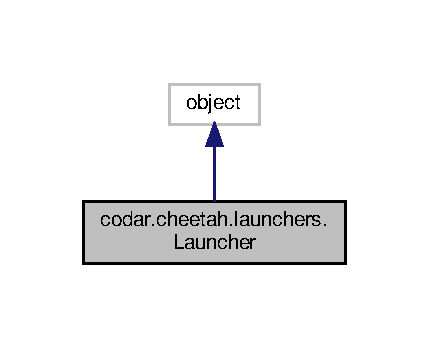
\includegraphics[width=206pt]{classcodar_1_1cheetah_1_1launchers_1_1_launcher__inherit__graph}
\end{center}
\end{figure}


Collaboration diagram for codar.\+cheetah.\+launchers.\+Launcher\+:
\nopagebreak
\begin{figure}[H]
\begin{center}
\leavevmode
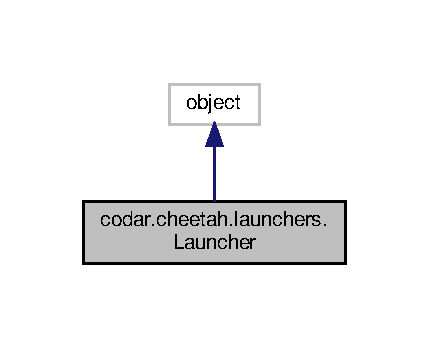
\includegraphics[width=206pt]{classcodar_1_1cheetah_1_1launchers_1_1_launcher__coll__graph}
\end{center}
\end{figure}
\subsection*{Public Member Functions}
\begin{DoxyCompactItemize}
\item 
\mbox{\Hypertarget{classcodar_1_1cheetah_1_1launchers_1_1_launcher_a646b70e47e85def77f4ba1dbfbeb5b34}\label{classcodar_1_1cheetah_1_1launchers_1_1_launcher_a646b70e47e85def77f4ba1dbfbeb5b34}} 
def {\bfseries \+\_\+\+\_\+init\+\_\+\+\_\+} (self, machine\+\_\+name, scheduler\+\_\+name, runner\+\_\+name, output\+\_\+directory, num\+\_\+codes)
\item 
def \hyperlink{classcodar_1_1cheetah_1_1launchers_1_1_launcher_a961dc12bab6b346c28372995b9873e46}{create\+\_\+group\+\_\+directory} (self, campaign\+\_\+name, app\+\_\+dir, group\+\_\+name, runs, max\+\_\+nprocs, nodes, launch\+\_\+mode, component\+\_\+subdirs, walltime, node\+\_\+exclusive, timeout, machine, sosd\+\_\+path=None, sos\+\_\+analysis\+\_\+path=None, tau\+\_\+config=None, kill\+\_\+on\+\_\+partial\+\_\+failure=False, run\+\_\+post\+\_\+process\+\_\+script=None, run\+\_\+post\+\_\+process\+\_\+stop\+\_\+on\+\_\+failure=False, scheduler\+\_\+options=None, run\+\_\+dir\+\_\+setup\+\_\+script=None)
\item 
\mbox{\Hypertarget{classcodar_1_1cheetah_1_1launchers_1_1_launcher_af6f838444c55859d67a1ad60fed1198e}\label{classcodar_1_1cheetah_1_1launchers_1_1_launcher_af6f838444c55859d67a1ad60fed1198e}} 
def {\bfseries read\+\_\+jobid} (self)
\end{DoxyCompactItemize}
\subsection*{Public Attributes}
\begin{DoxyCompactItemize}
\item 
\mbox{\Hypertarget{classcodar_1_1cheetah_1_1launchers_1_1_launcher_a86b1aeb4e2269748abe1a8bed98202f6}\label{classcodar_1_1cheetah_1_1launchers_1_1_launcher_a86b1aeb4e2269748abe1a8bed98202f6}} 
{\bfseries machine\+\_\+name}
\item 
\mbox{\Hypertarget{classcodar_1_1cheetah_1_1launchers_1_1_launcher_aded443c0ede567093c5104eb325b87bc}\label{classcodar_1_1cheetah_1_1launchers_1_1_launcher_aded443c0ede567093c5104eb325b87bc}} 
{\bfseries scheduler\+\_\+name}
\item 
\mbox{\Hypertarget{classcodar_1_1cheetah_1_1launchers_1_1_launcher_a70843b9eef7ddfd447dd31344a8ac416}\label{classcodar_1_1cheetah_1_1launchers_1_1_launcher_a70843b9eef7ddfd447dd31344a8ac416}} 
{\bfseries runner\+\_\+name}
\item 
\mbox{\Hypertarget{classcodar_1_1cheetah_1_1launchers_1_1_launcher_a670353f0a0273fde7c77e298850210dc}\label{classcodar_1_1cheetah_1_1launchers_1_1_launcher_a670353f0a0273fde7c77e298850210dc}} 
{\bfseries output\+\_\+directory}
\item 
\mbox{\Hypertarget{classcodar_1_1cheetah_1_1launchers_1_1_launcher_a1e3bb2f0be7b5093daf6a6391d386a09}\label{classcodar_1_1cheetah_1_1launchers_1_1_launcher_a1e3bb2f0be7b5093daf6a6391d386a09}} 
{\bfseries num\+\_\+codes}
\end{DoxyCompactItemize}
\subsection*{Static Public Attributes}
\begin{DoxyCompactItemize}
\item 
\mbox{\Hypertarget{classcodar_1_1cheetah_1_1launchers_1_1_launcher_aafbd307fbd2b8605a6e26bfda6e4cebe}\label{classcodar_1_1cheetah_1_1launchers_1_1_launcher_aafbd307fbd2b8605a6e26bfda6e4cebe}} 
{\bfseries name} = None
\item 
\mbox{\Hypertarget{classcodar_1_1cheetah_1_1launchers_1_1_launcher_ad49a82359a5f1fb129b34133e1068e92}\label{classcodar_1_1cheetah_1_1launchers_1_1_launcher_ad49a82359a5f1fb129b34133e1068e92}} 
string {\bfseries submit\+\_\+script\+\_\+name} = \textquotesingle{}submit.\+sh\textquotesingle{}
\item 
\mbox{\Hypertarget{classcodar_1_1cheetah_1_1launchers_1_1_launcher_ab98a74ab3f9677e140eff974e94f6937}\label{classcodar_1_1cheetah_1_1launchers_1_1_launcher_ab98a74ab3f9677e140eff974e94f6937}} 
string {\bfseries wait\+\_\+script\+\_\+name} = \textquotesingle{}wait.\+sh\textquotesingle{}
\item 
\mbox{\Hypertarget{classcodar_1_1cheetah_1_1launchers_1_1_launcher_ac3f6ab253b5fc5783e7b489da303a7d6}\label{classcodar_1_1cheetah_1_1launchers_1_1_launcher_ac3f6ab253b5fc5783e7b489da303a7d6}} 
string {\bfseries status\+\_\+script\+\_\+name} = \textquotesingle{}status.\+sh\textquotesingle{}
\item 
\mbox{\Hypertarget{classcodar_1_1cheetah_1_1launchers_1_1_launcher_aa4bbb4d58ed4af3a90c81b715bb32c90}\label{classcodar_1_1cheetah_1_1launchers_1_1_launcher_aa4bbb4d58ed4af3a90c81b715bb32c90}} 
string {\bfseries submit\+\_\+out\+\_\+name} = \textquotesingle{}codar.\+cheetah.\+submit-\/output.\+txt\textquotesingle{}
\item 
\mbox{\Hypertarget{classcodar_1_1cheetah_1_1launchers_1_1_launcher_ad7f51985a666c18fa6b7944b8c09183e}\label{classcodar_1_1cheetah_1_1launchers_1_1_launcher_ad7f51985a666c18fa6b7944b8c09183e}} 
string {\bfseries run\+\_\+command\+\_\+name} = \textquotesingle{}codar.\+cheetah.\+run-\/params.\+txt\textquotesingle{}
\item 
\mbox{\Hypertarget{classcodar_1_1cheetah_1_1launchers_1_1_launcher_a400ec02171709c55f11c7efa54a50d1b}\label{classcodar_1_1cheetah_1_1launchers_1_1_launcher_a400ec02171709c55f11c7efa54a50d1b}} 
string {\bfseries run\+\_\+json\+\_\+name} = \textquotesingle{}codar.\+cheetah.\+run-\/params.\+json\textquotesingle{}
\item 
\mbox{\Hypertarget{classcodar_1_1cheetah_1_1launchers_1_1_launcher_a177b178c57aa1f5862b5ce57a7f357d6}\label{classcodar_1_1cheetah_1_1launchers_1_1_launcher_a177b178c57aa1f5862b5ce57a7f357d6}} 
string {\bfseries run\+\_\+out\+\_\+name} = \textquotesingle{}codar.\+cheetah.\+run-\/output.\+txt\textquotesingle{}
\item 
\mbox{\Hypertarget{classcodar_1_1cheetah_1_1launchers_1_1_launcher_af55f3a888f545826d771f3679152da47}\label{classcodar_1_1cheetah_1_1launchers_1_1_launcher_af55f3a888f545826d771f3679152da47}} 
{\bfseries batch\+\_\+script\+\_\+name} = None
\item 
\mbox{\Hypertarget{classcodar_1_1cheetah_1_1launchers_1_1_launcher_abfcb19cb3d329c4ea0f362667f70df2f}\label{classcodar_1_1cheetah_1_1launchers_1_1_launcher_abfcb19cb3d329c4ea0f362667f70df2f}} 
string {\bfseries batch\+\_\+walltime\+\_\+name} = \textquotesingle{}codar.\+cheetah.\+walltime.\+txt\textquotesingle{}
\item 
\mbox{\Hypertarget{classcodar_1_1cheetah_1_1launchers_1_1_launcher_a25b770312bca1ca9b0deefa1faf89c06}\label{classcodar_1_1cheetah_1_1launchers_1_1_launcher_a25b770312bca1ca9b0deefa1faf89c06}} 
string {\bfseries jobid\+\_\+file\+\_\+name} = \textquotesingle{}codar.\+cheetah.\+jobid.\+txt\textquotesingle{}
\end{DoxyCompactItemize}


\subsection{Detailed Description}
\begin{DoxyVerb}Class to represent a single batch job or submission script.
It's job is to take a scheduler group and produce a script for executing
all runs within the scheduler group with the indicated scheduler
parameters.

The launcher may take configuration parameters to specify which scheduler/
runner to use, but there is no longer an object model for schedulers and
runners.
\end{DoxyVerb}
 

\subsection{Member Function Documentation}
\mbox{\Hypertarget{classcodar_1_1cheetah_1_1launchers_1_1_launcher_a961dc12bab6b346c28372995b9873e46}\label{classcodar_1_1cheetah_1_1launchers_1_1_launcher_a961dc12bab6b346c28372995b9873e46}} 
\index{codar\+::cheetah\+::launchers\+::\+Launcher@{codar\+::cheetah\+::launchers\+::\+Launcher}!create\+\_\+group\+\_\+directory@{create\+\_\+group\+\_\+directory}}
\index{create\+\_\+group\+\_\+directory@{create\+\_\+group\+\_\+directory}!codar\+::cheetah\+::launchers\+::\+Launcher@{codar\+::cheetah\+::launchers\+::\+Launcher}}
\subsubsection{\texorpdfstring{create\+\_\+group\+\_\+directory()}{create\_group\_directory()}}
{\footnotesize\ttfamily def codar.\+cheetah.\+launchers.\+Launcher.\+create\+\_\+group\+\_\+directory (\begin{DoxyParamCaption}\item[{}]{self,  }\item[{}]{campaign\+\_\+name,  }\item[{}]{app\+\_\+dir,  }\item[{}]{group\+\_\+name,  }\item[{}]{runs,  }\item[{}]{max\+\_\+nprocs,  }\item[{}]{nodes,  }\item[{}]{launch\+\_\+mode,  }\item[{}]{component\+\_\+subdirs,  }\item[{}]{walltime,  }\item[{}]{node\+\_\+exclusive,  }\item[{}]{timeout,  }\item[{}]{machine,  }\item[{}]{sosd\+\_\+path = {\ttfamily None},  }\item[{}]{sos\+\_\+analysis\+\_\+path = {\ttfamily None},  }\item[{}]{tau\+\_\+config = {\ttfamily None},  }\item[{}]{kill\+\_\+on\+\_\+partial\+\_\+failure = {\ttfamily False},  }\item[{}]{run\+\_\+post\+\_\+process\+\_\+script = {\ttfamily None},  }\item[{}]{run\+\_\+post\+\_\+process\+\_\+stop\+\_\+on\+\_\+failure = {\ttfamily False},  }\item[{}]{scheduler\+\_\+options = {\ttfamily None},  }\item[{}]{run\+\_\+dir\+\_\+setup\+\_\+script = {\ttfamily None} }\end{DoxyParamCaption})}

\begin{DoxyVerb}Copy scripts for the appropriate scheduler to group directory,
and write environment configuration. Returns required number of nodes,
which will be calculated if the passed nodes is None\end{DoxyVerb}
 

The documentation for this class was generated from the following file\+:\begin{DoxyCompactItemize}
\item 
launchers.\+py\end{DoxyCompactItemize}

\hypertarget{classcodar_1_1savanna_1_1machines_1_1_machine}{}\section{codar.\+savanna.\+machines.\+Machine Class Reference}
\label{classcodar_1_1savanna_1_1machines_1_1_machine}\index{codar.\+savanna.\+machines.\+Machine@{codar.\+savanna.\+machines.\+Machine}}


Inheritance diagram for codar.\+savanna.\+machines.\+Machine\+:
\nopagebreak
\begin{figure}[H]
\begin{center}
\leavevmode
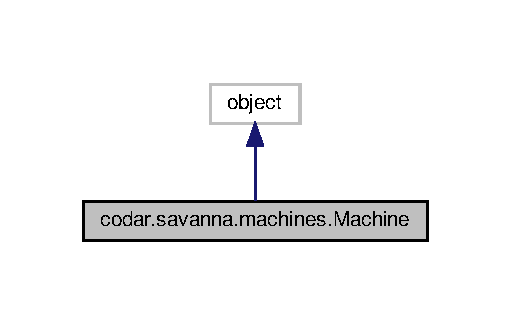
\includegraphics[width=245pt]{classcodar_1_1savanna_1_1machines_1_1_machine__inherit__graph}
\end{center}
\end{figure}


Collaboration diagram for codar.\+savanna.\+machines.\+Machine\+:
\nopagebreak
\begin{figure}[H]
\begin{center}
\leavevmode
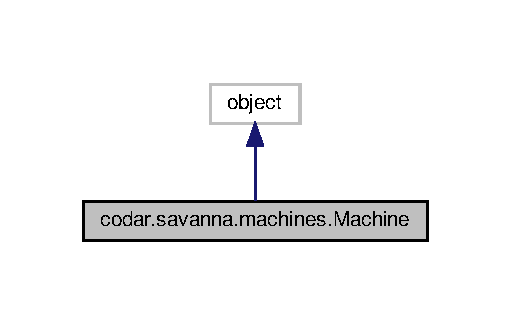
\includegraphics[width=245pt]{classcodar_1_1savanna_1_1machines_1_1_machine__coll__graph}
\end{center}
\end{figure}
\subsection*{Public Member Functions}
\begin{DoxyCompactItemize}
\item 
def \hyperlink{classcodar_1_1savanna_1_1machines_1_1_machine_a604279a4e666c75e59716eefc01be972}{\+\_\+\+\_\+init\+\_\+\+\_\+} (self, \hyperlink{classcodar_1_1savanna_1_1machines_1_1_machine_a7d2164c63e076a7240947b1a70e62f0f}{name}, \hyperlink{classcodar_1_1savanna_1_1machines_1_1_machine_a179ace208a51d849459bf26fcf54acc4}{scheduler\+\_\+name}, \hyperlink{classcodar_1_1savanna_1_1machines_1_1_machine_a65b17faeda10d83fdd8766430d62815f}{runner\+\_\+name}, \hyperlink{classcodar_1_1savanna_1_1machines_1_1_machine_ad1f413ae8607221317675adb19a7887a}{node\+\_\+class}, \hyperlink{classcodar_1_1savanna_1_1machines_1_1_machine_a4b4c0eda863f1003ae7d8bda02f2b96b}{processes\+\_\+per\+\_\+node}=None, \hyperlink{classcodar_1_1savanna_1_1machines_1_1_machine_a516048c489dc334f0fe45d529e59c181}{node\+\_\+exclusive}=False, \hyperlink{classcodar_1_1savanna_1_1machines_1_1_machine_aa26c50a13e89160894eff5a7fb180ed7}{scheduler\+\_\+options}=None, \hyperlink{classcodar_1_1savanna_1_1machines_1_1_machine_a636168243907ca1035c8683a31a69c86}{dataspaces\+\_\+servers\+\_\+per\+\_\+node}=1)
\item 
def \hyperlink{classcodar_1_1savanna_1_1machines_1_1_machine_a50a9259a741eef79d1de2529a9d1f1ae}{get\+\_\+scheduler\+\_\+options} (self, options)
\item 
def \hyperlink{classcodar_1_1savanna_1_1machines_1_1_machine_a13cd507ffb654ef95477f9cd22de6691}{get\+\_\+nodes\+\_\+reqd} (self)
\end{DoxyCompactItemize}
\subsection*{Public Attributes}
\begin{DoxyCompactItemize}
\item 
\hyperlink{classcodar_1_1savanna_1_1machines_1_1_machine_a7d2164c63e076a7240947b1a70e62f0f}{name}
\item 
\hyperlink{classcodar_1_1savanna_1_1machines_1_1_machine_a179ace208a51d849459bf26fcf54acc4}{scheduler\+\_\+name}
\item 
\hyperlink{classcodar_1_1savanna_1_1machines_1_1_machine_a65b17faeda10d83fdd8766430d62815f}{runner\+\_\+name}
\item 
\hyperlink{classcodar_1_1savanna_1_1machines_1_1_machine_ad1f413ae8607221317675adb19a7887a}{node\+\_\+class}
\item 
\hyperlink{classcodar_1_1savanna_1_1machines_1_1_machine_a4b4c0eda863f1003ae7d8bda02f2b96b}{processes\+\_\+per\+\_\+node}
\item 
\hyperlink{classcodar_1_1savanna_1_1machines_1_1_machine_a516048c489dc334f0fe45d529e59c181}{node\+\_\+exclusive}
\item 
\hyperlink{classcodar_1_1savanna_1_1machines_1_1_machine_aa26c50a13e89160894eff5a7fb180ed7}{scheduler\+\_\+options}
\item 
\hyperlink{classcodar_1_1savanna_1_1machines_1_1_machine_a636168243907ca1035c8683a31a69c86}{dataspaces\+\_\+servers\+\_\+per\+\_\+node}
\end{DoxyCompactItemize}


\subsection{Detailed Description}
\begin{DoxyVerb}Class to represent configuration of a specific Supercomputer or
workstation, including the scheduler and runner used by the machine.
This can be used to map an experiment to run on the machine without
having to define machine specific parameter for every experiment
separately.\end{DoxyVerb}
 

Definition at line 69 of file machines.\+py.



\subsection{Constructor \& Destructor Documentation}
\mbox{\Hypertarget{classcodar_1_1savanna_1_1machines_1_1_machine_a604279a4e666c75e59716eefc01be972}\label{classcodar_1_1savanna_1_1machines_1_1_machine_a604279a4e666c75e59716eefc01be972}} 
\index{codar\+::savanna\+::machines\+::\+Machine@{codar\+::savanna\+::machines\+::\+Machine}!\+\_\+\+\_\+init\+\_\+\+\_\+@{\+\_\+\+\_\+init\+\_\+\+\_\+}}
\index{\+\_\+\+\_\+init\+\_\+\+\_\+@{\+\_\+\+\_\+init\+\_\+\+\_\+}!codar\+::savanna\+::machines\+::\+Machine@{codar\+::savanna\+::machines\+::\+Machine}}
\subsubsection{\texorpdfstring{\+\_\+\+\_\+init\+\_\+\+\_\+()}{\_\_init\_\_()}}
{\footnotesize\ttfamily def codar.\+savanna.\+machines.\+Machine.\+\_\+\+\_\+init\+\_\+\+\_\+ (\begin{DoxyParamCaption}\item[{}]{self,  }\item[{}]{name,  }\item[{}]{scheduler\+\_\+name,  }\item[{}]{runner\+\_\+name,  }\item[{}]{node\+\_\+class,  }\item[{}]{processes\+\_\+per\+\_\+node = {\ttfamily None},  }\item[{}]{node\+\_\+exclusive = {\ttfamily False},  }\item[{}]{scheduler\+\_\+options = {\ttfamily None},  }\item[{}]{dataspaces\+\_\+servers\+\_\+per\+\_\+node = {\ttfamily 1} }\end{DoxyParamCaption})}



Definition at line 78 of file machines.\+py.



\subsection{Member Function Documentation}
\mbox{\Hypertarget{classcodar_1_1savanna_1_1machines_1_1_machine_a13cd507ffb654ef95477f9cd22de6691}\label{classcodar_1_1savanna_1_1machines_1_1_machine_a13cd507ffb654ef95477f9cd22de6691}} 
\index{codar\+::savanna\+::machines\+::\+Machine@{codar\+::savanna\+::machines\+::\+Machine}!get\+\_\+nodes\+\_\+reqd@{get\+\_\+nodes\+\_\+reqd}}
\index{get\+\_\+nodes\+\_\+reqd@{get\+\_\+nodes\+\_\+reqd}!codar\+::savanna\+::machines\+::\+Machine@{codar\+::savanna\+::machines\+::\+Machine}}
\subsubsection{\texorpdfstring{get\+\_\+nodes\+\_\+reqd()}{get\_nodes\_reqd()}}
{\footnotesize\ttfamily def codar.\+savanna.\+machines.\+Machine.\+get\+\_\+nodes\+\_\+reqd (\begin{DoxyParamCaption}\item[{}]{self }\end{DoxyParamCaption})}



Definition at line 100 of file machines.\+py.

\mbox{\Hypertarget{classcodar_1_1savanna_1_1machines_1_1_machine_a50a9259a741eef79d1de2529a9d1f1ae}\label{classcodar_1_1savanna_1_1machines_1_1_machine_a50a9259a741eef79d1de2529a9d1f1ae}} 
\index{codar\+::savanna\+::machines\+::\+Machine@{codar\+::savanna\+::machines\+::\+Machine}!get\+\_\+scheduler\+\_\+options@{get\+\_\+scheduler\+\_\+options}}
\index{get\+\_\+scheduler\+\_\+options@{get\+\_\+scheduler\+\_\+options}!codar\+::savanna\+::machines\+::\+Machine@{codar\+::savanna\+::machines\+::\+Machine}}
\subsubsection{\texorpdfstring{get\+\_\+scheduler\+\_\+options()}{get\_scheduler\_options()}}
{\footnotesize\ttfamily def codar.\+savanna.\+machines.\+Machine.\+get\+\_\+scheduler\+\_\+options (\begin{DoxyParamCaption}\item[{}]{self,  }\item[{}]{options }\end{DoxyParamCaption})}

\begin{DoxyVerb}Validate supplied options and add default values where missing.
Returns a new dictionary.\end{DoxyVerb}
 

Definition at line 91 of file machines.\+py.



\subsection{Member Data Documentation}
\mbox{\Hypertarget{classcodar_1_1savanna_1_1machines_1_1_machine_a636168243907ca1035c8683a31a69c86}\label{classcodar_1_1savanna_1_1machines_1_1_machine_a636168243907ca1035c8683a31a69c86}} 
\index{codar\+::savanna\+::machines\+::\+Machine@{codar\+::savanna\+::machines\+::\+Machine}!dataspaces\+\_\+servers\+\_\+per\+\_\+node@{dataspaces\+\_\+servers\+\_\+per\+\_\+node}}
\index{dataspaces\+\_\+servers\+\_\+per\+\_\+node@{dataspaces\+\_\+servers\+\_\+per\+\_\+node}!codar\+::savanna\+::machines\+::\+Machine@{codar\+::savanna\+::machines\+::\+Machine}}
\subsubsection{\texorpdfstring{dataspaces\+\_\+servers\+\_\+per\+\_\+node}{dataspaces\_servers\_per\_node}}
{\footnotesize\ttfamily codar.\+savanna.\+machines.\+Machine.\+dataspaces\+\_\+servers\+\_\+per\+\_\+node}



Definition at line 89 of file machines.\+py.

\mbox{\Hypertarget{classcodar_1_1savanna_1_1machines_1_1_machine_a7d2164c63e076a7240947b1a70e62f0f}\label{classcodar_1_1savanna_1_1machines_1_1_machine_a7d2164c63e076a7240947b1a70e62f0f}} 
\index{codar\+::savanna\+::machines\+::\+Machine@{codar\+::savanna\+::machines\+::\+Machine}!name@{name}}
\index{name@{name}!codar\+::savanna\+::machines\+::\+Machine@{codar\+::savanna\+::machines\+::\+Machine}}
\subsubsection{\texorpdfstring{name}{name}}
{\footnotesize\ttfamily codar.\+savanna.\+machines.\+Machine.\+name}



Definition at line 79 of file machines.\+py.

\mbox{\Hypertarget{classcodar_1_1savanna_1_1machines_1_1_machine_ad1f413ae8607221317675adb19a7887a}\label{classcodar_1_1savanna_1_1machines_1_1_machine_ad1f413ae8607221317675adb19a7887a}} 
\index{codar\+::savanna\+::machines\+::\+Machine@{codar\+::savanna\+::machines\+::\+Machine}!node\+\_\+class@{node\+\_\+class}}
\index{node\+\_\+class@{node\+\_\+class}!codar\+::savanna\+::machines\+::\+Machine@{codar\+::savanna\+::machines\+::\+Machine}}
\subsubsection{\texorpdfstring{node\+\_\+class}{node\_class}}
{\footnotesize\ttfamily codar.\+savanna.\+machines.\+Machine.\+node\+\_\+class}



Definition at line 82 of file machines.\+py.

\mbox{\Hypertarget{classcodar_1_1savanna_1_1machines_1_1_machine_a516048c489dc334f0fe45d529e59c181}\label{classcodar_1_1savanna_1_1machines_1_1_machine_a516048c489dc334f0fe45d529e59c181}} 
\index{codar\+::savanna\+::machines\+::\+Machine@{codar\+::savanna\+::machines\+::\+Machine}!node\+\_\+exclusive@{node\+\_\+exclusive}}
\index{node\+\_\+exclusive@{node\+\_\+exclusive}!codar\+::savanna\+::machines\+::\+Machine@{codar\+::savanna\+::machines\+::\+Machine}}
\subsubsection{\texorpdfstring{node\+\_\+exclusive}{node\_exclusive}}
{\footnotesize\ttfamily codar.\+savanna.\+machines.\+Machine.\+node\+\_\+exclusive}



Definition at line 86 of file machines.\+py.

\mbox{\Hypertarget{classcodar_1_1savanna_1_1machines_1_1_machine_a4b4c0eda863f1003ae7d8bda02f2b96b}\label{classcodar_1_1savanna_1_1machines_1_1_machine_a4b4c0eda863f1003ae7d8bda02f2b96b}} 
\index{codar\+::savanna\+::machines\+::\+Machine@{codar\+::savanna\+::machines\+::\+Machine}!processes\+\_\+per\+\_\+node@{processes\+\_\+per\+\_\+node}}
\index{processes\+\_\+per\+\_\+node@{processes\+\_\+per\+\_\+node}!codar\+::savanna\+::machines\+::\+Machine@{codar\+::savanna\+::machines\+::\+Machine}}
\subsubsection{\texorpdfstring{processes\+\_\+per\+\_\+node}{processes\_per\_node}}
{\footnotesize\ttfamily codar.\+savanna.\+machines.\+Machine.\+processes\+\_\+per\+\_\+node}



Definition at line 85 of file machines.\+py.

\mbox{\Hypertarget{classcodar_1_1savanna_1_1machines_1_1_machine_a65b17faeda10d83fdd8766430d62815f}\label{classcodar_1_1savanna_1_1machines_1_1_machine_a65b17faeda10d83fdd8766430d62815f}} 
\index{codar\+::savanna\+::machines\+::\+Machine@{codar\+::savanna\+::machines\+::\+Machine}!runner\+\_\+name@{runner\+\_\+name}}
\index{runner\+\_\+name@{runner\+\_\+name}!codar\+::savanna\+::machines\+::\+Machine@{codar\+::savanna\+::machines\+::\+Machine}}
\subsubsection{\texorpdfstring{runner\+\_\+name}{runner\_name}}
{\footnotesize\ttfamily codar.\+savanna.\+machines.\+Machine.\+runner\+\_\+name}



Definition at line 81 of file machines.\+py.

\mbox{\Hypertarget{classcodar_1_1savanna_1_1machines_1_1_machine_a179ace208a51d849459bf26fcf54acc4}\label{classcodar_1_1savanna_1_1machines_1_1_machine_a179ace208a51d849459bf26fcf54acc4}} 
\index{codar\+::savanna\+::machines\+::\+Machine@{codar\+::savanna\+::machines\+::\+Machine}!scheduler\+\_\+name@{scheduler\+\_\+name}}
\index{scheduler\+\_\+name@{scheduler\+\_\+name}!codar\+::savanna\+::machines\+::\+Machine@{codar\+::savanna\+::machines\+::\+Machine}}
\subsubsection{\texorpdfstring{scheduler\+\_\+name}{scheduler\_name}}
{\footnotesize\ttfamily codar.\+savanna.\+machines.\+Machine.\+scheduler\+\_\+name}



Definition at line 80 of file machines.\+py.

\mbox{\Hypertarget{classcodar_1_1savanna_1_1machines_1_1_machine_aa26c50a13e89160894eff5a7fb180ed7}\label{classcodar_1_1savanna_1_1machines_1_1_machine_aa26c50a13e89160894eff5a7fb180ed7}} 
\index{codar\+::savanna\+::machines\+::\+Machine@{codar\+::savanna\+::machines\+::\+Machine}!scheduler\+\_\+options@{scheduler\+\_\+options}}
\index{scheduler\+\_\+options@{scheduler\+\_\+options}!codar\+::savanna\+::machines\+::\+Machine@{codar\+::savanna\+::machines\+::\+Machine}}
\subsubsection{\texorpdfstring{scheduler\+\_\+options}{scheduler\_options}}
{\footnotesize\ttfamily codar.\+savanna.\+machines.\+Machine.\+scheduler\+\_\+options}



Definition at line 88 of file machines.\+py.



The documentation for this class was generated from the following file\+:\begin{DoxyCompactItemize}
\item 
savanna/\hyperlink{machines_8py}{machines.\+py}\end{DoxyCompactItemize}

\hypertarget{classcodar_1_1savanna_1_1machines_1_1_machine_node}{}\section{codar.\+savanna.\+machines.\+Machine\+Node Class Reference}
\label{classcodar_1_1savanna_1_1machines_1_1_machine_node}\index{codar.\+savanna.\+machines.\+Machine\+Node@{codar.\+savanna.\+machines.\+Machine\+Node}}


Inheritance diagram for codar.\+savanna.\+machines.\+Machine\+Node\+:
\nopagebreak
\begin{figure}[H]
\begin{center}
\leavevmode
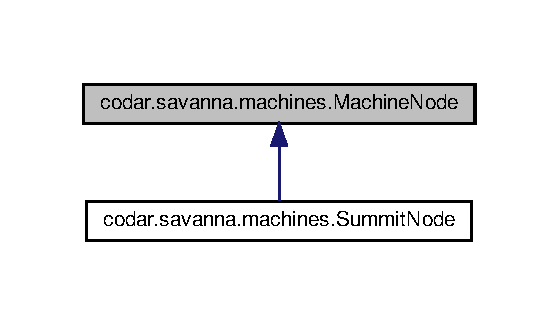
\includegraphics[width=268pt]{classcodar_1_1savanna_1_1machines_1_1_machine_node__inherit__graph}
\end{center}
\end{figure}
\subsection*{Public Member Functions}
\begin{DoxyCompactItemize}
\item 
def \hyperlink{classcodar_1_1savanna_1_1machines_1_1_machine_node_adc12f9810d54e9f497a4df2c3ab80577}{\+\_\+\+\_\+init\+\_\+\+\_\+} (self, num\+\_\+cpus, num\+\_\+gpus)
\item 
def \hyperlink{classcodar_1_1savanna_1_1machines_1_1_machine_node_a32ee6eb242c8dff720e89ffbd772cf40}{validate\+\_\+layout} (self)
\item 
def \hyperlink{classcodar_1_1savanna_1_1machines_1_1_machine_node_a9598980dfb90152c1f2091fae5dd1299}{to\+\_\+json} (self)
\end{DoxyCompactItemize}
\subsection*{Public Attributes}
\begin{DoxyCompactItemize}
\item 
\hyperlink{classcodar_1_1savanna_1_1machines_1_1_machine_node_a084bb8daed740edd8b7dd37f8d1f9bab}{cpu}
\item 
\hyperlink{classcodar_1_1savanna_1_1machines_1_1_machine_node_a2ccec1288c1472fc0a5af7787e48da22}{gpu}
\end{DoxyCompactItemize}


\subsection{Detailed Description}


Definition at line 16 of file machines.\+py.



\subsection{Constructor \& Destructor Documentation}
\mbox{\Hypertarget{classcodar_1_1savanna_1_1machines_1_1_machine_node_adc12f9810d54e9f497a4df2c3ab80577}\label{classcodar_1_1savanna_1_1machines_1_1_machine_node_adc12f9810d54e9f497a4df2c3ab80577}} 
\index{codar\+::savanna\+::machines\+::\+Machine\+Node@{codar\+::savanna\+::machines\+::\+Machine\+Node}!\+\_\+\+\_\+init\+\_\+\+\_\+@{\+\_\+\+\_\+init\+\_\+\+\_\+}}
\index{\+\_\+\+\_\+init\+\_\+\+\_\+@{\+\_\+\+\_\+init\+\_\+\+\_\+}!codar\+::savanna\+::machines\+::\+Machine\+Node@{codar\+::savanna\+::machines\+::\+Machine\+Node}}
\subsubsection{\texorpdfstring{\+\_\+\+\_\+init\+\_\+\+\_\+()}{\_\_init\_\_()}}
{\footnotesize\ttfamily def codar.\+savanna.\+machines.\+Machine\+Node.\+\_\+\+\_\+init\+\_\+\+\_\+ (\begin{DoxyParamCaption}\item[{}]{self,  }\item[{}]{num\+\_\+cpus,  }\item[{}]{num\+\_\+gpus }\end{DoxyParamCaption})}



Definition at line 17 of file machines.\+py.



\subsection{Member Function Documentation}
\mbox{\Hypertarget{classcodar_1_1savanna_1_1machines_1_1_machine_node_a9598980dfb90152c1f2091fae5dd1299}\label{classcodar_1_1savanna_1_1machines_1_1_machine_node_a9598980dfb90152c1f2091fae5dd1299}} 
\index{codar\+::savanna\+::machines\+::\+Machine\+Node@{codar\+::savanna\+::machines\+::\+Machine\+Node}!to\+\_\+json@{to\+\_\+json}}
\index{to\+\_\+json@{to\+\_\+json}!codar\+::savanna\+::machines\+::\+Machine\+Node@{codar\+::savanna\+::machines\+::\+Machine\+Node}}
\subsubsection{\texorpdfstring{to\+\_\+json()}{to\_json()}}
{\footnotesize\ttfamily def codar.\+savanna.\+machines.\+Machine\+Node.\+to\+\_\+json (\begin{DoxyParamCaption}\item[{}]{self }\end{DoxyParamCaption})}



Definition at line 25 of file machines.\+py.

\mbox{\Hypertarget{classcodar_1_1savanna_1_1machines_1_1_machine_node_a32ee6eb242c8dff720e89ffbd772cf40}\label{classcodar_1_1savanna_1_1machines_1_1_machine_node_a32ee6eb242c8dff720e89ffbd772cf40}} 
\index{codar\+::savanna\+::machines\+::\+Machine\+Node@{codar\+::savanna\+::machines\+::\+Machine\+Node}!validate\+\_\+layout@{validate\+\_\+layout}}
\index{validate\+\_\+layout@{validate\+\_\+layout}!codar\+::savanna\+::machines\+::\+Machine\+Node@{codar\+::savanna\+::machines\+::\+Machine\+Node}}
\subsubsection{\texorpdfstring{validate\+\_\+layout()}{validate\_layout()}}
{\footnotesize\ttfamily def codar.\+savanna.\+machines.\+Machine\+Node.\+validate\+\_\+layout (\begin{DoxyParamCaption}\item[{}]{self }\end{DoxyParamCaption})}



Definition at line 22 of file machines.\+py.



\subsection{Member Data Documentation}
\mbox{\Hypertarget{classcodar_1_1savanna_1_1machines_1_1_machine_node_a084bb8daed740edd8b7dd37f8d1f9bab}\label{classcodar_1_1savanna_1_1machines_1_1_machine_node_a084bb8daed740edd8b7dd37f8d1f9bab}} 
\index{codar\+::savanna\+::machines\+::\+Machine\+Node@{codar\+::savanna\+::machines\+::\+Machine\+Node}!cpu@{cpu}}
\index{cpu@{cpu}!codar\+::savanna\+::machines\+::\+Machine\+Node@{codar\+::savanna\+::machines\+::\+Machine\+Node}}
\subsubsection{\texorpdfstring{cpu}{cpu}}
{\footnotesize\ttfamily codar.\+savanna.\+machines.\+Machine\+Node.\+cpu}



Definition at line 19 of file machines.\+py.

\mbox{\Hypertarget{classcodar_1_1savanna_1_1machines_1_1_machine_node_a2ccec1288c1472fc0a5af7787e48da22}\label{classcodar_1_1savanna_1_1machines_1_1_machine_node_a2ccec1288c1472fc0a5af7787e48da22}} 
\index{codar\+::savanna\+::machines\+::\+Machine\+Node@{codar\+::savanna\+::machines\+::\+Machine\+Node}!gpu@{gpu}}
\index{gpu@{gpu}!codar\+::savanna\+::machines\+::\+Machine\+Node@{codar\+::savanna\+::machines\+::\+Machine\+Node}}
\subsubsection{\texorpdfstring{gpu}{gpu}}
{\footnotesize\ttfamily codar.\+savanna.\+machines.\+Machine\+Node.\+gpu}



Definition at line 20 of file machines.\+py.



The documentation for this class was generated from the following file\+:\begin{DoxyCompactItemize}
\item 
savanna/\hyperlink{machines_8py}{machines.\+py}\end{DoxyCompactItemize}

\hypertarget{classcodar_1_1savanna_1_1exc_1_1_machine_not_found}{}\section{codar.\+savanna.\+exc.\+Machine\+Not\+Found Class Reference}
\label{classcodar_1_1savanna_1_1exc_1_1_machine_not_found}\index{codar.\+savanna.\+exc.\+Machine\+Not\+Found@{codar.\+savanna.\+exc.\+Machine\+Not\+Found}}


Inheritance diagram for codar.\+savanna.\+exc.\+Machine\+Not\+Found\+:
\nopagebreak
\begin{figure}[H]
\begin{center}
\leavevmode
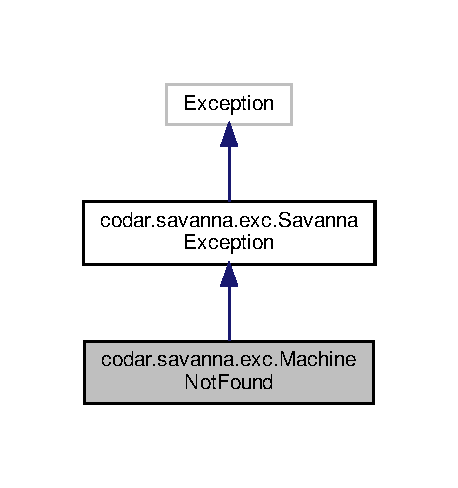
\includegraphics[width=220pt]{classcodar_1_1savanna_1_1exc_1_1_machine_not_found__inherit__graph}
\end{center}
\end{figure}


Collaboration diagram for codar.\+savanna.\+exc.\+Machine\+Not\+Found\+:
\nopagebreak
\begin{figure}[H]
\begin{center}
\leavevmode
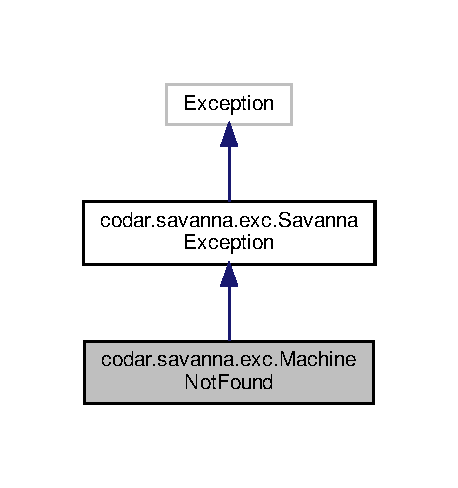
\includegraphics[width=220pt]{classcodar_1_1savanna_1_1exc_1_1_machine_not_found__coll__graph}
\end{center}
\end{figure}
\subsection*{Public Member Functions}
\begin{DoxyCompactItemize}
\item 
def \hyperlink{classcodar_1_1savanna_1_1exc_1_1_machine_not_found_aac59d9a2636166df83d3260fb7bc8933}{\+\_\+\+\_\+init\+\_\+\+\_\+} (self, machine\+\_\+name)
\end{DoxyCompactItemize}


\subsection{Detailed Description}


Definition at line 10 of file exc.\+py.



\subsection{Constructor \& Destructor Documentation}
\mbox{\Hypertarget{classcodar_1_1savanna_1_1exc_1_1_machine_not_found_aac59d9a2636166df83d3260fb7bc8933}\label{classcodar_1_1savanna_1_1exc_1_1_machine_not_found_aac59d9a2636166df83d3260fb7bc8933}} 
\index{codar\+::savanna\+::exc\+::\+Machine\+Not\+Found@{codar\+::savanna\+::exc\+::\+Machine\+Not\+Found}!\+\_\+\+\_\+init\+\_\+\+\_\+@{\+\_\+\+\_\+init\+\_\+\+\_\+}}
\index{\+\_\+\+\_\+init\+\_\+\+\_\+@{\+\_\+\+\_\+init\+\_\+\+\_\+}!codar\+::savanna\+::exc\+::\+Machine\+Not\+Found@{codar\+::savanna\+::exc\+::\+Machine\+Not\+Found}}
\subsubsection{\texorpdfstring{\+\_\+\+\_\+init\+\_\+\+\_\+()}{\_\_init\_\_()}}
{\footnotesize\ttfamily def codar.\+savanna.\+exc.\+Machine\+Not\+Found.\+\_\+\+\_\+init\+\_\+\+\_\+ (\begin{DoxyParamCaption}\item[{}]{self,  }\item[{}]{machine\+\_\+name }\end{DoxyParamCaption})}



Definition at line 11 of file exc.\+py.



The documentation for this class was generated from the following file\+:\begin{DoxyCompactItemize}
\item 
\hyperlink{exc_8py}{exc.\+py}\end{DoxyCompactItemize}

\hypertarget{classcodar_1_1cheetah_1_1exc_1_1_machine_not_found}{}\section{codar.\+cheetah.\+exc.\+Machine\+Not\+Found Class Reference}
\label{classcodar_1_1cheetah_1_1exc_1_1_machine_not_found}\index{codar.\+cheetah.\+exc.\+Machine\+Not\+Found@{codar.\+cheetah.\+exc.\+Machine\+Not\+Found}}


Inheritance diagram for codar.\+cheetah.\+exc.\+Machine\+Not\+Found\+:
\nopagebreak
\begin{figure}[H]
\begin{center}
\leavevmode
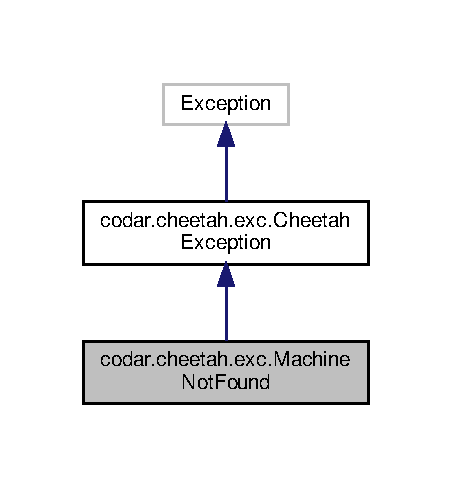
\includegraphics[width=217pt]{classcodar_1_1cheetah_1_1exc_1_1_machine_not_found__inherit__graph}
\end{center}
\end{figure}


Collaboration diagram for codar.\+cheetah.\+exc.\+Machine\+Not\+Found\+:
\nopagebreak
\begin{figure}[H]
\begin{center}
\leavevmode
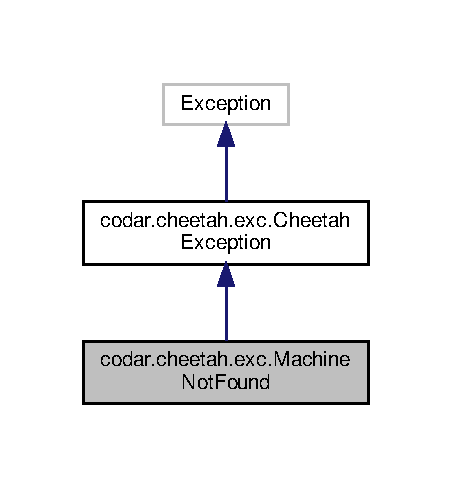
\includegraphics[width=217pt]{classcodar_1_1cheetah_1_1exc_1_1_machine_not_found__coll__graph}
\end{center}
\end{figure}
\subsection*{Public Member Functions}
\begin{DoxyCompactItemize}
\item 
\mbox{\Hypertarget{classcodar_1_1cheetah_1_1exc_1_1_machine_not_found_ae688c3fce79910a0bd7cd1e553be32cf}\label{classcodar_1_1cheetah_1_1exc_1_1_machine_not_found_ae688c3fce79910a0bd7cd1e553be32cf}} 
def {\bfseries \+\_\+\+\_\+init\+\_\+\+\_\+} (self, machine\+\_\+name)
\end{DoxyCompactItemize}


The documentation for this class was generated from the following file\+:\begin{DoxyCompactItemize}
\item 
exc.\+py\end{DoxyCompactItemize}

\hypertarget{classcodar_1_1savanna_1_1runners_1_1_m_p_i_runner}{}\section{codar.\+savanna.\+runners.\+M\+P\+I\+Runner Class Reference}
\label{classcodar_1_1savanna_1_1runners_1_1_m_p_i_runner}\index{codar.\+savanna.\+runners.\+M\+P\+I\+Runner@{codar.\+savanna.\+runners.\+M\+P\+I\+Runner}}


Inheritance diagram for codar.\+savanna.\+runners.\+M\+P\+I\+Runner\+:
\nopagebreak
\begin{figure}[H]
\begin{center}
\leavevmode
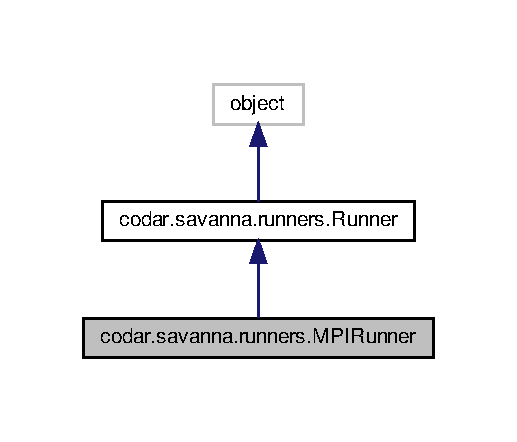
\includegraphics[width=248pt]{classcodar_1_1savanna_1_1runners_1_1_m_p_i_runner__inherit__graph}
\end{center}
\end{figure}


Collaboration diagram for codar.\+savanna.\+runners.\+M\+P\+I\+Runner\+:
\nopagebreak
\begin{figure}[H]
\begin{center}
\leavevmode
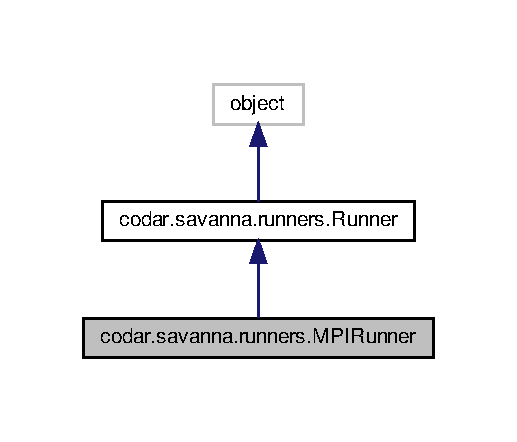
\includegraphics[width=248pt]{classcodar_1_1savanna_1_1runners_1_1_m_p_i_runner__coll__graph}
\end{center}
\end{figure}
\subsection*{Public Member Functions}
\begin{DoxyCompactItemize}
\item 
def \hyperlink{classcodar_1_1savanna_1_1runners_1_1_m_p_i_runner_a67662602e1fe9901e20e17a9f16b8259}{\+\_\+\+\_\+init\+\_\+\+\_\+} (self, \hyperlink{classcodar_1_1savanna_1_1runners_1_1_m_p_i_runner_a7ccd767eb30cbd555f387e5b4d781ffa}{exe}, \hyperlink{classcodar_1_1savanna_1_1runners_1_1_m_p_i_runner_aafcba954932f2160d43e820cf3abe6e1}{nprocs\+\_\+arg}, \hyperlink{classcodar_1_1savanna_1_1runners_1_1_m_p_i_runner_ad139718b16183bd45520e166d6d2b9b9}{nodes\+\_\+arg}=None, \hyperlink{classcodar_1_1savanna_1_1runners_1_1_m_p_i_runner_a58bd05be3e876f5a8f2522262ba934f7}{tasks\+\_\+per\+\_\+node\+\_\+arg}=None, \hyperlink{classcodar_1_1savanna_1_1runners_1_1_m_p_i_runner_ad36885eab0821c149e8798ffbf567af4}{hostfile}=None)
\item 
def \hyperlink{classcodar_1_1savanna_1_1runners_1_1_m_p_i_runner_a2eb86e6b8495ecf2361dc58e4b05c7c5}{wrap} (self, run, sched\+\_\+args, find\+\_\+in\+\_\+path=True)
\end{DoxyCompactItemize}
\subsection*{Public Attributes}
\begin{DoxyCompactItemize}
\item 
\hyperlink{classcodar_1_1savanna_1_1runners_1_1_m_p_i_runner_a7ccd767eb30cbd555f387e5b4d781ffa}{exe}
\item 
\hyperlink{classcodar_1_1savanna_1_1runners_1_1_m_p_i_runner_aafcba954932f2160d43e820cf3abe6e1}{nprocs\+\_\+arg}
\item 
\hyperlink{classcodar_1_1savanna_1_1runners_1_1_m_p_i_runner_ad139718b16183bd45520e166d6d2b9b9}{nodes\+\_\+arg}
\item 
\hyperlink{classcodar_1_1savanna_1_1runners_1_1_m_p_i_runner_a58bd05be3e876f5a8f2522262ba934f7}{tasks\+\_\+per\+\_\+node\+\_\+arg}
\item 
\hyperlink{classcodar_1_1savanna_1_1runners_1_1_m_p_i_runner_ad36885eab0821c149e8798ffbf567af4}{hostfile}
\end{DoxyCompactItemize}


\subsection{Detailed Description}


Definition at line 11 of file runners.\+py.



\subsection{Constructor \& Destructor Documentation}
\mbox{\Hypertarget{classcodar_1_1savanna_1_1runners_1_1_m_p_i_runner_a67662602e1fe9901e20e17a9f16b8259}\label{classcodar_1_1savanna_1_1runners_1_1_m_p_i_runner_a67662602e1fe9901e20e17a9f16b8259}} 
\index{codar\+::savanna\+::runners\+::\+M\+P\+I\+Runner@{codar\+::savanna\+::runners\+::\+M\+P\+I\+Runner}!\+\_\+\+\_\+init\+\_\+\+\_\+@{\+\_\+\+\_\+init\+\_\+\+\_\+}}
\index{\+\_\+\+\_\+init\+\_\+\+\_\+@{\+\_\+\+\_\+init\+\_\+\+\_\+}!codar\+::savanna\+::runners\+::\+M\+P\+I\+Runner@{codar\+::savanna\+::runners\+::\+M\+P\+I\+Runner}}
\subsubsection{\texorpdfstring{\+\_\+\+\_\+init\+\_\+\+\_\+()}{\_\_init\_\_()}}
{\footnotesize\ttfamily def codar.\+savanna.\+runners.\+M\+P\+I\+Runner.\+\_\+\+\_\+init\+\_\+\+\_\+ (\begin{DoxyParamCaption}\item[{}]{self,  }\item[{}]{exe,  }\item[{}]{nprocs\+\_\+arg,  }\item[{}]{nodes\+\_\+arg = {\ttfamily None},  }\item[{}]{tasks\+\_\+per\+\_\+node\+\_\+arg = {\ttfamily None},  }\item[{}]{hostfile = {\ttfamily None} }\end{DoxyParamCaption})}



Definition at line 13 of file runners.\+py.



\subsection{Member Function Documentation}
\mbox{\Hypertarget{classcodar_1_1savanna_1_1runners_1_1_m_p_i_runner_a2eb86e6b8495ecf2361dc58e4b05c7c5}\label{classcodar_1_1savanna_1_1runners_1_1_m_p_i_runner_a2eb86e6b8495ecf2361dc58e4b05c7c5}} 
\index{codar\+::savanna\+::runners\+::\+M\+P\+I\+Runner@{codar\+::savanna\+::runners\+::\+M\+P\+I\+Runner}!wrap@{wrap}}
\index{wrap@{wrap}!codar\+::savanna\+::runners\+::\+M\+P\+I\+Runner@{codar\+::savanna\+::runners\+::\+M\+P\+I\+Runner}}
\subsubsection{\texorpdfstring{wrap()}{wrap()}}
{\footnotesize\ttfamily def codar.\+savanna.\+runners.\+M\+P\+I\+Runner.\+wrap (\begin{DoxyParamCaption}\item[{}]{self,  }\item[{}]{run,  }\item[{}]{sched\+\_\+args,  }\item[{}]{find\+\_\+in\+\_\+path = {\ttfamily True} }\end{DoxyParamCaption})}



Definition at line 20 of file runners.\+py.



\subsection{Member Data Documentation}
\mbox{\Hypertarget{classcodar_1_1savanna_1_1runners_1_1_m_p_i_runner_a7ccd767eb30cbd555f387e5b4d781ffa}\label{classcodar_1_1savanna_1_1runners_1_1_m_p_i_runner_a7ccd767eb30cbd555f387e5b4d781ffa}} 
\index{codar\+::savanna\+::runners\+::\+M\+P\+I\+Runner@{codar\+::savanna\+::runners\+::\+M\+P\+I\+Runner}!exe@{exe}}
\index{exe@{exe}!codar\+::savanna\+::runners\+::\+M\+P\+I\+Runner@{codar\+::savanna\+::runners\+::\+M\+P\+I\+Runner}}
\subsubsection{\texorpdfstring{exe}{exe}}
{\footnotesize\ttfamily codar.\+savanna.\+runners.\+M\+P\+I\+Runner.\+exe}



Definition at line 14 of file runners.\+py.

\mbox{\Hypertarget{classcodar_1_1savanna_1_1runners_1_1_m_p_i_runner_ad36885eab0821c149e8798ffbf567af4}\label{classcodar_1_1savanna_1_1runners_1_1_m_p_i_runner_ad36885eab0821c149e8798ffbf567af4}} 
\index{codar\+::savanna\+::runners\+::\+M\+P\+I\+Runner@{codar\+::savanna\+::runners\+::\+M\+P\+I\+Runner}!hostfile@{hostfile}}
\index{hostfile@{hostfile}!codar\+::savanna\+::runners\+::\+M\+P\+I\+Runner@{codar\+::savanna\+::runners\+::\+M\+P\+I\+Runner}}
\subsubsection{\texorpdfstring{hostfile}{hostfile}}
{\footnotesize\ttfamily codar.\+savanna.\+runners.\+M\+P\+I\+Runner.\+hostfile}



Definition at line 18 of file runners.\+py.

\mbox{\Hypertarget{classcodar_1_1savanna_1_1runners_1_1_m_p_i_runner_ad139718b16183bd45520e166d6d2b9b9}\label{classcodar_1_1savanna_1_1runners_1_1_m_p_i_runner_ad139718b16183bd45520e166d6d2b9b9}} 
\index{codar\+::savanna\+::runners\+::\+M\+P\+I\+Runner@{codar\+::savanna\+::runners\+::\+M\+P\+I\+Runner}!nodes\+\_\+arg@{nodes\+\_\+arg}}
\index{nodes\+\_\+arg@{nodes\+\_\+arg}!codar\+::savanna\+::runners\+::\+M\+P\+I\+Runner@{codar\+::savanna\+::runners\+::\+M\+P\+I\+Runner}}
\subsubsection{\texorpdfstring{nodes\+\_\+arg}{nodes\_arg}}
{\footnotesize\ttfamily codar.\+savanna.\+runners.\+M\+P\+I\+Runner.\+nodes\+\_\+arg}



Definition at line 16 of file runners.\+py.

\mbox{\Hypertarget{classcodar_1_1savanna_1_1runners_1_1_m_p_i_runner_aafcba954932f2160d43e820cf3abe6e1}\label{classcodar_1_1savanna_1_1runners_1_1_m_p_i_runner_aafcba954932f2160d43e820cf3abe6e1}} 
\index{codar\+::savanna\+::runners\+::\+M\+P\+I\+Runner@{codar\+::savanna\+::runners\+::\+M\+P\+I\+Runner}!nprocs\+\_\+arg@{nprocs\+\_\+arg}}
\index{nprocs\+\_\+arg@{nprocs\+\_\+arg}!codar\+::savanna\+::runners\+::\+M\+P\+I\+Runner@{codar\+::savanna\+::runners\+::\+M\+P\+I\+Runner}}
\subsubsection{\texorpdfstring{nprocs\+\_\+arg}{nprocs\_arg}}
{\footnotesize\ttfamily codar.\+savanna.\+runners.\+M\+P\+I\+Runner.\+nprocs\+\_\+arg}



Definition at line 15 of file runners.\+py.

\mbox{\Hypertarget{classcodar_1_1savanna_1_1runners_1_1_m_p_i_runner_a58bd05be3e876f5a8f2522262ba934f7}\label{classcodar_1_1savanna_1_1runners_1_1_m_p_i_runner_a58bd05be3e876f5a8f2522262ba934f7}} 
\index{codar\+::savanna\+::runners\+::\+M\+P\+I\+Runner@{codar\+::savanna\+::runners\+::\+M\+P\+I\+Runner}!tasks\+\_\+per\+\_\+node\+\_\+arg@{tasks\+\_\+per\+\_\+node\+\_\+arg}}
\index{tasks\+\_\+per\+\_\+node\+\_\+arg@{tasks\+\_\+per\+\_\+node\+\_\+arg}!codar\+::savanna\+::runners\+::\+M\+P\+I\+Runner@{codar\+::savanna\+::runners\+::\+M\+P\+I\+Runner}}
\subsubsection{\texorpdfstring{tasks\+\_\+per\+\_\+node\+\_\+arg}{tasks\_per\_node\_arg}}
{\footnotesize\ttfamily codar.\+savanna.\+runners.\+M\+P\+I\+Runner.\+tasks\+\_\+per\+\_\+node\+\_\+arg}



Definition at line 17 of file runners.\+py.



The documentation for this class was generated from the following file\+:\begin{DoxyCompactItemize}
\item 
savanna/\hyperlink{savanna_2runners_8py}{runners.\+py}\end{DoxyCompactItemize}

\hypertarget{classcodar_1_1savanna_1_1model_1_1_node_config}{}\section{codar.\+savanna.\+model.\+Node\+Config Class Reference}
\label{classcodar_1_1savanna_1_1model_1_1_node_config}\index{codar.\+savanna.\+model.\+Node\+Config@{codar.\+savanna.\+model.\+Node\+Config}}
\subsection*{Public Member Functions}
\begin{DoxyCompactItemize}
\item 
def \hyperlink{classcodar_1_1savanna_1_1model_1_1_node_config_ad1fad3d3d97b1683dd4d28f77836a002}{\+\_\+\+\_\+init\+\_\+\+\_\+} (self)
\end{DoxyCompactItemize}
\subsection*{Public Attributes}
\begin{DoxyCompactItemize}
\item 
\mbox{\Hypertarget{classcodar_1_1savanna_1_1model_1_1_node_config_abfaac776b1cc5d4b0e6b3dd9d57a32be}\label{classcodar_1_1savanna_1_1model_1_1_node_config_abfaac776b1cc5d4b0e6b3dd9d57a32be}} 
{\bfseries num\+\_\+ranks\+\_\+per\+\_\+node}
\item 
\mbox{\Hypertarget{classcodar_1_1savanna_1_1model_1_1_node_config_ae3b3d48cf476cc01128973780c9ca256}\label{classcodar_1_1savanna_1_1model_1_1_node_config_ae3b3d48cf476cc01128973780c9ca256}} 
{\bfseries cpu}
\item 
\mbox{\Hypertarget{classcodar_1_1savanna_1_1model_1_1_node_config_a073c4acfc108df407fbd8ce570bade6b}\label{classcodar_1_1savanna_1_1model_1_1_node_config_a073c4acfc108df407fbd8ce570bade6b}} 
{\bfseries gpu}
\end{DoxyCompactItemize}


\subsection{Constructor \& Destructor Documentation}
\mbox{\Hypertarget{classcodar_1_1savanna_1_1model_1_1_node_config_ad1fad3d3d97b1683dd4d28f77836a002}\label{classcodar_1_1savanna_1_1model_1_1_node_config_ad1fad3d3d97b1683dd4d28f77836a002}} 
\index{codar\+::savanna\+::model\+::\+Node\+Config@{codar\+::savanna\+::model\+::\+Node\+Config}!\+\_\+\+\_\+init\+\_\+\+\_\+@{\+\_\+\+\_\+init\+\_\+\+\_\+}}
\index{\+\_\+\+\_\+init\+\_\+\+\_\+@{\+\_\+\+\_\+init\+\_\+\+\_\+}!codar\+::savanna\+::model\+::\+Node\+Config@{codar\+::savanna\+::model\+::\+Node\+Config}}
\subsubsection{\texorpdfstring{\+\_\+\+\_\+init\+\_\+\+\_\+()}{\_\_init\_\_()}}
{\footnotesize\ttfamily def codar.\+savanna.\+model.\+Node\+Config.\+\_\+\+\_\+init\+\_\+\+\_\+ (\begin{DoxyParamCaption}\item[{}]{self }\end{DoxyParamCaption})}

\begin{DoxyVerb}Intended to look like
cpu = [ 0=[], 1=[], 2=[], 3=[] ]
gpu = [ 0=[], 1=[], 2=[], 3=[] ]
\end{DoxyVerb}
 

The documentation for this class was generated from the following file\+:\begin{DoxyCompactItemize}
\item 
model.\+py\end{DoxyCompactItemize}

\hypertarget{classcodar_1_1savanna_1_1node__layout_1_1_node_layout}{}\section{codar.\+savanna.\+node\+\_\+layout.\+Node\+Layout Class Reference}
\label{classcodar_1_1savanna_1_1node__layout_1_1_node_layout}\index{codar.\+savanna.\+node\+\_\+layout.\+Node\+Layout@{codar.\+savanna.\+node\+\_\+layout.\+Node\+Layout}}


Inheritance diagram for codar.\+savanna.\+node\+\_\+layout.\+Node\+Layout\+:
\nopagebreak
\begin{figure}[H]
\begin{center}
\leavevmode
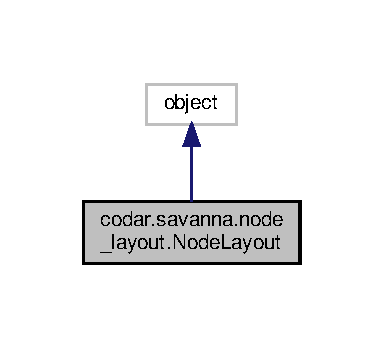
\includegraphics[width=184pt]{classcodar_1_1savanna_1_1node__layout_1_1_node_layout__inherit__graph}
\end{center}
\end{figure}


Collaboration diagram for codar.\+savanna.\+node\+\_\+layout.\+Node\+Layout\+:
\nopagebreak
\begin{figure}[H]
\begin{center}
\leavevmode
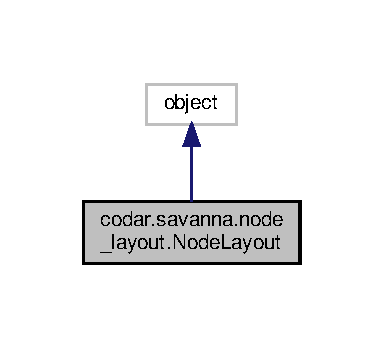
\includegraphics[width=184pt]{classcodar_1_1savanna_1_1node__layout_1_1_node_layout__coll__graph}
\end{center}
\end{figure}
\subsection*{Public Member Functions}
\begin{DoxyCompactItemize}
\item 
def \hyperlink{classcodar_1_1savanna_1_1node__layout_1_1_node_layout_af898ee59a1a5f520328a53d3b60a62d0}{\+\_\+\+\_\+init\+\_\+\+\_\+} (self, \hyperlink{classcodar_1_1savanna_1_1node__layout_1_1_node_layout_af27f209b198b9491d57d2bb3e65abc34}{layout\+\_\+list})
\item 
def \hyperlink{classcodar_1_1savanna_1_1node__layout_1_1_node_layout_ab0b94ca4a741efab71db5a598a782c38}{add\+\_\+node} (self, node\+\_\+dict)
\item 
def \hyperlink{classcodar_1_1savanna_1_1node__layout_1_1_node_layout_ae63a2f3c26294b78b35af77af4063899}{get\+\_\+node\+\_\+containing\+\_\+code} (self, code)
\item 
def \hyperlink{classcodar_1_1savanna_1_1node__layout_1_1_node_layout_add6c0879f2b8995f83cf07aaa09b7bbf}{codes\+\_\+per\+\_\+node} (self)
\item 
def \hyperlink{classcodar_1_1savanna_1_1node__layout_1_1_node_layout_a90f88aa1b664e9e9ed2b69e898c4581a}{shared\+\_\+nodes} (self)
\item 
def \hyperlink{classcodar_1_1savanna_1_1node__layout_1_1_node_layout_aa6d5b7f3721c264b0eeb3f7e7351c658}{ppn} (self)
\item 
def \hyperlink{classcodar_1_1savanna_1_1node__layout_1_1_node_layout_a9b1ef6ea6e08f60a04891db7ee460990}{validate} (self, \hyperlink{classcodar_1_1savanna_1_1node__layout_1_1_node_layout_aa6d5b7f3721c264b0eeb3f7e7351c658}{ppn}, \hyperlink{classcodar_1_1savanna_1_1node__layout_1_1_node_layout_add6c0879f2b8995f83cf07aaa09b7bbf}{codes\+\_\+per\+\_\+node}, \hyperlink{classcodar_1_1savanna_1_1node__layout_1_1_node_layout_a90f88aa1b664e9e9ed2b69e898c4581a}{shared\+\_\+nodes})
\item 
def \hyperlink{classcodar_1_1savanna_1_1node__layout_1_1_node_layout_ac75f6e66031d9e5c2f47ac0450335536}{as\+\_\+data\+\_\+list} (self)
\item 
def \hyperlink{classcodar_1_1savanna_1_1node__layout_1_1_node_layout_ae830687f476fdcc4036f141f3caad48b}{serialize\+\_\+to\+\_\+dict} (self)
\item 
def \hyperlink{classcodar_1_1savanna_1_1node__layout_1_1_node_layout_aa3b19766879e91de1698bb47d7149809}{copy} (self)
\item 
def \hyperlink{classcodar_1_1savanna_1_1node__layout_1_1_node_layout_a3f6f326ba64b563322c2b745775ab82b}{group\+\_\+codes\+\_\+by\+\_\+node} (self)
\item 
def \hyperlink{classcodar_1_1savanna_1_1node__layout_1_1_node_layout_addd066236434ca6fb9813fc50bcac973}{populate\+\_\+remaining} (self, rc\+\_\+names, \hyperlink{classcodar_1_1savanna_1_1node__layout_1_1_node_layout_aa6d5b7f3721c264b0eeb3f7e7351c658}{ppn})
\item 
def \hyperlink{classcodar_1_1savanna_1_1node__layout_1_1_node_layout_afa3112f3e4b98a1ad6f1c834dd81b2d7}{default\+\_\+no\+\_\+share\+\_\+layout} (cls, \hyperlink{classcodar_1_1savanna_1_1node__layout_1_1_node_layout_aa6d5b7f3721c264b0eeb3f7e7351c658}{ppn}, code\+\_\+names)
\end{DoxyCompactItemize}
\subsection*{Public Attributes}
\begin{DoxyCompactItemize}
\item 
\hyperlink{classcodar_1_1savanna_1_1node__layout_1_1_node_layout_af27f209b198b9491d57d2bb3e65abc34}{layout\+\_\+list}
\item 
\hyperlink{classcodar_1_1savanna_1_1node__layout_1_1_node_layout_a4bda626f4487b5078f83744cf7d32b7d}{layout\+\_\+map}
\end{DoxyCompactItemize}


\subsection{Detailed Description}
\begin{DoxyVerb}Class representing options on how to organize a multi-exe task across
many nodes. It is the scheduler model's job to take this and produce the
correct scheduler and runner options to make this happen, or raise an error
if it's not possible. Note that this will generally be different for each
machine unless it is very simple and suppored uniformly by all desired
machines.

A layout is represented as a list of dictionaries, where each dictionary
described codes to be run together on a single node. The keys are
the names of the codes, and the values are the number of processes to
assign to each.
\end{DoxyVerb}
 

Definition at line 6 of file node\+\_\+layout.\+py.



\subsection{Constructor \& Destructor Documentation}
\mbox{\Hypertarget{classcodar_1_1savanna_1_1node__layout_1_1_node_layout_af898ee59a1a5f520328a53d3b60a62d0}\label{classcodar_1_1savanna_1_1node__layout_1_1_node_layout_af898ee59a1a5f520328a53d3b60a62d0}} 
\index{codar\+::savanna\+::node\+\_\+layout\+::\+Node\+Layout@{codar\+::savanna\+::node\+\_\+layout\+::\+Node\+Layout}!\+\_\+\+\_\+init\+\_\+\+\_\+@{\+\_\+\+\_\+init\+\_\+\+\_\+}}
\index{\+\_\+\+\_\+init\+\_\+\+\_\+@{\+\_\+\+\_\+init\+\_\+\+\_\+}!codar\+::savanna\+::node\+\_\+layout\+::\+Node\+Layout@{codar\+::savanna\+::node\+\_\+layout\+::\+Node\+Layout}}
\subsubsection{\texorpdfstring{\+\_\+\+\_\+init\+\_\+\+\_\+()}{\_\_init\_\_()}}
{\footnotesize\ttfamily def codar.\+savanna.\+node\+\_\+layout.\+Node\+Layout.\+\_\+\+\_\+init\+\_\+\+\_\+ (\begin{DoxyParamCaption}\item[{}]{self,  }\item[{}]{layout\+\_\+list }\end{DoxyParamCaption})}



Definition at line 20 of file node\+\_\+layout.\+py.



\subsection{Member Function Documentation}
\mbox{\Hypertarget{classcodar_1_1savanna_1_1node__layout_1_1_node_layout_ab0b94ca4a741efab71db5a598a782c38}\label{classcodar_1_1savanna_1_1node__layout_1_1_node_layout_ab0b94ca4a741efab71db5a598a782c38}} 
\index{codar\+::savanna\+::node\+\_\+layout\+::\+Node\+Layout@{codar\+::savanna\+::node\+\_\+layout\+::\+Node\+Layout}!add\+\_\+node@{add\+\_\+node}}
\index{add\+\_\+node@{add\+\_\+node}!codar\+::savanna\+::node\+\_\+layout\+::\+Node\+Layout@{codar\+::savanna\+::node\+\_\+layout\+::\+Node\+Layout}}
\subsubsection{\texorpdfstring{add\+\_\+node()}{add\_node()}}
{\footnotesize\ttfamily def codar.\+savanna.\+node\+\_\+layout.\+Node\+Layout.\+add\+\_\+node (\begin{DoxyParamCaption}\item[{}]{self,  }\item[{}]{node\+\_\+dict }\end{DoxyParamCaption})}

\begin{DoxyVerb}Add a node to an existing layout, e.g. add sosflow.\end{DoxyVerb}
 

Definition at line 43 of file node\+\_\+layout.\+py.

\mbox{\Hypertarget{classcodar_1_1savanna_1_1node__layout_1_1_node_layout_ac75f6e66031d9e5c2f47ac0450335536}\label{classcodar_1_1savanna_1_1node__layout_1_1_node_layout_ac75f6e66031d9e5c2f47ac0450335536}} 
\index{codar\+::savanna\+::node\+\_\+layout\+::\+Node\+Layout@{codar\+::savanna\+::node\+\_\+layout\+::\+Node\+Layout}!as\+\_\+data\+\_\+list@{as\+\_\+data\+\_\+list}}
\index{as\+\_\+data\+\_\+list@{as\+\_\+data\+\_\+list}!codar\+::savanna\+::node\+\_\+layout\+::\+Node\+Layout@{codar\+::savanna\+::node\+\_\+layout\+::\+Node\+Layout}}
\subsubsection{\texorpdfstring{as\+\_\+data\+\_\+list()}{as\_data\_list()}}
{\footnotesize\ttfamily def codar.\+savanna.\+node\+\_\+layout.\+Node\+Layout.\+as\+\_\+data\+\_\+list (\begin{DoxyParamCaption}\item[{}]{self }\end{DoxyParamCaption})}



Definition at line 114 of file node\+\_\+layout.\+py.

\mbox{\Hypertarget{classcodar_1_1savanna_1_1node__layout_1_1_node_layout_add6c0879f2b8995f83cf07aaa09b7bbf}\label{classcodar_1_1savanna_1_1node__layout_1_1_node_layout_add6c0879f2b8995f83cf07aaa09b7bbf}} 
\index{codar\+::savanna\+::node\+\_\+layout\+::\+Node\+Layout@{codar\+::savanna\+::node\+\_\+layout\+::\+Node\+Layout}!codes\+\_\+per\+\_\+node@{codes\+\_\+per\+\_\+node}}
\index{codes\+\_\+per\+\_\+node@{codes\+\_\+per\+\_\+node}!codar\+::savanna\+::node\+\_\+layout\+::\+Node\+Layout@{codar\+::savanna\+::node\+\_\+layout\+::\+Node\+Layout}}
\subsubsection{\texorpdfstring{codes\+\_\+per\+\_\+node()}{codes\_per\_node()}}
{\footnotesize\ttfamily def codar.\+savanna.\+node\+\_\+layout.\+Node\+Layout.\+codes\+\_\+per\+\_\+node (\begin{DoxyParamCaption}\item[{}]{self }\end{DoxyParamCaption})}



Definition at line 55 of file node\+\_\+layout.\+py.

\mbox{\Hypertarget{classcodar_1_1savanna_1_1node__layout_1_1_node_layout_aa3b19766879e91de1698bb47d7149809}\label{classcodar_1_1savanna_1_1node__layout_1_1_node_layout_aa3b19766879e91de1698bb47d7149809}} 
\index{codar\+::savanna\+::node\+\_\+layout\+::\+Node\+Layout@{codar\+::savanna\+::node\+\_\+layout\+::\+Node\+Layout}!copy@{copy}}
\index{copy@{copy}!codar\+::savanna\+::node\+\_\+layout\+::\+Node\+Layout@{codar\+::savanna\+::node\+\_\+layout\+::\+Node\+Layout}}
\subsubsection{\texorpdfstring{copy()}{copy()}}
{\footnotesize\ttfamily def codar.\+savanna.\+node\+\_\+layout.\+Node\+Layout.\+copy (\begin{DoxyParamCaption}\item[{}]{self }\end{DoxyParamCaption})}



Definition at line 129 of file node\+\_\+layout.\+py.

\mbox{\Hypertarget{classcodar_1_1savanna_1_1node__layout_1_1_node_layout_afa3112f3e4b98a1ad6f1c834dd81b2d7}\label{classcodar_1_1savanna_1_1node__layout_1_1_node_layout_afa3112f3e4b98a1ad6f1c834dd81b2d7}} 
\index{codar\+::savanna\+::node\+\_\+layout\+::\+Node\+Layout@{codar\+::savanna\+::node\+\_\+layout\+::\+Node\+Layout}!default\+\_\+no\+\_\+share\+\_\+layout@{default\+\_\+no\+\_\+share\+\_\+layout}}
\index{default\+\_\+no\+\_\+share\+\_\+layout@{default\+\_\+no\+\_\+share\+\_\+layout}!codar\+::savanna\+::node\+\_\+layout\+::\+Node\+Layout@{codar\+::savanna\+::node\+\_\+layout\+::\+Node\+Layout}}
\subsubsection{\texorpdfstring{default\+\_\+no\+\_\+share\+\_\+layout()}{default\_no\_share\_layout()}}
{\footnotesize\ttfamily def codar.\+savanna.\+node\+\_\+layout.\+Node\+Layout.\+default\+\_\+no\+\_\+share\+\_\+layout (\begin{DoxyParamCaption}\item[{}]{cls,  }\item[{}]{ppn,  }\item[{}]{code\+\_\+names }\end{DoxyParamCaption})}

\begin{DoxyVerb}Create a layout object for the specified codes and ppn, where each
code uses max procs on it's own node.\end{DoxyVerb}
 

Definition at line 173 of file node\+\_\+layout.\+py.

\mbox{\Hypertarget{classcodar_1_1savanna_1_1node__layout_1_1_node_layout_ae63a2f3c26294b78b35af77af4063899}\label{classcodar_1_1savanna_1_1node__layout_1_1_node_layout_ae63a2f3c26294b78b35af77af4063899}} 
\index{codar\+::savanna\+::node\+\_\+layout\+::\+Node\+Layout@{codar\+::savanna\+::node\+\_\+layout\+::\+Node\+Layout}!get\+\_\+node\+\_\+containing\+\_\+code@{get\+\_\+node\+\_\+containing\+\_\+code}}
\index{get\+\_\+node\+\_\+containing\+\_\+code@{get\+\_\+node\+\_\+containing\+\_\+code}!codar\+::savanna\+::node\+\_\+layout\+::\+Node\+Layout@{codar\+::savanna\+::node\+\_\+layout\+::\+Node\+Layout}}
\subsubsection{\texorpdfstring{get\+\_\+node\+\_\+containing\+\_\+code()}{get\_node\_containing\_code()}}
{\footnotesize\ttfamily def codar.\+savanna.\+node\+\_\+layout.\+Node\+Layout.\+get\+\_\+node\+\_\+containing\+\_\+code (\begin{DoxyParamCaption}\item[{}]{self,  }\item[{}]{code }\end{DoxyParamCaption})}

\begin{DoxyVerb}Get node dict containing the specified code. Raises KeyError if
not found.\end{DoxyVerb}
 

Definition at line 50 of file node\+\_\+layout.\+py.

\mbox{\Hypertarget{classcodar_1_1savanna_1_1node__layout_1_1_node_layout_a3f6f326ba64b563322c2b745775ab82b}\label{classcodar_1_1savanna_1_1node__layout_1_1_node_layout_a3f6f326ba64b563322c2b745775ab82b}} 
\index{codar\+::savanna\+::node\+\_\+layout\+::\+Node\+Layout@{codar\+::savanna\+::node\+\_\+layout\+::\+Node\+Layout}!group\+\_\+codes\+\_\+by\+\_\+node@{group\+\_\+codes\+\_\+by\+\_\+node}}
\index{group\+\_\+codes\+\_\+by\+\_\+node@{group\+\_\+codes\+\_\+by\+\_\+node}!codar\+::savanna\+::node\+\_\+layout\+::\+Node\+Layout@{codar\+::savanna\+::node\+\_\+layout\+::\+Node\+Layout}}
\subsubsection{\texorpdfstring{group\+\_\+codes\+\_\+by\+\_\+node()}{group\_codes\_by\_node()}}
{\footnotesize\ttfamily def codar.\+savanna.\+node\+\_\+layout.\+Node\+Layout.\+group\+\_\+codes\+\_\+by\+\_\+node (\begin{DoxyParamCaption}\item[{}]{self }\end{DoxyParamCaption})}

\begin{DoxyVerb}Return a list of dicts, where each list represents codes on a
node, and a dict key for ppn
Example: [ {sim,analysis1}, {analysis2}, {viz} ].
Must take Summit NodeConfigs into account\end{DoxyVerb}
 

Definition at line 132 of file node\+\_\+layout.\+py.

\mbox{\Hypertarget{classcodar_1_1savanna_1_1node__layout_1_1_node_layout_addd066236434ca6fb9813fc50bcac973}\label{classcodar_1_1savanna_1_1node__layout_1_1_node_layout_addd066236434ca6fb9813fc50bcac973}} 
\index{codar\+::savanna\+::node\+\_\+layout\+::\+Node\+Layout@{codar\+::savanna\+::node\+\_\+layout\+::\+Node\+Layout}!populate\+\_\+remaining@{populate\+\_\+remaining}}
\index{populate\+\_\+remaining@{populate\+\_\+remaining}!codar\+::savanna\+::node\+\_\+layout\+::\+Node\+Layout@{codar\+::savanna\+::node\+\_\+layout\+::\+Node\+Layout}}
\subsubsection{\texorpdfstring{populate\+\_\+remaining()}{populate\_remaining()}}
{\footnotesize\ttfamily def codar.\+savanna.\+node\+\_\+layout.\+Node\+Layout.\+populate\+\_\+remaining (\begin{DoxyParamCaption}\item[{}]{self,  }\item[{}]{rc\+\_\+names,  }\item[{}]{ppn }\end{DoxyParamCaption})}



Definition at line 161 of file node\+\_\+layout.\+py.

\mbox{\Hypertarget{classcodar_1_1savanna_1_1node__layout_1_1_node_layout_aa6d5b7f3721c264b0eeb3f7e7351c658}\label{classcodar_1_1savanna_1_1node__layout_1_1_node_layout_aa6d5b7f3721c264b0eeb3f7e7351c658}} 
\index{codar\+::savanna\+::node\+\_\+layout\+::\+Node\+Layout@{codar\+::savanna\+::node\+\_\+layout\+::\+Node\+Layout}!ppn@{ppn}}
\index{ppn@{ppn}!codar\+::savanna\+::node\+\_\+layout\+::\+Node\+Layout@{codar\+::savanna\+::node\+\_\+layout\+::\+Node\+Layout}}
\subsubsection{\texorpdfstring{ppn()}{ppn()}}
{\footnotesize\ttfamily def codar.\+savanna.\+node\+\_\+layout.\+Node\+Layout.\+ppn (\begin{DoxyParamCaption}\item[{}]{self }\end{DoxyParamCaption})}



Definition at line 61 of file node\+\_\+layout.\+py.

\mbox{\Hypertarget{classcodar_1_1savanna_1_1node__layout_1_1_node_layout_ae830687f476fdcc4036f141f3caad48b}\label{classcodar_1_1savanna_1_1node__layout_1_1_node_layout_ae830687f476fdcc4036f141f3caad48b}} 
\index{codar\+::savanna\+::node\+\_\+layout\+::\+Node\+Layout@{codar\+::savanna\+::node\+\_\+layout\+::\+Node\+Layout}!serialize\+\_\+to\+\_\+dict@{serialize\+\_\+to\+\_\+dict}}
\index{serialize\+\_\+to\+\_\+dict@{serialize\+\_\+to\+\_\+dict}!codar\+::savanna\+::node\+\_\+layout\+::\+Node\+Layout@{codar\+::savanna\+::node\+\_\+layout\+::\+Node\+Layout}}
\subsubsection{\texorpdfstring{serialize\+\_\+to\+\_\+dict()}{serialize\_to\_dict()}}
{\footnotesize\ttfamily def codar.\+savanna.\+node\+\_\+layout.\+Node\+Layout.\+serialize\+\_\+to\+\_\+dict (\begin{DoxyParamCaption}\item[{}]{self }\end{DoxyParamCaption})}

\begin{DoxyVerb}Get a copy of the data list passed to the constructor,
suitable for JSON serialization.\end{DoxyVerb}
 

Definition at line 117 of file node\+\_\+layout.\+py.

\mbox{\Hypertarget{classcodar_1_1savanna_1_1node__layout_1_1_node_layout_a90f88aa1b664e9e9ed2b69e898c4581a}\label{classcodar_1_1savanna_1_1node__layout_1_1_node_layout_a90f88aa1b664e9e9ed2b69e898c4581a}} 
\index{codar\+::savanna\+::node\+\_\+layout\+::\+Node\+Layout@{codar\+::savanna\+::node\+\_\+layout\+::\+Node\+Layout}!shared\+\_\+nodes@{shared\+\_\+nodes}}
\index{shared\+\_\+nodes@{shared\+\_\+nodes}!codar\+::savanna\+::node\+\_\+layout\+::\+Node\+Layout@{codar\+::savanna\+::node\+\_\+layout\+::\+Node\+Layout}}
\subsubsection{\texorpdfstring{shared\+\_\+nodes()}{shared\_nodes()}}
{\footnotesize\ttfamily def codar.\+savanna.\+node\+\_\+layout.\+Node\+Layout.\+shared\+\_\+nodes (\begin{DoxyParamCaption}\item[{}]{self }\end{DoxyParamCaption})}



Definition at line 58 of file node\+\_\+layout.\+py.

\mbox{\Hypertarget{classcodar_1_1savanna_1_1node__layout_1_1_node_layout_a9b1ef6ea6e08f60a04891db7ee460990}\label{classcodar_1_1savanna_1_1node__layout_1_1_node_layout_a9b1ef6ea6e08f60a04891db7ee460990}} 
\index{codar\+::savanna\+::node\+\_\+layout\+::\+Node\+Layout@{codar\+::savanna\+::node\+\_\+layout\+::\+Node\+Layout}!validate@{validate}}
\index{validate@{validate}!codar\+::savanna\+::node\+\_\+layout\+::\+Node\+Layout@{codar\+::savanna\+::node\+\_\+layout\+::\+Node\+Layout}}
\subsubsection{\texorpdfstring{validate()}{validate()}}
{\footnotesize\ttfamily def codar.\+savanna.\+node\+\_\+layout.\+Node\+Layout.\+validate (\begin{DoxyParamCaption}\item[{}]{self,  }\item[{}]{ppn,  }\item[{}]{codes\+\_\+per\+\_\+node,  }\item[{}]{shared\+\_\+nodes }\end{DoxyParamCaption})}

\begin{DoxyVerb}Given a machine ppn and max numer of codes (e.g. 4 on cori),
raise a ValueError if the specified layout won't fit.
Dont modify this yet, this is being used by the tests\end{DoxyVerb}
 

Definition at line 96 of file node\+\_\+layout.\+py.



\subsection{Member Data Documentation}
\mbox{\Hypertarget{classcodar_1_1savanna_1_1node__layout_1_1_node_layout_af27f209b198b9491d57d2bb3e65abc34}\label{classcodar_1_1savanna_1_1node__layout_1_1_node_layout_af27f209b198b9491d57d2bb3e65abc34}} 
\index{codar\+::savanna\+::node\+\_\+layout\+::\+Node\+Layout@{codar\+::savanna\+::node\+\_\+layout\+::\+Node\+Layout}!layout\+\_\+list@{layout\+\_\+list}}
\index{layout\+\_\+list@{layout\+\_\+list}!codar\+::savanna\+::node\+\_\+layout\+::\+Node\+Layout@{codar\+::savanna\+::node\+\_\+layout\+::\+Node\+Layout}}
\subsubsection{\texorpdfstring{layout\+\_\+list}{layout\_list}}
{\footnotesize\ttfamily codar.\+savanna.\+node\+\_\+layout.\+Node\+Layout.\+layout\+\_\+list}



Definition at line 34 of file node\+\_\+layout.\+py.

\mbox{\Hypertarget{classcodar_1_1savanna_1_1node__layout_1_1_node_layout_a4bda626f4487b5078f83744cf7d32b7d}\label{classcodar_1_1savanna_1_1node__layout_1_1_node_layout_a4bda626f4487b5078f83744cf7d32b7d}} 
\index{codar\+::savanna\+::node\+\_\+layout\+::\+Node\+Layout@{codar\+::savanna\+::node\+\_\+layout\+::\+Node\+Layout}!layout\+\_\+map@{layout\+\_\+map}}
\index{layout\+\_\+map@{layout\+\_\+map}!codar\+::savanna\+::node\+\_\+layout\+::\+Node\+Layout@{codar\+::savanna\+::node\+\_\+layout\+::\+Node\+Layout}}
\subsubsection{\texorpdfstring{layout\+\_\+map}{layout\_map}}
{\footnotesize\ttfamily codar.\+savanna.\+node\+\_\+layout.\+Node\+Layout.\+layout\+\_\+map}



Definition at line 35 of file node\+\_\+layout.\+py.



The documentation for this class was generated from the following file\+:\begin{DoxyCompactItemize}
\item 
\hyperlink{node__layout_8py}{node\+\_\+layout.\+py}\end{DoxyCompactItemize}

\hypertarget{classcodar_1_1cheetah_1_1parameters_1_1_param}{}\section{codar.\+cheetah.\+parameters.\+Param Class Reference}
\label{classcodar_1_1cheetah_1_1parameters_1_1_param}\index{codar.\+cheetah.\+parameters.\+Param@{codar.\+cheetah.\+parameters.\+Param}}


Inheritance diagram for codar.\+cheetah.\+parameters.\+Param\+:
\nopagebreak
\begin{figure}[H]
\begin{center}
\leavevmode
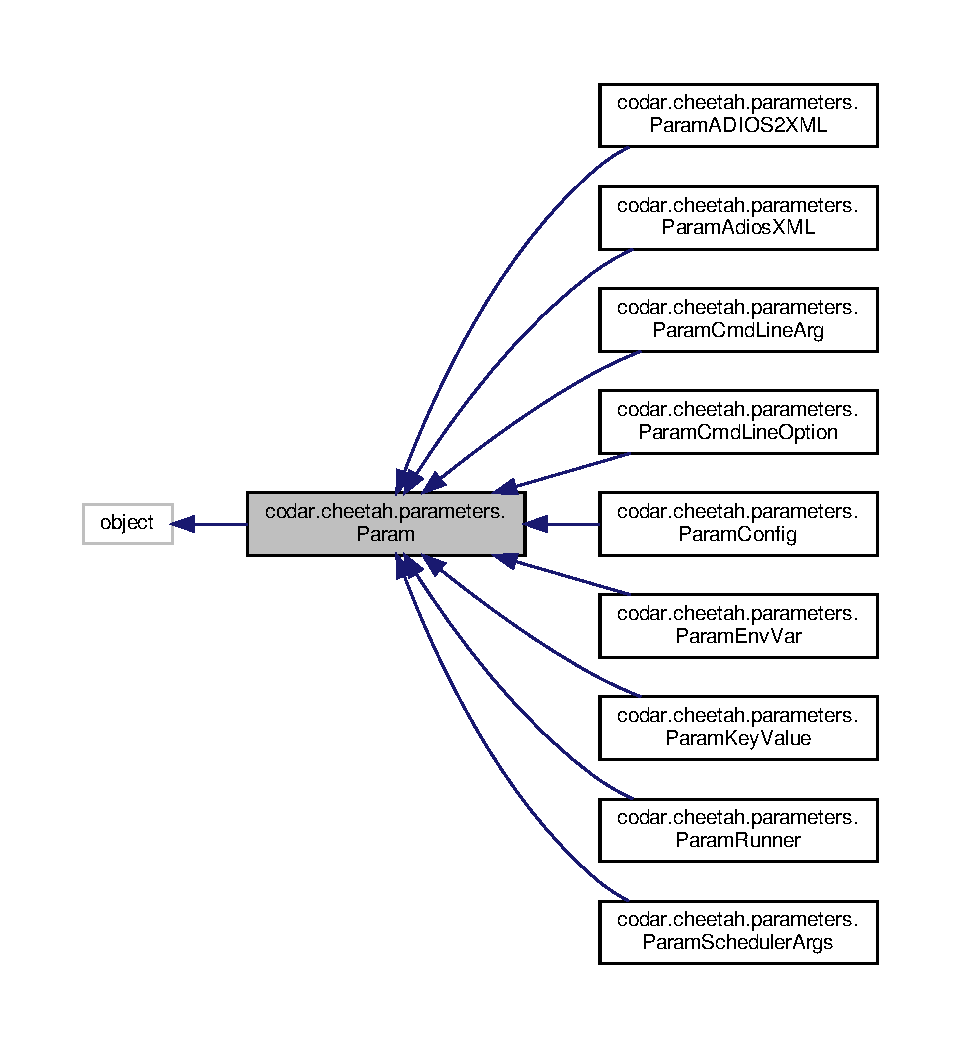
\includegraphics[width=350pt]{classcodar_1_1cheetah_1_1parameters_1_1_param__inherit__graph}
\end{center}
\end{figure}


Collaboration diagram for codar.\+cheetah.\+parameters.\+Param\+:
\nopagebreak
\begin{figure}[H]
\begin{center}
\leavevmode
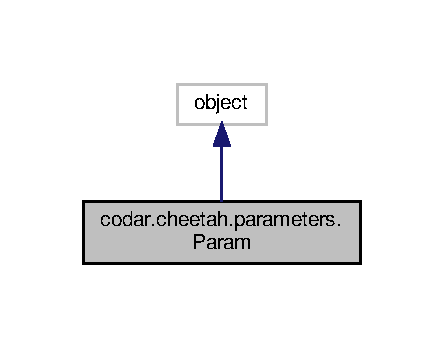
\includegraphics[width=213pt]{classcodar_1_1cheetah_1_1parameters_1_1_param__coll__graph}
\end{center}
\end{figure}
\subsection*{Public Member Functions}
\begin{DoxyCompactItemize}
\item 
def \hyperlink{classcodar_1_1cheetah_1_1parameters_1_1_param_a4c91917ddd306f143286037d02b78034}{\+\_\+\+\_\+init\+\_\+\+\_\+} (self, \hyperlink{classcodar_1_1cheetah_1_1parameters_1_1_param_a5603d43a20cfc6447c3718406ce0669e}{target}, \hyperlink{classcodar_1_1cheetah_1_1parameters_1_1_param_ac9982d62cd18a368a3fbc26541e14209}{name}, \hyperlink{classcodar_1_1cheetah_1_1parameters_1_1_param_aefcc82658f511bddd6605e6ac6e74fbf}{values})
\item 
def \hyperlink{classcodar_1_1cheetah_1_1parameters_1_1_param_ae946fbe90ee7212325e58c9c609b9f60}{\+\_\+\+\_\+get\+\_\+\+\_\+} (self, idx)
\item 
def \hyperlink{classcodar_1_1cheetah_1_1parameters_1_1_param_afe606f18a69519800e93596c1532af8d}{\+\_\+\+\_\+len\+\_\+\+\_\+} (self)
\end{DoxyCompactItemize}
\subsection*{Public Attributes}
\begin{DoxyCompactItemize}
\item 
\hyperlink{classcodar_1_1cheetah_1_1parameters_1_1_param_a5603d43a20cfc6447c3718406ce0669e}{target}
\item 
\hyperlink{classcodar_1_1cheetah_1_1parameters_1_1_param_ac9982d62cd18a368a3fbc26541e14209}{name}
\item 
\hyperlink{classcodar_1_1cheetah_1_1parameters_1_1_param_aefcc82658f511bddd6605e6ac6e74fbf}{values}
\end{DoxyCompactItemize}


\subsection{Detailed Description}
\begin{DoxyVerb}Abstract base class representing a parameter to an application. This
includes any method for modifying the run characteristics of an
application - command line, config file, environment variables, different
executable built with diffrent compiler flags.

Every parameter must have a unique name, and must target a specific
application or middleware, e.g. pbs, aprun, or one of the science
codes that make up an application.

Note that if a science application has only one code, it will likely still
involve middlewhere targets like PBS. Using a different target is one way
to model those.

TODO: is it useful to separate the definition of a param and it's values?

TODO: should we require that the name be unique across all targets, or
just within each target? Global uniqueness allows for a simple list of
dict representation of instances, but two level nested dicts may be
more powerful (first level is target, second level is params).\end{DoxyVerb}
 

Definition at line 299 of file parameters.\+py.



\subsection{Constructor \& Destructor Documentation}
\mbox{\Hypertarget{classcodar_1_1cheetah_1_1parameters_1_1_param_a4c91917ddd306f143286037d02b78034}\label{classcodar_1_1cheetah_1_1parameters_1_1_param_a4c91917ddd306f143286037d02b78034}} 
\index{codar\+::cheetah\+::parameters\+::\+Param@{codar\+::cheetah\+::parameters\+::\+Param}!\+\_\+\+\_\+init\+\_\+\+\_\+@{\+\_\+\+\_\+init\+\_\+\+\_\+}}
\index{\+\_\+\+\_\+init\+\_\+\+\_\+@{\+\_\+\+\_\+init\+\_\+\+\_\+}!codar\+::cheetah\+::parameters\+::\+Param@{codar\+::cheetah\+::parameters\+::\+Param}}
\subsubsection{\texorpdfstring{\+\_\+\+\_\+init\+\_\+\+\_\+()}{\_\_init\_\_()}}
{\footnotesize\ttfamily def codar.\+cheetah.\+parameters.\+Param.\+\_\+\+\_\+init\+\_\+\+\_\+ (\begin{DoxyParamCaption}\item[{}]{self,  }\item[{}]{target,  }\item[{}]{name,  }\item[{}]{values }\end{DoxyParamCaption})}



Definition at line 320 of file parameters.\+py.



\subsection{Member Function Documentation}
\mbox{\Hypertarget{classcodar_1_1cheetah_1_1parameters_1_1_param_ae946fbe90ee7212325e58c9c609b9f60}\label{classcodar_1_1cheetah_1_1parameters_1_1_param_ae946fbe90ee7212325e58c9c609b9f60}} 
\index{codar\+::cheetah\+::parameters\+::\+Param@{codar\+::cheetah\+::parameters\+::\+Param}!\+\_\+\+\_\+get\+\_\+\+\_\+@{\+\_\+\+\_\+get\+\_\+\+\_\+}}
\index{\+\_\+\+\_\+get\+\_\+\+\_\+@{\+\_\+\+\_\+get\+\_\+\+\_\+}!codar\+::cheetah\+::parameters\+::\+Param@{codar\+::cheetah\+::parameters\+::\+Param}}
\subsubsection{\texorpdfstring{\+\_\+\+\_\+get\+\_\+\+\_\+()}{\_\_get\_\_()}}
{\footnotesize\ttfamily def codar.\+cheetah.\+parameters.\+Param.\+\_\+\+\_\+get\+\_\+\+\_\+ (\begin{DoxyParamCaption}\item[{}]{self,  }\item[{}]{idx }\end{DoxyParamCaption})}



Definition at line 334 of file parameters.\+py.

\mbox{\Hypertarget{classcodar_1_1cheetah_1_1parameters_1_1_param_afe606f18a69519800e93596c1532af8d}\label{classcodar_1_1cheetah_1_1parameters_1_1_param_afe606f18a69519800e93596c1532af8d}} 
\index{codar\+::cheetah\+::parameters\+::\+Param@{codar\+::cheetah\+::parameters\+::\+Param}!\+\_\+\+\_\+len\+\_\+\+\_\+@{\+\_\+\+\_\+len\+\_\+\+\_\+}}
\index{\+\_\+\+\_\+len\+\_\+\+\_\+@{\+\_\+\+\_\+len\+\_\+\+\_\+}!codar\+::cheetah\+::parameters\+::\+Param@{codar\+::cheetah\+::parameters\+::\+Param}}
\subsubsection{\texorpdfstring{\+\_\+\+\_\+len\+\_\+\+\_\+()}{\_\_len\_\_()}}
{\footnotesize\ttfamily def codar.\+cheetah.\+parameters.\+Param.\+\_\+\+\_\+len\+\_\+\+\_\+ (\begin{DoxyParamCaption}\item[{}]{self }\end{DoxyParamCaption})}



Definition at line 337 of file parameters.\+py.



\subsection{Member Data Documentation}
\mbox{\Hypertarget{classcodar_1_1cheetah_1_1parameters_1_1_param_ac9982d62cd18a368a3fbc26541e14209}\label{classcodar_1_1cheetah_1_1parameters_1_1_param_ac9982d62cd18a368a3fbc26541e14209}} 
\index{codar\+::cheetah\+::parameters\+::\+Param@{codar\+::cheetah\+::parameters\+::\+Param}!name@{name}}
\index{name@{name}!codar\+::cheetah\+::parameters\+::\+Param@{codar\+::cheetah\+::parameters\+::\+Param}}
\subsubsection{\texorpdfstring{name}{name}}
{\footnotesize\ttfamily codar.\+cheetah.\+parameters.\+Param.\+name}



Definition at line 322 of file parameters.\+py.

\mbox{\Hypertarget{classcodar_1_1cheetah_1_1parameters_1_1_param_a5603d43a20cfc6447c3718406ce0669e}\label{classcodar_1_1cheetah_1_1parameters_1_1_param_a5603d43a20cfc6447c3718406ce0669e}} 
\index{codar\+::cheetah\+::parameters\+::\+Param@{codar\+::cheetah\+::parameters\+::\+Param}!target@{target}}
\index{target@{target}!codar\+::cheetah\+::parameters\+::\+Param@{codar\+::cheetah\+::parameters\+::\+Param}}
\subsubsection{\texorpdfstring{target}{target}}
{\footnotesize\ttfamily codar.\+cheetah.\+parameters.\+Param.\+target}



Definition at line 321 of file parameters.\+py.

\mbox{\Hypertarget{classcodar_1_1cheetah_1_1parameters_1_1_param_aefcc82658f511bddd6605e6ac6e74fbf}\label{classcodar_1_1cheetah_1_1parameters_1_1_param_aefcc82658f511bddd6605e6ac6e74fbf}} 
\index{codar\+::cheetah\+::parameters\+::\+Param@{codar\+::cheetah\+::parameters\+::\+Param}!values@{values}}
\index{values@{values}!codar\+::cheetah\+::parameters\+::\+Param@{codar\+::cheetah\+::parameters\+::\+Param}}
\subsubsection{\texorpdfstring{values}{values}}
{\footnotesize\ttfamily codar.\+cheetah.\+parameters.\+Param.\+values}



Definition at line 331 of file parameters.\+py.



The documentation for this class was generated from the following file\+:\begin{DoxyCompactItemize}
\item 
cheetah/\hyperlink{parameters_8py}{parameters.\+py}\end{DoxyCompactItemize}

\hypertarget{classcodar_1_1cheetah_1_1parameters_1_1_param_a_d_i_o_s2_x_m_l}{}\section{codar.\+cheetah.\+parameters.\+Param\+A\+D\+I\+O\+S2\+X\+ML Class Reference}
\label{classcodar_1_1cheetah_1_1parameters_1_1_param_a_d_i_o_s2_x_m_l}\index{codar.\+cheetah.\+parameters.\+Param\+A\+D\+I\+O\+S2\+X\+ML@{codar.\+cheetah.\+parameters.\+Param\+A\+D\+I\+O\+S2\+X\+ML}}


Inheritance diagram for codar.\+cheetah.\+parameters.\+Param\+A\+D\+I\+O\+S2\+X\+ML\+:
\nopagebreak
\begin{figure}[H]
\begin{center}
\leavevmode
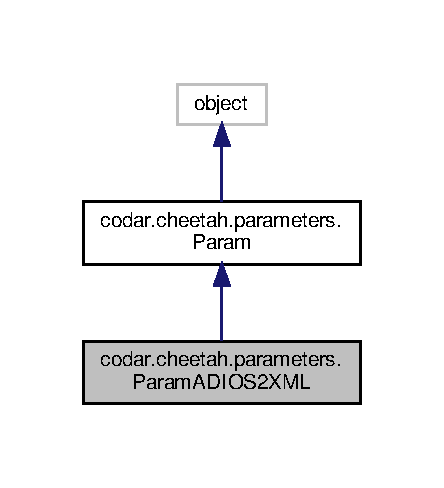
\includegraphics[width=213pt]{classcodar_1_1cheetah_1_1parameters_1_1_param_a_d_i_o_s2_x_m_l__inherit__graph}
\end{center}
\end{figure}


Collaboration diagram for codar.\+cheetah.\+parameters.\+Param\+A\+D\+I\+O\+S2\+X\+ML\+:
\nopagebreak
\begin{figure}[H]
\begin{center}
\leavevmode
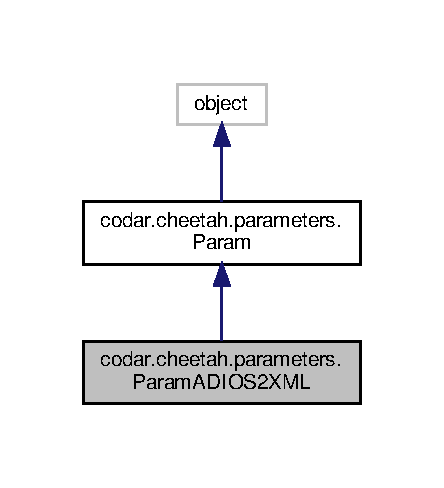
\includegraphics[width=213pt]{classcodar_1_1cheetah_1_1parameters_1_1_param_a_d_i_o_s2_x_m_l__coll__graph}
\end{center}
\end{figure}
\subsection*{Public Member Functions}
\begin{DoxyCompactItemize}
\item 
def \hyperlink{classcodar_1_1cheetah_1_1parameters_1_1_param_a_d_i_o_s2_x_m_l_af754fa92a1b477dc6fedce88a9375d53}{\+\_\+\+\_\+init\+\_\+\+\_\+} (self, \hyperlink{classcodar_1_1cheetah_1_1parameters_1_1_param_a_d_i_o_s2_x_m_l_a81924cb9239a749e787cf68de5dbe508}{rc}, \hyperlink{classcodar_1_1cheetah_1_1parameters_1_1_param_a_d_i_o_s2_x_m_l_a383f4e23cc27b608e08ccab3dcc9163d}{io\+\_\+name}, \hyperlink{classcodar_1_1cheetah_1_1parameters_1_1_param_a_d_i_o_s2_x_m_l_af23a158cb70680fa31d789cf1e1210b1}{operation\+\_\+name}, \hyperlink{classcodar_1_1cheetah_1_1parameters_1_1_param_a_d_i_o_s2_x_m_l_a031e1eec0b1e5d8e6415157b0026ceea}{values})
\end{DoxyCompactItemize}
\subsection*{Public Attributes}
\begin{DoxyCompactItemize}
\item 
\hyperlink{classcodar_1_1cheetah_1_1parameters_1_1_param_a_d_i_o_s2_x_m_l_a81924cb9239a749e787cf68de5dbe508}{rc}
\item 
\hyperlink{classcodar_1_1cheetah_1_1parameters_1_1_param_a_d_i_o_s2_x_m_l_a383f4e23cc27b608e08ccab3dcc9163d}{io\+\_\+name}
\item 
\hyperlink{classcodar_1_1cheetah_1_1parameters_1_1_param_a_d_i_o_s2_x_m_l_af23a158cb70680fa31d789cf1e1210b1}{operation\+\_\+name}
\item 
\hyperlink{classcodar_1_1cheetah_1_1parameters_1_1_param_a_d_i_o_s2_x_m_l_a031e1eec0b1e5d8e6415157b0026ceea}{values}
\end{DoxyCompactItemize}


\subsection{Detailed Description}
\begin{DoxyVerb}Class to represent ADIOS2 XML file parameter options
\end{DoxyVerb}
 

Definition at line 376 of file parameters.\+py.



\subsection{Constructor \& Destructor Documentation}
\mbox{\Hypertarget{classcodar_1_1cheetah_1_1parameters_1_1_param_a_d_i_o_s2_x_m_l_af754fa92a1b477dc6fedce88a9375d53}\label{classcodar_1_1cheetah_1_1parameters_1_1_param_a_d_i_o_s2_x_m_l_af754fa92a1b477dc6fedce88a9375d53}} 
\index{codar\+::cheetah\+::parameters\+::\+Param\+A\+D\+I\+O\+S2\+X\+ML@{codar\+::cheetah\+::parameters\+::\+Param\+A\+D\+I\+O\+S2\+X\+ML}!\+\_\+\+\_\+init\+\_\+\+\_\+@{\+\_\+\+\_\+init\+\_\+\+\_\+}}
\index{\+\_\+\+\_\+init\+\_\+\+\_\+@{\+\_\+\+\_\+init\+\_\+\+\_\+}!codar\+::cheetah\+::parameters\+::\+Param\+A\+D\+I\+O\+S2\+X\+ML@{codar\+::cheetah\+::parameters\+::\+Param\+A\+D\+I\+O\+S2\+X\+ML}}
\subsubsection{\texorpdfstring{\+\_\+\+\_\+init\+\_\+\+\_\+()}{\_\_init\_\_()}}
{\footnotesize\ttfamily def codar.\+cheetah.\+parameters.\+Param\+A\+D\+I\+O\+S2\+X\+M\+L.\+\_\+\+\_\+init\+\_\+\+\_\+ (\begin{DoxyParamCaption}\item[{}]{self,  }\item[{}]{rc,  }\item[{}]{io\+\_\+name,  }\item[{}]{operation\+\_\+name,  }\item[{}]{values }\end{DoxyParamCaption})}

\begin{DoxyVerb}:param rc: name of the run component
:param io_name: name of the io object in the xml file
:param operation_name: engine/transport/var_operation
:param values: a list of dicts of the type
[ { engine_name: {parameters} },
  { engine_name: {parameters} },
  { var_name: {operation_name: {parameters}}}
]
Examples:
[ {"BPFile": {'Threads':1}},
  {"BPFile": {"ProfileUnits": "Microseconds"}}
]
[ { “T”: { “zfp”: {“rate”:18, “accuracy”: 0.01} } },
  { “T”: { “zfp”: {“rate”:18, “accuracy”: 0.001} } },
  { “T”: { “zfp”: {“rate”:18, “accuracy”: 0.0001} } },
  { “T”: { “sz”:  {“rate”:18, “accuracy”: 0.01} } },
]
\end{DoxyVerb}
 

Definition at line 380 of file parameters.\+py.



\subsection{Member Data Documentation}
\mbox{\Hypertarget{classcodar_1_1cheetah_1_1parameters_1_1_param_a_d_i_o_s2_x_m_l_a383f4e23cc27b608e08ccab3dcc9163d}\label{classcodar_1_1cheetah_1_1parameters_1_1_param_a_d_i_o_s2_x_m_l_a383f4e23cc27b608e08ccab3dcc9163d}} 
\index{codar\+::cheetah\+::parameters\+::\+Param\+A\+D\+I\+O\+S2\+X\+ML@{codar\+::cheetah\+::parameters\+::\+Param\+A\+D\+I\+O\+S2\+X\+ML}!io\+\_\+name@{io\+\_\+name}}
\index{io\+\_\+name@{io\+\_\+name}!codar\+::cheetah\+::parameters\+::\+Param\+A\+D\+I\+O\+S2\+X\+ML@{codar\+::cheetah\+::parameters\+::\+Param\+A\+D\+I\+O\+S2\+X\+ML}}
\subsubsection{\texorpdfstring{io\+\_\+name}{io\_name}}
{\footnotesize\ttfamily codar.\+cheetah.\+parameters.\+Param\+A\+D\+I\+O\+S2\+X\+M\+L.\+io\+\_\+name}



Definition at line 404 of file parameters.\+py.

\mbox{\Hypertarget{classcodar_1_1cheetah_1_1parameters_1_1_param_a_d_i_o_s2_x_m_l_af23a158cb70680fa31d789cf1e1210b1}\label{classcodar_1_1cheetah_1_1parameters_1_1_param_a_d_i_o_s2_x_m_l_af23a158cb70680fa31d789cf1e1210b1}} 
\index{codar\+::cheetah\+::parameters\+::\+Param\+A\+D\+I\+O\+S2\+X\+ML@{codar\+::cheetah\+::parameters\+::\+Param\+A\+D\+I\+O\+S2\+X\+ML}!operation\+\_\+name@{operation\+\_\+name}}
\index{operation\+\_\+name@{operation\+\_\+name}!codar\+::cheetah\+::parameters\+::\+Param\+A\+D\+I\+O\+S2\+X\+ML@{codar\+::cheetah\+::parameters\+::\+Param\+A\+D\+I\+O\+S2\+X\+ML}}
\subsubsection{\texorpdfstring{operation\+\_\+name}{operation\_name}}
{\footnotesize\ttfamily codar.\+cheetah.\+parameters.\+Param\+A\+D\+I\+O\+S2\+X\+M\+L.\+operation\+\_\+name}



Definition at line 405 of file parameters.\+py.

\mbox{\Hypertarget{classcodar_1_1cheetah_1_1parameters_1_1_param_a_d_i_o_s2_x_m_l_a81924cb9239a749e787cf68de5dbe508}\label{classcodar_1_1cheetah_1_1parameters_1_1_param_a_d_i_o_s2_x_m_l_a81924cb9239a749e787cf68de5dbe508}} 
\index{codar\+::cheetah\+::parameters\+::\+Param\+A\+D\+I\+O\+S2\+X\+ML@{codar\+::cheetah\+::parameters\+::\+Param\+A\+D\+I\+O\+S2\+X\+ML}!rc@{rc}}
\index{rc@{rc}!codar\+::cheetah\+::parameters\+::\+Param\+A\+D\+I\+O\+S2\+X\+ML@{codar\+::cheetah\+::parameters\+::\+Param\+A\+D\+I\+O\+S2\+X\+ML}}
\subsubsection{\texorpdfstring{rc}{rc}}
{\footnotesize\ttfamily codar.\+cheetah.\+parameters.\+Param\+A\+D\+I\+O\+S2\+X\+M\+L.\+rc}



Definition at line 403 of file parameters.\+py.

\mbox{\Hypertarget{classcodar_1_1cheetah_1_1parameters_1_1_param_a_d_i_o_s2_x_m_l_a031e1eec0b1e5d8e6415157b0026ceea}\label{classcodar_1_1cheetah_1_1parameters_1_1_param_a_d_i_o_s2_x_m_l_a031e1eec0b1e5d8e6415157b0026ceea}} 
\index{codar\+::cheetah\+::parameters\+::\+Param\+A\+D\+I\+O\+S2\+X\+ML@{codar\+::cheetah\+::parameters\+::\+Param\+A\+D\+I\+O\+S2\+X\+ML}!values@{values}}
\index{values@{values}!codar\+::cheetah\+::parameters\+::\+Param\+A\+D\+I\+O\+S2\+X\+ML@{codar\+::cheetah\+::parameters\+::\+Param\+A\+D\+I\+O\+S2\+X\+ML}}
\subsubsection{\texorpdfstring{values}{values}}
{\footnotesize\ttfamily codar.\+cheetah.\+parameters.\+Param\+A\+D\+I\+O\+S2\+X\+M\+L.\+values}



Definition at line 406 of file parameters.\+py.



The documentation for this class was generated from the following file\+:\begin{DoxyCompactItemize}
\item 
\hyperlink{parameters_8py}{parameters.\+py}\end{DoxyCompactItemize}

\hypertarget{classcodar_1_1cheetah_1_1parameters_1_1_param_adios_x_m_l}{}\section{codar.\+cheetah.\+parameters.\+Param\+Adios\+X\+ML Class Reference}
\label{classcodar_1_1cheetah_1_1parameters_1_1_param_adios_x_m_l}\index{codar.\+cheetah.\+parameters.\+Param\+Adios\+X\+ML@{codar.\+cheetah.\+parameters.\+Param\+Adios\+X\+ML}}


Inheritance diagram for codar.\+cheetah.\+parameters.\+Param\+Adios\+X\+ML\+:
\nopagebreak
\begin{figure}[H]
\begin{center}
\leavevmode
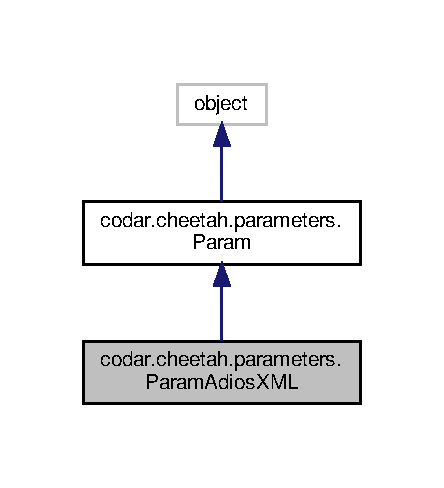
\includegraphics[width=213pt]{classcodar_1_1cheetah_1_1parameters_1_1_param_adios_x_m_l__inherit__graph}
\end{center}
\end{figure}


Collaboration diagram for codar.\+cheetah.\+parameters.\+Param\+Adios\+X\+ML\+:
\nopagebreak
\begin{figure}[H]
\begin{center}
\leavevmode
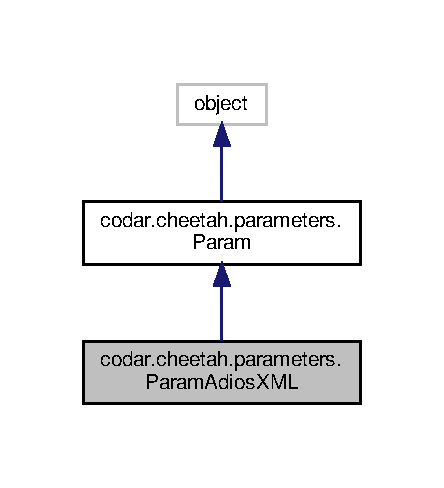
\includegraphics[width=213pt]{classcodar_1_1cheetah_1_1parameters_1_1_param_adios_x_m_l__coll__graph}
\end{center}
\end{figure}
\subsection*{Public Member Functions}
\begin{DoxyCompactItemize}
\item 
def \hyperlink{classcodar_1_1cheetah_1_1parameters_1_1_param_adios_x_m_l_adf9f325576073f42a6e6258403d2632a}{\+\_\+\+\_\+init\+\_\+\+\_\+} (self, \hyperlink{classcodar_1_1cheetah_1_1parameters_1_1_param_a5603d43a20cfc6447c3718406ce0669e}{target}, \hyperlink{classcodar_1_1cheetah_1_1parameters_1_1_param_ac9982d62cd18a368a3fbc26541e14209}{name}, adios\+\_\+xml\+\_\+tags, \hyperlink{classcodar_1_1cheetah_1_1parameters_1_1_param_aefcc82658f511bddd6605e6ac6e74fbf}{values})
\end{DoxyCompactItemize}
\subsection*{Public Attributes}
\begin{DoxyCompactItemize}
\item 
\hyperlink{classcodar_1_1cheetah_1_1parameters_1_1_param_adios_x_m_l_afde8e863f3fb2178723d8f66d6517da2}{param\+\_\+type}
\item 
\hyperlink{classcodar_1_1cheetah_1_1parameters_1_1_param_adios_x_m_l_a248f6d5289be4cad0d6874ece711189b}{group\+\_\+name}
\item 
\hyperlink{classcodar_1_1cheetah_1_1parameters_1_1_param_adios_x_m_l_a8b796c2d1149b202122fcf13a8d31660}{var\+\_\+name}
\end{DoxyCompactItemize}


\subsection{Detailed Description}
\begin{DoxyVerb}Class to represent ADIOS XML Transform.

The transform config is encoded in the name, so transforms on different
variables can be included in the sweep.

Format:
    adios_transform:<group_name>:<var_name>
    adios_transport:<group_name>

Note that the filename is specified in the code definition.
\end{DoxyVerb}
 

Definition at line 349 of file parameters.\+py.



\subsection{Constructor \& Destructor Documentation}
\mbox{\Hypertarget{classcodar_1_1cheetah_1_1parameters_1_1_param_adios_x_m_l_adf9f325576073f42a6e6258403d2632a}\label{classcodar_1_1cheetah_1_1parameters_1_1_param_adios_x_m_l_adf9f325576073f42a6e6258403d2632a}} 
\index{codar\+::cheetah\+::parameters\+::\+Param\+Adios\+X\+ML@{codar\+::cheetah\+::parameters\+::\+Param\+Adios\+X\+ML}!\+\_\+\+\_\+init\+\_\+\+\_\+@{\+\_\+\+\_\+init\+\_\+\+\_\+}}
\index{\+\_\+\+\_\+init\+\_\+\+\_\+@{\+\_\+\+\_\+init\+\_\+\+\_\+}!codar\+::cheetah\+::parameters\+::\+Param\+Adios\+X\+ML@{codar\+::cheetah\+::parameters\+::\+Param\+Adios\+X\+ML}}
\subsubsection{\texorpdfstring{\+\_\+\+\_\+init\+\_\+\+\_\+()}{\_\_init\_\_()}}
{\footnotesize\ttfamily def codar.\+cheetah.\+parameters.\+Param\+Adios\+X\+M\+L.\+\_\+\+\_\+init\+\_\+\+\_\+ (\begin{DoxyParamCaption}\item[{}]{self,  }\item[{}]{target,  }\item[{}]{name,  }\item[{}]{adios\+\_\+xml\+\_\+tags,  }\item[{}]{values }\end{DoxyParamCaption})}



Definition at line 362 of file parameters.\+py.



\subsection{Member Data Documentation}
\mbox{\Hypertarget{classcodar_1_1cheetah_1_1parameters_1_1_param_adios_x_m_l_a248f6d5289be4cad0d6874ece711189b}\label{classcodar_1_1cheetah_1_1parameters_1_1_param_adios_x_m_l_a248f6d5289be4cad0d6874ece711189b}} 
\index{codar\+::cheetah\+::parameters\+::\+Param\+Adios\+X\+ML@{codar\+::cheetah\+::parameters\+::\+Param\+Adios\+X\+ML}!group\+\_\+name@{group\+\_\+name}}
\index{group\+\_\+name@{group\+\_\+name}!codar\+::cheetah\+::parameters\+::\+Param\+Adios\+X\+ML@{codar\+::cheetah\+::parameters\+::\+Param\+Adios\+X\+ML}}
\subsubsection{\texorpdfstring{group\+\_\+name}{group\_name}}
{\footnotesize\ttfamily codar.\+cheetah.\+parameters.\+Param\+Adios\+X\+M\+L.\+group\+\_\+name}



Definition at line 369 of file parameters.\+py.

\mbox{\Hypertarget{classcodar_1_1cheetah_1_1parameters_1_1_param_adios_x_m_l_afde8e863f3fb2178723d8f66d6517da2}\label{classcodar_1_1cheetah_1_1parameters_1_1_param_adios_x_m_l_afde8e863f3fb2178723d8f66d6517da2}} 
\index{codar\+::cheetah\+::parameters\+::\+Param\+Adios\+X\+ML@{codar\+::cheetah\+::parameters\+::\+Param\+Adios\+X\+ML}!param\+\_\+type@{param\+\_\+type}}
\index{param\+\_\+type@{param\+\_\+type}!codar\+::cheetah\+::parameters\+::\+Param\+Adios\+X\+ML@{codar\+::cheetah\+::parameters\+::\+Param\+Adios\+X\+ML}}
\subsubsection{\texorpdfstring{param\+\_\+type}{param\_type}}
{\footnotesize\ttfamily codar.\+cheetah.\+parameters.\+Param\+Adios\+X\+M\+L.\+param\+\_\+type}



Definition at line 368 of file parameters.\+py.

\mbox{\Hypertarget{classcodar_1_1cheetah_1_1parameters_1_1_param_adios_x_m_l_a8b796c2d1149b202122fcf13a8d31660}\label{classcodar_1_1cheetah_1_1parameters_1_1_param_adios_x_m_l_a8b796c2d1149b202122fcf13a8d31660}} 
\index{codar\+::cheetah\+::parameters\+::\+Param\+Adios\+X\+ML@{codar\+::cheetah\+::parameters\+::\+Param\+Adios\+X\+ML}!var\+\_\+name@{var\+\_\+name}}
\index{var\+\_\+name@{var\+\_\+name}!codar\+::cheetah\+::parameters\+::\+Param\+Adios\+X\+ML@{codar\+::cheetah\+::parameters\+::\+Param\+Adios\+X\+ML}}
\subsubsection{\texorpdfstring{var\+\_\+name}{var\_name}}
{\footnotesize\ttfamily codar.\+cheetah.\+parameters.\+Param\+Adios\+X\+M\+L.\+var\+\_\+name}



Definition at line 373 of file parameters.\+py.



The documentation for this class was generated from the following file\+:\begin{DoxyCompactItemize}
\item 
\hyperlink{parameters_8py}{parameters.\+py}\end{DoxyCompactItemize}

\hypertarget{classcodar_1_1cheetah_1_1parameters_1_1_param_cmd_line_arg}{}\section{codar.\+cheetah.\+parameters.\+Param\+Cmd\+Line\+Arg Class Reference}
\label{classcodar_1_1cheetah_1_1parameters_1_1_param_cmd_line_arg}\index{codar.\+cheetah.\+parameters.\+Param\+Cmd\+Line\+Arg@{codar.\+cheetah.\+parameters.\+Param\+Cmd\+Line\+Arg}}


Inheritance diagram for codar.\+cheetah.\+parameters.\+Param\+Cmd\+Line\+Arg\+:
\nopagebreak
\begin{figure}[H]
\begin{center}
\leavevmode
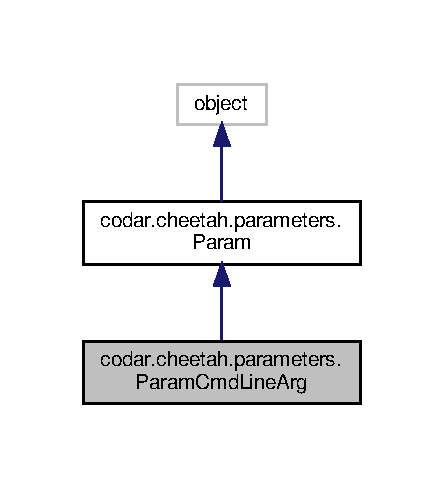
\includegraphics[width=213pt]{classcodar_1_1cheetah_1_1parameters_1_1_param_cmd_line_arg__inherit__graph}
\end{center}
\end{figure}


Collaboration diagram for codar.\+cheetah.\+parameters.\+Param\+Cmd\+Line\+Arg\+:
\nopagebreak
\begin{figure}[H]
\begin{center}
\leavevmode
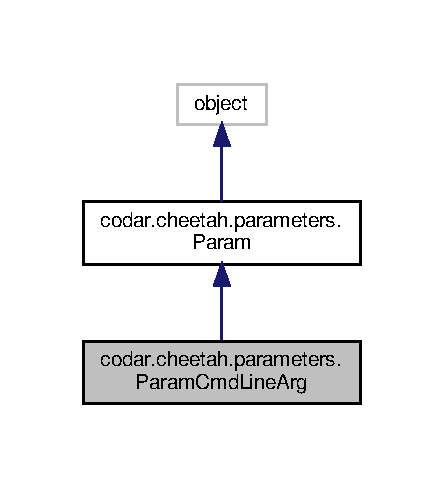
\includegraphics[width=213pt]{classcodar_1_1cheetah_1_1parameters_1_1_param_cmd_line_arg__coll__graph}
\end{center}
\end{figure}
\subsection*{Public Member Functions}
\begin{DoxyCompactItemize}
\item 
def \hyperlink{classcodar_1_1cheetah_1_1parameters_1_1_param_cmd_line_arg_af01175865438c0b3a065aae0790786f1}{\+\_\+\+\_\+init\+\_\+\+\_\+} (self, \hyperlink{classcodar_1_1cheetah_1_1parameters_1_1_param_a5603d43a20cfc6447c3718406ce0669e}{target}, \hyperlink{classcodar_1_1cheetah_1_1parameters_1_1_param_ac9982d62cd18a368a3fbc26541e14209}{name}, \hyperlink{classcodar_1_1cheetah_1_1parameters_1_1_param_cmd_line_arg_a3fc6c85c37895ee7d710475090562ab8}{position}, \hyperlink{classcodar_1_1cheetah_1_1parameters_1_1_param_aefcc82658f511bddd6605e6ac6e74fbf}{values})
\end{DoxyCompactItemize}
\subsection*{Public Attributes}
\begin{DoxyCompactItemize}
\item 
\hyperlink{classcodar_1_1cheetah_1_1parameters_1_1_param_cmd_line_arg_a3fc6c85c37895ee7d710475090562ab8}{position}
\end{DoxyCompactItemize}


\subsection{Detailed Description}
\begin{DoxyVerb}Specification for parameters that are based as a positional command line
argument.\end{DoxyVerb}
 

Definition at line 341 of file parameters.\+py.



\subsection{Constructor \& Destructor Documentation}
\mbox{\Hypertarget{classcodar_1_1cheetah_1_1parameters_1_1_param_cmd_line_arg_af01175865438c0b3a065aae0790786f1}\label{classcodar_1_1cheetah_1_1parameters_1_1_param_cmd_line_arg_af01175865438c0b3a065aae0790786f1}} 
\index{codar\+::cheetah\+::parameters\+::\+Param\+Cmd\+Line\+Arg@{codar\+::cheetah\+::parameters\+::\+Param\+Cmd\+Line\+Arg}!\+\_\+\+\_\+init\+\_\+\+\_\+@{\+\_\+\+\_\+init\+\_\+\+\_\+}}
\index{\+\_\+\+\_\+init\+\_\+\+\_\+@{\+\_\+\+\_\+init\+\_\+\+\_\+}!codar\+::cheetah\+::parameters\+::\+Param\+Cmd\+Line\+Arg@{codar\+::cheetah\+::parameters\+::\+Param\+Cmd\+Line\+Arg}}
\subsubsection{\texorpdfstring{\+\_\+\+\_\+init\+\_\+\+\_\+()}{\_\_init\_\_()}}
{\footnotesize\ttfamily def codar.\+cheetah.\+parameters.\+Param\+Cmd\+Line\+Arg.\+\_\+\+\_\+init\+\_\+\+\_\+ (\begin{DoxyParamCaption}\item[{}]{self,  }\item[{}]{target,  }\item[{}]{name,  }\item[{}]{position,  }\item[{}]{values }\end{DoxyParamCaption})}



Definition at line 344 of file parameters.\+py.



\subsection{Member Data Documentation}
\mbox{\Hypertarget{classcodar_1_1cheetah_1_1parameters_1_1_param_cmd_line_arg_a3fc6c85c37895ee7d710475090562ab8}\label{classcodar_1_1cheetah_1_1parameters_1_1_param_cmd_line_arg_a3fc6c85c37895ee7d710475090562ab8}} 
\index{codar\+::cheetah\+::parameters\+::\+Param\+Cmd\+Line\+Arg@{codar\+::cheetah\+::parameters\+::\+Param\+Cmd\+Line\+Arg}!position@{position}}
\index{position@{position}!codar\+::cheetah\+::parameters\+::\+Param\+Cmd\+Line\+Arg@{codar\+::cheetah\+::parameters\+::\+Param\+Cmd\+Line\+Arg}}
\subsubsection{\texorpdfstring{position}{position}}
{\footnotesize\ttfamily codar.\+cheetah.\+parameters.\+Param\+Cmd\+Line\+Arg.\+position}



Definition at line 346 of file parameters.\+py.



The documentation for this class was generated from the following file\+:\begin{DoxyCompactItemize}
\item 
cheetah/\hyperlink{parameters_8py}{parameters.\+py}\end{DoxyCompactItemize}

\hypertarget{classcodar_1_1cheetah_1_1parameters_1_1_param_cmd_line_option}{}\section{codar.\+cheetah.\+parameters.\+Param\+Cmd\+Line\+Option Class Reference}
\label{classcodar_1_1cheetah_1_1parameters_1_1_param_cmd_line_option}\index{codar.\+cheetah.\+parameters.\+Param\+Cmd\+Line\+Option@{codar.\+cheetah.\+parameters.\+Param\+Cmd\+Line\+Option}}


Inheritance diagram for codar.\+cheetah.\+parameters.\+Param\+Cmd\+Line\+Option\+:
\nopagebreak
\begin{figure}[H]
\begin{center}
\leavevmode
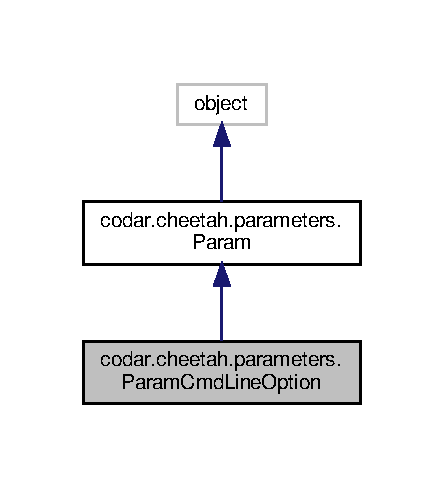
\includegraphics[width=213pt]{classcodar_1_1cheetah_1_1parameters_1_1_param_cmd_line_option__inherit__graph}
\end{center}
\end{figure}


Collaboration diagram for codar.\+cheetah.\+parameters.\+Param\+Cmd\+Line\+Option\+:
\nopagebreak
\begin{figure}[H]
\begin{center}
\leavevmode
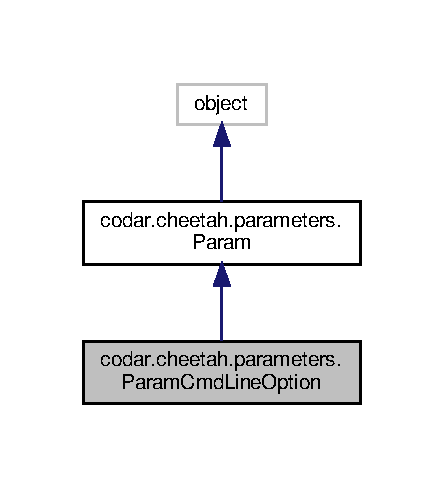
\includegraphics[width=213pt]{classcodar_1_1cheetah_1_1parameters_1_1_param_cmd_line_option__coll__graph}
\end{center}
\end{figure}
\subsection*{Public Member Functions}
\begin{DoxyCompactItemize}
\item 
def \hyperlink{classcodar_1_1cheetah_1_1parameters_1_1_param_cmd_line_option_a7bf4c15694189c9570d3eb3d3b30b7f2}{\+\_\+\+\_\+init\+\_\+\+\_\+} (self, \hyperlink{classcodar_1_1cheetah_1_1parameters_1_1_param_a5603d43a20cfc6447c3718406ce0669e}{target}, \hyperlink{classcodar_1_1cheetah_1_1parameters_1_1_param_ac9982d62cd18a368a3fbc26541e14209}{name}, \hyperlink{classcodar_1_1cheetah_1_1parameters_1_1_param_cmd_line_option_a75dae9b35fe11bc6833cfa0777185e20}{option}, \hyperlink{classcodar_1_1cheetah_1_1parameters_1_1_param_aefcc82658f511bddd6605e6ac6e74fbf}{values})
\end{DoxyCompactItemize}
\subsection*{Public Attributes}
\begin{DoxyCompactItemize}
\item 
\hyperlink{classcodar_1_1cheetah_1_1parameters_1_1_param_cmd_line_option_a75dae9b35fe11bc6833cfa0777185e20}{option}
\end{DoxyCompactItemize}


\subsection{Detailed Description}
\begin{DoxyVerb}Specification for parameters that are based as a labeled command line
option. The option must contain the prefix, e.g. '--output-file' not
'output-file'.\end{DoxyVerb}
 

Definition at line 455 of file parameters.\+py.



\subsection{Constructor \& Destructor Documentation}
\mbox{\Hypertarget{classcodar_1_1cheetah_1_1parameters_1_1_param_cmd_line_option_a7bf4c15694189c9570d3eb3d3b30b7f2}\label{classcodar_1_1cheetah_1_1parameters_1_1_param_cmd_line_option_a7bf4c15694189c9570d3eb3d3b30b7f2}} 
\index{codar\+::cheetah\+::parameters\+::\+Param\+Cmd\+Line\+Option@{codar\+::cheetah\+::parameters\+::\+Param\+Cmd\+Line\+Option}!\+\_\+\+\_\+init\+\_\+\+\_\+@{\+\_\+\+\_\+init\+\_\+\+\_\+}}
\index{\+\_\+\+\_\+init\+\_\+\+\_\+@{\+\_\+\+\_\+init\+\_\+\+\_\+}!codar\+::cheetah\+::parameters\+::\+Param\+Cmd\+Line\+Option@{codar\+::cheetah\+::parameters\+::\+Param\+Cmd\+Line\+Option}}
\subsubsection{\texorpdfstring{\+\_\+\+\_\+init\+\_\+\+\_\+()}{\_\_init\_\_()}}
{\footnotesize\ttfamily def codar.\+cheetah.\+parameters.\+Param\+Cmd\+Line\+Option.\+\_\+\+\_\+init\+\_\+\+\_\+ (\begin{DoxyParamCaption}\item[{}]{self,  }\item[{}]{target,  }\item[{}]{name,  }\item[{}]{option,  }\item[{}]{values }\end{DoxyParamCaption})}



Definition at line 460 of file parameters.\+py.



\subsection{Member Data Documentation}
\mbox{\Hypertarget{classcodar_1_1cheetah_1_1parameters_1_1_param_cmd_line_option_a75dae9b35fe11bc6833cfa0777185e20}\label{classcodar_1_1cheetah_1_1parameters_1_1_param_cmd_line_option_a75dae9b35fe11bc6833cfa0777185e20}} 
\index{codar\+::cheetah\+::parameters\+::\+Param\+Cmd\+Line\+Option@{codar\+::cheetah\+::parameters\+::\+Param\+Cmd\+Line\+Option}!option@{option}}
\index{option@{option}!codar\+::cheetah\+::parameters\+::\+Param\+Cmd\+Line\+Option@{codar\+::cheetah\+::parameters\+::\+Param\+Cmd\+Line\+Option}}
\subsubsection{\texorpdfstring{option}{option}}
{\footnotesize\ttfamily codar.\+cheetah.\+parameters.\+Param\+Cmd\+Line\+Option.\+option}



Definition at line 462 of file parameters.\+py.



The documentation for this class was generated from the following file\+:\begin{DoxyCompactItemize}
\item 
\hyperlink{parameters_8py}{parameters.\+py}\end{DoxyCompactItemize}

\hypertarget{classcodar_1_1cheetah_1_1parameters_1_1_param_config}{}\section{codar.\+cheetah.\+parameters.\+Param\+Config Class Reference}
\label{classcodar_1_1cheetah_1_1parameters_1_1_param_config}\index{codar.\+cheetah.\+parameters.\+Param\+Config@{codar.\+cheetah.\+parameters.\+Param\+Config}}


Inheritance diagram for codar.\+cheetah.\+parameters.\+Param\+Config\+:
\nopagebreak
\begin{figure}[H]
\begin{center}
\leavevmode
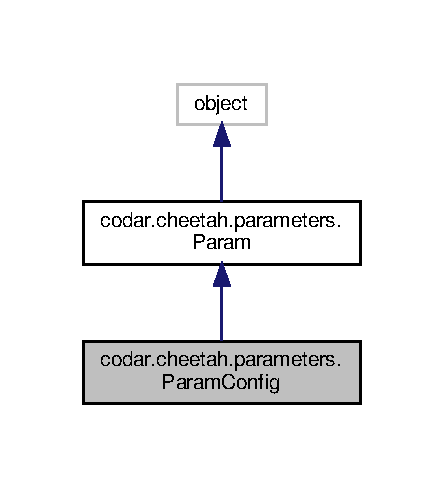
\includegraphics[width=213pt]{classcodar_1_1cheetah_1_1parameters_1_1_param_config__inherit__graph}
\end{center}
\end{figure}


Collaboration diagram for codar.\+cheetah.\+parameters.\+Param\+Config\+:
\nopagebreak
\begin{figure}[H]
\begin{center}
\leavevmode
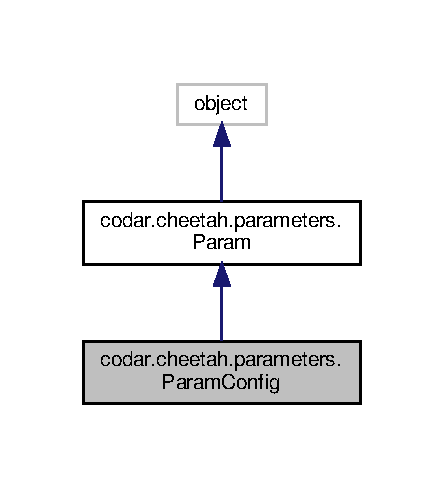
\includegraphics[width=213pt]{classcodar_1_1cheetah_1_1parameters_1_1_param_config__coll__graph}
\end{center}
\end{figure}
\subsection*{Public Member Functions}
\begin{DoxyCompactItemize}
\item 
\mbox{\Hypertarget{classcodar_1_1cheetah_1_1parameters_1_1_param_config_abd78d773a411f8f4ec4b1cddec865644}\label{classcodar_1_1cheetah_1_1parameters_1_1_param_config_abd78d773a411f8f4ec4b1cddec865644}} 
def {\bfseries \+\_\+\+\_\+init\+\_\+\+\_\+} (self, target, name, config\+\_\+filename, match\+\_\+string, values)
\end{DoxyCompactItemize}
\subsection*{Public Attributes}
\begin{DoxyCompactItemize}
\item 
\mbox{\Hypertarget{classcodar_1_1cheetah_1_1parameters_1_1_param_config_a1ea95ac063d51462e652eb8dc4aa22e2}\label{classcodar_1_1cheetah_1_1parameters_1_1_param_config_a1ea95ac063d51462e652eb8dc4aa22e2}} 
{\bfseries config\+\_\+filename}
\item 
\mbox{\Hypertarget{classcodar_1_1cheetah_1_1parameters_1_1_param_config_a00bbc6874525462353e4b2b8d187dcce}\label{classcodar_1_1cheetah_1_1parameters_1_1_param_config_a00bbc6874525462353e4b2b8d187dcce}} 
{\bfseries match\+\_\+string}
\end{DoxyCompactItemize}


\subsection{Detailed Description}
\begin{DoxyVerb}Class to represent a simple literal string replace in a config file.

Note that the filename must be added to the inputs list as well, to be
copied to each run directory.
\end{DoxyVerb}
 

The documentation for this class was generated from the following file\+:\begin{DoxyCompactItemize}
\item 
parameters.\+py\end{DoxyCompactItemize}

\hypertarget{classcodar_1_1cheetah_1_1parameters_1_1_param_env_var}{}\section{codar.\+cheetah.\+parameters.\+Param\+Env\+Var Class Reference}
\label{classcodar_1_1cheetah_1_1parameters_1_1_param_env_var}\index{codar.\+cheetah.\+parameters.\+Param\+Env\+Var@{codar.\+cheetah.\+parameters.\+Param\+Env\+Var}}


Inheritance diagram for codar.\+cheetah.\+parameters.\+Param\+Env\+Var\+:
\nopagebreak
\begin{figure}[H]
\begin{center}
\leavevmode
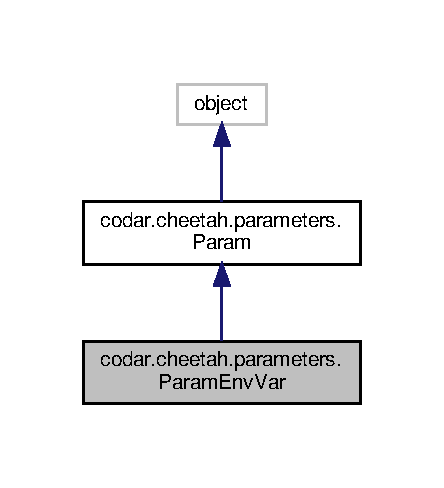
\includegraphics[width=213pt]{classcodar_1_1cheetah_1_1parameters_1_1_param_env_var__inherit__graph}
\end{center}
\end{figure}


Collaboration diagram for codar.\+cheetah.\+parameters.\+Param\+Env\+Var\+:
\nopagebreak
\begin{figure}[H]
\begin{center}
\leavevmode
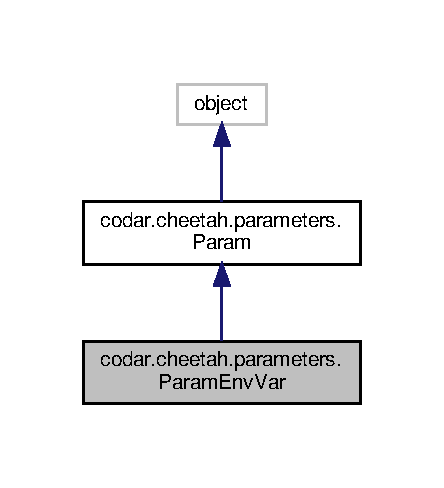
\includegraphics[width=213pt]{classcodar_1_1cheetah_1_1parameters_1_1_param_env_var__coll__graph}
\end{center}
\end{figure}
\subsection*{Public Member Functions}
\begin{DoxyCompactItemize}
\item 
def \hyperlink{classcodar_1_1cheetah_1_1parameters_1_1_param_env_var_a7f0389cec4b151e86fc41fc1548657bd}{\+\_\+\+\_\+init\+\_\+\+\_\+} (self, \hyperlink{classcodar_1_1cheetah_1_1parameters_1_1_param_a5603d43a20cfc6447c3718406ce0669e}{target}, \hyperlink{classcodar_1_1cheetah_1_1parameters_1_1_param_ac9982d62cd18a368a3fbc26541e14209}{name}, \hyperlink{classcodar_1_1cheetah_1_1parameters_1_1_param_env_var_acb91e037a8f36b24a8588b808ad70444}{option}, \hyperlink{classcodar_1_1cheetah_1_1parameters_1_1_param_aefcc82658f511bddd6605e6ac6e74fbf}{values})
\end{DoxyCompactItemize}
\subsection*{Public Attributes}
\begin{DoxyCompactItemize}
\item 
\hyperlink{classcodar_1_1cheetah_1_1parameters_1_1_param_env_var_acb91e037a8f36b24a8588b808ad70444}{option}
\end{DoxyCompactItemize}


\subsection{Detailed Description}


Definition at line 465 of file parameters.\+py.



\subsection{Constructor \& Destructor Documentation}
\mbox{\Hypertarget{classcodar_1_1cheetah_1_1parameters_1_1_param_env_var_a7f0389cec4b151e86fc41fc1548657bd}\label{classcodar_1_1cheetah_1_1parameters_1_1_param_env_var_a7f0389cec4b151e86fc41fc1548657bd}} 
\index{codar\+::cheetah\+::parameters\+::\+Param\+Env\+Var@{codar\+::cheetah\+::parameters\+::\+Param\+Env\+Var}!\+\_\+\+\_\+init\+\_\+\+\_\+@{\+\_\+\+\_\+init\+\_\+\+\_\+}}
\index{\+\_\+\+\_\+init\+\_\+\+\_\+@{\+\_\+\+\_\+init\+\_\+\+\_\+}!codar\+::cheetah\+::parameters\+::\+Param\+Env\+Var@{codar\+::cheetah\+::parameters\+::\+Param\+Env\+Var}}
\subsubsection{\texorpdfstring{\+\_\+\+\_\+init\+\_\+\+\_\+()}{\_\_init\_\_()}}
{\footnotesize\ttfamily def codar.\+cheetah.\+parameters.\+Param\+Env\+Var.\+\_\+\+\_\+init\+\_\+\+\_\+ (\begin{DoxyParamCaption}\item[{}]{self,  }\item[{}]{target,  }\item[{}]{name,  }\item[{}]{option,  }\item[{}]{values }\end{DoxyParamCaption})}



Definition at line 466 of file parameters.\+py.



\subsection{Member Data Documentation}
\mbox{\Hypertarget{classcodar_1_1cheetah_1_1parameters_1_1_param_env_var_acb91e037a8f36b24a8588b808ad70444}\label{classcodar_1_1cheetah_1_1parameters_1_1_param_env_var_acb91e037a8f36b24a8588b808ad70444}} 
\index{codar\+::cheetah\+::parameters\+::\+Param\+Env\+Var@{codar\+::cheetah\+::parameters\+::\+Param\+Env\+Var}!option@{option}}
\index{option@{option}!codar\+::cheetah\+::parameters\+::\+Param\+Env\+Var@{codar\+::cheetah\+::parameters\+::\+Param\+Env\+Var}}
\subsubsection{\texorpdfstring{option}{option}}
{\footnotesize\ttfamily codar.\+cheetah.\+parameters.\+Param\+Env\+Var.\+option}



Definition at line 468 of file parameters.\+py.



The documentation for this class was generated from the following file\+:\begin{DoxyCompactItemize}
\item 
cheetah/\hyperlink{parameters_8py}{parameters.\+py}\end{DoxyCompactItemize}

\hypertarget{classcodar_1_1cheetah_1_1parameters_1_1_parameter_value}{}\section{codar.\+cheetah.\+parameters.\+Parameter\+Value Class Reference}
\label{classcodar_1_1cheetah_1_1parameters_1_1_parameter_value}\index{codar.\+cheetah.\+parameters.\+Parameter\+Value@{codar.\+cheetah.\+parameters.\+Parameter\+Value}}


Inheritance diagram for codar.\+cheetah.\+parameters.\+Parameter\+Value\+:
\nopagebreak
\begin{figure}[H]
\begin{center}
\leavevmode
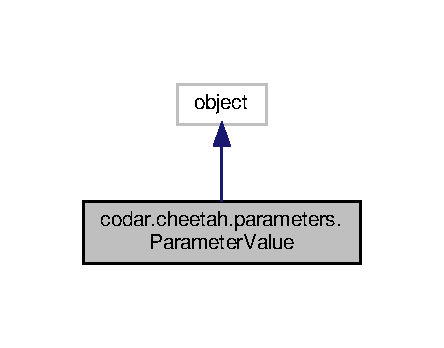
\includegraphics[width=213pt]{classcodar_1_1cheetah_1_1parameters_1_1_parameter_value__inherit__graph}
\end{center}
\end{figure}


Collaboration diagram for codar.\+cheetah.\+parameters.\+Parameter\+Value\+:
\nopagebreak
\begin{figure}[H]
\begin{center}
\leavevmode
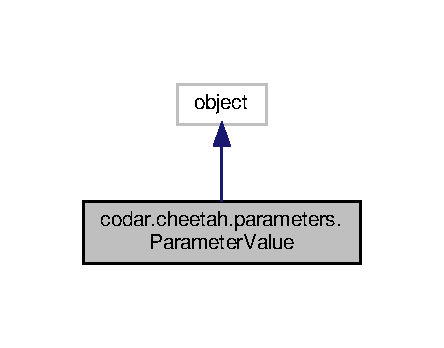
\includegraphics[width=213pt]{classcodar_1_1cheetah_1_1parameters_1_1_parameter_value__coll__graph}
\end{center}
\end{figure}
\subsection*{Public Member Functions}
\begin{DoxyCompactItemize}
\item 
def \hyperlink{classcodar_1_1cheetah_1_1parameters_1_1_parameter_value_ae19c1175ff199c5405518564ec81fa56}{\+\_\+\+\_\+init\+\_\+\+\_\+} (self, parameter, value\+\_\+index)
\item 
def \hyperlink{classcodar_1_1cheetah_1_1parameters_1_1_parameter_value_a984544b6535a16032e725c503f9cba38}{\+\_\+\+\_\+getattr\+\_\+\+\_\+} (self, name)
\item 
def \hyperlink{classcodar_1_1cheetah_1_1parameters_1_1_parameter_value_aad9f920a002859ecec18f5f1ef6085e0}{is\+\_\+type} (self, parameter\+\_\+class)
\end{DoxyCompactItemize}
\subsection*{Public Attributes}
\begin{DoxyCompactItemize}
\item 
\hyperlink{classcodar_1_1cheetah_1_1parameters_1_1_parameter_value_a270382b19fffc9efa6dd17119b8e1ba8}{value}
\end{DoxyCompactItemize}


\subsection{Detailed Description}
\begin{DoxyVerb}Convenience classes for tracking a specific value of a parameter.
Proxies to underlying parameter object, adds a `value` instance
variable.

TODO: this is kind of hacky, is there a better way?
\end{DoxyVerb}
 

Definition at line 80 of file parameters.\+py.



\subsection{Constructor \& Destructor Documentation}
\mbox{\Hypertarget{classcodar_1_1cheetah_1_1parameters_1_1_parameter_value_ae19c1175ff199c5405518564ec81fa56}\label{classcodar_1_1cheetah_1_1parameters_1_1_parameter_value_ae19c1175ff199c5405518564ec81fa56}} 
\index{codar\+::cheetah\+::parameters\+::\+Parameter\+Value@{codar\+::cheetah\+::parameters\+::\+Parameter\+Value}!\+\_\+\+\_\+init\+\_\+\+\_\+@{\+\_\+\+\_\+init\+\_\+\+\_\+}}
\index{\+\_\+\+\_\+init\+\_\+\+\_\+@{\+\_\+\+\_\+init\+\_\+\+\_\+}!codar\+::cheetah\+::parameters\+::\+Parameter\+Value@{codar\+::cheetah\+::parameters\+::\+Parameter\+Value}}
\subsubsection{\texorpdfstring{\+\_\+\+\_\+init\+\_\+\+\_\+()}{\_\_init\_\_()}}
{\footnotesize\ttfamily def codar.\+cheetah.\+parameters.\+Parameter\+Value.\+\_\+\+\_\+init\+\_\+\+\_\+ (\begin{DoxyParamCaption}\item[{}]{self,  }\item[{}]{parameter,  }\item[{}]{value\+\_\+index }\end{DoxyParamCaption})}



Definition at line 88 of file parameters.\+py.



\subsection{Member Function Documentation}
\mbox{\Hypertarget{classcodar_1_1cheetah_1_1parameters_1_1_parameter_value_a984544b6535a16032e725c503f9cba38}\label{classcodar_1_1cheetah_1_1parameters_1_1_parameter_value_a984544b6535a16032e725c503f9cba38}} 
\index{codar\+::cheetah\+::parameters\+::\+Parameter\+Value@{codar\+::cheetah\+::parameters\+::\+Parameter\+Value}!\+\_\+\+\_\+getattr\+\_\+\+\_\+@{\+\_\+\+\_\+getattr\+\_\+\+\_\+}}
\index{\+\_\+\+\_\+getattr\+\_\+\+\_\+@{\+\_\+\+\_\+getattr\+\_\+\+\_\+}!codar\+::cheetah\+::parameters\+::\+Parameter\+Value@{codar\+::cheetah\+::parameters\+::\+Parameter\+Value}}
\subsubsection{\texorpdfstring{\+\_\+\+\_\+getattr\+\_\+\+\_\+()}{\_\_getattr\_\_()}}
{\footnotesize\ttfamily def codar.\+cheetah.\+parameters.\+Parameter\+Value.\+\_\+\+\_\+getattr\+\_\+\+\_\+ (\begin{DoxyParamCaption}\item[{}]{self,  }\item[{}]{name }\end{DoxyParamCaption})}



Definition at line 92 of file parameters.\+py.

\mbox{\Hypertarget{classcodar_1_1cheetah_1_1parameters_1_1_parameter_value_aad9f920a002859ecec18f5f1ef6085e0}\label{classcodar_1_1cheetah_1_1parameters_1_1_parameter_value_aad9f920a002859ecec18f5f1ef6085e0}} 
\index{codar\+::cheetah\+::parameters\+::\+Parameter\+Value@{codar\+::cheetah\+::parameters\+::\+Parameter\+Value}!is\+\_\+type@{is\+\_\+type}}
\index{is\+\_\+type@{is\+\_\+type}!codar\+::cheetah\+::parameters\+::\+Parameter\+Value@{codar\+::cheetah\+::parameters\+::\+Parameter\+Value}}
\subsubsection{\texorpdfstring{is\+\_\+type()}{is\_type()}}
{\footnotesize\ttfamily def codar.\+cheetah.\+parameters.\+Parameter\+Value.\+is\+\_\+type (\begin{DoxyParamCaption}\item[{}]{self,  }\item[{}]{parameter\+\_\+class }\end{DoxyParamCaption})}



Definition at line 97 of file parameters.\+py.



\subsection{Member Data Documentation}
\mbox{\Hypertarget{classcodar_1_1cheetah_1_1parameters_1_1_parameter_value_a270382b19fffc9efa6dd17119b8e1ba8}\label{classcodar_1_1cheetah_1_1parameters_1_1_parameter_value_a270382b19fffc9efa6dd17119b8e1ba8}} 
\index{codar\+::cheetah\+::parameters\+::\+Parameter\+Value@{codar\+::cheetah\+::parameters\+::\+Parameter\+Value}!value@{value}}
\index{value@{value}!codar\+::cheetah\+::parameters\+::\+Parameter\+Value@{codar\+::cheetah\+::parameters\+::\+Parameter\+Value}}
\subsubsection{\texorpdfstring{value}{value}}
{\footnotesize\ttfamily codar.\+cheetah.\+parameters.\+Parameter\+Value.\+value}



Definition at line 90 of file parameters.\+py.



The documentation for this class was generated from the following file\+:\begin{DoxyCompactItemize}
\item 
cheetah/\hyperlink{parameters_8py}{parameters.\+py}\end{DoxyCompactItemize}

\hypertarget{classcodar_1_1cheetah_1_1parameters_1_1_param_key_value}{}\section{codar.\+cheetah.\+parameters.\+Param\+Key\+Value Class Reference}
\label{classcodar_1_1cheetah_1_1parameters_1_1_param_key_value}\index{codar.\+cheetah.\+parameters.\+Param\+Key\+Value@{codar.\+cheetah.\+parameters.\+Param\+Key\+Value}}


Inheritance diagram for codar.\+cheetah.\+parameters.\+Param\+Key\+Value\+:
\nopagebreak
\begin{figure}[H]
\begin{center}
\leavevmode
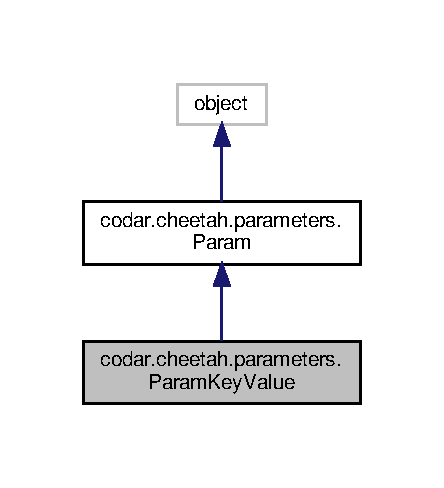
\includegraphics[width=213pt]{classcodar_1_1cheetah_1_1parameters_1_1_param_key_value__inherit__graph}
\end{center}
\end{figure}


Collaboration diagram for codar.\+cheetah.\+parameters.\+Param\+Key\+Value\+:
\nopagebreak
\begin{figure}[H]
\begin{center}
\leavevmode
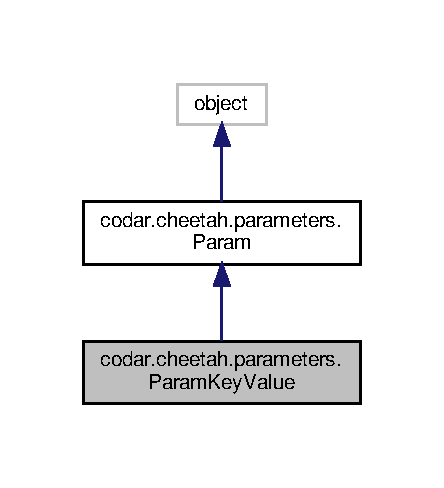
\includegraphics[width=213pt]{classcodar_1_1cheetah_1_1parameters_1_1_param_key_value__coll__graph}
\end{center}
\end{figure}
\subsection*{Public Member Functions}
\begin{DoxyCompactItemize}
\item 
def \hyperlink{classcodar_1_1cheetah_1_1parameters_1_1_param_key_value_acbd81ea2c61adc66c1e5e9f150d9cc39}{\+\_\+\+\_\+init\+\_\+\+\_\+} (self, \hyperlink{classcodar_1_1cheetah_1_1parameters_1_1_param_a5603d43a20cfc6447c3718406ce0669e}{target}, \hyperlink{classcodar_1_1cheetah_1_1parameters_1_1_param_ac9982d62cd18a368a3fbc26541e14209}{name}, \hyperlink{classcodar_1_1cheetah_1_1parameters_1_1_param_key_value_ac463b82e60e626e89e37d267803294ac}{config\+\_\+filename}, \hyperlink{classcodar_1_1cheetah_1_1parameters_1_1_param_key_value_aed81003e4524c70ca0329433fa677f6c}{key\+\_\+name}, \hyperlink{classcodar_1_1cheetah_1_1parameters_1_1_param_aefcc82658f511bddd6605e6ac6e74fbf}{values})
\end{DoxyCompactItemize}
\subsection*{Public Attributes}
\begin{DoxyCompactItemize}
\item 
\hyperlink{classcodar_1_1cheetah_1_1parameters_1_1_param_key_value_ac463b82e60e626e89e37d267803294ac}{config\+\_\+filename}
\item 
\hyperlink{classcodar_1_1cheetah_1_1parameters_1_1_param_key_value_aed81003e4524c70ca0329433fa677f6c}{key\+\_\+name}
\end{DoxyCompactItemize}


\subsection{Detailed Description}
\begin{DoxyVerb}Class to represent replacement of the value in a config file with
'k = v' formatted lines. This should work with various formats, including
fortran namelist and INI, by ignoring lines that don't match the
simple k = v pattern. It has the advantage of being flexible, but the
disadvantage of not understanding sections or other more complicated
structure in config files. Also does not do any quoting - if required,
the spec writer should include literal quotes around the values.

Note that the filename must be added to the inputs list as well, to be
copied to each run directory.
\end{DoxyVerb}
 

Definition at line 436 of file parameters.\+py.



\subsection{Constructor \& Destructor Documentation}
\mbox{\Hypertarget{classcodar_1_1cheetah_1_1parameters_1_1_param_key_value_acbd81ea2c61adc66c1e5e9f150d9cc39}\label{classcodar_1_1cheetah_1_1parameters_1_1_param_key_value_acbd81ea2c61adc66c1e5e9f150d9cc39}} 
\index{codar\+::cheetah\+::parameters\+::\+Param\+Key\+Value@{codar\+::cheetah\+::parameters\+::\+Param\+Key\+Value}!\+\_\+\+\_\+init\+\_\+\+\_\+@{\+\_\+\+\_\+init\+\_\+\+\_\+}}
\index{\+\_\+\+\_\+init\+\_\+\+\_\+@{\+\_\+\+\_\+init\+\_\+\+\_\+}!codar\+::cheetah\+::parameters\+::\+Param\+Key\+Value@{codar\+::cheetah\+::parameters\+::\+Param\+Key\+Value}}
\subsubsection{\texorpdfstring{\+\_\+\+\_\+init\+\_\+\+\_\+()}{\_\_init\_\_()}}
{\footnotesize\ttfamily def codar.\+cheetah.\+parameters.\+Param\+Key\+Value.\+\_\+\+\_\+init\+\_\+\+\_\+ (\begin{DoxyParamCaption}\item[{}]{self,  }\item[{}]{target,  }\item[{}]{name,  }\item[{}]{config\+\_\+filename,  }\item[{}]{key\+\_\+name,  }\item[{}]{values }\end{DoxyParamCaption})}



Definition at line 449 of file parameters.\+py.



\subsection{Member Data Documentation}
\mbox{\Hypertarget{classcodar_1_1cheetah_1_1parameters_1_1_param_key_value_ac463b82e60e626e89e37d267803294ac}\label{classcodar_1_1cheetah_1_1parameters_1_1_param_key_value_ac463b82e60e626e89e37d267803294ac}} 
\index{codar\+::cheetah\+::parameters\+::\+Param\+Key\+Value@{codar\+::cheetah\+::parameters\+::\+Param\+Key\+Value}!config\+\_\+filename@{config\+\_\+filename}}
\index{config\+\_\+filename@{config\+\_\+filename}!codar\+::cheetah\+::parameters\+::\+Param\+Key\+Value@{codar\+::cheetah\+::parameters\+::\+Param\+Key\+Value}}
\subsubsection{\texorpdfstring{config\+\_\+filename}{config\_filename}}
{\footnotesize\ttfamily codar.\+cheetah.\+parameters.\+Param\+Key\+Value.\+config\+\_\+filename}



Definition at line 451 of file parameters.\+py.

\mbox{\Hypertarget{classcodar_1_1cheetah_1_1parameters_1_1_param_key_value_aed81003e4524c70ca0329433fa677f6c}\label{classcodar_1_1cheetah_1_1parameters_1_1_param_key_value_aed81003e4524c70ca0329433fa677f6c}} 
\index{codar\+::cheetah\+::parameters\+::\+Param\+Key\+Value@{codar\+::cheetah\+::parameters\+::\+Param\+Key\+Value}!key\+\_\+name@{key\+\_\+name}}
\index{key\+\_\+name@{key\+\_\+name}!codar\+::cheetah\+::parameters\+::\+Param\+Key\+Value@{codar\+::cheetah\+::parameters\+::\+Param\+Key\+Value}}
\subsubsection{\texorpdfstring{key\+\_\+name}{key\_name}}
{\footnotesize\ttfamily codar.\+cheetah.\+parameters.\+Param\+Key\+Value.\+key\+\_\+name}



Definition at line 452 of file parameters.\+py.



The documentation for this class was generated from the following file\+:\begin{DoxyCompactItemize}
\item 
cheetah/\hyperlink{parameters_8py}{parameters.\+py}\end{DoxyCompactItemize}

\hypertarget{classcodar_1_1cheetah_1_1parameters_1_1_param_runner}{}\section{codar.\+cheetah.\+parameters.\+Param\+Runner Class Reference}
\label{classcodar_1_1cheetah_1_1parameters_1_1_param_runner}\index{codar.\+cheetah.\+parameters.\+Param\+Runner@{codar.\+cheetah.\+parameters.\+Param\+Runner}}


Inheritance diagram for codar.\+cheetah.\+parameters.\+Param\+Runner\+:
\nopagebreak
\begin{figure}[H]
\begin{center}
\leavevmode
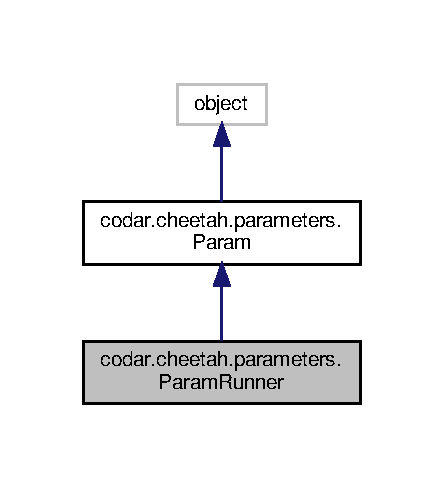
\includegraphics[width=213pt]{classcodar_1_1cheetah_1_1parameters_1_1_param_runner__inherit__graph}
\end{center}
\end{figure}


Collaboration diagram for codar.\+cheetah.\+parameters.\+Param\+Runner\+:
\nopagebreak
\begin{figure}[H]
\begin{center}
\leavevmode
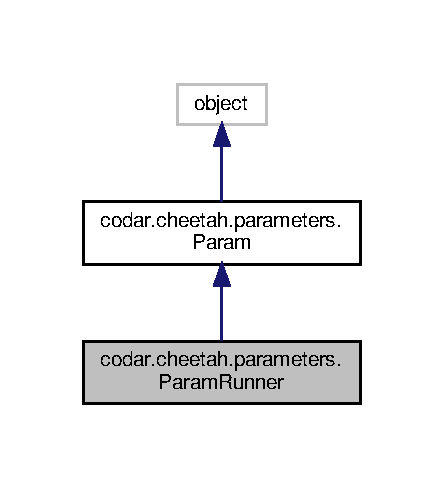
\includegraphics[width=213pt]{classcodar_1_1cheetah_1_1parameters_1_1_param_runner__coll__graph}
\end{center}
\end{figure}
\subsection*{Public Member Functions}
\begin{DoxyCompactItemize}
\item 
def \hyperlink{classcodar_1_1cheetah_1_1parameters_1_1_param_runner_aac032647089038378eedaa25c24775db}{\+\_\+\+\_\+init\+\_\+\+\_\+} (self, \hyperlink{classcodar_1_1cheetah_1_1parameters_1_1_param_a5603d43a20cfc6447c3718406ce0669e}{target}, \hyperlink{classcodar_1_1cheetah_1_1parameters_1_1_param_ac9982d62cd18a368a3fbc26541e14209}{name}, \hyperlink{classcodar_1_1cheetah_1_1parameters_1_1_param_aefcc82658f511bddd6605e6ac6e74fbf}{values})
\end{DoxyCompactItemize}
\subsection*{Additional Inherited Members}


\subsection{Detailed Description}
\begin{DoxyVerb}Specification for parameters that are passed to the runner, e.g.
mpirun, mpilaunch, srun, apirun, but usually still associated with a
specific application code.\end{DoxyVerb}
 

Definition at line 478 of file parameters.\+py.



\subsection{Constructor \& Destructor Documentation}
\mbox{\Hypertarget{classcodar_1_1cheetah_1_1parameters_1_1_param_runner_aac032647089038378eedaa25c24775db}\label{classcodar_1_1cheetah_1_1parameters_1_1_param_runner_aac032647089038378eedaa25c24775db}} 
\index{codar\+::cheetah\+::parameters\+::\+Param\+Runner@{codar\+::cheetah\+::parameters\+::\+Param\+Runner}!\+\_\+\+\_\+init\+\_\+\+\_\+@{\+\_\+\+\_\+init\+\_\+\+\_\+}}
\index{\+\_\+\+\_\+init\+\_\+\+\_\+@{\+\_\+\+\_\+init\+\_\+\+\_\+}!codar\+::cheetah\+::parameters\+::\+Param\+Runner@{codar\+::cheetah\+::parameters\+::\+Param\+Runner}}
\subsubsection{\texorpdfstring{\+\_\+\+\_\+init\+\_\+\+\_\+()}{\_\_init\_\_()}}
{\footnotesize\ttfamily def codar.\+cheetah.\+parameters.\+Param\+Runner.\+\_\+\+\_\+init\+\_\+\+\_\+ (\begin{DoxyParamCaption}\item[{}]{self,  }\item[{}]{target,  }\item[{}]{name,  }\item[{}]{values }\end{DoxyParamCaption})}



Definition at line 482 of file parameters.\+py.



The documentation for this class was generated from the following file\+:\begin{DoxyCompactItemize}
\item 
\hyperlink{parameters_8py}{parameters.\+py}\end{DoxyCompactItemize}

\hypertarget{classcodar_1_1cheetah_1_1parameters_1_1_param_scheduler_args}{}\section{codar.\+cheetah.\+parameters.\+Param\+Scheduler\+Args Class Reference}
\label{classcodar_1_1cheetah_1_1parameters_1_1_param_scheduler_args}\index{codar.\+cheetah.\+parameters.\+Param\+Scheduler\+Args@{codar.\+cheetah.\+parameters.\+Param\+Scheduler\+Args}}


Inheritance diagram for codar.\+cheetah.\+parameters.\+Param\+Scheduler\+Args\+:
\nopagebreak
\begin{figure}[H]
\begin{center}
\leavevmode
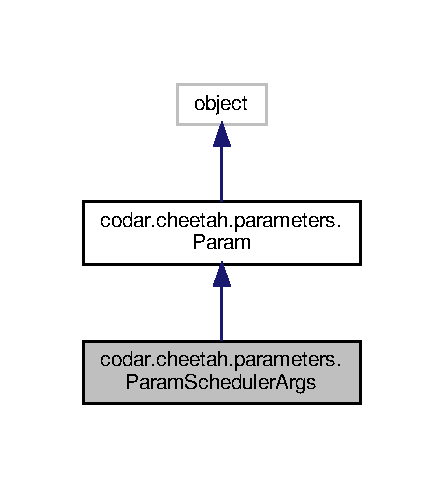
\includegraphics[width=213pt]{classcodar_1_1cheetah_1_1parameters_1_1_param_scheduler_args__inherit__graph}
\end{center}
\end{figure}


Collaboration diagram for codar.\+cheetah.\+parameters.\+Param\+Scheduler\+Args\+:
\nopagebreak
\begin{figure}[H]
\begin{center}
\leavevmode
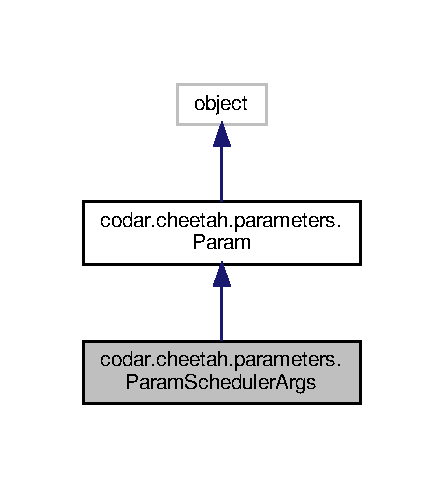
\includegraphics[width=213pt]{classcodar_1_1cheetah_1_1parameters_1_1_param_scheduler_args__coll__graph}
\end{center}
\end{figure}
\subsection*{Public Member Functions}
\begin{DoxyCompactItemize}
\item 
def \hyperlink{classcodar_1_1cheetah_1_1parameters_1_1_param_scheduler_args_abdc6ffa1471d8207fb6de1222791ef87}{\+\_\+\+\_\+init\+\_\+\+\_\+} (self, \hyperlink{classcodar_1_1cheetah_1_1parameters_1_1_param_a5603d43a20cfc6447c3718406ce0669e}{target}, \hyperlink{classcodar_1_1cheetah_1_1parameters_1_1_param_aefcc82658f511bddd6605e6ac6e74fbf}{values})
\end{DoxyCompactItemize}
\subsection*{Additional Inherited Members}


\subsection{Detailed Description}


Definition at line 471 of file parameters.\+py.



\subsection{Constructor \& Destructor Documentation}
\mbox{\Hypertarget{classcodar_1_1cheetah_1_1parameters_1_1_param_scheduler_args_abdc6ffa1471d8207fb6de1222791ef87}\label{classcodar_1_1cheetah_1_1parameters_1_1_param_scheduler_args_abdc6ffa1471d8207fb6de1222791ef87}} 
\index{codar\+::cheetah\+::parameters\+::\+Param\+Scheduler\+Args@{codar\+::cheetah\+::parameters\+::\+Param\+Scheduler\+Args}!\+\_\+\+\_\+init\+\_\+\+\_\+@{\+\_\+\+\_\+init\+\_\+\+\_\+}}
\index{\+\_\+\+\_\+init\+\_\+\+\_\+@{\+\_\+\+\_\+init\+\_\+\+\_\+}!codar\+::cheetah\+::parameters\+::\+Param\+Scheduler\+Args@{codar\+::cheetah\+::parameters\+::\+Param\+Scheduler\+Args}}
\subsubsection{\texorpdfstring{\+\_\+\+\_\+init\+\_\+\+\_\+()}{\_\_init\_\_()}}
{\footnotesize\ttfamily def codar.\+cheetah.\+parameters.\+Param\+Scheduler\+Args.\+\_\+\+\_\+init\+\_\+\+\_\+ (\begin{DoxyParamCaption}\item[{}]{self,  }\item[{}]{target,  }\item[{}]{values }\end{DoxyParamCaption})}



Definition at line 472 of file parameters.\+py.



The documentation for this class was generated from the following file\+:\begin{DoxyCompactItemize}
\item 
cheetah/\hyperlink{parameters_8py}{parameters.\+py}\end{DoxyCompactItemize}

\hypertarget{classcodar_1_1savanna_1_1model_1_1_pipeline}{}\section{codar.\+savanna.\+model.\+Pipeline Class Reference}
\label{classcodar_1_1savanna_1_1model_1_1_pipeline}\index{codar.\+savanna.\+model.\+Pipeline@{codar.\+savanna.\+model.\+Pipeline}}


Inheritance diagram for codar.\+savanna.\+model.\+Pipeline\+:
\nopagebreak
\begin{figure}[H]
\begin{center}
\leavevmode
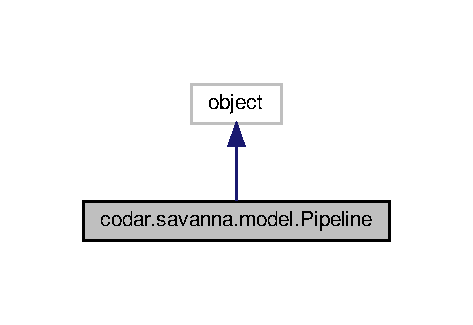
\includegraphics[width=227pt]{classcodar_1_1savanna_1_1model_1_1_pipeline__inherit__graph}
\end{center}
\end{figure}


Collaboration diagram for codar.\+savanna.\+model.\+Pipeline\+:
\nopagebreak
\begin{figure}[H]
\begin{center}
\leavevmode
\includegraphics[width=227pt]{classcodar_1_1savanna_1_1model_1_1_pipeline__coll__graph}
\end{center}
\end{figure}
\subsection*{Public Member Functions}
\begin{DoxyCompactItemize}
\item 
def \hyperlink{classcodar_1_1savanna_1_1model_1_1_pipeline_ada8df2357966f7e3cc7c34d3ee36f9a1}{\+\_\+\+\_\+init\+\_\+\+\_\+} (self, pipe\+\_\+id, \hyperlink{classcodar_1_1savanna_1_1model_1_1_pipeline_aceeec7aae018e27934619f797162d458}{runs}, \hyperlink{classcodar_1_1savanna_1_1model_1_1_pipeline_a2272c691cd2ecb1b11b581341cd5707c}{working\+\_\+dir}, \hyperlink{classcodar_1_1savanna_1_1model_1_1_pipeline_ae5ea9a86523bdbbc9537a37b6d01436c}{total\+\_\+nodes}, \hyperlink{classcodar_1_1savanna_1_1model_1_1_pipeline_a7492ac83160febb20e9a60dad2a9233f}{machine\+\_\+name}, \hyperlink{classcodar_1_1savanna_1_1model_1_1_pipeline_a8f831647499af6eae5696a85abc9a449}{kill\+\_\+on\+\_\+partial\+\_\+failure}=False, \hyperlink{classcodar_1_1savanna_1_1model_1_1_pipeline_a5539114ad7bace8f9753064e3d4a28ec}{post\+\_\+process\+\_\+script}=None, \hyperlink{classcodar_1_1savanna_1_1model_1_1_pipeline_a4568a89046b0fc45c5e6f3f5d80588a1}{post\+\_\+process\+\_\+args}=None, \hyperlink{classcodar_1_1savanna_1_1model_1_1_pipeline_aed4a93e26e62b1878c277a6d9a992fa9}{post\+\_\+process\+\_\+stop\+\_\+on\+\_\+failure}=False, \hyperlink{classcodar_1_1savanna_1_1model_1_1_pipeline_a32c1000ef2bf29a77c0f7ca8849adb64}{node\+\_\+layout}=None, \hyperlink{classcodar_1_1savanna_1_1model_1_1_pipeline_a93c4ea2d9b1714d9f78aba21c1507e95}{launch\+\_\+mode}=None)
\item 
def \hyperlink{classcodar_1_1savanna_1_1model_1_1_pipeline_abf71facf9275710199941f0f79997db2}{from\+\_\+data} (cls, data)
\item 
def \hyperlink{classcodar_1_1savanna_1_1model_1_1_pipeline_ad7ddded563710c1a240b850c56a3fd3c}{start} (self, consumer, \hyperlink{classcodar_1_1savanna_1_1model_1_1_pipeline_ae821850c02f50972fa0edb2284ff9c59}{nodes\+\_\+assigned}, runner=None)
\item 
def \hyperlink{classcodar_1_1savanna_1_1model_1_1_pipeline_a0a7fe2d4e57a5604ae9d997caeee2f87}{run\+\_\+finished} (self, run)
\item 
def \hyperlink{classcodar_1_1savanna_1_1model_1_1_pipeline_a9a21933f3cc3457a161029b4f708997b}{run\+\_\+post\+\_\+process\+\_\+script} (self)
\item 
def \hyperlink{classcodar_1_1savanna_1_1model_1_1_pipeline_a05bcb6afe339fb967d8d358d5c6037ca}{add\+\_\+done\+\_\+callback} (self, fn)
\item 
def \hyperlink{classcodar_1_1savanna_1_1model_1_1_pipeline_aa1656c8b4ec886ef96521dfb137c123b}{remove\+\_\+done\+\_\+callback} (self, fn)
\item 
def \hyperlink{classcodar_1_1savanna_1_1model_1_1_pipeline_ac13dbe4331eff67d4306a11a06199e3e}{add\+\_\+fatal\+\_\+callback} (self, fn)
\item 
def \hyperlink{classcodar_1_1savanna_1_1model_1_1_pipeline_a6ddff7f98a8fd2aa7066343540c8bab0}{remove\+\_\+fatal\+\_\+callback} (self, fn)
\item 
def \hyperlink{classcodar_1_1savanna_1_1model_1_1_pipeline_a0c85356d538d06651c7ed18ceb7c1ce5}{get\+\_\+nodes\+\_\+used} (self)
\item 
def \hyperlink{classcodar_1_1savanna_1_1model_1_1_pipeline_a559b6f3f07dc06fd1c42a33fff9e96f1}{set\+\_\+ppn} (self, ppn)
\item 
def \hyperlink{classcodar_1_1savanna_1_1model_1_1_pipeline_a372fa98a663eccfd0c629e9e92f411f8}{set\+\_\+total\+\_\+nodes} (self)
\item 
def \hyperlink{classcodar_1_1savanna_1_1model_1_1_pipeline_a415914cbdd84133196a9f4c612be5313}{get\+\_\+state} (self)
\item 
def \hyperlink{classcodar_1_1savanna_1_1model_1_1_pipeline_a45f720376f4a44a4d87777c572c7dd3c}{get\+\_\+pids} (self)
\item 
def \hyperlink{classcodar_1_1savanna_1_1model_1_1_pipeline_accc64a044c6e1929d19cbea5718fd0f7}{force\+\_\+kill\+\_\+all} (self)
\item 
def \hyperlink{classcodar_1_1savanna_1_1model_1_1_pipeline_a663e76af6faf61c9791dfc925786a859}{join\+\_\+all} (self)
\end{DoxyCompactItemize}
\subsection*{Public Attributes}
\begin{DoxyCompactItemize}
\item 
\hyperlink{classcodar_1_1savanna_1_1model_1_1_pipeline_ac9d67caac17820b586b007df1411e3f8}{id}
\item 
\hyperlink{classcodar_1_1savanna_1_1model_1_1_pipeline_aceeec7aae018e27934619f797162d458}{runs}
\item 
\hyperlink{classcodar_1_1savanna_1_1model_1_1_pipeline_a2272c691cd2ecb1b11b581341cd5707c}{working\+\_\+dir}
\item 
\hyperlink{classcodar_1_1savanna_1_1model_1_1_pipeline_a8f831647499af6eae5696a85abc9a449}{kill\+\_\+on\+\_\+partial\+\_\+failure}
\item 
\hyperlink{classcodar_1_1savanna_1_1model_1_1_pipeline_a5539114ad7bace8f9753064e3d4a28ec}{post\+\_\+process\+\_\+script}
\item 
\hyperlink{classcodar_1_1savanna_1_1model_1_1_pipeline_a4568a89046b0fc45c5e6f3f5d80588a1}{post\+\_\+process\+\_\+args}
\item 
\hyperlink{classcodar_1_1savanna_1_1model_1_1_pipeline_aed4a93e26e62b1878c277a6d9a992fa9}{post\+\_\+process\+\_\+stop\+\_\+on\+\_\+failure}
\item 
\hyperlink{classcodar_1_1savanna_1_1model_1_1_pipeline_a32c1000ef2bf29a77c0f7ca8849adb64}{node\+\_\+layout}
\item 
\hyperlink{classcodar_1_1savanna_1_1model_1_1_pipeline_a7492ac83160febb20e9a60dad2a9233f}{machine\+\_\+name}
\item 
\hyperlink{classcodar_1_1savanna_1_1model_1_1_pipeline_a10bd363eae4d4b4e00c86fe26c2adedf}{done\+\_\+callbacks}
\item 
\hyperlink{classcodar_1_1savanna_1_1model_1_1_pipeline_a86657c62c6922840292d1f11e455016b}{fatal\+\_\+callbacks}
\item 
\hyperlink{classcodar_1_1savanna_1_1model_1_1_pipeline_a87f9ace8a7b25f52efa9e63821b8ea87}{total\+\_\+procs}
\item 
\hyperlink{classcodar_1_1savanna_1_1model_1_1_pipeline_a461a521150825c07864b23ff66c7cd69}{log\+\_\+prefix}
\item 
\hyperlink{classcodar_1_1savanna_1_1model_1_1_pipeline_ae5ea9a86523bdbbc9537a37b6d01436c}{total\+\_\+nodes}
\item 
\hyperlink{classcodar_1_1savanna_1_1model_1_1_pipeline_a93c4ea2d9b1714d9f78aba21c1507e95}{launch\+\_\+mode}
\item 
\hyperlink{classcodar_1_1savanna_1_1model_1_1_pipeline_ae821850c02f50972fa0edb2284ff9c59}{nodes\+\_\+assigned}
\end{DoxyCompactItemize}


\subsection{Detailed Description}


Definition at line 449 of file model.\+py.



\subsection{Constructor \& Destructor Documentation}
\mbox{\Hypertarget{classcodar_1_1savanna_1_1model_1_1_pipeline_ada8df2357966f7e3cc7c34d3ee36f9a1}\label{classcodar_1_1savanna_1_1model_1_1_pipeline_ada8df2357966f7e3cc7c34d3ee36f9a1}} 
\index{codar\+::savanna\+::model\+::\+Pipeline@{codar\+::savanna\+::model\+::\+Pipeline}!\+\_\+\+\_\+init\+\_\+\+\_\+@{\+\_\+\+\_\+init\+\_\+\+\_\+}}
\index{\+\_\+\+\_\+init\+\_\+\+\_\+@{\+\_\+\+\_\+init\+\_\+\+\_\+}!codar\+::savanna\+::model\+::\+Pipeline@{codar\+::savanna\+::model\+::\+Pipeline}}
\subsubsection{\texorpdfstring{\+\_\+\+\_\+init\+\_\+\+\_\+()}{\_\_init\_\_()}}
{\footnotesize\ttfamily def codar.\+savanna.\+model.\+Pipeline.\+\_\+\+\_\+init\+\_\+\+\_\+ (\begin{DoxyParamCaption}\item[{}]{self,  }\item[{}]{pipe\+\_\+id,  }\item[{}]{runs,  }\item[{}]{working\+\_\+dir,  }\item[{}]{total\+\_\+nodes,  }\item[{}]{machine\+\_\+name,  }\item[{}]{kill\+\_\+on\+\_\+partial\+\_\+failure = {\ttfamily False},  }\item[{}]{post\+\_\+process\+\_\+script = {\ttfamily None},  }\item[{}]{post\+\_\+process\+\_\+args = {\ttfamily None},  }\item[{}]{post\+\_\+process\+\_\+stop\+\_\+on\+\_\+failure = {\ttfamily False},  }\item[{}]{node\+\_\+layout = {\ttfamily None},  }\item[{}]{launch\+\_\+mode = {\ttfamily None} }\end{DoxyParamCaption})}



Definition at line 455 of file model.\+py.



\subsection{Member Function Documentation}
\mbox{\Hypertarget{classcodar_1_1savanna_1_1model_1_1_pipeline_a05bcb6afe339fb967d8d358d5c6037ca}\label{classcodar_1_1savanna_1_1model_1_1_pipeline_a05bcb6afe339fb967d8d358d5c6037ca}} 
\index{codar\+::savanna\+::model\+::\+Pipeline@{codar\+::savanna\+::model\+::\+Pipeline}!add\+\_\+done\+\_\+callback@{add\+\_\+done\+\_\+callback}}
\index{add\+\_\+done\+\_\+callback@{add\+\_\+done\+\_\+callback}!codar\+::savanna\+::model\+::\+Pipeline@{codar\+::savanna\+::model\+::\+Pipeline}}
\subsubsection{\texorpdfstring{add\+\_\+done\+\_\+callback()}{add\_done\_callback()}}
{\footnotesize\ttfamily def codar.\+savanna.\+model.\+Pipeline.\+add\+\_\+done\+\_\+callback (\begin{DoxyParamCaption}\item[{}]{self,  }\item[{}]{fn }\end{DoxyParamCaption})}



Definition at line 818 of file model.\+py.

\mbox{\Hypertarget{classcodar_1_1savanna_1_1model_1_1_pipeline_ac13dbe4331eff67d4306a11a06199e3e}\label{classcodar_1_1savanna_1_1model_1_1_pipeline_ac13dbe4331eff67d4306a11a06199e3e}} 
\index{codar\+::savanna\+::model\+::\+Pipeline@{codar\+::savanna\+::model\+::\+Pipeline}!add\+\_\+fatal\+\_\+callback@{add\+\_\+fatal\+\_\+callback}}
\index{add\+\_\+fatal\+\_\+callback@{add\+\_\+fatal\+\_\+callback}!codar\+::savanna\+::model\+::\+Pipeline@{codar\+::savanna\+::model\+::\+Pipeline}}
\subsubsection{\texorpdfstring{add\+\_\+fatal\+\_\+callback()}{add\_fatal\_callback()}}
{\footnotesize\ttfamily def codar.\+savanna.\+model.\+Pipeline.\+add\+\_\+fatal\+\_\+callback (\begin{DoxyParamCaption}\item[{}]{self,  }\item[{}]{fn }\end{DoxyParamCaption})}



Definition at line 830 of file model.\+py.

\mbox{\Hypertarget{classcodar_1_1savanna_1_1model_1_1_pipeline_accc64a044c6e1929d19cbea5718fd0f7}\label{classcodar_1_1savanna_1_1model_1_1_pipeline_accc64a044c6e1929d19cbea5718fd0f7}} 
\index{codar\+::savanna\+::model\+::\+Pipeline@{codar\+::savanna\+::model\+::\+Pipeline}!force\+\_\+kill\+\_\+all@{force\+\_\+kill\+\_\+all}}
\index{force\+\_\+kill\+\_\+all@{force\+\_\+kill\+\_\+all}!codar\+::savanna\+::model\+::\+Pipeline@{codar\+::savanna\+::model\+::\+Pipeline}}
\subsubsection{\texorpdfstring{force\+\_\+kill\+\_\+all()}{force\_kill\_all()}}
{\footnotesize\ttfamily def codar.\+savanna.\+model.\+Pipeline.\+force\+\_\+kill\+\_\+all (\begin{DoxyParamCaption}\item[{}]{self }\end{DoxyParamCaption})}

\begin{DoxyVerb}Kill all runs and don't run post processing. Note that this call may
block waiting for all runs to be started, to avoid confusing races.
If the pipeline is already done, this does nothing. If one or more
runs are still active, or have not yet been marked as finished, then
it will mark the entire pipeline as killed so it can be re-run from
scratch on a restart if desired.
\end{DoxyVerb}
 

Definition at line 912 of file model.\+py.

\mbox{\Hypertarget{classcodar_1_1savanna_1_1model_1_1_pipeline_abf71facf9275710199941f0f79997db2}\label{classcodar_1_1savanna_1_1model_1_1_pipeline_abf71facf9275710199941f0f79997db2}} 
\index{codar\+::savanna\+::model\+::\+Pipeline@{codar\+::savanna\+::model\+::\+Pipeline}!from\+\_\+data@{from\+\_\+data}}
\index{from\+\_\+data@{from\+\_\+data}!codar\+::savanna\+::model\+::\+Pipeline@{codar\+::savanna\+::model\+::\+Pipeline}}
\subsubsection{\texorpdfstring{from\+\_\+data()}{from\_data()}}
{\footnotesize\ttfamily def codar.\+savanna.\+model.\+Pipeline.\+from\+\_\+data (\begin{DoxyParamCaption}\item[{}]{cls,  }\item[{}]{data }\end{DoxyParamCaption})}

\begin{DoxyVerb}Create Pipeline instance from dictionary data structure, containing
at least "id" and "runs" keys. The "runs" key must have a list of dict,
and each dict is parsed using Run.from_data.
Raises KeyError if a required key is missing.\end{DoxyVerb}
 

Definition at line 497 of file model.\+py.

\mbox{\Hypertarget{classcodar_1_1savanna_1_1model_1_1_pipeline_a0c85356d538d06651c7ed18ceb7c1ce5}\label{classcodar_1_1savanna_1_1model_1_1_pipeline_a0c85356d538d06651c7ed18ceb7c1ce5}} 
\index{codar\+::savanna\+::model\+::\+Pipeline@{codar\+::savanna\+::model\+::\+Pipeline}!get\+\_\+nodes\+\_\+used@{get\+\_\+nodes\+\_\+used}}
\index{get\+\_\+nodes\+\_\+used@{get\+\_\+nodes\+\_\+used}!codar\+::savanna\+::model\+::\+Pipeline@{codar\+::savanna\+::model\+::\+Pipeline}}
\subsubsection{\texorpdfstring{get\+\_\+nodes\+\_\+used()}{get\_nodes\_used()}}
{\footnotesize\ttfamily def codar.\+savanna.\+model.\+Pipeline.\+get\+\_\+nodes\+\_\+used (\begin{DoxyParamCaption}\item[{}]{self }\end{DoxyParamCaption})}



Definition at line 850 of file model.\+py.

\mbox{\Hypertarget{classcodar_1_1savanna_1_1model_1_1_pipeline_a45f720376f4a44a4d87777c572c7dd3c}\label{classcodar_1_1savanna_1_1model_1_1_pipeline_a45f720376f4a44a4d87777c572c7dd3c}} 
\index{codar\+::savanna\+::model\+::\+Pipeline@{codar\+::savanna\+::model\+::\+Pipeline}!get\+\_\+pids@{get\+\_\+pids}}
\index{get\+\_\+pids@{get\+\_\+pids}!codar\+::savanna\+::model\+::\+Pipeline@{codar\+::savanna\+::model\+::\+Pipeline}}
\subsubsection{\texorpdfstring{get\+\_\+pids()}{get\_pids()}}
{\footnotesize\ttfamily def codar.\+savanna.\+model.\+Pipeline.\+get\+\_\+pids (\begin{DoxyParamCaption}\item[{}]{self }\end{DoxyParamCaption})}



Definition at line 908 of file model.\+py.

\mbox{\Hypertarget{classcodar_1_1savanna_1_1model_1_1_pipeline_a415914cbdd84133196a9f4c612be5313}\label{classcodar_1_1savanna_1_1model_1_1_pipeline_a415914cbdd84133196a9f4c612be5313}} 
\index{codar\+::savanna\+::model\+::\+Pipeline@{codar\+::savanna\+::model\+::\+Pipeline}!get\+\_\+state@{get\+\_\+state}}
\index{get\+\_\+state@{get\+\_\+state}!codar\+::savanna\+::model\+::\+Pipeline@{codar\+::savanna\+::model\+::\+Pipeline}}
\subsubsection{\texorpdfstring{get\+\_\+state()}{get\_state()}}
{\footnotesize\ttfamily def codar.\+savanna.\+model.\+Pipeline.\+get\+\_\+state (\begin{DoxyParamCaption}\item[{}]{self }\end{DoxyParamCaption})}



Definition at line 883 of file model.\+py.

\mbox{\Hypertarget{classcodar_1_1savanna_1_1model_1_1_pipeline_a663e76af6faf61c9791dfc925786a859}\label{classcodar_1_1savanna_1_1model_1_1_pipeline_a663e76af6faf61c9791dfc925786a859}} 
\index{codar\+::savanna\+::model\+::\+Pipeline@{codar\+::savanna\+::model\+::\+Pipeline}!join\+\_\+all@{join\+\_\+all}}
\index{join\+\_\+all@{join\+\_\+all}!codar\+::savanna\+::model\+::\+Pipeline@{codar\+::savanna\+::model\+::\+Pipeline}}
\subsubsection{\texorpdfstring{join\+\_\+all()}{join\_all()}}
{\footnotesize\ttfamily def codar.\+savanna.\+model.\+Pipeline.\+join\+\_\+all (\begin{DoxyParamCaption}\item[{}]{self }\end{DoxyParamCaption})}



Definition at line 933 of file model.\+py.

\mbox{\Hypertarget{classcodar_1_1savanna_1_1model_1_1_pipeline_aa1656c8b4ec886ef96521dfb137c123b}\label{classcodar_1_1savanna_1_1model_1_1_pipeline_aa1656c8b4ec886ef96521dfb137c123b}} 
\index{codar\+::savanna\+::model\+::\+Pipeline@{codar\+::savanna\+::model\+::\+Pipeline}!remove\+\_\+done\+\_\+callback@{remove\+\_\+done\+\_\+callback}}
\index{remove\+\_\+done\+\_\+callback@{remove\+\_\+done\+\_\+callback}!codar\+::savanna\+::model\+::\+Pipeline@{codar\+::savanna\+::model\+::\+Pipeline}}
\subsubsection{\texorpdfstring{remove\+\_\+done\+\_\+callback()}{remove\_done\_callback()}}
{\footnotesize\ttfamily def codar.\+savanna.\+model.\+Pipeline.\+remove\+\_\+done\+\_\+callback (\begin{DoxyParamCaption}\item[{}]{self,  }\item[{}]{fn }\end{DoxyParamCaption})}



Definition at line 821 of file model.\+py.

\mbox{\Hypertarget{classcodar_1_1savanna_1_1model_1_1_pipeline_a6ddff7f98a8fd2aa7066343540c8bab0}\label{classcodar_1_1savanna_1_1model_1_1_pipeline_a6ddff7f98a8fd2aa7066343540c8bab0}} 
\index{codar\+::savanna\+::model\+::\+Pipeline@{codar\+::savanna\+::model\+::\+Pipeline}!remove\+\_\+fatal\+\_\+callback@{remove\+\_\+fatal\+\_\+callback}}
\index{remove\+\_\+fatal\+\_\+callback@{remove\+\_\+fatal\+\_\+callback}!codar\+::savanna\+::model\+::\+Pipeline@{codar\+::savanna\+::model\+::\+Pipeline}}
\subsubsection{\texorpdfstring{remove\+\_\+fatal\+\_\+callback()}{remove\_fatal\_callback()}}
{\footnotesize\ttfamily def codar.\+savanna.\+model.\+Pipeline.\+remove\+\_\+fatal\+\_\+callback (\begin{DoxyParamCaption}\item[{}]{self,  }\item[{}]{fn }\end{DoxyParamCaption})}



Definition at line 833 of file model.\+py.

\mbox{\Hypertarget{classcodar_1_1savanna_1_1model_1_1_pipeline_a0a7fe2d4e57a5604ae9d997caeee2f87}\label{classcodar_1_1savanna_1_1model_1_1_pipeline_a0a7fe2d4e57a5604ae9d997caeee2f87}} 
\index{codar\+::savanna\+::model\+::\+Pipeline@{codar\+::savanna\+::model\+::\+Pipeline}!run\+\_\+finished@{run\+\_\+finished}}
\index{run\+\_\+finished@{run\+\_\+finished}!codar\+::savanna\+::model\+::\+Pipeline@{codar\+::savanna\+::model\+::\+Pipeline}}
\subsubsection{\texorpdfstring{run\+\_\+finished()}{run\_finished()}}
{\footnotesize\ttfamily def codar.\+savanna.\+model.\+Pipeline.\+run\+\_\+finished (\begin{DoxyParamCaption}\item[{}]{self,  }\item[{}]{run }\end{DoxyParamCaption})}



Definition at line 744 of file model.\+py.

\mbox{\Hypertarget{classcodar_1_1savanna_1_1model_1_1_pipeline_a9a21933f3cc3457a161029b4f708997b}\label{classcodar_1_1savanna_1_1model_1_1_pipeline_a9a21933f3cc3457a161029b4f708997b}} 
\index{codar\+::savanna\+::model\+::\+Pipeline@{codar\+::savanna\+::model\+::\+Pipeline}!run\+\_\+post\+\_\+process\+\_\+script@{run\+\_\+post\+\_\+process\+\_\+script}}
\index{run\+\_\+post\+\_\+process\+\_\+script@{run\+\_\+post\+\_\+process\+\_\+script}!codar\+::savanna\+::model\+::\+Pipeline@{codar\+::savanna\+::model\+::\+Pipeline}}
\subsubsection{\texorpdfstring{run\+\_\+post\+\_\+process\+\_\+script()}{run\_post\_process\_script()}}
{\footnotesize\ttfamily def codar.\+savanna.\+model.\+Pipeline.\+run\+\_\+post\+\_\+process\+\_\+script (\begin{DoxyParamCaption}\item[{}]{self }\end{DoxyParamCaption})}



Definition at line 772 of file model.\+py.

\mbox{\Hypertarget{classcodar_1_1savanna_1_1model_1_1_pipeline_a559b6f3f07dc06fd1c42a33fff9e96f1}\label{classcodar_1_1savanna_1_1model_1_1_pipeline_a559b6f3f07dc06fd1c42a33fff9e96f1}} 
\index{codar\+::savanna\+::model\+::\+Pipeline@{codar\+::savanna\+::model\+::\+Pipeline}!set\+\_\+ppn@{set\+\_\+ppn}}
\index{set\+\_\+ppn@{set\+\_\+ppn}!codar\+::savanna\+::model\+::\+Pipeline@{codar\+::savanna\+::model\+::\+Pipeline}}
\subsubsection{\texorpdfstring{set\+\_\+ppn()}{set\_ppn()}}
{\footnotesize\ttfamily def codar.\+savanna.\+model.\+Pipeline.\+set\+\_\+ppn (\begin{DoxyParamCaption}\item[{}]{self,  }\item[{}]{ppn }\end{DoxyParamCaption})}

\begin{DoxyVerb}Determine number of nodes needed to run pipeline with the specified
node layout or full occupancy layout with ppn. Also updates runs
to set node and task per node counts.
TODO: This should be set by Cheetah in fobs.json\end{DoxyVerb}
 

Definition at line 855 of file model.\+py.

\mbox{\Hypertarget{classcodar_1_1savanna_1_1model_1_1_pipeline_a372fa98a663eccfd0c629e9e92f411f8}\label{classcodar_1_1savanna_1_1model_1_1_pipeline_a372fa98a663eccfd0c629e9e92f411f8}} 
\index{codar\+::savanna\+::model\+::\+Pipeline@{codar\+::savanna\+::model\+::\+Pipeline}!set\+\_\+total\+\_\+nodes@{set\+\_\+total\+\_\+nodes}}
\index{set\+\_\+total\+\_\+nodes@{set\+\_\+total\+\_\+nodes}!codar\+::savanna\+::model\+::\+Pipeline@{codar\+::savanna\+::model\+::\+Pipeline}}
\subsubsection{\texorpdfstring{set\+\_\+total\+\_\+nodes()}{set\_total\_nodes()}}
{\footnotesize\ttfamily def codar.\+savanna.\+model.\+Pipeline.\+set\+\_\+total\+\_\+nodes (\begin{DoxyParamCaption}\item[{}]{self }\end{DoxyParamCaption})}

\begin{DoxyVerb}To be deprecated
\end{DoxyVerb}
 

Definition at line 877 of file model.\+py.

\mbox{\Hypertarget{classcodar_1_1savanna_1_1model_1_1_pipeline_ad7ddded563710c1a240b850c56a3fd3c}\label{classcodar_1_1savanna_1_1model_1_1_pipeline_ad7ddded563710c1a240b850c56a3fd3c}} 
\index{codar\+::savanna\+::model\+::\+Pipeline@{codar\+::savanna\+::model\+::\+Pipeline}!start@{start}}
\index{start@{start}!codar\+::savanna\+::model\+::\+Pipeline@{codar\+::savanna\+::model\+::\+Pipeline}}
\subsubsection{\texorpdfstring{start()}{start()}}
{\footnotesize\ttfamily def codar.\+savanna.\+model.\+Pipeline.\+start (\begin{DoxyParamCaption}\item[{}]{self,  }\item[{}]{consumer,  }\item[{}]{nodes\+\_\+assigned,  }\item[{}]{runner = {\ttfamily None} }\end{DoxyParamCaption})}



Definition at line 550 of file model.\+py.



\subsection{Member Data Documentation}
\mbox{\Hypertarget{classcodar_1_1savanna_1_1model_1_1_pipeline_a10bd363eae4d4b4e00c86fe26c2adedf}\label{classcodar_1_1savanna_1_1model_1_1_pipeline_a10bd363eae4d4b4e00c86fe26c2adedf}} 
\index{codar\+::savanna\+::model\+::\+Pipeline@{codar\+::savanna\+::model\+::\+Pipeline}!done\+\_\+callbacks@{done\+\_\+callbacks}}
\index{done\+\_\+callbacks@{done\+\_\+callbacks}!codar\+::savanna\+::model\+::\+Pipeline@{codar\+::savanna\+::model\+::\+Pipeline}}
\subsubsection{\texorpdfstring{done\+\_\+callbacks}{done\_callbacks}}
{\footnotesize\ttfamily codar.\+savanna.\+model.\+Pipeline.\+done\+\_\+callbacks}



Definition at line 473 of file model.\+py.

\mbox{\Hypertarget{classcodar_1_1savanna_1_1model_1_1_pipeline_a86657c62c6922840292d1f11e455016b}\label{classcodar_1_1savanna_1_1model_1_1_pipeline_a86657c62c6922840292d1f11e455016b}} 
\index{codar\+::savanna\+::model\+::\+Pipeline@{codar\+::savanna\+::model\+::\+Pipeline}!fatal\+\_\+callbacks@{fatal\+\_\+callbacks}}
\index{fatal\+\_\+callbacks@{fatal\+\_\+callbacks}!codar\+::savanna\+::model\+::\+Pipeline@{codar\+::savanna\+::model\+::\+Pipeline}}
\subsubsection{\texorpdfstring{fatal\+\_\+callbacks}{fatal\_callbacks}}
{\footnotesize\ttfamily codar.\+savanna.\+model.\+Pipeline.\+fatal\+\_\+callbacks}



Definition at line 474 of file model.\+py.

\mbox{\Hypertarget{classcodar_1_1savanna_1_1model_1_1_pipeline_ac9d67caac17820b586b007df1411e3f8}\label{classcodar_1_1savanna_1_1model_1_1_pipeline_ac9d67caac17820b586b007df1411e3f8}} 
\index{codar\+::savanna\+::model\+::\+Pipeline@{codar\+::savanna\+::model\+::\+Pipeline}!id@{id}}
\index{id@{id}!codar\+::savanna\+::model\+::\+Pipeline@{codar\+::savanna\+::model\+::\+Pipeline}}
\subsubsection{\texorpdfstring{id}{id}}
{\footnotesize\ttfamily codar.\+savanna.\+model.\+Pipeline.\+id}



Definition at line 456 of file model.\+py.

\mbox{\Hypertarget{classcodar_1_1savanna_1_1model_1_1_pipeline_a8f831647499af6eae5696a85abc9a449}\label{classcodar_1_1savanna_1_1model_1_1_pipeline_a8f831647499af6eae5696a85abc9a449}} 
\index{codar\+::savanna\+::model\+::\+Pipeline@{codar\+::savanna\+::model\+::\+Pipeline}!kill\+\_\+on\+\_\+partial\+\_\+failure@{kill\+\_\+on\+\_\+partial\+\_\+failure}}
\index{kill\+\_\+on\+\_\+partial\+\_\+failure@{kill\+\_\+on\+\_\+partial\+\_\+failure}!codar\+::savanna\+::model\+::\+Pipeline@{codar\+::savanna\+::model\+::\+Pipeline}}
\subsubsection{\texorpdfstring{kill\+\_\+on\+\_\+partial\+\_\+failure}{kill\_on\_partial\_failure}}
{\footnotesize\ttfamily codar.\+savanna.\+model.\+Pipeline.\+kill\+\_\+on\+\_\+partial\+\_\+failure}



Definition at line 459 of file model.\+py.

\mbox{\Hypertarget{classcodar_1_1savanna_1_1model_1_1_pipeline_a93c4ea2d9b1714d9f78aba21c1507e95}\label{classcodar_1_1savanna_1_1model_1_1_pipeline_a93c4ea2d9b1714d9f78aba21c1507e95}} 
\index{codar\+::savanna\+::model\+::\+Pipeline@{codar\+::savanna\+::model\+::\+Pipeline}!launch\+\_\+mode@{launch\+\_\+mode}}
\index{launch\+\_\+mode@{launch\+\_\+mode}!codar\+::savanna\+::model\+::\+Pipeline@{codar\+::savanna\+::model\+::\+Pipeline}}
\subsubsection{\texorpdfstring{launch\+\_\+mode}{launch\_mode}}
{\footnotesize\ttfamily codar.\+savanna.\+model.\+Pipeline.\+launch\+\_\+mode}



Definition at line 483 of file model.\+py.

\mbox{\Hypertarget{classcodar_1_1savanna_1_1model_1_1_pipeline_a461a521150825c07864b23ff66c7cd69}\label{classcodar_1_1savanna_1_1model_1_1_pipeline_a461a521150825c07864b23ff66c7cd69}} 
\index{codar\+::savanna\+::model\+::\+Pipeline@{codar\+::savanna\+::model\+::\+Pipeline}!log\+\_\+prefix@{log\+\_\+prefix}}
\index{log\+\_\+prefix@{log\+\_\+prefix}!codar\+::savanna\+::model\+::\+Pipeline@{codar\+::savanna\+::model\+::\+Pipeline}}
\subsubsection{\texorpdfstring{log\+\_\+prefix}{log\_prefix}}
{\footnotesize\ttfamily codar.\+savanna.\+model.\+Pipeline.\+log\+\_\+prefix}



Definition at line 476 of file model.\+py.

\mbox{\Hypertarget{classcodar_1_1savanna_1_1model_1_1_pipeline_a7492ac83160febb20e9a60dad2a9233f}\label{classcodar_1_1savanna_1_1model_1_1_pipeline_a7492ac83160febb20e9a60dad2a9233f}} 
\index{codar\+::savanna\+::model\+::\+Pipeline@{codar\+::savanna\+::model\+::\+Pipeline}!machine\+\_\+name@{machine\+\_\+name}}
\index{machine\+\_\+name@{machine\+\_\+name}!codar\+::savanna\+::model\+::\+Pipeline@{codar\+::savanna\+::model\+::\+Pipeline}}
\subsubsection{\texorpdfstring{machine\+\_\+name}{machine\_name}}
{\footnotesize\ttfamily codar.\+savanna.\+model.\+Pipeline.\+machine\+\_\+name}



Definition at line 464 of file model.\+py.

\mbox{\Hypertarget{classcodar_1_1savanna_1_1model_1_1_pipeline_a32c1000ef2bf29a77c0f7ca8849adb64}\label{classcodar_1_1savanna_1_1model_1_1_pipeline_a32c1000ef2bf29a77c0f7ca8849adb64}} 
\index{codar\+::savanna\+::model\+::\+Pipeline@{codar\+::savanna\+::model\+::\+Pipeline}!node\+\_\+layout@{node\+\_\+layout}}
\index{node\+\_\+layout@{node\+\_\+layout}!codar\+::savanna\+::model\+::\+Pipeline@{codar\+::savanna\+::model\+::\+Pipeline}}
\subsubsection{\texorpdfstring{node\+\_\+layout}{node\_layout}}
{\footnotesize\ttfamily codar.\+savanna.\+model.\+Pipeline.\+node\+\_\+layout}



Definition at line 463 of file model.\+py.

\mbox{\Hypertarget{classcodar_1_1savanna_1_1model_1_1_pipeline_ae821850c02f50972fa0edb2284ff9c59}\label{classcodar_1_1savanna_1_1model_1_1_pipeline_ae821850c02f50972fa0edb2284ff9c59}} 
\index{codar\+::savanna\+::model\+::\+Pipeline@{codar\+::savanna\+::model\+::\+Pipeline}!nodes\+\_\+assigned@{nodes\+\_\+assigned}}
\index{nodes\+\_\+assigned@{nodes\+\_\+assigned}!codar\+::savanna\+::model\+::\+Pipeline@{codar\+::savanna\+::model\+::\+Pipeline}}
\subsubsection{\texorpdfstring{nodes\+\_\+assigned}{nodes\_assigned}}
{\footnotesize\ttfamily codar.\+savanna.\+model.\+Pipeline.\+nodes\+\_\+assigned}



Definition at line 487 of file model.\+py.

\mbox{\Hypertarget{classcodar_1_1savanna_1_1model_1_1_pipeline_a4568a89046b0fc45c5e6f3f5d80588a1}\label{classcodar_1_1savanna_1_1model_1_1_pipeline_a4568a89046b0fc45c5e6f3f5d80588a1}} 
\index{codar\+::savanna\+::model\+::\+Pipeline@{codar\+::savanna\+::model\+::\+Pipeline}!post\+\_\+process\+\_\+args@{post\+\_\+process\+\_\+args}}
\index{post\+\_\+process\+\_\+args@{post\+\_\+process\+\_\+args}!codar\+::savanna\+::model\+::\+Pipeline@{codar\+::savanna\+::model\+::\+Pipeline}}
\subsubsection{\texorpdfstring{post\+\_\+process\+\_\+args}{post\_process\_args}}
{\footnotesize\ttfamily codar.\+savanna.\+model.\+Pipeline.\+post\+\_\+process\+\_\+args}



Definition at line 461 of file model.\+py.

\mbox{\Hypertarget{classcodar_1_1savanna_1_1model_1_1_pipeline_a5539114ad7bace8f9753064e3d4a28ec}\label{classcodar_1_1savanna_1_1model_1_1_pipeline_a5539114ad7bace8f9753064e3d4a28ec}} 
\index{codar\+::savanna\+::model\+::\+Pipeline@{codar\+::savanna\+::model\+::\+Pipeline}!post\+\_\+process\+\_\+script@{post\+\_\+process\+\_\+script}}
\index{post\+\_\+process\+\_\+script@{post\+\_\+process\+\_\+script}!codar\+::savanna\+::model\+::\+Pipeline@{codar\+::savanna\+::model\+::\+Pipeline}}
\subsubsection{\texorpdfstring{post\+\_\+process\+\_\+script}{post\_process\_script}}
{\footnotesize\ttfamily codar.\+savanna.\+model.\+Pipeline.\+post\+\_\+process\+\_\+script}



Definition at line 460 of file model.\+py.

\mbox{\Hypertarget{classcodar_1_1savanna_1_1model_1_1_pipeline_aed4a93e26e62b1878c277a6d9a992fa9}\label{classcodar_1_1savanna_1_1model_1_1_pipeline_aed4a93e26e62b1878c277a6d9a992fa9}} 
\index{codar\+::savanna\+::model\+::\+Pipeline@{codar\+::savanna\+::model\+::\+Pipeline}!post\+\_\+process\+\_\+stop\+\_\+on\+\_\+failure@{post\+\_\+process\+\_\+stop\+\_\+on\+\_\+failure}}
\index{post\+\_\+process\+\_\+stop\+\_\+on\+\_\+failure@{post\+\_\+process\+\_\+stop\+\_\+on\+\_\+failure}!codar\+::savanna\+::model\+::\+Pipeline@{codar\+::savanna\+::model\+::\+Pipeline}}
\subsubsection{\texorpdfstring{post\+\_\+process\+\_\+stop\+\_\+on\+\_\+failure}{post\_process\_stop\_on\_failure}}
{\footnotesize\ttfamily codar.\+savanna.\+model.\+Pipeline.\+post\+\_\+process\+\_\+stop\+\_\+on\+\_\+failure}



Definition at line 462 of file model.\+py.

\mbox{\Hypertarget{classcodar_1_1savanna_1_1model_1_1_pipeline_aceeec7aae018e27934619f797162d458}\label{classcodar_1_1savanna_1_1model_1_1_pipeline_aceeec7aae018e27934619f797162d458}} 
\index{codar\+::savanna\+::model\+::\+Pipeline@{codar\+::savanna\+::model\+::\+Pipeline}!runs@{runs}}
\index{runs@{runs}!codar\+::savanna\+::model\+::\+Pipeline@{codar\+::savanna\+::model\+::\+Pipeline}}
\subsubsection{\texorpdfstring{runs}{runs}}
{\footnotesize\ttfamily codar.\+savanna.\+model.\+Pipeline.\+runs}



Definition at line 457 of file model.\+py.

\mbox{\Hypertarget{classcodar_1_1savanna_1_1model_1_1_pipeline_ae5ea9a86523bdbbc9537a37b6d01436c}\label{classcodar_1_1savanna_1_1model_1_1_pipeline_ae5ea9a86523bdbbc9537a37b6d01436c}} 
\index{codar\+::savanna\+::model\+::\+Pipeline@{codar\+::savanna\+::model\+::\+Pipeline}!total\+\_\+nodes@{total\+\_\+nodes}}
\index{total\+\_\+nodes@{total\+\_\+nodes}!codar\+::savanna\+::model\+::\+Pipeline@{codar\+::savanna\+::model\+::\+Pipeline}}
\subsubsection{\texorpdfstring{total\+\_\+nodes}{total\_nodes}}
{\footnotesize\ttfamily codar.\+savanna.\+model.\+Pipeline.\+total\+\_\+nodes}



Definition at line 482 of file model.\+py.

\mbox{\Hypertarget{classcodar_1_1savanna_1_1model_1_1_pipeline_a87f9ace8a7b25f52efa9e63821b8ea87}\label{classcodar_1_1savanna_1_1model_1_1_pipeline_a87f9ace8a7b25f52efa9e63821b8ea87}} 
\index{codar\+::savanna\+::model\+::\+Pipeline@{codar\+::savanna\+::model\+::\+Pipeline}!total\+\_\+procs@{total\+\_\+procs}}
\index{total\+\_\+procs@{total\+\_\+procs}!codar\+::savanna\+::model\+::\+Pipeline@{codar\+::savanna\+::model\+::\+Pipeline}}
\subsubsection{\texorpdfstring{total\+\_\+procs}{total\_procs}}
{\footnotesize\ttfamily codar.\+savanna.\+model.\+Pipeline.\+total\+\_\+procs}



Definition at line 475 of file model.\+py.

\mbox{\Hypertarget{classcodar_1_1savanna_1_1model_1_1_pipeline_a2272c691cd2ecb1b11b581341cd5707c}\label{classcodar_1_1savanna_1_1model_1_1_pipeline_a2272c691cd2ecb1b11b581341cd5707c}} 
\index{codar\+::savanna\+::model\+::\+Pipeline@{codar\+::savanna\+::model\+::\+Pipeline}!working\+\_\+dir@{working\+\_\+dir}}
\index{working\+\_\+dir@{working\+\_\+dir}!codar\+::savanna\+::model\+::\+Pipeline@{codar\+::savanna\+::model\+::\+Pipeline}}
\subsubsection{\texorpdfstring{working\+\_\+dir}{working\_dir}}
{\footnotesize\ttfamily codar.\+savanna.\+model.\+Pipeline.\+working\+\_\+dir}



Definition at line 458 of file model.\+py.



The documentation for this class was generated from the following file\+:\begin{DoxyCompactItemize}
\item 
\hyperlink{model_8py}{model.\+py}\end{DoxyCompactItemize}

\hypertarget{classcodar_1_1savanna_1_1consumer_1_1_pipeline_runner}{}\section{codar.\+savanna.\+consumer.\+Pipeline\+Runner Class Reference}
\label{classcodar_1_1savanna_1_1consumer_1_1_pipeline_runner}\index{codar.\+savanna.\+consumer.\+Pipeline\+Runner@{codar.\+savanna.\+consumer.\+Pipeline\+Runner}}


Inheritance diagram for codar.\+savanna.\+consumer.\+Pipeline\+Runner\+:
\nopagebreak
\begin{figure}[H]
\begin{center}
\leavevmode
\includegraphics[width=244pt]{classcodar_1_1savanna_1_1consumer_1_1_pipeline_runner__inherit__graph}
\end{center}
\end{figure}


Collaboration diagram for codar.\+savanna.\+consumer.\+Pipeline\+Runner\+:
\nopagebreak
\begin{figure}[H]
\begin{center}
\leavevmode
\includegraphics[width=244pt]{classcodar_1_1savanna_1_1consumer_1_1_pipeline_runner__coll__graph}
\end{center}
\end{figure}
\subsection*{Public Member Functions}
\begin{DoxyCompactItemize}
\item 
def \hyperlink{classcodar_1_1savanna_1_1consumer_1_1_pipeline_runner_acf72709f2d294ec9c1136d7ef72d06e4}{\+\_\+\+\_\+init\+\_\+\+\_\+} (self, \hyperlink{classcodar_1_1savanna_1_1consumer_1_1_pipeline_runner_ac2602829f52e9355326fe46748d38e4b}{runner}, \hyperlink{classcodar_1_1savanna_1_1consumer_1_1_pipeline_runner_af0633cf5cd30b71a59f7a5fce860df56}{max\+\_\+nodes}, \hyperlink{classcodar_1_1savanna_1_1consumer_1_1_pipeline_runner_a7f2a92cc8626dbbef1e585178162ddaa}{machine\+\_\+name}, processes\+\_\+per\+\_\+node, status\+\_\+file=None)
\item 
def \hyperlink{classcodar_1_1savanna_1_1consumer_1_1_pipeline_runner_a861447c8086329814e32c709a713f624}{add\+\_\+pipeline} (self, p)
\item 
def \hyperlink{classcodar_1_1savanna_1_1consumer_1_1_pipeline_runner_a62bc31b0b57c9062d05fac14fb50b9b4}{stop} (self)
\item 
def \hyperlink{classcodar_1_1savanna_1_1consumer_1_1_pipeline_runner_a5d7432a5e1b57fa669dbc7391de3c881}{kill\+\_\+all} (self)
\item 
def \hyperlink{classcodar_1_1savanna_1_1consumer_1_1_pipeline_runner_a059b4a5e2c63e6e893a2f1c7862967b3}{run\+\_\+finished} (self, run)
\item 
def \hyperlink{classcodar_1_1savanna_1_1consumer_1_1_pipeline_runner_a4fd8b1e73906734e53fe137f6d808be3}{pipeline\+\_\+finished} (self, pipeline)
\item 
def \hyperlink{classcodar_1_1savanna_1_1consumer_1_1_pipeline_runner_ad8891e29ad84031b9b162b2a7cef918e}{pipeline\+\_\+fatal} (self, pipeline)
\item 
def \hyperlink{classcodar_1_1savanna_1_1consumer_1_1_pipeline_runner_af1fe6b71b44a5e849052a36643444db3}{run\+\_\+pipelines} (self)
\end{DoxyCompactItemize}
\subsection*{Public Attributes}
\begin{DoxyCompactItemize}
\item 
\hyperlink{classcodar_1_1savanna_1_1consumer_1_1_pipeline_runner_af0633cf5cd30b71a59f7a5fce860df56}{max\+\_\+nodes}
\item 
\hyperlink{classcodar_1_1savanna_1_1consumer_1_1_pipeline_runner_a7f2a92cc8626dbbef1e585178162ddaa}{machine\+\_\+name}
\item 
\hyperlink{classcodar_1_1savanna_1_1consumer_1_1_pipeline_runner_a936ec7d8848c12c9c76c1390c19e4923}{ppn}
\item 
\hyperlink{classcodar_1_1savanna_1_1consumer_1_1_pipeline_runner_ac2602829f52e9355326fe46748d38e4b}{runner}
\item 
\hyperlink{classcodar_1_1savanna_1_1consumer_1_1_pipeline_runner_a3434d0d6bd47edebc969215d5bedca53}{job\+\_\+list\+\_\+cv}
\item 
\hyperlink{classcodar_1_1savanna_1_1consumer_1_1_pipeline_runner_a0f41642e362ef2d71e72bdc004185dbe}{job\+\_\+list}
\item 
\hyperlink{classcodar_1_1savanna_1_1consumer_1_1_pipeline_runner_ab95289d735adcde4da6ef3a361f03780}{free\+\_\+cv}
\item 
\hyperlink{classcodar_1_1savanna_1_1consumer_1_1_pipeline_runner_a13e86fda6566c2a958881e3b365ae7a3}{free\+\_\+nodes}
\item 
\hyperlink{classcodar_1_1savanna_1_1consumer_1_1_pipeline_runner_a4eb158f4c9f7326bea855c1d38e5f340}{pipelines\+\_\+lock}
\item 
\hyperlink{classcodar_1_1savanna_1_1consumer_1_1_pipeline_runner_a6a9ac146d408fed1b635cf1d6c3adb5a}{pipelines}
\item 
\hyperlink{classcodar_1_1savanna_1_1consumer_1_1_pipeline_runner_ae8fbcca12ce0cc295d8304c6e9daea5f}{allocated\+\_\+nodes}
\end{DoxyCompactItemize}


\subsection{Detailed Description}
\begin{DoxyVerb}Runner that assumes a homogonous set of nodes. Now only support only
node based limiting (although process limiting can be emulated by setting
process_per_node=1 and max_nodes=max_procs).

Threading model: assumes there could be multiple producer threads calling
add_pipeline, e.g. if using a dynamic job submission model based on
results of previous jobs. Pipelines and each Run in a pipeline are all
executed in separate threads, so their notification callbacks execute in
separate threads, and their threads must be joined before exiting. The
stop and kill_all methods could be called from any of the producer,
Pipeline or Run threads.\end{DoxyVerb}
 

Definition at line 18 of file consumer.\+py.



\subsection{Constructor \& Destructor Documentation}
\mbox{\Hypertarget{classcodar_1_1savanna_1_1consumer_1_1_pipeline_runner_acf72709f2d294ec9c1136d7ef72d06e4}\label{classcodar_1_1savanna_1_1consumer_1_1_pipeline_runner_acf72709f2d294ec9c1136d7ef72d06e4}} 
\index{codar\+::savanna\+::consumer\+::\+Pipeline\+Runner@{codar\+::savanna\+::consumer\+::\+Pipeline\+Runner}!\+\_\+\+\_\+init\+\_\+\+\_\+@{\+\_\+\+\_\+init\+\_\+\+\_\+}}
\index{\+\_\+\+\_\+init\+\_\+\+\_\+@{\+\_\+\+\_\+init\+\_\+\+\_\+}!codar\+::savanna\+::consumer\+::\+Pipeline\+Runner@{codar\+::savanna\+::consumer\+::\+Pipeline\+Runner}}
\subsubsection{\texorpdfstring{\+\_\+\+\_\+init\+\_\+\+\_\+()}{\_\_init\_\_()}}
{\footnotesize\ttfamily def codar.\+savanna.\+consumer.\+Pipeline\+Runner.\+\_\+\+\_\+init\+\_\+\+\_\+ (\begin{DoxyParamCaption}\item[{}]{self,  }\item[{}]{runner,  }\item[{}]{max\+\_\+nodes,  }\item[{}]{machine\+\_\+name,  }\item[{}]{processes\+\_\+per\+\_\+node,  }\item[{}]{status\+\_\+file = {\ttfamily None} }\end{DoxyParamCaption})}



Definition at line 32 of file consumer.\+py.



\subsection{Member Function Documentation}
\mbox{\Hypertarget{classcodar_1_1savanna_1_1consumer_1_1_pipeline_runner_a861447c8086329814e32c709a713f624}\label{classcodar_1_1savanna_1_1consumer_1_1_pipeline_runner_a861447c8086329814e32c709a713f624}} 
\index{codar\+::savanna\+::consumer\+::\+Pipeline\+Runner@{codar\+::savanna\+::consumer\+::\+Pipeline\+Runner}!add\+\_\+pipeline@{add\+\_\+pipeline}}
\index{add\+\_\+pipeline@{add\+\_\+pipeline}!codar\+::savanna\+::consumer\+::\+Pipeline\+Runner@{codar\+::savanna\+::consumer\+::\+Pipeline\+Runner}}
\subsubsection{\texorpdfstring{add\+\_\+pipeline()}{add\_pipeline()}}
{\footnotesize\ttfamily def codar.\+savanna.\+consumer.\+Pipeline\+Runner.\+add\+\_\+pipeline (\begin{DoxyParamCaption}\item[{}]{self,  }\item[{}]{p }\end{DoxyParamCaption})}



Definition at line 73 of file consumer.\+py.

\mbox{\Hypertarget{classcodar_1_1savanna_1_1consumer_1_1_pipeline_runner_a5d7432a5e1b57fa669dbc7391de3c881}\label{classcodar_1_1savanna_1_1consumer_1_1_pipeline_runner_a5d7432a5e1b57fa669dbc7391de3c881}} 
\index{codar\+::savanna\+::consumer\+::\+Pipeline\+Runner@{codar\+::savanna\+::consumer\+::\+Pipeline\+Runner}!kill\+\_\+all@{kill\+\_\+all}}
\index{kill\+\_\+all@{kill\+\_\+all}!codar\+::savanna\+::consumer\+::\+Pipeline\+Runner@{codar\+::savanna\+::consumer\+::\+Pipeline\+Runner}}
\subsubsection{\texorpdfstring{kill\+\_\+all()}{kill\_all()}}
{\footnotesize\ttfamily def codar.\+savanna.\+consumer.\+Pipeline\+Runner.\+kill\+\_\+all (\begin{DoxyParamCaption}\item[{}]{self }\end{DoxyParamCaption})}

\begin{DoxyVerb}Kill all running processes spawned by this consumer and don't
start any new processes.\end{DoxyVerb}
 

Definition at line 114 of file consumer.\+py.

\mbox{\Hypertarget{classcodar_1_1savanna_1_1consumer_1_1_pipeline_runner_ad8891e29ad84031b9b162b2a7cef918e}\label{classcodar_1_1savanna_1_1consumer_1_1_pipeline_runner_ad8891e29ad84031b9b162b2a7cef918e}} 
\index{codar\+::savanna\+::consumer\+::\+Pipeline\+Runner@{codar\+::savanna\+::consumer\+::\+Pipeline\+Runner}!pipeline\+\_\+fatal@{pipeline\+\_\+fatal}}
\index{pipeline\+\_\+fatal@{pipeline\+\_\+fatal}!codar\+::savanna\+::consumer\+::\+Pipeline\+Runner@{codar\+::savanna\+::consumer\+::\+Pipeline\+Runner}}
\subsubsection{\texorpdfstring{pipeline\+\_\+fatal()}{pipeline\_fatal()}}
{\footnotesize\ttfamily def codar.\+savanna.\+consumer.\+Pipeline\+Runner.\+pipeline\+\_\+fatal (\begin{DoxyParamCaption}\item[{}]{self,  }\item[{}]{pipeline }\end{DoxyParamCaption})}



Definition at line 190 of file consumer.\+py.

\mbox{\Hypertarget{classcodar_1_1savanna_1_1consumer_1_1_pipeline_runner_a4fd8b1e73906734e53fe137f6d808be3}\label{classcodar_1_1savanna_1_1consumer_1_1_pipeline_runner_a4fd8b1e73906734e53fe137f6d808be3}} 
\index{codar\+::savanna\+::consumer\+::\+Pipeline\+Runner@{codar\+::savanna\+::consumer\+::\+Pipeline\+Runner}!pipeline\+\_\+finished@{pipeline\+\_\+finished}}
\index{pipeline\+\_\+finished@{pipeline\+\_\+finished}!codar\+::savanna\+::consumer\+::\+Pipeline\+Runner@{codar\+::savanna\+::consumer\+::\+Pipeline\+Runner}}
\subsubsection{\texorpdfstring{pipeline\+\_\+finished()}{pipeline\_finished()}}
{\footnotesize\ttfamily def codar.\+savanna.\+consumer.\+Pipeline\+Runner.\+pipeline\+\_\+finished (\begin{DoxyParamCaption}\item[{}]{self,  }\item[{}]{pipeline }\end{DoxyParamCaption})}

\begin{DoxyVerb}Monitor thread(s) should call this as pipelines complete.\end{DoxyVerb}
 

Definition at line 164 of file consumer.\+py.

\mbox{\Hypertarget{classcodar_1_1savanna_1_1consumer_1_1_pipeline_runner_a059b4a5e2c63e6e893a2f1c7862967b3}\label{classcodar_1_1savanna_1_1consumer_1_1_pipeline_runner_a059b4a5e2c63e6e893a2f1c7862967b3}} 
\index{codar\+::savanna\+::consumer\+::\+Pipeline\+Runner@{codar\+::savanna\+::consumer\+::\+Pipeline\+Runner}!run\+\_\+finished@{run\+\_\+finished}}
\index{run\+\_\+finished@{run\+\_\+finished}!codar\+::savanna\+::consumer\+::\+Pipeline\+Runner@{codar\+::savanna\+::consumer\+::\+Pipeline\+Runner}}
\subsubsection{\texorpdfstring{run\+\_\+finished()}{run\_finished()}}
{\footnotesize\ttfamily def codar.\+savanna.\+consumer.\+Pipeline\+Runner.\+run\+\_\+finished (\begin{DoxyParamCaption}\item[{}]{self,  }\item[{}]{run }\end{DoxyParamCaption})}

\begin{DoxyVerb}TO BE DEPRECATED.
Monitor thread(s) should call this as runs
complete. To be deprecated, as the functionality fails when
node_layout is set to node-sharing.

This means that for node_exclusive, resources held by a run are not
released when the run terminates. For kill_on_partial_failure=False,
this could lead to unused resources, which is ok.\end{DoxyVerb}
 

Definition at line 148 of file consumer.\+py.

\mbox{\Hypertarget{classcodar_1_1savanna_1_1consumer_1_1_pipeline_runner_af1fe6b71b44a5e849052a36643444db3}\label{classcodar_1_1savanna_1_1consumer_1_1_pipeline_runner_af1fe6b71b44a5e849052a36643444db3}} 
\index{codar\+::savanna\+::consumer\+::\+Pipeline\+Runner@{codar\+::savanna\+::consumer\+::\+Pipeline\+Runner}!run\+\_\+pipelines@{run\+\_\+pipelines}}
\index{run\+\_\+pipelines@{run\+\_\+pipelines}!codar\+::savanna\+::consumer\+::\+Pipeline\+Runner@{codar\+::savanna\+::consumer\+::\+Pipeline\+Runner}}
\subsubsection{\texorpdfstring{run\+\_\+pipelines()}{run\_pipelines()}}
{\footnotesize\ttfamily def codar.\+savanna.\+consumer.\+Pipeline\+Runner.\+run\+\_\+pipelines (\begin{DoxyParamCaption}\item[{}]{self }\end{DoxyParamCaption})}

\begin{DoxyVerb}Main loop of consumer thread. Does not return until all child
threads are complete.\end{DoxyVerb}
 

Definition at line 194 of file consumer.\+py.

\mbox{\Hypertarget{classcodar_1_1savanna_1_1consumer_1_1_pipeline_runner_a62bc31b0b57c9062d05fac14fb50b9b4}\label{classcodar_1_1savanna_1_1consumer_1_1_pipeline_runner_a62bc31b0b57c9062d05fac14fb50b9b4}} 
\index{codar\+::savanna\+::consumer\+::\+Pipeline\+Runner@{codar\+::savanna\+::consumer\+::\+Pipeline\+Runner}!stop@{stop}}
\index{stop@{stop}!codar\+::savanna\+::consumer\+::\+Pipeline\+Runner@{codar\+::savanna\+::consumer\+::\+Pipeline\+Runner}}
\subsubsection{\texorpdfstring{stop()}{stop()}}
{\footnotesize\ttfamily def codar.\+savanna.\+consumer.\+Pipeline\+Runner.\+stop (\begin{DoxyParamCaption}\item[{}]{self }\end{DoxyParamCaption})}

\begin{DoxyVerb}Signal to stop when all pipelines are finished. Don't allow adding
new pipelines.\end{DoxyVerb}
 

Definition at line 105 of file consumer.\+py.



\subsection{Member Data Documentation}
\mbox{\Hypertarget{classcodar_1_1savanna_1_1consumer_1_1_pipeline_runner_ae8fbcca12ce0cc295d8304c6e9daea5f}\label{classcodar_1_1savanna_1_1consumer_1_1_pipeline_runner_ae8fbcca12ce0cc295d8304c6e9daea5f}} 
\index{codar\+::savanna\+::consumer\+::\+Pipeline\+Runner@{codar\+::savanna\+::consumer\+::\+Pipeline\+Runner}!allocated\+\_\+nodes@{allocated\+\_\+nodes}}
\index{allocated\+\_\+nodes@{allocated\+\_\+nodes}!codar\+::savanna\+::consumer\+::\+Pipeline\+Runner@{codar\+::savanna\+::consumer\+::\+Pipeline\+Runner}}
\subsubsection{\texorpdfstring{allocated\+\_\+nodes}{allocated\_nodes}}
{\footnotesize\ttfamily codar.\+savanna.\+consumer.\+Pipeline\+Runner.\+allocated\+\_\+nodes}



Definition at line 60 of file consumer.\+py.

\mbox{\Hypertarget{classcodar_1_1savanna_1_1consumer_1_1_pipeline_runner_ab95289d735adcde4da6ef3a361f03780}\label{classcodar_1_1savanna_1_1consumer_1_1_pipeline_runner_ab95289d735adcde4da6ef3a361f03780}} 
\index{codar\+::savanna\+::consumer\+::\+Pipeline\+Runner@{codar\+::savanna\+::consumer\+::\+Pipeline\+Runner}!free\+\_\+cv@{free\+\_\+cv}}
\index{free\+\_\+cv@{free\+\_\+cv}!codar\+::savanna\+::consumer\+::\+Pipeline\+Runner@{codar\+::savanna\+::consumer\+::\+Pipeline\+Runner}}
\subsubsection{\texorpdfstring{free\+\_\+cv}{free\_cv}}
{\footnotesize\ttfamily codar.\+savanna.\+consumer.\+Pipeline\+Runner.\+free\+\_\+cv}



Definition at line 47 of file consumer.\+py.

\mbox{\Hypertarget{classcodar_1_1savanna_1_1consumer_1_1_pipeline_runner_a13e86fda6566c2a958881e3b365ae7a3}\label{classcodar_1_1savanna_1_1consumer_1_1_pipeline_runner_a13e86fda6566c2a958881e3b365ae7a3}} 
\index{codar\+::savanna\+::consumer\+::\+Pipeline\+Runner@{codar\+::savanna\+::consumer\+::\+Pipeline\+Runner}!free\+\_\+nodes@{free\+\_\+nodes}}
\index{free\+\_\+nodes@{free\+\_\+nodes}!codar\+::savanna\+::consumer\+::\+Pipeline\+Runner@{codar\+::savanna\+::consumer\+::\+Pipeline\+Runner}}
\subsubsection{\texorpdfstring{free\+\_\+nodes}{free\_nodes}}
{\footnotesize\ttfamily codar.\+savanna.\+consumer.\+Pipeline\+Runner.\+free\+\_\+nodes}



Definition at line 48 of file consumer.\+py.

\mbox{\Hypertarget{classcodar_1_1savanna_1_1consumer_1_1_pipeline_runner_a0f41642e362ef2d71e72bdc004185dbe}\label{classcodar_1_1savanna_1_1consumer_1_1_pipeline_runner_a0f41642e362ef2d71e72bdc004185dbe}} 
\index{codar\+::savanna\+::consumer\+::\+Pipeline\+Runner@{codar\+::savanna\+::consumer\+::\+Pipeline\+Runner}!job\+\_\+list@{job\+\_\+list}}
\index{job\+\_\+list@{job\+\_\+list}!codar\+::savanna\+::consumer\+::\+Pipeline\+Runner@{codar\+::savanna\+::consumer\+::\+Pipeline\+Runner}}
\subsubsection{\texorpdfstring{job\+\_\+list}{job\_list}}
{\footnotesize\ttfamily codar.\+savanna.\+consumer.\+Pipeline\+Runner.\+job\+\_\+list}



Definition at line 45 of file consumer.\+py.

\mbox{\Hypertarget{classcodar_1_1savanna_1_1consumer_1_1_pipeline_runner_a3434d0d6bd47edebc969215d5bedca53}\label{classcodar_1_1savanna_1_1consumer_1_1_pipeline_runner_a3434d0d6bd47edebc969215d5bedca53}} 
\index{codar\+::savanna\+::consumer\+::\+Pipeline\+Runner@{codar\+::savanna\+::consumer\+::\+Pipeline\+Runner}!job\+\_\+list\+\_\+cv@{job\+\_\+list\+\_\+cv}}
\index{job\+\_\+list\+\_\+cv@{job\+\_\+list\+\_\+cv}!codar\+::savanna\+::consumer\+::\+Pipeline\+Runner@{codar\+::savanna\+::consumer\+::\+Pipeline\+Runner}}
\subsubsection{\texorpdfstring{job\+\_\+list\+\_\+cv}{job\_list\_cv}}
{\footnotesize\ttfamily codar.\+savanna.\+consumer.\+Pipeline\+Runner.\+job\+\_\+list\+\_\+cv}



Definition at line 43 of file consumer.\+py.

\mbox{\Hypertarget{classcodar_1_1savanna_1_1consumer_1_1_pipeline_runner_a7f2a92cc8626dbbef1e585178162ddaa}\label{classcodar_1_1savanna_1_1consumer_1_1_pipeline_runner_a7f2a92cc8626dbbef1e585178162ddaa}} 
\index{codar\+::savanna\+::consumer\+::\+Pipeline\+Runner@{codar\+::savanna\+::consumer\+::\+Pipeline\+Runner}!machine\+\_\+name@{machine\+\_\+name}}
\index{machine\+\_\+name@{machine\+\_\+name}!codar\+::savanna\+::consumer\+::\+Pipeline\+Runner@{codar\+::savanna\+::consumer\+::\+Pipeline\+Runner}}
\subsubsection{\texorpdfstring{machine\+\_\+name}{machine\_name}}
{\footnotesize\ttfamily codar.\+savanna.\+consumer.\+Pipeline\+Runner.\+machine\+\_\+name}



Definition at line 34 of file consumer.\+py.

\mbox{\Hypertarget{classcodar_1_1savanna_1_1consumer_1_1_pipeline_runner_af0633cf5cd30b71a59f7a5fce860df56}\label{classcodar_1_1savanna_1_1consumer_1_1_pipeline_runner_af0633cf5cd30b71a59f7a5fce860df56}} 
\index{codar\+::savanna\+::consumer\+::\+Pipeline\+Runner@{codar\+::savanna\+::consumer\+::\+Pipeline\+Runner}!max\+\_\+nodes@{max\+\_\+nodes}}
\index{max\+\_\+nodes@{max\+\_\+nodes}!codar\+::savanna\+::consumer\+::\+Pipeline\+Runner@{codar\+::savanna\+::consumer\+::\+Pipeline\+Runner}}
\subsubsection{\texorpdfstring{max\+\_\+nodes}{max\_nodes}}
{\footnotesize\ttfamily codar.\+savanna.\+consumer.\+Pipeline\+Runner.\+max\+\_\+nodes}



Definition at line 33 of file consumer.\+py.

\mbox{\Hypertarget{classcodar_1_1savanna_1_1consumer_1_1_pipeline_runner_a6a9ac146d408fed1b635cf1d6c3adb5a}\label{classcodar_1_1savanna_1_1consumer_1_1_pipeline_runner_a6a9ac146d408fed1b635cf1d6c3adb5a}} 
\index{codar\+::savanna\+::consumer\+::\+Pipeline\+Runner@{codar\+::savanna\+::consumer\+::\+Pipeline\+Runner}!pipelines@{pipelines}}
\index{pipelines@{pipelines}!codar\+::savanna\+::consumer\+::\+Pipeline\+Runner@{codar\+::savanna\+::consumer\+::\+Pipeline\+Runner}}
\subsubsection{\texorpdfstring{pipelines}{pipelines}}
{\footnotesize\ttfamily codar.\+savanna.\+consumer.\+Pipeline\+Runner.\+pipelines}



Definition at line 51 of file consumer.\+py.

\mbox{\Hypertarget{classcodar_1_1savanna_1_1consumer_1_1_pipeline_runner_a4eb158f4c9f7326bea855c1d38e5f340}\label{classcodar_1_1savanna_1_1consumer_1_1_pipeline_runner_a4eb158f4c9f7326bea855c1d38e5f340}} 
\index{codar\+::savanna\+::consumer\+::\+Pipeline\+Runner@{codar\+::savanna\+::consumer\+::\+Pipeline\+Runner}!pipelines\+\_\+lock@{pipelines\+\_\+lock}}
\index{pipelines\+\_\+lock@{pipelines\+\_\+lock}!codar\+::savanna\+::consumer\+::\+Pipeline\+Runner@{codar\+::savanna\+::consumer\+::\+Pipeline\+Runner}}
\subsubsection{\texorpdfstring{pipelines\+\_\+lock}{pipelines\_lock}}
{\footnotesize\ttfamily codar.\+savanna.\+consumer.\+Pipeline\+Runner.\+pipelines\+\_\+lock}



Definition at line 50 of file consumer.\+py.

\mbox{\Hypertarget{classcodar_1_1savanna_1_1consumer_1_1_pipeline_runner_a936ec7d8848c12c9c76c1390c19e4923}\label{classcodar_1_1savanna_1_1consumer_1_1_pipeline_runner_a936ec7d8848c12c9c76c1390c19e4923}} 
\index{codar\+::savanna\+::consumer\+::\+Pipeline\+Runner@{codar\+::savanna\+::consumer\+::\+Pipeline\+Runner}!ppn@{ppn}}
\index{ppn@{ppn}!codar\+::savanna\+::consumer\+::\+Pipeline\+Runner@{codar\+::savanna\+::consumer\+::\+Pipeline\+Runner}}
\subsubsection{\texorpdfstring{ppn}{ppn}}
{\footnotesize\ttfamily codar.\+savanna.\+consumer.\+Pipeline\+Runner.\+ppn}



Definition at line 35 of file consumer.\+py.

\mbox{\Hypertarget{classcodar_1_1savanna_1_1consumer_1_1_pipeline_runner_ac2602829f52e9355326fe46748d38e4b}\label{classcodar_1_1savanna_1_1consumer_1_1_pipeline_runner_ac2602829f52e9355326fe46748d38e4b}} 
\index{codar\+::savanna\+::consumer\+::\+Pipeline\+Runner@{codar\+::savanna\+::consumer\+::\+Pipeline\+Runner}!runner@{runner}}
\index{runner@{runner}!codar\+::savanna\+::consumer\+::\+Pipeline\+Runner@{codar\+::savanna\+::consumer\+::\+Pipeline\+Runner}}
\subsubsection{\texorpdfstring{runner}{runner}}
{\footnotesize\ttfamily codar.\+savanna.\+consumer.\+Pipeline\+Runner.\+runner}



Definition at line 36 of file consumer.\+py.



The documentation for this class was generated from the following file\+:\begin{DoxyCompactItemize}
\item 
\hyperlink{consumer_8py}{consumer.\+py}\end{DoxyCompactItemize}

\hypertarget{classcodar_1_1savanna_1_1status_1_1_pipeline_state}{}\section{codar.\+savanna.\+status.\+Pipeline\+State Class Reference}
\label{classcodar_1_1savanna_1_1status_1_1_pipeline_state}\index{codar.\+savanna.\+status.\+Pipeline\+State@{codar.\+savanna.\+status.\+Pipeline\+State}}


Inheritance diagram for codar.\+savanna.\+status.\+Pipeline\+State\+:
\nopagebreak
\begin{figure}[H]
\begin{center}
\leavevmode
\includegraphics[width=228pt]{classcodar_1_1savanna_1_1status_1_1_pipeline_state__inherit__graph}
\end{center}
\end{figure}


Collaboration diagram for codar.\+savanna.\+status.\+Pipeline\+State\+:
\nopagebreak
\begin{figure}[H]
\begin{center}
\leavevmode
\includegraphics[width=228pt]{classcodar_1_1savanna_1_1status_1_1_pipeline_state__coll__graph}
\end{center}
\end{figure}
\subsection*{Public Member Functions}
\begin{DoxyCompactItemize}
\item 
def \hyperlink{classcodar_1_1savanna_1_1status_1_1_pipeline_state_aad524111d3971ff923bbe0fb1846d2e0}{\+\_\+\+\_\+init\+\_\+\+\_\+} (self, pipeline\+\_\+id, \hyperlink{classcodar_1_1savanna_1_1status_1_1_pipeline_state_a88ffca97c0ff1a0f41874cbeb60b90d3}{state}, \hyperlink{classcodar_1_1savanna_1_1status_1_1_pipeline_state_ac5a9c042a32b7e3201392bdc680ef42e}{reason}=None, \hyperlink{classcodar_1_1savanna_1_1status_1_1_pipeline_state_a5c8ed429b9840e57e11bf69eaa18c9c8}{return\+\_\+codes}=None)
\item 
def \hyperlink{classcodar_1_1savanna_1_1status_1_1_pipeline_state_a6bc3b110734ec87c57ea209e8e34a1de}{as\+\_\+data} (self)
\end{DoxyCompactItemize}
\subsection*{Public Attributes}
\begin{DoxyCompactItemize}
\item 
\hyperlink{classcodar_1_1savanna_1_1status_1_1_pipeline_state_a84555aff70ced0a148ecb0b19d9421e3}{id}
\item 
\hyperlink{classcodar_1_1savanna_1_1status_1_1_pipeline_state_a88ffca97c0ff1a0f41874cbeb60b90d3}{state}
\item 
\hyperlink{classcodar_1_1savanna_1_1status_1_1_pipeline_state_ac5a9c042a32b7e3201392bdc680ef42e}{reason}
\item 
\hyperlink{classcodar_1_1savanna_1_1status_1_1_pipeline_state_a5c8ed429b9840e57e11bf69eaa18c9c8}{return\+\_\+codes}
\end{DoxyCompactItemize}


\subsection{Detailed Description}


Definition at line 48 of file status.\+py.



\subsection{Constructor \& Destructor Documentation}
\mbox{\Hypertarget{classcodar_1_1savanna_1_1status_1_1_pipeline_state_aad524111d3971ff923bbe0fb1846d2e0}\label{classcodar_1_1savanna_1_1status_1_1_pipeline_state_aad524111d3971ff923bbe0fb1846d2e0}} 
\index{codar\+::savanna\+::status\+::\+Pipeline\+State@{codar\+::savanna\+::status\+::\+Pipeline\+State}!\+\_\+\+\_\+init\+\_\+\+\_\+@{\+\_\+\+\_\+init\+\_\+\+\_\+}}
\index{\+\_\+\+\_\+init\+\_\+\+\_\+@{\+\_\+\+\_\+init\+\_\+\+\_\+}!codar\+::savanna\+::status\+::\+Pipeline\+State@{codar\+::savanna\+::status\+::\+Pipeline\+State}}
\subsubsection{\texorpdfstring{\+\_\+\+\_\+init\+\_\+\+\_\+()}{\_\_init\_\_()}}
{\footnotesize\ttfamily def codar.\+savanna.\+status.\+Pipeline\+State.\+\_\+\+\_\+init\+\_\+\+\_\+ (\begin{DoxyParamCaption}\item[{}]{self,  }\item[{}]{pipeline\+\_\+id,  }\item[{}]{state,  }\item[{}]{reason = {\ttfamily None},  }\item[{}]{return\+\_\+codes = {\ttfamily None} }\end{DoxyParamCaption})}



Definition at line 49 of file status.\+py.



\subsection{Member Function Documentation}
\mbox{\Hypertarget{classcodar_1_1savanna_1_1status_1_1_pipeline_state_a6bc3b110734ec87c57ea209e8e34a1de}\label{classcodar_1_1savanna_1_1status_1_1_pipeline_state_a6bc3b110734ec87c57ea209e8e34a1de}} 
\index{codar\+::savanna\+::status\+::\+Pipeline\+State@{codar\+::savanna\+::status\+::\+Pipeline\+State}!as\+\_\+data@{as\+\_\+data}}
\index{as\+\_\+data@{as\+\_\+data}!codar\+::savanna\+::status\+::\+Pipeline\+State@{codar\+::savanna\+::status\+::\+Pipeline\+State}}
\subsubsection{\texorpdfstring{as\+\_\+data()}{as\_data()}}
{\footnotesize\ttfamily def codar.\+savanna.\+status.\+Pipeline\+State.\+as\+\_\+data (\begin{DoxyParamCaption}\item[{}]{self }\end{DoxyParamCaption})}



Definition at line 55 of file status.\+py.



\subsection{Member Data Documentation}
\mbox{\Hypertarget{classcodar_1_1savanna_1_1status_1_1_pipeline_state_a84555aff70ced0a148ecb0b19d9421e3}\label{classcodar_1_1savanna_1_1status_1_1_pipeline_state_a84555aff70ced0a148ecb0b19d9421e3}} 
\index{codar\+::savanna\+::status\+::\+Pipeline\+State@{codar\+::savanna\+::status\+::\+Pipeline\+State}!id@{id}}
\index{id@{id}!codar\+::savanna\+::status\+::\+Pipeline\+State@{codar\+::savanna\+::status\+::\+Pipeline\+State}}
\subsubsection{\texorpdfstring{id}{id}}
{\footnotesize\ttfamily codar.\+savanna.\+status.\+Pipeline\+State.\+id}



Definition at line 50 of file status.\+py.

\mbox{\Hypertarget{classcodar_1_1savanna_1_1status_1_1_pipeline_state_ac5a9c042a32b7e3201392bdc680ef42e}\label{classcodar_1_1savanna_1_1status_1_1_pipeline_state_ac5a9c042a32b7e3201392bdc680ef42e}} 
\index{codar\+::savanna\+::status\+::\+Pipeline\+State@{codar\+::savanna\+::status\+::\+Pipeline\+State}!reason@{reason}}
\index{reason@{reason}!codar\+::savanna\+::status\+::\+Pipeline\+State@{codar\+::savanna\+::status\+::\+Pipeline\+State}}
\subsubsection{\texorpdfstring{reason}{reason}}
{\footnotesize\ttfamily codar.\+savanna.\+status.\+Pipeline\+State.\+reason}



Definition at line 52 of file status.\+py.

\mbox{\Hypertarget{classcodar_1_1savanna_1_1status_1_1_pipeline_state_a5c8ed429b9840e57e11bf69eaa18c9c8}\label{classcodar_1_1savanna_1_1status_1_1_pipeline_state_a5c8ed429b9840e57e11bf69eaa18c9c8}} 
\index{codar\+::savanna\+::status\+::\+Pipeline\+State@{codar\+::savanna\+::status\+::\+Pipeline\+State}!return\+\_\+codes@{return\+\_\+codes}}
\index{return\+\_\+codes@{return\+\_\+codes}!codar\+::savanna\+::status\+::\+Pipeline\+State@{codar\+::savanna\+::status\+::\+Pipeline\+State}}
\subsubsection{\texorpdfstring{return\+\_\+codes}{return\_codes}}
{\footnotesize\ttfamily codar.\+savanna.\+status.\+Pipeline\+State.\+return\+\_\+codes}



Definition at line 53 of file status.\+py.

\mbox{\Hypertarget{classcodar_1_1savanna_1_1status_1_1_pipeline_state_a88ffca97c0ff1a0f41874cbeb60b90d3}\label{classcodar_1_1savanna_1_1status_1_1_pipeline_state_a88ffca97c0ff1a0f41874cbeb60b90d3}} 
\index{codar\+::savanna\+::status\+::\+Pipeline\+State@{codar\+::savanna\+::status\+::\+Pipeline\+State}!state@{state}}
\index{state@{state}!codar\+::savanna\+::status\+::\+Pipeline\+State@{codar\+::savanna\+::status\+::\+Pipeline\+State}}
\subsubsection{\texorpdfstring{state}{state}}
{\footnotesize\ttfamily codar.\+savanna.\+status.\+Pipeline\+State.\+state}



Definition at line 51 of file status.\+py.



The documentation for this class was generated from the following file\+:\begin{DoxyCompactItemize}
\item 
savanna/\hyperlink{savanna_2status_8py}{status.\+py}\end{DoxyCompactItemize}

\hypertarget{classcodar_1_1savanna_1_1model_1_1_run}{}\section{codar.\+savanna.\+model.\+Run Class Reference}
\label{classcodar_1_1savanna_1_1model_1_1_run}\index{codar.\+savanna.\+model.\+Run@{codar.\+savanna.\+model.\+Run}}


Inheritance diagram for codar.\+savanna.\+model.\+Run\+:
\nopagebreak
\begin{figure}[H]
\begin{center}
\leavevmode
\includegraphics[width=211pt]{classcodar_1_1savanna_1_1model_1_1_run__inherit__graph}
\end{center}
\end{figure}


Collaboration diagram for codar.\+savanna.\+model.\+Run\+:
\nopagebreak
\begin{figure}[H]
\begin{center}
\leavevmode
\includegraphics[width=211pt]{classcodar_1_1savanna_1_1model_1_1_run__coll__graph}
\end{center}
\end{figure}
\subsection*{Public Member Functions}
\begin{DoxyCompactItemize}
\item 
def \hyperlink{classcodar_1_1savanna_1_1model_1_1_run_a796853700dcd65de0394fa521b0d5c21}{\+\_\+\+\_\+init\+\_\+\+\_\+} (self, \hyperlink{classcodar_1_1savanna_1_1model_1_1_run_a135987f2d76c2b733237f9128df90b55}{name}, \hyperlink{classcodar_1_1savanna_1_1model_1_1_run_af3869303fd11d0eea96c69adda61ffbf}{exe}, \hyperlink{classcodar_1_1savanna_1_1model_1_1_run_a2e95781a43d4b3146b10b98c6df429a4}{args}, \hyperlink{classcodar_1_1savanna_1_1model_1_1_run_a530b04dbe3d3a1feea2e970c2c7cc4a0}{sched\+\_\+args}, \hyperlink{classcodar_1_1savanna_1_1model_1_1_run_aca381aeba4c386241910c0ecffa97189}{env}, \hyperlink{classcodar_1_1savanna_1_1model_1_1_run_aa7acd6225eca948ecf25d122d1cca66d}{working\+\_\+dir}, \hyperlink{classcodar_1_1savanna_1_1model_1_1_run_abb445426d12c93f4b0fffaad44e46f78}{timeout}=None, \hyperlink{classcodar_1_1savanna_1_1model_1_1_run_afcec81e8eeb87cecb91a1101ad0b688a}{nprocs}=1, \hyperlink{classcodar_1_1savanna_1_1model_1_1_run_a558ab10e87015683e656fd0b8f9ea433}{res\+\_\+set}=None, \hyperlink{classcodar_1_1savanna_1_1model_1_1_run_a94ef5e9dc24c400534dc80d80ec5aeb0}{stdout\+\_\+path}=None, \hyperlink{classcodar_1_1savanna_1_1model_1_1_run_a55aa41b42450a290a508a17d57fe209d}{stderr\+\_\+path}=None, \hyperlink{classcodar_1_1savanna_1_1model_1_1_run_a497134b579d440c7b79281d57cc93aa7}{return\+\_\+path}=None, \hyperlink{classcodar_1_1savanna_1_1model_1_1_run_af0cf79c5f8c52048604391d984bd48bc}{walltime\+\_\+path}=None, \hyperlink{classcodar_1_1savanna_1_1model_1_1_run_adccd41ed98f61dd602822096a1bdf517}{log\+\_\+prefix}=None, \hyperlink{classcodar_1_1savanna_1_1model_1_1_run_a386d4496d2923fb080c5f43dd325c87b}{sleep\+\_\+after}=None, \hyperlink{classcodar_1_1savanna_1_1model_1_1_run_aa5202a9a7a6a7b928fbf808eab8defb5}{depends\+\_\+on\+\_\+runs}=None, \hyperlink{classcodar_1_1savanna_1_1model_1_1_run_af216be8820a6bedc05b5e613a03c862d}{hostfile}=None, \hyperlink{classcodar_1_1savanna_1_1model_1_1_run_a687ceaaa3bd97a392487ea57b662e7a3}{runner\+\_\+override}=False)
\item 
def \hyperlink{classcodar_1_1savanna_1_1model_1_1_run_a8fab27229098b129079844b82035eab2}{from\+\_\+data} (cls, data)
\item 
def \hyperlink{classcodar_1_1savanna_1_1model_1_1_run_a1624f958c672fd64cbb2e4d124c69890}{mpmd\+\_\+run} (cls, runs)
\item 
def \hyperlink{classcodar_1_1savanna_1_1model_1_1_run_aac3822b6e9166a3c2c5ea7906d89ece9}{set\+\_\+runner} (self, \hyperlink{classcodar_1_1savanna_1_1model_1_1_run_a4e689edb49d16bcae268fbda092bbe9c}{runner})
\item 
def \hyperlink{classcodar_1_1savanna_1_1model_1_1_run_a3d5293dbe910c5e940e71ceeeb82778d}{timed\+\_\+out} (self)
\item 
def \hyperlink{classcodar_1_1savanna_1_1model_1_1_run_abf7413759a4e4d456e978e5bade25e02}{killed} (self)
\item 
def \hyperlink{classcodar_1_1savanna_1_1model_1_1_run_a3e764a9c156037997b107a268716cf7e}{exception} (self)
\item 
def \hyperlink{classcodar_1_1savanna_1_1model_1_1_run_a5b08f9604e4010ab32059e3291448cda}{succeeded} (self)
\item 
def \hyperlink{classcodar_1_1savanna_1_1model_1_1_run_a73899dead2dbe21ee0242edf9e21515d}{add\+\_\+callback} (self, fn)
\item 
def \hyperlink{classcodar_1_1savanna_1_1model_1_1_run_a470a9f2082dcf6244fdf330dc8dc7990}{remove\+\_\+callback} (self, fn)
\item 
def \hyperlink{classcodar_1_1savanna_1_1model_1_1_run_a90816a0d12240402ca7b5754ffc44242}{run} (self)
\item 
def \hyperlink{classcodar_1_1savanna_1_1model_1_1_run_a734d77c85281aa6b2d76ec798575c52b}{kill} (self)
\item 
def \hyperlink{classcodar_1_1savanna_1_1model_1_1_run_ad58affb918ea0222f8e53196b68f6f86}{get\+\_\+returncode} (self)
\item 
def \hyperlink{classcodar_1_1savanna_1_1model_1_1_run_a996441976a9c4facd1c4de9eb32be24a}{get\+\_\+pid} (self)
\item 
def \hyperlink{classcodar_1_1savanna_1_1model_1_1_run_a079f9410453bd7459a8d0acdc891c6cf}{close} (self)
\item 
def \hyperlink{classcodar_1_1savanna_1_1model_1_1_run_a9f413d6685194f969cc686f6e829d8a9}{join} (self)
\item 
def \hyperlink{classcodar_1_1savanna_1_1model_1_1_run_a3b135416fb501328bba834045d2265b0}{get\+\_\+nodes\+\_\+used} (self)
\item 
def \hyperlink{classcodar_1_1savanna_1_1model_1_1_run_a1c7234a57ae8bcb81fdec643f3825b31}{create\+\_\+node\+\_\+config} (self)
\end{DoxyCompactItemize}
\subsection*{Public Attributes}
\begin{DoxyCompactItemize}
\item 
\hyperlink{classcodar_1_1savanna_1_1model_1_1_run_a135987f2d76c2b733237f9128df90b55}{name}
\item 
\hyperlink{classcodar_1_1savanna_1_1model_1_1_run_af3869303fd11d0eea96c69adda61ffbf}{exe}
\item 
\hyperlink{classcodar_1_1savanna_1_1model_1_1_run_a2e95781a43d4b3146b10b98c6df429a4}{args}
\item 
\hyperlink{classcodar_1_1savanna_1_1model_1_1_run_a530b04dbe3d3a1feea2e970c2c7cc4a0}{sched\+\_\+args}
\item 
\hyperlink{classcodar_1_1savanna_1_1model_1_1_run_aca381aeba4c386241910c0ecffa97189}{env}
\item 
\hyperlink{classcodar_1_1savanna_1_1model_1_1_run_aa7acd6225eca948ecf25d122d1cca66d}{working\+\_\+dir}
\item 
\hyperlink{classcodar_1_1savanna_1_1model_1_1_run_abb445426d12c93f4b0fffaad44e46f78}{timeout}
\item 
\hyperlink{classcodar_1_1savanna_1_1model_1_1_run_afcec81e8eeb87cecb91a1101ad0b688a}{nprocs}
\item 
\hyperlink{classcodar_1_1savanna_1_1model_1_1_run_a558ab10e87015683e656fd0b8f9ea433}{res\+\_\+set}
\item 
\hyperlink{classcodar_1_1savanna_1_1model_1_1_run_a94ef5e9dc24c400534dc80d80ec5aeb0}{stdout\+\_\+path}
\item 
\hyperlink{classcodar_1_1savanna_1_1model_1_1_run_a55aa41b42450a290a508a17d57fe209d}{stderr\+\_\+path}
\item 
\hyperlink{classcodar_1_1savanna_1_1model_1_1_run_a497134b579d440c7b79281d57cc93aa7}{return\+\_\+path}
\item 
\hyperlink{classcodar_1_1savanna_1_1model_1_1_run_af0cf79c5f8c52048604391d984bd48bc}{walltime\+\_\+path}
\item 
\hyperlink{classcodar_1_1savanna_1_1model_1_1_run_a386d4496d2923fb080c5f43dd325c87b}{sleep\+\_\+after}
\item 
\hyperlink{classcodar_1_1savanna_1_1model_1_1_run_adccd41ed98f61dd602822096a1bdf517}{log\+\_\+prefix}
\item 
\hyperlink{classcodar_1_1savanna_1_1model_1_1_run_a4e689edb49d16bcae268fbda092bbe9c}{runner}
\item 
\hyperlink{classcodar_1_1savanna_1_1model_1_1_run_a06db3daca41c4e1c60b22cf8abffb816}{callbacks}
\item 
\hyperlink{classcodar_1_1savanna_1_1model_1_1_run_ae89dacfde53aa2a2b453ef530ef2287c}{nodes}
\item 
\hyperlink{classcodar_1_1savanna_1_1model_1_1_run_a6aabe917777d9e07f1e8c6f64b8819b5}{tasks\+\_\+per\+\_\+node}
\item 
\hyperlink{classcodar_1_1savanna_1_1model_1_1_run_aa5202a9a7a6a7b928fbf808eab8defb5}{depends\+\_\+on\+\_\+runs}
\item 
\hyperlink{classcodar_1_1savanna_1_1model_1_1_run_af216be8820a6bedc05b5e613a03c862d}{hostfile}
\item 
\hyperlink{classcodar_1_1savanna_1_1model_1_1_run_a7cb03aedcb50de3ed5a9edf3b8d51ef0}{machine}
\item 
\hyperlink{classcodar_1_1savanna_1_1model_1_1_run_a83e17439a9119f1666bc8fbd6e5051e4}{nodes\+\_\+assigned}
\item 
\hyperlink{classcodar_1_1savanna_1_1model_1_1_run_aaebbd098b2bb5d929e0b85a71d408c31}{node\+\_\+config}
\item 
\hyperlink{classcodar_1_1savanna_1_1model_1_1_run_ab4b12fcc794061a18c7dca681c69389a}{erf\+\_\+file}
\item 
\hyperlink{classcodar_1_1savanna_1_1model_1_1_run_a687ceaaa3bd97a392487ea57b662e7a3}{runner\+\_\+override}
\end{DoxyCompactItemize}


\subsection{Detailed Description}
\begin{DoxyVerb}Manage running a single executable within a pipeline. When start is
called, it will launch the process with Popen and call wait in the new
thread with a timeout, killing if the process does not finish in time.\end{DoxyVerb}
 

Definition at line 64 of file model.\+py.



\subsection{Constructor \& Destructor Documentation}
\mbox{\Hypertarget{classcodar_1_1savanna_1_1model_1_1_run_a796853700dcd65de0394fa521b0d5c21}\label{classcodar_1_1savanna_1_1model_1_1_run_a796853700dcd65de0394fa521b0d5c21}} 
\index{codar\+::savanna\+::model\+::\+Run@{codar\+::savanna\+::model\+::\+Run}!\+\_\+\+\_\+init\+\_\+\+\_\+@{\+\_\+\+\_\+init\+\_\+\+\_\+}}
\index{\+\_\+\+\_\+init\+\_\+\+\_\+@{\+\_\+\+\_\+init\+\_\+\+\_\+}!codar\+::savanna\+::model\+::\+Run@{codar\+::savanna\+::model\+::\+Run}}
\subsubsection{\texorpdfstring{\+\_\+\+\_\+init\+\_\+\+\_\+()}{\_\_init\_\_()}}
{\footnotesize\ttfamily def codar.\+savanna.\+model.\+Run.\+\_\+\+\_\+init\+\_\+\+\_\+ (\begin{DoxyParamCaption}\item[{}]{self,  }\item[{}]{name,  }\item[{}]{exe,  }\item[{}]{args,  }\item[{}]{sched\+\_\+args,  }\item[{}]{env,  }\item[{}]{working\+\_\+dir,  }\item[{}]{timeout = {\ttfamily None},  }\item[{}]{nprocs = {\ttfamily 1},  }\item[{}]{res\+\_\+set = {\ttfamily None},  }\item[{}]{stdout\+\_\+path = {\ttfamily None},  }\item[{}]{stderr\+\_\+path = {\ttfamily None},  }\item[{}]{return\+\_\+path = {\ttfamily None},  }\item[{}]{walltime\+\_\+path = {\ttfamily None},  }\item[{}]{log\+\_\+prefix = {\ttfamily None},  }\item[{}]{sleep\+\_\+after = {\ttfamily None},  }\item[{}]{depends\+\_\+on\+\_\+runs = {\ttfamily None},  }\item[{}]{hostfile = {\ttfamily None},  }\item[{}]{runner\+\_\+override = {\ttfamily False} }\end{DoxyParamCaption})}



Definition at line 74 of file model.\+py.



\subsection{Member Function Documentation}
\mbox{\Hypertarget{classcodar_1_1savanna_1_1model_1_1_run_a73899dead2dbe21ee0242edf9e21515d}\label{classcodar_1_1savanna_1_1model_1_1_run_a73899dead2dbe21ee0242edf9e21515d}} 
\index{codar\+::savanna\+::model\+::\+Run@{codar\+::savanna\+::model\+::\+Run}!add\+\_\+callback@{add\+\_\+callback}}
\index{add\+\_\+callback@{add\+\_\+callback}!codar\+::savanna\+::model\+::\+Run@{codar\+::savanna\+::model\+::\+Run}}
\subsubsection{\texorpdfstring{add\+\_\+callback()}{add\_callback()}}
{\footnotesize\ttfamily def codar.\+savanna.\+model.\+Run.\+add\+\_\+callback (\begin{DoxyParamCaption}\item[{}]{self,  }\item[{}]{fn }\end{DoxyParamCaption})}

\begin{DoxyVerb}Function takes single argument which is this run instance, and is
called when the process is complete (either normally or killed by
timeout). Callbacks must not block.\end{DoxyVerb}
 

Definition at line 228 of file model.\+py.

\mbox{\Hypertarget{classcodar_1_1savanna_1_1model_1_1_run_a079f9410453bd7459a8d0acdc891c6cf}\label{classcodar_1_1savanna_1_1model_1_1_run_a079f9410453bd7459a8d0acdc891c6cf}} 
\index{codar\+::savanna\+::model\+::\+Run@{codar\+::savanna\+::model\+::\+Run}!close@{close}}
\index{close@{close}!codar\+::savanna\+::model\+::\+Run@{codar\+::savanna\+::model\+::\+Run}}
\subsubsection{\texorpdfstring{close()}{close()}}
{\footnotesize\ttfamily def codar.\+savanna.\+model.\+Run.\+close (\begin{DoxyParamCaption}\item[{}]{self }\end{DoxyParamCaption})}



Definition at line 426 of file model.\+py.

\mbox{\Hypertarget{classcodar_1_1savanna_1_1model_1_1_run_a1c7234a57ae8bcb81fdec643f3825b31}\label{classcodar_1_1savanna_1_1model_1_1_run_a1c7234a57ae8bcb81fdec643f3825b31}} 
\index{codar\+::savanna\+::model\+::\+Run@{codar\+::savanna\+::model\+::\+Run}!create\+\_\+node\+\_\+config@{create\+\_\+node\+\_\+config}}
\index{create\+\_\+node\+\_\+config@{create\+\_\+node\+\_\+config}!codar\+::savanna\+::model\+::\+Run@{codar\+::savanna\+::model\+::\+Run}}
\subsubsection{\texorpdfstring{create\+\_\+node\+\_\+config()}{create\_node\_config()}}
{\footnotesize\ttfamily def codar.\+savanna.\+model.\+Run.\+create\+\_\+node\+\_\+config (\begin{DoxyParamCaption}\item[{}]{self }\end{DoxyParamCaption})}



Definition at line 445 of file model.\+py.

\mbox{\Hypertarget{classcodar_1_1savanna_1_1model_1_1_run_a3e764a9c156037997b107a268716cf7e}\label{classcodar_1_1savanna_1_1model_1_1_run_a3e764a9c156037997b107a268716cf7e}} 
\index{codar\+::savanna\+::model\+::\+Run@{codar\+::savanna\+::model\+::\+Run}!exception@{exception}}
\index{exception@{exception}!codar\+::savanna\+::model\+::\+Run@{codar\+::savanna\+::model\+::\+Run}}
\subsubsection{\texorpdfstring{exception()}{exception()}}
{\footnotesize\ttfamily def codar.\+savanna.\+model.\+Run.\+exception (\begin{DoxyParamCaption}\item[{}]{self }\end{DoxyParamCaption})}

\begin{DoxyVerb}True if there was a python exception in the run method. When this
is the case, the state of the underlying process is unknown - it may
have been started or not.\end{DoxyVerb}
 

Definition at line 211 of file model.\+py.

\mbox{\Hypertarget{classcodar_1_1savanna_1_1model_1_1_run_a8fab27229098b129079844b82035eab2}\label{classcodar_1_1savanna_1_1model_1_1_run_a8fab27229098b129079844b82035eab2}} 
\index{codar\+::savanna\+::model\+::\+Run@{codar\+::savanna\+::model\+::\+Run}!from\+\_\+data@{from\+\_\+data}}
\index{from\+\_\+data@{from\+\_\+data}!codar\+::savanna\+::model\+::\+Run@{codar\+::savanna\+::model\+::\+Run}}
\subsubsection{\texorpdfstring{from\+\_\+data()}{from\_data()}}
{\footnotesize\ttfamily def codar.\+savanna.\+model.\+Run.\+from\+\_\+data (\begin{DoxyParamCaption}\item[{}]{cls,  }\item[{}]{data }\end{DoxyParamCaption})}

\begin{DoxyVerb}Create Run instance from nested dictionary data structure, e.g.
parsed from JSON. The keys 'name', 'exe', 'args' are required, all the
other keys are optional and have the same names as the constructor
args. Raises KeyError if a required key is missing.\end{DoxyVerb}
 

Definition at line 146 of file model.\+py.

\mbox{\Hypertarget{classcodar_1_1savanna_1_1model_1_1_run_a3b135416fb501328bba834045d2265b0}\label{classcodar_1_1savanna_1_1model_1_1_run_a3b135416fb501328bba834045d2265b0}} 
\index{codar\+::savanna\+::model\+::\+Run@{codar\+::savanna\+::model\+::\+Run}!get\+\_\+nodes\+\_\+used@{get\+\_\+nodes\+\_\+used}}
\index{get\+\_\+nodes\+\_\+used@{get\+\_\+nodes\+\_\+used}!codar\+::savanna\+::model\+::\+Run@{codar\+::savanna\+::model\+::\+Run}}
\subsubsection{\texorpdfstring{get\+\_\+nodes\+\_\+used()}{get\_nodes\_used()}}
{\footnotesize\ttfamily def codar.\+savanna.\+model.\+Run.\+get\+\_\+nodes\+\_\+used (\begin{DoxyParamCaption}\item[{}]{self }\end{DoxyParamCaption})}

\begin{DoxyVerb}Get number of nodes needed to run this app. Requires that the
pipeline set_ppn method has been called to set this and tasks_per_node
on each run.\end{DoxyVerb}
 

Definition at line 436 of file model.\+py.

\mbox{\Hypertarget{classcodar_1_1savanna_1_1model_1_1_run_a996441976a9c4facd1c4de9eb32be24a}\label{classcodar_1_1savanna_1_1model_1_1_run_a996441976a9c4facd1c4de9eb32be24a}} 
\index{codar\+::savanna\+::model\+::\+Run@{codar\+::savanna\+::model\+::\+Run}!get\+\_\+pid@{get\+\_\+pid}}
\index{get\+\_\+pid@{get\+\_\+pid}!codar\+::savanna\+::model\+::\+Run@{codar\+::savanna\+::model\+::\+Run}}
\subsubsection{\texorpdfstring{get\+\_\+pid()}{get\_pid()}}
{\footnotesize\ttfamily def codar.\+savanna.\+model.\+Run.\+get\+\_\+pid (\begin{DoxyParamCaption}\item[{}]{self }\end{DoxyParamCaption})}



Definition at line 421 of file model.\+py.

\mbox{\Hypertarget{classcodar_1_1savanna_1_1model_1_1_run_ad58affb918ea0222f8e53196b68f6f86}\label{classcodar_1_1savanna_1_1model_1_1_run_ad58affb918ea0222f8e53196b68f6f86}} 
\index{codar\+::savanna\+::model\+::\+Run@{codar\+::savanna\+::model\+::\+Run}!get\+\_\+returncode@{get\+\_\+returncode}}
\index{get\+\_\+returncode@{get\+\_\+returncode}!codar\+::savanna\+::model\+::\+Run@{codar\+::savanna\+::model\+::\+Run}}
\subsubsection{\texorpdfstring{get\+\_\+returncode()}{get\_returncode()}}
{\footnotesize\ttfamily def codar.\+savanna.\+model.\+Run.\+get\+\_\+returncode (\begin{DoxyParamCaption}\item[{}]{self }\end{DoxyParamCaption})}



Definition at line 416 of file model.\+py.

\mbox{\Hypertarget{classcodar_1_1savanna_1_1model_1_1_run_a9f413d6685194f969cc686f6e829d8a9}\label{classcodar_1_1savanna_1_1model_1_1_run_a9f413d6685194f969cc686f6e829d8a9}} 
\index{codar\+::savanna\+::model\+::\+Run@{codar\+::savanna\+::model\+::\+Run}!join@{join}}
\index{join@{join}!codar\+::savanna\+::model\+::\+Run@{codar\+::savanna\+::model\+::\+Run}}
\subsubsection{\texorpdfstring{join()}{join()}}
{\footnotesize\ttfamily def codar.\+savanna.\+model.\+Run.\+join (\begin{DoxyParamCaption}\item[{}]{self }\end{DoxyParamCaption})}



Definition at line 431 of file model.\+py.

\mbox{\Hypertarget{classcodar_1_1savanna_1_1model_1_1_run_a734d77c85281aa6b2d76ec798575c52b}\label{classcodar_1_1savanna_1_1model_1_1_run_a734d77c85281aa6b2d76ec798575c52b}} 
\index{codar\+::savanna\+::model\+::\+Run@{codar\+::savanna\+::model\+::\+Run}!kill@{kill}}
\index{kill@{kill}!codar\+::savanna\+::model\+::\+Run@{codar\+::savanna\+::model\+::\+Run}}
\subsubsection{\texorpdfstring{kill()}{kill()}}
{\footnotesize\ttfamily def codar.\+savanna.\+model.\+Run.\+kill (\begin{DoxyParamCaption}\item[{}]{self }\end{DoxyParamCaption})}

\begin{DoxyVerb}Kill process and cause run thread to complete after the wait
returns. If the run is already done, does nothing. If the process is
killed, it will mark the state as killed so it can be re-run on
workflow restart. Thread safe.\end{DoxyVerb}
 

Definition at line 319 of file model.\+py.

\mbox{\Hypertarget{classcodar_1_1savanna_1_1model_1_1_run_abf7413759a4e4d456e978e5bade25e02}\label{classcodar_1_1savanna_1_1model_1_1_run_abf7413759a4e4d456e978e5bade25e02}} 
\index{codar\+::savanna\+::model\+::\+Run@{codar\+::savanna\+::model\+::\+Run}!killed@{killed}}
\index{killed@{killed}!codar\+::savanna\+::model\+::\+Run@{codar\+::savanna\+::model\+::\+Run}}
\subsubsection{\texorpdfstring{killed()}{killed()}}
{\footnotesize\ttfamily def codar.\+savanna.\+model.\+Run.\+killed (\begin{DoxyParamCaption}\item[{}]{self }\end{DoxyParamCaption})}

\begin{DoxyVerb}True if the run is done and the kill method was called. Note that
this will _NOT_ be true if an external kill signal caused the process
to exit. Raises ValueError if the run is not complete.\end{DoxyVerb}
 

Definition at line 202 of file model.\+py.

\mbox{\Hypertarget{classcodar_1_1savanna_1_1model_1_1_run_a1624f958c672fd64cbb2e4d124c69890}\label{classcodar_1_1savanna_1_1model_1_1_run_a1624f958c672fd64cbb2e4d124c69890}} 
\index{codar\+::savanna\+::model\+::\+Run@{codar\+::savanna\+::model\+::\+Run}!mpmd\+\_\+run@{mpmd\+\_\+run}}
\index{mpmd\+\_\+run@{mpmd\+\_\+run}!codar\+::savanna\+::model\+::\+Run@{codar\+::savanna\+::model\+::\+Run}}
\subsubsection{\texorpdfstring{mpmd\+\_\+run()}{mpmd\_run()}}
{\footnotesize\ttfamily def codar.\+savanna.\+model.\+Run.\+mpmd\+\_\+run (\begin{DoxyParamCaption}\item[{}]{cls,  }\item[{}]{runs }\end{DoxyParamCaption})}



Definition at line 171 of file model.\+py.

\mbox{\Hypertarget{classcodar_1_1savanna_1_1model_1_1_run_a470a9f2082dcf6244fdf330dc8dc7990}\label{classcodar_1_1savanna_1_1model_1_1_run_a470a9f2082dcf6244fdf330dc8dc7990}} 
\index{codar\+::savanna\+::model\+::\+Run@{codar\+::savanna\+::model\+::\+Run}!remove\+\_\+callback@{remove\+\_\+callback}}
\index{remove\+\_\+callback@{remove\+\_\+callback}!codar\+::savanna\+::model\+::\+Run@{codar\+::savanna\+::model\+::\+Run}}
\subsubsection{\texorpdfstring{remove\+\_\+callback()}{remove\_callback()}}
{\footnotesize\ttfamily def codar.\+savanna.\+model.\+Run.\+remove\+\_\+callback (\begin{DoxyParamCaption}\item[{}]{self,  }\item[{}]{fn }\end{DoxyParamCaption})}



Definition at line 234 of file model.\+py.

\mbox{\Hypertarget{classcodar_1_1savanna_1_1model_1_1_run_a90816a0d12240402ca7b5754ffc44242}\label{classcodar_1_1savanna_1_1model_1_1_run_a90816a0d12240402ca7b5754ffc44242}} 
\index{codar\+::savanna\+::model\+::\+Run@{codar\+::savanna\+::model\+::\+Run}!run@{run}}
\index{run@{run}!codar\+::savanna\+::model\+::\+Run@{codar\+::savanna\+::model\+::\+Run}}
\subsubsection{\texorpdfstring{run()}{run()}}
{\footnotesize\ttfamily def codar.\+savanna.\+model.\+Run.\+run (\begin{DoxyParamCaption}\item[{}]{self }\end{DoxyParamCaption})}



Definition at line 237 of file model.\+py.

\mbox{\Hypertarget{classcodar_1_1savanna_1_1model_1_1_run_aac3822b6e9166a3c2c5ea7906d89ece9}\label{classcodar_1_1savanna_1_1model_1_1_run_aac3822b6e9166a3c2c5ea7906d89ece9}} 
\index{codar\+::savanna\+::model\+::\+Run@{codar\+::savanna\+::model\+::\+Run}!set\+\_\+runner@{set\+\_\+runner}}
\index{set\+\_\+runner@{set\+\_\+runner}!codar\+::savanna\+::model\+::\+Run@{codar\+::savanna\+::model\+::\+Run}}
\subsubsection{\texorpdfstring{set\+\_\+runner()}{set\_runner()}}
{\footnotesize\ttfamily def codar.\+savanna.\+model.\+Run.\+set\+\_\+runner (\begin{DoxyParamCaption}\item[{}]{self,  }\item[{}]{runner }\end{DoxyParamCaption})}



Definition at line 188 of file model.\+py.

\mbox{\Hypertarget{classcodar_1_1savanna_1_1model_1_1_run_a5b08f9604e4010ab32059e3291448cda}\label{classcodar_1_1savanna_1_1model_1_1_run_a5b08f9604e4010ab32059e3291448cda}} 
\index{codar\+::savanna\+::model\+::\+Run@{codar\+::savanna\+::model\+::\+Run}!succeeded@{succeeded}}
\index{succeeded@{succeeded}!codar\+::savanna\+::model\+::\+Run@{codar\+::savanna\+::model\+::\+Run}}
\subsubsection{\texorpdfstring{succeeded()}{succeeded()}}
{\footnotesize\ttfamily def codar.\+savanna.\+model.\+Run.\+succeeded (\begin{DoxyParamCaption}\item[{}]{self }\end{DoxyParamCaption})}

\begin{DoxyVerb}True if the run is done, finished normally, and had 0 return value.
Raises ValueError if the run is not complete.\end{DoxyVerb}
 

Definition at line 218 of file model.\+py.

\mbox{\Hypertarget{classcodar_1_1savanna_1_1model_1_1_run_a3d5293dbe910c5e940e71ceeeb82778d}\label{classcodar_1_1savanna_1_1model_1_1_run_a3d5293dbe910c5e940e71ceeeb82778d}} 
\index{codar\+::savanna\+::model\+::\+Run@{codar\+::savanna\+::model\+::\+Run}!timed\+\_\+out@{timed\+\_\+out}}
\index{timed\+\_\+out@{timed\+\_\+out}!codar\+::savanna\+::model\+::\+Run@{codar\+::savanna\+::model\+::\+Run}}
\subsubsection{\texorpdfstring{timed\+\_\+out()}{timed\_out()}}
{\footnotesize\ttfamily def codar.\+savanna.\+model.\+Run.\+timed\+\_\+out (\begin{DoxyParamCaption}\item[{}]{self }\end{DoxyParamCaption})}

\begin{DoxyVerb}True if the run is done and was killed because it exceeded the
specified run timeout. Raises ValueError if the run is not complete.\end{DoxyVerb}
 

Definition at line 194 of file model.\+py.



\subsection{Member Data Documentation}
\mbox{\Hypertarget{classcodar_1_1savanna_1_1model_1_1_run_a2e95781a43d4b3146b10b98c6df429a4}\label{classcodar_1_1savanna_1_1model_1_1_run_a2e95781a43d4b3146b10b98c6df429a4}} 
\index{codar\+::savanna\+::model\+::\+Run@{codar\+::savanna\+::model\+::\+Run}!args@{args}}
\index{args@{args}!codar\+::savanna\+::model\+::\+Run@{codar\+::savanna\+::model\+::\+Run}}
\subsubsection{\texorpdfstring{args}{args}}
{\footnotesize\ttfamily codar.\+savanna.\+model.\+Run.\+args}



Definition at line 78 of file model.\+py.

\mbox{\Hypertarget{classcodar_1_1savanna_1_1model_1_1_run_a06db3daca41c4e1c60b22cf8abffb816}\label{classcodar_1_1savanna_1_1model_1_1_run_a06db3daca41c4e1c60b22cf8abffb816}} 
\index{codar\+::savanna\+::model\+::\+Run@{codar\+::savanna\+::model\+::\+Run}!callbacks@{callbacks}}
\index{callbacks@{callbacks}!codar\+::savanna\+::model\+::\+Run@{codar\+::savanna\+::model\+::\+Run}}
\subsubsection{\texorpdfstring{callbacks}{callbacks}}
{\footnotesize\ttfamily codar.\+savanna.\+model.\+Run.\+callbacks}



Definition at line 116 of file model.\+py.

\mbox{\Hypertarget{classcodar_1_1savanna_1_1model_1_1_run_aa5202a9a7a6a7b928fbf808eab8defb5}\label{classcodar_1_1savanna_1_1model_1_1_run_aa5202a9a7a6a7b928fbf808eab8defb5}} 
\index{codar\+::savanna\+::model\+::\+Run@{codar\+::savanna\+::model\+::\+Run}!depends\+\_\+on\+\_\+runs@{depends\+\_\+on\+\_\+runs}}
\index{depends\+\_\+on\+\_\+runs@{depends\+\_\+on\+\_\+runs}!codar\+::savanna\+::model\+::\+Run@{codar\+::savanna\+::model\+::\+Run}}
\subsubsection{\texorpdfstring{depends\+\_\+on\+\_\+runs}{depends\_on\_runs}}
{\footnotesize\ttfamily codar.\+savanna.\+model.\+Run.\+depends\+\_\+on\+\_\+runs}



Definition at line 125 of file model.\+py.

\mbox{\Hypertarget{classcodar_1_1savanna_1_1model_1_1_run_aca381aeba4c386241910c0ecffa97189}\label{classcodar_1_1savanna_1_1model_1_1_run_aca381aeba4c386241910c0ecffa97189}} 
\index{codar\+::savanna\+::model\+::\+Run@{codar\+::savanna\+::model\+::\+Run}!env@{env}}
\index{env@{env}!codar\+::savanna\+::model\+::\+Run@{codar\+::savanna\+::model\+::\+Run}}
\subsubsection{\texorpdfstring{env}{env}}
{\footnotesize\ttfamily codar.\+savanna.\+model.\+Run.\+env}



Definition at line 80 of file model.\+py.

\mbox{\Hypertarget{classcodar_1_1savanna_1_1model_1_1_run_ab4b12fcc794061a18c7dca681c69389a}\label{classcodar_1_1savanna_1_1model_1_1_run_ab4b12fcc794061a18c7dca681c69389a}} 
\index{codar\+::savanna\+::model\+::\+Run@{codar\+::savanna\+::model\+::\+Run}!erf\+\_\+file@{erf\+\_\+file}}
\index{erf\+\_\+file@{erf\+\_\+file}!codar\+::savanna\+::model\+::\+Run@{codar\+::savanna\+::model\+::\+Run}}
\subsubsection{\texorpdfstring{erf\+\_\+file}{erf\_file}}
{\footnotesize\ttfamily codar.\+savanna.\+model.\+Run.\+erf\+\_\+file}



Definition at line 139 of file model.\+py.

\mbox{\Hypertarget{classcodar_1_1savanna_1_1model_1_1_run_af3869303fd11d0eea96c69adda61ffbf}\label{classcodar_1_1savanna_1_1model_1_1_run_af3869303fd11d0eea96c69adda61ffbf}} 
\index{codar\+::savanna\+::model\+::\+Run@{codar\+::savanna\+::model\+::\+Run}!exe@{exe}}
\index{exe@{exe}!codar\+::savanna\+::model\+::\+Run@{codar\+::savanna\+::model\+::\+Run}}
\subsubsection{\texorpdfstring{exe}{exe}}
{\footnotesize\ttfamily codar.\+savanna.\+model.\+Run.\+exe}



Definition at line 77 of file model.\+py.

\mbox{\Hypertarget{classcodar_1_1savanna_1_1model_1_1_run_af216be8820a6bedc05b5e613a03c862d}\label{classcodar_1_1savanna_1_1model_1_1_run_af216be8820a6bedc05b5e613a03c862d}} 
\index{codar\+::savanna\+::model\+::\+Run@{codar\+::savanna\+::model\+::\+Run}!hostfile@{hostfile}}
\index{hostfile@{hostfile}!codar\+::savanna\+::model\+::\+Run@{codar\+::savanna\+::model\+::\+Run}}
\subsubsection{\texorpdfstring{hostfile}{hostfile}}
{\footnotesize\ttfamily codar.\+savanna.\+model.\+Run.\+hostfile}



Definition at line 128 of file model.\+py.

\mbox{\Hypertarget{classcodar_1_1savanna_1_1model_1_1_run_adccd41ed98f61dd602822096a1bdf517}\label{classcodar_1_1savanna_1_1model_1_1_run_adccd41ed98f61dd602822096a1bdf517}} 
\index{codar\+::savanna\+::model\+::\+Run@{codar\+::savanna\+::model\+::\+Run}!log\+\_\+prefix@{log\+\_\+prefix}}
\index{log\+\_\+prefix@{log\+\_\+prefix}!codar\+::savanna\+::model\+::\+Run@{codar\+::savanna\+::model\+::\+Run}}
\subsubsection{\texorpdfstring{log\+\_\+prefix}{log\_prefix}}
{\footnotesize\ttfamily codar.\+savanna.\+model.\+Run.\+log\+\_\+prefix}



Definition at line 114 of file model.\+py.

\mbox{\Hypertarget{classcodar_1_1savanna_1_1model_1_1_run_a7cb03aedcb50de3ed5a9edf3b8d51ef0}\label{classcodar_1_1savanna_1_1model_1_1_run_a7cb03aedcb50de3ed5a9edf3b8d51ef0}} 
\index{codar\+::savanna\+::model\+::\+Run@{codar\+::savanna\+::model\+::\+Run}!machine@{machine}}
\index{machine@{machine}!codar\+::savanna\+::model\+::\+Run@{codar\+::savanna\+::model\+::\+Run}}
\subsubsection{\texorpdfstring{machine}{machine}}
{\footnotesize\ttfamily codar.\+savanna.\+model.\+Run.\+machine}



Definition at line 132 of file model.\+py.

\mbox{\Hypertarget{classcodar_1_1savanna_1_1model_1_1_run_a135987f2d76c2b733237f9128df90b55}\label{classcodar_1_1savanna_1_1model_1_1_run_a135987f2d76c2b733237f9128df90b55}} 
\index{codar\+::savanna\+::model\+::\+Run@{codar\+::savanna\+::model\+::\+Run}!name@{name}}
\index{name@{name}!codar\+::savanna\+::model\+::\+Run@{codar\+::savanna\+::model\+::\+Run}}
\subsubsection{\texorpdfstring{name}{name}}
{\footnotesize\ttfamily codar.\+savanna.\+model.\+Run.\+name}



Definition at line 76 of file model.\+py.

\mbox{\Hypertarget{classcodar_1_1savanna_1_1model_1_1_run_aaebbd098b2bb5d929e0b85a71d408c31}\label{classcodar_1_1savanna_1_1model_1_1_run_aaebbd098b2bb5d929e0b85a71d408c31}} 
\index{codar\+::savanna\+::model\+::\+Run@{codar\+::savanna\+::model\+::\+Run}!node\+\_\+config@{node\+\_\+config}}
\index{node\+\_\+config@{node\+\_\+config}!codar\+::savanna\+::model\+::\+Run@{codar\+::savanna\+::model\+::\+Run}}
\subsubsection{\texorpdfstring{node\+\_\+config}{node\_config}}
{\footnotesize\ttfamily codar.\+savanna.\+model.\+Run.\+node\+\_\+config}



Definition at line 136 of file model.\+py.

\mbox{\Hypertarget{classcodar_1_1savanna_1_1model_1_1_run_ae89dacfde53aa2a2b453ef530ef2287c}\label{classcodar_1_1savanna_1_1model_1_1_run_ae89dacfde53aa2a2b453ef530ef2287c}} 
\index{codar\+::savanna\+::model\+::\+Run@{codar\+::savanna\+::model\+::\+Run}!nodes@{nodes}}
\index{nodes@{nodes}!codar\+::savanna\+::model\+::\+Run@{codar\+::savanna\+::model\+::\+Run}}
\subsubsection{\texorpdfstring{nodes}{nodes}}
{\footnotesize\ttfamily codar.\+savanna.\+model.\+Run.\+nodes}



Definition at line 121 of file model.\+py.

\mbox{\Hypertarget{classcodar_1_1savanna_1_1model_1_1_run_a83e17439a9119f1666bc8fbd6e5051e4}\label{classcodar_1_1savanna_1_1model_1_1_run_a83e17439a9119f1666bc8fbd6e5051e4}} 
\index{codar\+::savanna\+::model\+::\+Run@{codar\+::savanna\+::model\+::\+Run}!nodes\+\_\+assigned@{nodes\+\_\+assigned}}
\index{nodes\+\_\+assigned@{nodes\+\_\+assigned}!codar\+::savanna\+::model\+::\+Run@{codar\+::savanna\+::model\+::\+Run}}
\subsubsection{\texorpdfstring{nodes\+\_\+assigned}{nodes\_assigned}}
{\footnotesize\ttfamily codar.\+savanna.\+model.\+Run.\+nodes\+\_\+assigned}



Definition at line 133 of file model.\+py.

\mbox{\Hypertarget{classcodar_1_1savanna_1_1model_1_1_run_afcec81e8eeb87cecb91a1101ad0b688a}\label{classcodar_1_1savanna_1_1model_1_1_run_afcec81e8eeb87cecb91a1101ad0b688a}} 
\index{codar\+::savanna\+::model\+::\+Run@{codar\+::savanna\+::model\+::\+Run}!nprocs@{nprocs}}
\index{nprocs@{nprocs}!codar\+::savanna\+::model\+::\+Run@{codar\+::savanna\+::model\+::\+Run}}
\subsubsection{\texorpdfstring{nprocs}{nprocs}}
{\footnotesize\ttfamily codar.\+savanna.\+model.\+Run.\+nprocs}



Definition at line 83 of file model.\+py.

\mbox{\Hypertarget{classcodar_1_1savanna_1_1model_1_1_run_a558ab10e87015683e656fd0b8f9ea433}\label{classcodar_1_1savanna_1_1model_1_1_run_a558ab10e87015683e656fd0b8f9ea433}} 
\index{codar\+::savanna\+::model\+::\+Run@{codar\+::savanna\+::model\+::\+Run}!res\+\_\+set@{res\+\_\+set}}
\index{res\+\_\+set@{res\+\_\+set}!codar\+::savanna\+::model\+::\+Run@{codar\+::savanna\+::model\+::\+Run}}
\subsubsection{\texorpdfstring{res\+\_\+set}{res\_set}}
{\footnotesize\ttfamily codar.\+savanna.\+model.\+Run.\+res\+\_\+set}



Definition at line 88 of file model.\+py.

\mbox{\Hypertarget{classcodar_1_1savanna_1_1model_1_1_run_a497134b579d440c7b79281d57cc93aa7}\label{classcodar_1_1savanna_1_1model_1_1_run_a497134b579d440c7b79281d57cc93aa7}} 
\index{codar\+::savanna\+::model\+::\+Run@{codar\+::savanna\+::model\+::\+Run}!return\+\_\+path@{return\+\_\+path}}
\index{return\+\_\+path@{return\+\_\+path}!codar\+::savanna\+::model\+::\+Run@{codar\+::savanna\+::model\+::\+Run}}
\subsubsection{\texorpdfstring{return\+\_\+path}{return\_path}}
{\footnotesize\ttfamily codar.\+savanna.\+model.\+Run.\+return\+\_\+path}



Definition at line 94 of file model.\+py.

\mbox{\Hypertarget{classcodar_1_1savanna_1_1model_1_1_run_a4e689edb49d16bcae268fbda092bbe9c}\label{classcodar_1_1savanna_1_1model_1_1_run_a4e689edb49d16bcae268fbda092bbe9c}} 
\index{codar\+::savanna\+::model\+::\+Run@{codar\+::savanna\+::model\+::\+Run}!runner@{runner}}
\index{runner@{runner}!codar\+::savanna\+::model\+::\+Run@{codar\+::savanna\+::model\+::\+Run}}
\subsubsection{\texorpdfstring{runner}{runner}}
{\footnotesize\ttfamily codar.\+savanna.\+model.\+Run.\+runner}



Definition at line 115 of file model.\+py.

\mbox{\Hypertarget{classcodar_1_1savanna_1_1model_1_1_run_a687ceaaa3bd97a392487ea57b662e7a3}\label{classcodar_1_1savanna_1_1model_1_1_run_a687ceaaa3bd97a392487ea57b662e7a3}} 
\index{codar\+::savanna\+::model\+::\+Run@{codar\+::savanna\+::model\+::\+Run}!runner\+\_\+override@{runner\+\_\+override}}
\index{runner\+\_\+override@{runner\+\_\+override}!codar\+::savanna\+::model\+::\+Run@{codar\+::savanna\+::model\+::\+Run}}
\subsubsection{\texorpdfstring{runner\+\_\+override}{runner\_override}}
{\footnotesize\ttfamily codar.\+savanna.\+model.\+Run.\+runner\+\_\+override}



Definition at line 143 of file model.\+py.

\mbox{\Hypertarget{classcodar_1_1savanna_1_1model_1_1_run_a530b04dbe3d3a1feea2e970c2c7cc4a0}\label{classcodar_1_1savanna_1_1model_1_1_run_a530b04dbe3d3a1feea2e970c2c7cc4a0}} 
\index{codar\+::savanna\+::model\+::\+Run@{codar\+::savanna\+::model\+::\+Run}!sched\+\_\+args@{sched\+\_\+args}}
\index{sched\+\_\+args@{sched\+\_\+args}!codar\+::savanna\+::model\+::\+Run@{codar\+::savanna\+::model\+::\+Run}}
\subsubsection{\texorpdfstring{sched\+\_\+args}{sched\_args}}
{\footnotesize\ttfamily codar.\+savanna.\+model.\+Run.\+sched\+\_\+args}



Definition at line 79 of file model.\+py.

\mbox{\Hypertarget{classcodar_1_1savanna_1_1model_1_1_run_a386d4496d2923fb080c5f43dd325c87b}\label{classcodar_1_1savanna_1_1model_1_1_run_a386d4496d2923fb080c5f43dd325c87b}} 
\index{codar\+::savanna\+::model\+::\+Run@{codar\+::savanna\+::model\+::\+Run}!sleep\+\_\+after@{sleep\+\_\+after}}
\index{sleep\+\_\+after@{sleep\+\_\+after}!codar\+::savanna\+::model\+::\+Run@{codar\+::savanna\+::model\+::\+Run}}
\subsubsection{\texorpdfstring{sleep\+\_\+after}{sleep\_after}}
{\footnotesize\ttfamily codar.\+savanna.\+model.\+Run.\+sleep\+\_\+after}



Definition at line 98 of file model.\+py.

\mbox{\Hypertarget{classcodar_1_1savanna_1_1model_1_1_run_a55aa41b42450a290a508a17d57fe209d}\label{classcodar_1_1savanna_1_1model_1_1_run_a55aa41b42450a290a508a17d57fe209d}} 
\index{codar\+::savanna\+::model\+::\+Run@{codar\+::savanna\+::model\+::\+Run}!stderr\+\_\+path@{stderr\+\_\+path}}
\index{stderr\+\_\+path@{stderr\+\_\+path}!codar\+::savanna\+::model\+::\+Run@{codar\+::savanna\+::model\+::\+Run}}
\subsubsection{\texorpdfstring{stderr\+\_\+path}{stderr\_path}}
{\footnotesize\ttfamily codar.\+savanna.\+model.\+Run.\+stderr\+\_\+path}



Definition at line 92 of file model.\+py.

\mbox{\Hypertarget{classcodar_1_1savanna_1_1model_1_1_run_a94ef5e9dc24c400534dc80d80ec5aeb0}\label{classcodar_1_1savanna_1_1model_1_1_run_a94ef5e9dc24c400534dc80d80ec5aeb0}} 
\index{codar\+::savanna\+::model\+::\+Run@{codar\+::savanna\+::model\+::\+Run}!stdout\+\_\+path@{stdout\+\_\+path}}
\index{stdout\+\_\+path@{stdout\+\_\+path}!codar\+::savanna\+::model\+::\+Run@{codar\+::savanna\+::model\+::\+Run}}
\subsubsection{\texorpdfstring{stdout\+\_\+path}{stdout\_path}}
{\footnotesize\ttfamily codar.\+savanna.\+model.\+Run.\+stdout\+\_\+path}



Definition at line 90 of file model.\+py.

\mbox{\Hypertarget{classcodar_1_1savanna_1_1model_1_1_run_a6aabe917777d9e07f1e8c6f64b8819b5}\label{classcodar_1_1savanna_1_1model_1_1_run_a6aabe917777d9e07f1e8c6f64b8819b5}} 
\index{codar\+::savanna\+::model\+::\+Run@{codar\+::savanna\+::model\+::\+Run}!tasks\+\_\+per\+\_\+node@{tasks\+\_\+per\+\_\+node}}
\index{tasks\+\_\+per\+\_\+node@{tasks\+\_\+per\+\_\+node}!codar\+::savanna\+::model\+::\+Run@{codar\+::savanna\+::model\+::\+Run}}
\subsubsection{\texorpdfstring{tasks\+\_\+per\+\_\+node}{tasks\_per\_node}}
{\footnotesize\ttfamily codar.\+savanna.\+model.\+Run.\+tasks\+\_\+per\+\_\+node}



Definition at line 122 of file model.\+py.

\mbox{\Hypertarget{classcodar_1_1savanna_1_1model_1_1_run_abb445426d12c93f4b0fffaad44e46f78}\label{classcodar_1_1savanna_1_1model_1_1_run_abb445426d12c93f4b0fffaad44e46f78}} 
\index{codar\+::savanna\+::model\+::\+Run@{codar\+::savanna\+::model\+::\+Run}!timeout@{timeout}}
\index{timeout@{timeout}!codar\+::savanna\+::model\+::\+Run@{codar\+::savanna\+::model\+::\+Run}}
\subsubsection{\texorpdfstring{timeout}{timeout}}
{\footnotesize\ttfamily codar.\+savanna.\+model.\+Run.\+timeout}



Definition at line 82 of file model.\+py.

\mbox{\Hypertarget{classcodar_1_1savanna_1_1model_1_1_run_af0cf79c5f8c52048604391d984bd48bc}\label{classcodar_1_1savanna_1_1model_1_1_run_af0cf79c5f8c52048604391d984bd48bc}} 
\index{codar\+::savanna\+::model\+::\+Run@{codar\+::savanna\+::model\+::\+Run}!walltime\+\_\+path@{walltime\+\_\+path}}
\index{walltime\+\_\+path@{walltime\+\_\+path}!codar\+::savanna\+::model\+::\+Run@{codar\+::savanna\+::model\+::\+Run}}
\subsubsection{\texorpdfstring{walltime\+\_\+path}{walltime\_path}}
{\footnotesize\ttfamily codar.\+savanna.\+model.\+Run.\+walltime\+\_\+path}



Definition at line 96 of file model.\+py.

\mbox{\Hypertarget{classcodar_1_1savanna_1_1model_1_1_run_aa7acd6225eca948ecf25d122d1cca66d}\label{classcodar_1_1savanna_1_1model_1_1_run_aa7acd6225eca948ecf25d122d1cca66d}} 
\index{codar\+::savanna\+::model\+::\+Run@{codar\+::savanna\+::model\+::\+Run}!working\+\_\+dir@{working\+\_\+dir}}
\index{working\+\_\+dir@{working\+\_\+dir}!codar\+::savanna\+::model\+::\+Run@{codar\+::savanna\+::model\+::\+Run}}
\subsubsection{\texorpdfstring{working\+\_\+dir}{working\_dir}}
{\footnotesize\ttfamily codar.\+savanna.\+model.\+Run.\+working\+\_\+dir}



Definition at line 81 of file model.\+py.



The documentation for this class was generated from the following file\+:\begin{DoxyCompactItemize}
\item 
\hyperlink{model_8py}{model.\+py}\end{DoxyCompactItemize}

\hypertarget{classcodar_1_1cheetah_1_1model_1_1_run}{}\section{codar.\+cheetah.\+model.\+Run Class Reference}
\label{classcodar_1_1cheetah_1_1model_1_1_run}\index{codar.\+cheetah.\+model.\+Run@{codar.\+cheetah.\+model.\+Run}}


Inheritance diagram for codar.\+cheetah.\+model.\+Run\+:
\nopagebreak
\begin{figure}[H]
\begin{center}
\leavevmode
\includegraphics[width=208pt]{classcodar_1_1cheetah_1_1model_1_1_run__inherit__graph}
\end{center}
\end{figure}


Collaboration diagram for codar.\+cheetah.\+model.\+Run\+:
\nopagebreak
\begin{figure}[H]
\begin{center}
\leavevmode
\includegraphics[width=208pt]{classcodar_1_1cheetah_1_1model_1_1_run__coll__graph}
\end{center}
\end{figure}
\subsection*{Public Member Functions}
\begin{DoxyCompactItemize}
\item 
def \hyperlink{classcodar_1_1cheetah_1_1model_1_1_run_a6b83070bbd7f8675be9f9ff7e91cadff}{\+\_\+\+\_\+init\+\_\+\+\_\+} (self, \hyperlink{classcodar_1_1cheetah_1_1model_1_1_run_af2c8be223aa9290089e020cffec6f531}{instance}, \hyperlink{classcodar_1_1cheetah_1_1model_1_1_run_a3d4ea1b22ffc7b7cecd6b7ee0e48301e}{codes}, \hyperlink{classcodar_1_1cheetah_1_1model_1_1_run_ad61ae023de5960c8bdbfd8437daafda2}{codes\+\_\+path}, \hyperlink{classcodar_1_1cheetah_1_1model_1_1_run_a33e213b156b3b22e68738ce5c0942044}{run\+\_\+path}, \hyperlink{classcodar_1_1cheetah_1_1model_1_1_run_a9b663454e66c7bd398e7f5f4bf9fcbed}{inputs}, \hyperlink{classcodar_1_1cheetah_1_1model_1_1_run_a1be34ccf48758dc37ffde2d5d2680bfa}{machine}, \hyperlink{classcodar_1_1cheetah_1_1model_1_1_run_a564be04cf0e1030d650f3ba89764e102}{node\+\_\+layout}, rc\+\_\+dependency, \hyperlink{classcodar_1_1cheetah_1_1model_1_1_run_a1d1e212876736c32d9c2bb446f79a655}{component\+\_\+subdirs}, \hyperlink{classcodar_1_1cheetah_1_1model_1_1_run_ac73191d8724dfa774f8c52df30007c11}{sosflow\+\_\+profiling}, sosflow\+\_\+analyis, \hyperlink{classcodar_1_1cheetah_1_1model_1_1_run_aef7a539e9aa216737394edbdcf0ea726}{component\+\_\+inputs}=None)
\item 
def \hyperlink{classcodar_1_1cheetah_1_1model_1_1_run_a8d10cb20808cc4c66a59f949ec40aeb8}{get\+\_\+fob\+\_\+data\+\_\+list} (self)
\item 
def \hyperlink{classcodar_1_1cheetah_1_1model_1_1_run_af56a27848d2d8b900435b462ac6b74d8}{get\+\_\+total\+\_\+nprocs} (self)
\item 
def \hyperlink{classcodar_1_1cheetah_1_1model_1_1_run_a30df1617b81f2cfcde9f57d443ca25cb}{get\+\_\+app\+\_\+param\+\_\+dict} (self)
\item 
def \hyperlink{classcodar_1_1cheetah_1_1model_1_1_run_a5fc7b380524cfda5c77104b61e4441fd}{add\+\_\+dataspaces\+\_\+support} (self, \hyperlink{classcodar_1_1cheetah_1_1model_1_1_run_a1be34ccf48758dc37ffde2d5d2680bfa}{machine})
\item 
def \hyperlink{classcodar_1_1cheetah_1_1model_1_1_run_a8f4284bf79f8b909c4c2d0ef5319e3bc}{insert\+\_\+sosflow} (self, sosd\+\_\+path, sos\+\_\+analysis\+\_\+path, \hyperlink{classcodar_1_1cheetah_1_1model_1_1_run_a33e213b156b3b22e68738ce5c0942044}{run\+\_\+path}, ppn)
\end{DoxyCompactItemize}
\subsection*{Public Attributes}
\begin{DoxyCompactItemize}
\item 
\hyperlink{classcodar_1_1cheetah_1_1model_1_1_run_af2c8be223aa9290089e020cffec6f531}{instance}
\item 
\hyperlink{classcodar_1_1cheetah_1_1model_1_1_run_a3d4ea1b22ffc7b7cecd6b7ee0e48301e}{codes}
\item 
\hyperlink{classcodar_1_1cheetah_1_1model_1_1_run_ad61ae023de5960c8bdbfd8437daafda2}{codes\+\_\+path}
\item 
\hyperlink{classcodar_1_1cheetah_1_1model_1_1_run_a33e213b156b3b22e68738ce5c0942044}{run\+\_\+path}
\item 
\hyperlink{classcodar_1_1cheetah_1_1model_1_1_run_ac8268174ba2fba6a0f8437d44f991331}{run\+\_\+id}
\item 
\hyperlink{classcodar_1_1cheetah_1_1model_1_1_run_a9b663454e66c7bd398e7f5f4bf9fcbed}{inputs}
\item 
\hyperlink{classcodar_1_1cheetah_1_1model_1_1_run_a1be34ccf48758dc37ffde2d5d2680bfa}{machine}
\item 
\hyperlink{classcodar_1_1cheetah_1_1model_1_1_run_a564be04cf0e1030d650f3ba89764e102}{node\+\_\+layout}
\item 
\hyperlink{classcodar_1_1cheetah_1_1model_1_1_run_a1d1e212876736c32d9c2bb446f79a655}{component\+\_\+subdirs}
\item 
\hyperlink{classcodar_1_1cheetah_1_1model_1_1_run_ac73191d8724dfa774f8c52df30007c11}{sosflow\+\_\+profiling}
\item 
\hyperlink{classcodar_1_1cheetah_1_1model_1_1_run_a5713827ad4bde77d4fcf46c05f10b554}{sosflow\+\_\+analysis}
\item 
\hyperlink{classcodar_1_1cheetah_1_1model_1_1_run_aef7a539e9aa216737394edbdcf0ea726}{component\+\_\+inputs}
\item 
\hyperlink{classcodar_1_1cheetah_1_1model_1_1_run_a441a213a4a37f8cde9db77ecb9a72e89}{total\+\_\+nodes}
\item 
\hyperlink{classcodar_1_1cheetah_1_1model_1_1_run_a88ee35c04cfd039b398f131a50949305}{run\+\_\+components}
\end{DoxyCompactItemize}


\subsection{Detailed Description}
\begin{DoxyVerb}Class representing how to actually run an instance on a given environment,
including how to generate arg arrays for executing each code required for
the application.

TODO: create a model shared between workflow and cheetah, i.e. codar.model
\end{DoxyVerb}
 

Definition at line 401 of file model.\+py.



\subsection{Constructor \& Destructor Documentation}
\mbox{\Hypertarget{classcodar_1_1cheetah_1_1model_1_1_run_a6b83070bbd7f8675be9f9ff7e91cadff}\label{classcodar_1_1cheetah_1_1model_1_1_run_a6b83070bbd7f8675be9f9ff7e91cadff}} 
\index{codar\+::cheetah\+::model\+::\+Run@{codar\+::cheetah\+::model\+::\+Run}!\+\_\+\+\_\+init\+\_\+\+\_\+@{\+\_\+\+\_\+init\+\_\+\+\_\+}}
\index{\+\_\+\+\_\+init\+\_\+\+\_\+@{\+\_\+\+\_\+init\+\_\+\+\_\+}!codar\+::cheetah\+::model\+::\+Run@{codar\+::cheetah\+::model\+::\+Run}}
\subsubsection{\texorpdfstring{\+\_\+\+\_\+init\+\_\+\+\_\+()}{\_\_init\_\_()}}
{\footnotesize\ttfamily def codar.\+cheetah.\+model.\+Run.\+\_\+\+\_\+init\+\_\+\+\_\+ (\begin{DoxyParamCaption}\item[{}]{self,  }\item[{}]{instance,  }\item[{}]{codes,  }\item[{}]{codes\+\_\+path,  }\item[{}]{run\+\_\+path,  }\item[{}]{inputs,  }\item[{}]{machine,  }\item[{}]{node\+\_\+layout,  }\item[{}]{rc\+\_\+dependency,  }\item[{}]{component\+\_\+subdirs,  }\item[{}]{sosflow\+\_\+profiling,  }\item[{}]{sosflow\+\_\+analyis,  }\item[{}]{component\+\_\+inputs = {\ttfamily None} }\end{DoxyParamCaption})}



Definition at line 411 of file model.\+py.



\subsection{Member Function Documentation}
\mbox{\Hypertarget{classcodar_1_1cheetah_1_1model_1_1_run_a5fc7b380524cfda5c77104b61e4441fd}\label{classcodar_1_1cheetah_1_1model_1_1_run_a5fc7b380524cfda5c77104b61e4441fd}} 
\index{codar\+::cheetah\+::model\+::\+Run@{codar\+::cheetah\+::model\+::\+Run}!add\+\_\+dataspaces\+\_\+support@{add\+\_\+dataspaces\+\_\+support}}
\index{add\+\_\+dataspaces\+\_\+support@{add\+\_\+dataspaces\+\_\+support}!codar\+::cheetah\+::model\+::\+Run@{codar\+::cheetah\+::model\+::\+Run}}
\subsubsection{\texorpdfstring{add\+\_\+dataspaces\+\_\+support()}{add\_dataspaces\_support()}}
{\footnotesize\ttfamily def codar.\+cheetah.\+model.\+Run.\+add\+\_\+dataspaces\+\_\+support (\begin{DoxyParamCaption}\item[{}]{self,  }\item[{}]{machine }\end{DoxyParamCaption})}

\begin{DoxyVerb}Add support for dataspaces.
Check RC Adios xml files to see if any transport methods are marked
for coupling with DATASPACES/DIMES.
For stage_write, check command line args to see if DATASPACES/DIMES
is specified.
:param machine: The current machine. I dont like this here.
:return:
\end{DoxyVerb}
 

Definition at line 630 of file model.\+py.

\mbox{\Hypertarget{classcodar_1_1cheetah_1_1model_1_1_run_a30df1617b81f2cfcde9f57d443ca25cb}\label{classcodar_1_1cheetah_1_1model_1_1_run_a30df1617b81f2cfcde9f57d443ca25cb}} 
\index{codar\+::cheetah\+::model\+::\+Run@{codar\+::cheetah\+::model\+::\+Run}!get\+\_\+app\+\_\+param\+\_\+dict@{get\+\_\+app\+\_\+param\+\_\+dict}}
\index{get\+\_\+app\+\_\+param\+\_\+dict@{get\+\_\+app\+\_\+param\+\_\+dict}!codar\+::cheetah\+::model\+::\+Run@{codar\+::cheetah\+::model\+::\+Run}}
\subsubsection{\texorpdfstring{get\+\_\+app\+\_\+param\+\_\+dict()}{get\_app\_param\_dict()}}
{\footnotesize\ttfamily def codar.\+cheetah.\+model.\+Run.\+get\+\_\+app\+\_\+param\+\_\+dict (\begin{DoxyParamCaption}\item[{}]{self }\end{DoxyParamCaption})}

\begin{DoxyVerb}Return dictionary containing only the app parameters
(does not include nprocs or exe paths).\end{DoxyVerb}
 

Definition at line 625 of file model.\+py.

\mbox{\Hypertarget{classcodar_1_1cheetah_1_1model_1_1_run_a8d10cb20808cc4c66a59f949ec40aeb8}\label{classcodar_1_1cheetah_1_1model_1_1_run_a8d10cb20808cc4c66a59f949ec40aeb8}} 
\index{codar\+::cheetah\+::model\+::\+Run@{codar\+::cheetah\+::model\+::\+Run}!get\+\_\+fob\+\_\+data\+\_\+list@{get\+\_\+fob\+\_\+data\+\_\+list}}
\index{get\+\_\+fob\+\_\+data\+\_\+list@{get\+\_\+fob\+\_\+data\+\_\+list}!codar\+::cheetah\+::model\+::\+Run@{codar\+::cheetah\+::model\+::\+Run}}
\subsubsection{\texorpdfstring{get\+\_\+fob\+\_\+data\+\_\+list()}{get\_fob\_data\_list()}}
{\footnotesize\ttfamily def codar.\+cheetah.\+model.\+Run.\+get\+\_\+fob\+\_\+data\+\_\+list (\begin{DoxyParamCaption}\item[{}]{self }\end{DoxyParamCaption})}



Definition at line 528 of file model.\+py.

\mbox{\Hypertarget{classcodar_1_1cheetah_1_1model_1_1_run_af56a27848d2d8b900435b462ac6b74d8}\label{classcodar_1_1cheetah_1_1model_1_1_run_af56a27848d2d8b900435b462ac6b74d8}} 
\index{codar\+::cheetah\+::model\+::\+Run@{codar\+::cheetah\+::model\+::\+Run}!get\+\_\+total\+\_\+nprocs@{get\+\_\+total\+\_\+nprocs}}
\index{get\+\_\+total\+\_\+nprocs@{get\+\_\+total\+\_\+nprocs}!codar\+::cheetah\+::model\+::\+Run@{codar\+::cheetah\+::model\+::\+Run}}
\subsubsection{\texorpdfstring{get\+\_\+total\+\_\+nprocs()}{get\_total\_nprocs()}}
{\footnotesize\ttfamily def codar.\+cheetah.\+model.\+Run.\+get\+\_\+total\+\_\+nprocs (\begin{DoxyParamCaption}\item[{}]{self }\end{DoxyParamCaption})}



Definition at line 545 of file model.\+py.

\mbox{\Hypertarget{classcodar_1_1cheetah_1_1model_1_1_run_a8f4284bf79f8b909c4c2d0ef5319e3bc}\label{classcodar_1_1cheetah_1_1model_1_1_run_a8f4284bf79f8b909c4c2d0ef5319e3bc}} 
\index{codar\+::cheetah\+::model\+::\+Run@{codar\+::cheetah\+::model\+::\+Run}!insert\+\_\+sosflow@{insert\+\_\+sosflow}}
\index{insert\+\_\+sosflow@{insert\+\_\+sosflow}!codar\+::cheetah\+::model\+::\+Run@{codar\+::cheetah\+::model\+::\+Run}}
\subsubsection{\texorpdfstring{insert\+\_\+sosflow()}{insert\_sosflow()}}
{\footnotesize\ttfamily def codar.\+cheetah.\+model.\+Run.\+insert\+\_\+sosflow (\begin{DoxyParamCaption}\item[{}]{self,  }\item[{}]{sosd\+\_\+path,  }\item[{}]{sos\+\_\+analysis\+\_\+path,  }\item[{}]{run\+\_\+path,  }\item[{}]{ppn }\end{DoxyParamCaption})}

\begin{DoxyVerb}Insert a new component at start of list to launch sosflow daemon.
Should be called only once.\end{DoxyVerb}
 

Definition at line 752 of file model.\+py.



\subsection{Member Data Documentation}
\mbox{\Hypertarget{classcodar_1_1cheetah_1_1model_1_1_run_a3d4ea1b22ffc7b7cecd6b7ee0e48301e}\label{classcodar_1_1cheetah_1_1model_1_1_run_a3d4ea1b22ffc7b7cecd6b7ee0e48301e}} 
\index{codar\+::cheetah\+::model\+::\+Run@{codar\+::cheetah\+::model\+::\+Run}!codes@{codes}}
\index{codes@{codes}!codar\+::cheetah\+::model\+::\+Run@{codar\+::cheetah\+::model\+::\+Run}}
\subsubsection{\texorpdfstring{codes}{codes}}
{\footnotesize\ttfamily codar.\+cheetah.\+model.\+Run.\+codes}



Definition at line 413 of file model.\+py.

\mbox{\Hypertarget{classcodar_1_1cheetah_1_1model_1_1_run_ad61ae023de5960c8bdbfd8437daafda2}\label{classcodar_1_1cheetah_1_1model_1_1_run_ad61ae023de5960c8bdbfd8437daafda2}} 
\index{codar\+::cheetah\+::model\+::\+Run@{codar\+::cheetah\+::model\+::\+Run}!codes\+\_\+path@{codes\+\_\+path}}
\index{codes\+\_\+path@{codes\+\_\+path}!codar\+::cheetah\+::model\+::\+Run@{codar\+::cheetah\+::model\+::\+Run}}
\subsubsection{\texorpdfstring{codes\+\_\+path}{codes\_path}}
{\footnotesize\ttfamily codar.\+cheetah.\+model.\+Run.\+codes\+\_\+path}



Definition at line 414 of file model.\+py.

\mbox{\Hypertarget{classcodar_1_1cheetah_1_1model_1_1_run_aef7a539e9aa216737394edbdcf0ea726}\label{classcodar_1_1cheetah_1_1model_1_1_run_aef7a539e9aa216737394edbdcf0ea726}} 
\index{codar\+::cheetah\+::model\+::\+Run@{codar\+::cheetah\+::model\+::\+Run}!component\+\_\+inputs@{component\+\_\+inputs}}
\index{component\+\_\+inputs@{component\+\_\+inputs}!codar\+::cheetah\+::model\+::\+Run@{codar\+::cheetah\+::model\+::\+Run}}
\subsubsection{\texorpdfstring{component\+\_\+inputs}{component\_inputs}}
{\footnotesize\ttfamily codar.\+cheetah.\+model.\+Run.\+component\+\_\+inputs}



Definition at line 425 of file model.\+py.

\mbox{\Hypertarget{classcodar_1_1cheetah_1_1model_1_1_run_a1d1e212876736c32d9c2bb446f79a655}\label{classcodar_1_1cheetah_1_1model_1_1_run_a1d1e212876736c32d9c2bb446f79a655}} 
\index{codar\+::cheetah\+::model\+::\+Run@{codar\+::cheetah\+::model\+::\+Run}!component\+\_\+subdirs@{component\+\_\+subdirs}}
\index{component\+\_\+subdirs@{component\+\_\+subdirs}!codar\+::cheetah\+::model\+::\+Run@{codar\+::cheetah\+::model\+::\+Run}}
\subsubsection{\texorpdfstring{component\+\_\+subdirs}{component\_subdirs}}
{\footnotesize\ttfamily codar.\+cheetah.\+model.\+Run.\+component\+\_\+subdirs}



Definition at line 422 of file model.\+py.

\mbox{\Hypertarget{classcodar_1_1cheetah_1_1model_1_1_run_a9b663454e66c7bd398e7f5f4bf9fcbed}\label{classcodar_1_1cheetah_1_1model_1_1_run_a9b663454e66c7bd398e7f5f4bf9fcbed}} 
\index{codar\+::cheetah\+::model\+::\+Run@{codar\+::cheetah\+::model\+::\+Run}!inputs@{inputs}}
\index{inputs@{inputs}!codar\+::cheetah\+::model\+::\+Run@{codar\+::cheetah\+::model\+::\+Run}}
\subsubsection{\texorpdfstring{inputs}{inputs}}
{\footnotesize\ttfamily codar.\+cheetah.\+model.\+Run.\+inputs}



Definition at line 417 of file model.\+py.

\mbox{\Hypertarget{classcodar_1_1cheetah_1_1model_1_1_run_af2c8be223aa9290089e020cffec6f531}\label{classcodar_1_1cheetah_1_1model_1_1_run_af2c8be223aa9290089e020cffec6f531}} 
\index{codar\+::cheetah\+::model\+::\+Run@{codar\+::cheetah\+::model\+::\+Run}!instance@{instance}}
\index{instance@{instance}!codar\+::cheetah\+::model\+::\+Run@{codar\+::cheetah\+::model\+::\+Run}}
\subsubsection{\texorpdfstring{instance}{instance}}
{\footnotesize\ttfamily codar.\+cheetah.\+model.\+Run.\+instance}



Definition at line 412 of file model.\+py.

\mbox{\Hypertarget{classcodar_1_1cheetah_1_1model_1_1_run_a1be34ccf48758dc37ffde2d5d2680bfa}\label{classcodar_1_1cheetah_1_1model_1_1_run_a1be34ccf48758dc37ffde2d5d2680bfa}} 
\index{codar\+::cheetah\+::model\+::\+Run@{codar\+::cheetah\+::model\+::\+Run}!machine@{machine}}
\index{machine@{machine}!codar\+::cheetah\+::model\+::\+Run@{codar\+::cheetah\+::model\+::\+Run}}
\subsubsection{\texorpdfstring{machine}{machine}}
{\footnotesize\ttfamily codar.\+cheetah.\+model.\+Run.\+machine}



Definition at line 418 of file model.\+py.

\mbox{\Hypertarget{classcodar_1_1cheetah_1_1model_1_1_run_a564be04cf0e1030d650f3ba89764e102}\label{classcodar_1_1cheetah_1_1model_1_1_run_a564be04cf0e1030d650f3ba89764e102}} 
\index{codar\+::cheetah\+::model\+::\+Run@{codar\+::cheetah\+::model\+::\+Run}!node\+\_\+layout@{node\+\_\+layout}}
\index{node\+\_\+layout@{node\+\_\+layout}!codar\+::cheetah\+::model\+::\+Run@{codar\+::cheetah\+::model\+::\+Run}}
\subsubsection{\texorpdfstring{node\+\_\+layout}{node\_layout}}
{\footnotesize\ttfamily codar.\+cheetah.\+model.\+Run.\+node\+\_\+layout}



Definition at line 421 of file model.\+py.

\mbox{\Hypertarget{classcodar_1_1cheetah_1_1model_1_1_run_a88ee35c04cfd039b398f131a50949305}\label{classcodar_1_1cheetah_1_1model_1_1_run_a88ee35c04cfd039b398f131a50949305}} 
\index{codar\+::cheetah\+::model\+::\+Run@{codar\+::cheetah\+::model\+::\+Run}!run\+\_\+components@{run\+\_\+components}}
\index{run\+\_\+components@{run\+\_\+components}!codar\+::cheetah\+::model\+::\+Run@{codar\+::cheetah\+::model\+::\+Run}}
\subsubsection{\texorpdfstring{run\+\_\+components}{run\_components}}
{\footnotesize\ttfamily codar.\+cheetah.\+model.\+Run.\+run\+\_\+components}



Definition at line 427 of file model.\+py.

\mbox{\Hypertarget{classcodar_1_1cheetah_1_1model_1_1_run_ac8268174ba2fba6a0f8437d44f991331}\label{classcodar_1_1cheetah_1_1model_1_1_run_ac8268174ba2fba6a0f8437d44f991331}} 
\index{codar\+::cheetah\+::model\+::\+Run@{codar\+::cheetah\+::model\+::\+Run}!run\+\_\+id@{run\+\_\+id}}
\index{run\+\_\+id@{run\+\_\+id}!codar\+::cheetah\+::model\+::\+Run@{codar\+::cheetah\+::model\+::\+Run}}
\subsubsection{\texorpdfstring{run\+\_\+id}{run\_id}}
{\footnotesize\ttfamily codar.\+cheetah.\+model.\+Run.\+run\+\_\+id}



Definition at line 416 of file model.\+py.

\mbox{\Hypertarget{classcodar_1_1cheetah_1_1model_1_1_run_a33e213b156b3b22e68738ce5c0942044}\label{classcodar_1_1cheetah_1_1model_1_1_run_a33e213b156b3b22e68738ce5c0942044}} 
\index{codar\+::cheetah\+::model\+::\+Run@{codar\+::cheetah\+::model\+::\+Run}!run\+\_\+path@{run\+\_\+path}}
\index{run\+\_\+path@{run\+\_\+path}!codar\+::cheetah\+::model\+::\+Run@{codar\+::cheetah\+::model\+::\+Run}}
\subsubsection{\texorpdfstring{run\+\_\+path}{run\_path}}
{\footnotesize\ttfamily codar.\+cheetah.\+model.\+Run.\+run\+\_\+path}



Definition at line 415 of file model.\+py.

\mbox{\Hypertarget{classcodar_1_1cheetah_1_1model_1_1_run_a5713827ad4bde77d4fcf46c05f10b554}\label{classcodar_1_1cheetah_1_1model_1_1_run_a5713827ad4bde77d4fcf46c05f10b554}} 
\index{codar\+::cheetah\+::model\+::\+Run@{codar\+::cheetah\+::model\+::\+Run}!sosflow\+\_\+analysis@{sosflow\+\_\+analysis}}
\index{sosflow\+\_\+analysis@{sosflow\+\_\+analysis}!codar\+::cheetah\+::model\+::\+Run@{codar\+::cheetah\+::model\+::\+Run}}
\subsubsection{\texorpdfstring{sosflow\+\_\+analysis}{sosflow\_analysis}}
{\footnotesize\ttfamily codar.\+cheetah.\+model.\+Run.\+sosflow\+\_\+analysis}



Definition at line 424 of file model.\+py.

\mbox{\Hypertarget{classcodar_1_1cheetah_1_1model_1_1_run_ac73191d8724dfa774f8c52df30007c11}\label{classcodar_1_1cheetah_1_1model_1_1_run_ac73191d8724dfa774f8c52df30007c11}} 
\index{codar\+::cheetah\+::model\+::\+Run@{codar\+::cheetah\+::model\+::\+Run}!sosflow\+\_\+profiling@{sosflow\+\_\+profiling}}
\index{sosflow\+\_\+profiling@{sosflow\+\_\+profiling}!codar\+::cheetah\+::model\+::\+Run@{codar\+::cheetah\+::model\+::\+Run}}
\subsubsection{\texorpdfstring{sosflow\+\_\+profiling}{sosflow\_profiling}}
{\footnotesize\ttfamily codar.\+cheetah.\+model.\+Run.\+sosflow\+\_\+profiling}



Definition at line 423 of file model.\+py.

\mbox{\Hypertarget{classcodar_1_1cheetah_1_1model_1_1_run_a441a213a4a37f8cde9db77ecb9a72e89}\label{classcodar_1_1cheetah_1_1model_1_1_run_a441a213a4a37f8cde9db77ecb9a72e89}} 
\index{codar\+::cheetah\+::model\+::\+Run@{codar\+::cheetah\+::model\+::\+Run}!total\+\_\+nodes@{total\+\_\+nodes}}
\index{total\+\_\+nodes@{total\+\_\+nodes}!codar\+::cheetah\+::model\+::\+Run@{codar\+::cheetah\+::model\+::\+Run}}
\subsubsection{\texorpdfstring{total\+\_\+nodes}{total\_nodes}}
{\footnotesize\ttfamily codar.\+cheetah.\+model.\+Run.\+total\+\_\+nodes}



Definition at line 426 of file model.\+py.



The documentation for this class was generated from the following file\+:\begin{DoxyCompactItemize}
\item 
cheetah/\hyperlink{cheetah_2model_8py}{model.\+py}\end{DoxyCompactItemize}

\hypertarget{classcodar_1_1cheetah_1_1model_1_1_run_component}{}\section{codar.\+cheetah.\+model.\+Run\+Component Class Reference}
\label{classcodar_1_1cheetah_1_1model_1_1_run_component}\index{codar.\+cheetah.\+model.\+Run\+Component@{codar.\+cheetah.\+model.\+Run\+Component}}


Inheritance diagram for codar.\+cheetah.\+model.\+Run\+Component\+:
\nopagebreak
\begin{figure}[H]
\begin{center}
\leavevmode
\includegraphics[width=259pt]{classcodar_1_1cheetah_1_1model_1_1_run_component__inherit__graph}
\end{center}
\end{figure}


Collaboration diagram for codar.\+cheetah.\+model.\+Run\+Component\+:
\nopagebreak
\begin{figure}[H]
\begin{center}
\leavevmode
\includegraphics[width=259pt]{classcodar_1_1cheetah_1_1model_1_1_run_component__coll__graph}
\end{center}
\end{figure}
\subsection*{Public Member Functions}
\begin{DoxyCompactItemize}
\item 
def \hyperlink{classcodar_1_1cheetah_1_1model_1_1_run_component_a3fefe66c8e1f1f912a617e900ba6c75b}{\+\_\+\+\_\+init\+\_\+\+\_\+} (self, \hyperlink{classcodar_1_1cheetah_1_1model_1_1_run_component_a743773d825aa10e6ef12ae695277c039}{name}, \hyperlink{classcodar_1_1cheetah_1_1model_1_1_run_component_ad2e4c00739c82e7a9e777056f6735a72}{exe}, \hyperlink{classcodar_1_1cheetah_1_1model_1_1_run_component_a61b71b40331e4375a82cf0be848acff5}{args}, \hyperlink{classcodar_1_1cheetah_1_1model_1_1_run_component_a4894bb7231945d68c104e3f9d647066b}{sched\+\_\+args}, \hyperlink{classcodar_1_1cheetah_1_1model_1_1_run_component_af9dfa80f9ec439a94ca09d7db279c63c}{nprocs}, \hyperlink{classcodar_1_1cheetah_1_1model_1_1_run_component_a63435d4ed53fefe7a99230d88cae4e32}{working\+\_\+dir}, \hyperlink{classcodar_1_1cheetah_1_1model_1_1_run_component_a1d8cb3d579339ac5eba3c0311640b382}{component\+\_\+inputs}=None, \hyperlink{classcodar_1_1cheetah_1_1model_1_1_run_component_acb1eadc1f5def0e5b74cef8042ee3baa}{sleep\+\_\+after}=None, \hyperlink{classcodar_1_1cheetah_1_1model_1_1_run_component_a70c8417b14f64e93c812d52d63180e1f}{linked\+\_\+with\+\_\+sosflow}=False, \hyperlink{classcodar_1_1cheetah_1_1model_1_1_run_component_a2a855ca947ebabda952f8dab7c1fe4a6}{adios\+\_\+xml\+\_\+file}=None, \hyperlink{classcodar_1_1cheetah_1_1model_1_1_run_component_ab041ae0903ff2773788ef1759b5aeca0}{env}=None, \hyperlink{classcodar_1_1cheetah_1_1model_1_1_run_component_aab7eb17918554027035c553b8580c140}{timeout}=None, \hyperlink{classcodar_1_1cheetah_1_1model_1_1_run_component_abcc514032d8dc3c203db3fea1e0cd94b}{hostfile}=None, \hyperlink{classcodar_1_1cheetah_1_1model_1_1_run_component_ac5ca127f98817a9a14ef6d63d9b53d4f}{runner\+\_\+override}=False)
\item 
def \hyperlink{classcodar_1_1cheetah_1_1model_1_1_run_component_a9400f073612f8afefa3568e0205b3770}{as\+\_\+fob\+\_\+data} (self)
\end{DoxyCompactItemize}
\subsection*{Public Attributes}
\begin{DoxyCompactItemize}
\item 
\hyperlink{classcodar_1_1cheetah_1_1model_1_1_run_component_a743773d825aa10e6ef12ae695277c039}{name}
\item 
\hyperlink{classcodar_1_1cheetah_1_1model_1_1_run_component_ad2e4c00739c82e7a9e777056f6735a72}{exe}
\item 
\hyperlink{classcodar_1_1cheetah_1_1model_1_1_run_component_a61b71b40331e4375a82cf0be848acff5}{args}
\item 
\hyperlink{classcodar_1_1cheetah_1_1model_1_1_run_component_a4894bb7231945d68c104e3f9d647066b}{sched\+\_\+args}
\item 
\hyperlink{classcodar_1_1cheetah_1_1model_1_1_run_component_af9dfa80f9ec439a94ca09d7db279c63c}{nprocs}
\item 
\hyperlink{classcodar_1_1cheetah_1_1model_1_1_run_component_acb1eadc1f5def0e5b74cef8042ee3baa}{sleep\+\_\+after}
\item 
\hyperlink{classcodar_1_1cheetah_1_1model_1_1_run_component_ab041ae0903ff2773788ef1759b5aeca0}{env}
\item 
\hyperlink{classcodar_1_1cheetah_1_1model_1_1_run_component_aab7eb17918554027035c553b8580c140}{timeout}
\item 
\hyperlink{classcodar_1_1cheetah_1_1model_1_1_run_component_a63435d4ed53fefe7a99230d88cae4e32}{working\+\_\+dir}
\item 
\hyperlink{classcodar_1_1cheetah_1_1model_1_1_run_component_a1d8cb3d579339ac5eba3c0311640b382}{component\+\_\+inputs}
\item 
\hyperlink{classcodar_1_1cheetah_1_1model_1_1_run_component_a70c8417b14f64e93c812d52d63180e1f}{linked\+\_\+with\+\_\+sosflow}
\item 
\hyperlink{classcodar_1_1cheetah_1_1model_1_1_run_component_a2a855ca947ebabda952f8dab7c1fe4a6}{adios\+\_\+xml\+\_\+file}
\item 
\hyperlink{classcodar_1_1cheetah_1_1model_1_1_run_component_abcc514032d8dc3c203db3fea1e0cd94b}{hostfile}
\item 
\hyperlink{classcodar_1_1cheetah_1_1model_1_1_run_component_a0ea6b3921652cd3852a5e2425d9a80ca}{after\+\_\+rc\+\_\+done}
\item 
\hyperlink{classcodar_1_1cheetah_1_1model_1_1_run_component_ac5ca127f98817a9a14ef6d63d9b53d4f}{runner\+\_\+override}
\end{DoxyCompactItemize}


\subsection{Detailed Description}


Definition at line 870 of file model.\+py.



\subsection{Constructor \& Destructor Documentation}
\mbox{\Hypertarget{classcodar_1_1cheetah_1_1model_1_1_run_component_a3fefe66c8e1f1f912a617e900ba6c75b}\label{classcodar_1_1cheetah_1_1model_1_1_run_component_a3fefe66c8e1f1f912a617e900ba6c75b}} 
\index{codar\+::cheetah\+::model\+::\+Run\+Component@{codar\+::cheetah\+::model\+::\+Run\+Component}!\+\_\+\+\_\+init\+\_\+\+\_\+@{\+\_\+\+\_\+init\+\_\+\+\_\+}}
\index{\+\_\+\+\_\+init\+\_\+\+\_\+@{\+\_\+\+\_\+init\+\_\+\+\_\+}!codar\+::cheetah\+::model\+::\+Run\+Component@{codar\+::cheetah\+::model\+::\+Run\+Component}}
\subsubsection{\texorpdfstring{\+\_\+\+\_\+init\+\_\+\+\_\+()}{\_\_init\_\_()}}
{\footnotesize\ttfamily def codar.\+cheetah.\+model.\+Run\+Component.\+\_\+\+\_\+init\+\_\+\+\_\+ (\begin{DoxyParamCaption}\item[{}]{self,  }\item[{}]{name,  }\item[{}]{exe,  }\item[{}]{args,  }\item[{}]{sched\+\_\+args,  }\item[{}]{nprocs,  }\item[{}]{working\+\_\+dir,  }\item[{}]{component\+\_\+inputs = {\ttfamily None},  }\item[{}]{sleep\+\_\+after = {\ttfamily None},  }\item[{}]{linked\+\_\+with\+\_\+sosflow = {\ttfamily False},  }\item[{}]{adios\+\_\+xml\+\_\+file = {\ttfamily None},  }\item[{}]{env = {\ttfamily None},  }\item[{}]{timeout = {\ttfamily None},  }\item[{}]{hostfile = {\ttfamily None},  }\item[{}]{runner\+\_\+override = {\ttfamily False} }\end{DoxyParamCaption})}



Definition at line 874 of file model.\+py.



\subsection{Member Function Documentation}
\mbox{\Hypertarget{classcodar_1_1cheetah_1_1model_1_1_run_component_a9400f073612f8afefa3568e0205b3770}\label{classcodar_1_1cheetah_1_1model_1_1_run_component_a9400f073612f8afefa3568e0205b3770}} 
\index{codar\+::cheetah\+::model\+::\+Run\+Component@{codar\+::cheetah\+::model\+::\+Run\+Component}!as\+\_\+fob\+\_\+data@{as\+\_\+fob\+\_\+data}}
\index{as\+\_\+fob\+\_\+data@{as\+\_\+fob\+\_\+data}!codar\+::cheetah\+::model\+::\+Run\+Component@{codar\+::cheetah\+::model\+::\+Run\+Component}}
\subsubsection{\texorpdfstring{as\+\_\+fob\+\_\+data()}{as\_fob\_data()}}
{\footnotesize\ttfamily def codar.\+cheetah.\+model.\+Run\+Component.\+as\+\_\+fob\+\_\+data (\begin{DoxyParamCaption}\item[{}]{self }\end{DoxyParamCaption})}



Definition at line 891 of file model.\+py.



\subsection{Member Data Documentation}
\mbox{\Hypertarget{classcodar_1_1cheetah_1_1model_1_1_run_component_a2a855ca947ebabda952f8dab7c1fe4a6}\label{classcodar_1_1cheetah_1_1model_1_1_run_component_a2a855ca947ebabda952f8dab7c1fe4a6}} 
\index{codar\+::cheetah\+::model\+::\+Run\+Component@{codar\+::cheetah\+::model\+::\+Run\+Component}!adios\+\_\+xml\+\_\+file@{adios\+\_\+xml\+\_\+file}}
\index{adios\+\_\+xml\+\_\+file@{adios\+\_\+xml\+\_\+file}!codar\+::cheetah\+::model\+::\+Run\+Component@{codar\+::cheetah\+::model\+::\+Run\+Component}}
\subsubsection{\texorpdfstring{adios\+\_\+xml\+\_\+file}{adios\_xml\_file}}
{\footnotesize\ttfamily codar.\+cheetah.\+model.\+Run\+Component.\+adios\+\_\+xml\+\_\+file}



Definition at line 886 of file model.\+py.

\mbox{\Hypertarget{classcodar_1_1cheetah_1_1model_1_1_run_component_a0ea6b3921652cd3852a5e2425d9a80ca}\label{classcodar_1_1cheetah_1_1model_1_1_run_component_a0ea6b3921652cd3852a5e2425d9a80ca}} 
\index{codar\+::cheetah\+::model\+::\+Run\+Component@{codar\+::cheetah\+::model\+::\+Run\+Component}!after\+\_\+rc\+\_\+done@{after\+\_\+rc\+\_\+done}}
\index{after\+\_\+rc\+\_\+done@{after\+\_\+rc\+\_\+done}!codar\+::cheetah\+::model\+::\+Run\+Component@{codar\+::cheetah\+::model\+::\+Run\+Component}}
\subsubsection{\texorpdfstring{after\+\_\+rc\+\_\+done}{after\_rc\_done}}
{\footnotesize\ttfamily codar.\+cheetah.\+model.\+Run\+Component.\+after\+\_\+rc\+\_\+done}



Definition at line 888 of file model.\+py.

\mbox{\Hypertarget{classcodar_1_1cheetah_1_1model_1_1_run_component_a61b71b40331e4375a82cf0be848acff5}\label{classcodar_1_1cheetah_1_1model_1_1_run_component_a61b71b40331e4375a82cf0be848acff5}} 
\index{codar\+::cheetah\+::model\+::\+Run\+Component@{codar\+::cheetah\+::model\+::\+Run\+Component}!args@{args}}
\index{args@{args}!codar\+::cheetah\+::model\+::\+Run\+Component@{codar\+::cheetah\+::model\+::\+Run\+Component}}
\subsubsection{\texorpdfstring{args}{args}}
{\footnotesize\ttfamily codar.\+cheetah.\+model.\+Run\+Component.\+args}



Definition at line 877 of file model.\+py.

\mbox{\Hypertarget{classcodar_1_1cheetah_1_1model_1_1_run_component_a1d8cb3d579339ac5eba3c0311640b382}\label{classcodar_1_1cheetah_1_1model_1_1_run_component_a1d8cb3d579339ac5eba3c0311640b382}} 
\index{codar\+::cheetah\+::model\+::\+Run\+Component@{codar\+::cheetah\+::model\+::\+Run\+Component}!component\+\_\+inputs@{component\+\_\+inputs}}
\index{component\+\_\+inputs@{component\+\_\+inputs}!codar\+::cheetah\+::model\+::\+Run\+Component@{codar\+::cheetah\+::model\+::\+Run\+Component}}
\subsubsection{\texorpdfstring{component\+\_\+inputs}{component\_inputs}}
{\footnotesize\ttfamily codar.\+cheetah.\+model.\+Run\+Component.\+component\+\_\+inputs}



Definition at line 884 of file model.\+py.

\mbox{\Hypertarget{classcodar_1_1cheetah_1_1model_1_1_run_component_ab041ae0903ff2773788ef1759b5aeca0}\label{classcodar_1_1cheetah_1_1model_1_1_run_component_ab041ae0903ff2773788ef1759b5aeca0}} 
\index{codar\+::cheetah\+::model\+::\+Run\+Component@{codar\+::cheetah\+::model\+::\+Run\+Component}!env@{env}}
\index{env@{env}!codar\+::cheetah\+::model\+::\+Run\+Component@{codar\+::cheetah\+::model\+::\+Run\+Component}}
\subsubsection{\texorpdfstring{env}{env}}
{\footnotesize\ttfamily codar.\+cheetah.\+model.\+Run\+Component.\+env}



Definition at line 881 of file model.\+py.

\mbox{\Hypertarget{classcodar_1_1cheetah_1_1model_1_1_run_component_ad2e4c00739c82e7a9e777056f6735a72}\label{classcodar_1_1cheetah_1_1model_1_1_run_component_ad2e4c00739c82e7a9e777056f6735a72}} 
\index{codar\+::cheetah\+::model\+::\+Run\+Component@{codar\+::cheetah\+::model\+::\+Run\+Component}!exe@{exe}}
\index{exe@{exe}!codar\+::cheetah\+::model\+::\+Run\+Component@{codar\+::cheetah\+::model\+::\+Run\+Component}}
\subsubsection{\texorpdfstring{exe}{exe}}
{\footnotesize\ttfamily codar.\+cheetah.\+model.\+Run\+Component.\+exe}



Definition at line 876 of file model.\+py.

\mbox{\Hypertarget{classcodar_1_1cheetah_1_1model_1_1_run_component_abcc514032d8dc3c203db3fea1e0cd94b}\label{classcodar_1_1cheetah_1_1model_1_1_run_component_abcc514032d8dc3c203db3fea1e0cd94b}} 
\index{codar\+::cheetah\+::model\+::\+Run\+Component@{codar\+::cheetah\+::model\+::\+Run\+Component}!hostfile@{hostfile}}
\index{hostfile@{hostfile}!codar\+::cheetah\+::model\+::\+Run\+Component@{codar\+::cheetah\+::model\+::\+Run\+Component}}
\subsubsection{\texorpdfstring{hostfile}{hostfile}}
{\footnotesize\ttfamily codar.\+cheetah.\+model.\+Run\+Component.\+hostfile}



Definition at line 887 of file model.\+py.

\mbox{\Hypertarget{classcodar_1_1cheetah_1_1model_1_1_run_component_a70c8417b14f64e93c812d52d63180e1f}\label{classcodar_1_1cheetah_1_1model_1_1_run_component_a70c8417b14f64e93c812d52d63180e1f}} 
\index{codar\+::cheetah\+::model\+::\+Run\+Component@{codar\+::cheetah\+::model\+::\+Run\+Component}!linked\+\_\+with\+\_\+sosflow@{linked\+\_\+with\+\_\+sosflow}}
\index{linked\+\_\+with\+\_\+sosflow@{linked\+\_\+with\+\_\+sosflow}!codar\+::cheetah\+::model\+::\+Run\+Component@{codar\+::cheetah\+::model\+::\+Run\+Component}}
\subsubsection{\texorpdfstring{linked\+\_\+with\+\_\+sosflow}{linked\_with\_sosflow}}
{\footnotesize\ttfamily codar.\+cheetah.\+model.\+Run\+Component.\+linked\+\_\+with\+\_\+sosflow}



Definition at line 885 of file model.\+py.

\mbox{\Hypertarget{classcodar_1_1cheetah_1_1model_1_1_run_component_a743773d825aa10e6ef12ae695277c039}\label{classcodar_1_1cheetah_1_1model_1_1_run_component_a743773d825aa10e6ef12ae695277c039}} 
\index{codar\+::cheetah\+::model\+::\+Run\+Component@{codar\+::cheetah\+::model\+::\+Run\+Component}!name@{name}}
\index{name@{name}!codar\+::cheetah\+::model\+::\+Run\+Component@{codar\+::cheetah\+::model\+::\+Run\+Component}}
\subsubsection{\texorpdfstring{name}{name}}
{\footnotesize\ttfamily codar.\+cheetah.\+model.\+Run\+Component.\+name}



Definition at line 875 of file model.\+py.

\mbox{\Hypertarget{classcodar_1_1cheetah_1_1model_1_1_run_component_af9dfa80f9ec439a94ca09d7db279c63c}\label{classcodar_1_1cheetah_1_1model_1_1_run_component_af9dfa80f9ec439a94ca09d7db279c63c}} 
\index{codar\+::cheetah\+::model\+::\+Run\+Component@{codar\+::cheetah\+::model\+::\+Run\+Component}!nprocs@{nprocs}}
\index{nprocs@{nprocs}!codar\+::cheetah\+::model\+::\+Run\+Component@{codar\+::cheetah\+::model\+::\+Run\+Component}}
\subsubsection{\texorpdfstring{nprocs}{nprocs}}
{\footnotesize\ttfamily codar.\+cheetah.\+model.\+Run\+Component.\+nprocs}



Definition at line 879 of file model.\+py.

\mbox{\Hypertarget{classcodar_1_1cheetah_1_1model_1_1_run_component_ac5ca127f98817a9a14ef6d63d9b53d4f}\label{classcodar_1_1cheetah_1_1model_1_1_run_component_ac5ca127f98817a9a14ef6d63d9b53d4f}} 
\index{codar\+::cheetah\+::model\+::\+Run\+Component@{codar\+::cheetah\+::model\+::\+Run\+Component}!runner\+\_\+override@{runner\+\_\+override}}
\index{runner\+\_\+override@{runner\+\_\+override}!codar\+::cheetah\+::model\+::\+Run\+Component@{codar\+::cheetah\+::model\+::\+Run\+Component}}
\subsubsection{\texorpdfstring{runner\+\_\+override}{runner\_override}}
{\footnotesize\ttfamily codar.\+cheetah.\+model.\+Run\+Component.\+runner\+\_\+override}



Definition at line 889 of file model.\+py.

\mbox{\Hypertarget{classcodar_1_1cheetah_1_1model_1_1_run_component_a4894bb7231945d68c104e3f9d647066b}\label{classcodar_1_1cheetah_1_1model_1_1_run_component_a4894bb7231945d68c104e3f9d647066b}} 
\index{codar\+::cheetah\+::model\+::\+Run\+Component@{codar\+::cheetah\+::model\+::\+Run\+Component}!sched\+\_\+args@{sched\+\_\+args}}
\index{sched\+\_\+args@{sched\+\_\+args}!codar\+::cheetah\+::model\+::\+Run\+Component@{codar\+::cheetah\+::model\+::\+Run\+Component}}
\subsubsection{\texorpdfstring{sched\+\_\+args}{sched\_args}}
{\footnotesize\ttfamily codar.\+cheetah.\+model.\+Run\+Component.\+sched\+\_\+args}



Definition at line 878 of file model.\+py.

\mbox{\Hypertarget{classcodar_1_1cheetah_1_1model_1_1_run_component_acb1eadc1f5def0e5b74cef8042ee3baa}\label{classcodar_1_1cheetah_1_1model_1_1_run_component_acb1eadc1f5def0e5b74cef8042ee3baa}} 
\index{codar\+::cheetah\+::model\+::\+Run\+Component@{codar\+::cheetah\+::model\+::\+Run\+Component}!sleep\+\_\+after@{sleep\+\_\+after}}
\index{sleep\+\_\+after@{sleep\+\_\+after}!codar\+::cheetah\+::model\+::\+Run\+Component@{codar\+::cheetah\+::model\+::\+Run\+Component}}
\subsubsection{\texorpdfstring{sleep\+\_\+after}{sleep\_after}}
{\footnotesize\ttfamily codar.\+cheetah.\+model.\+Run\+Component.\+sleep\+\_\+after}



Definition at line 880 of file model.\+py.

\mbox{\Hypertarget{classcodar_1_1cheetah_1_1model_1_1_run_component_aab7eb17918554027035c553b8580c140}\label{classcodar_1_1cheetah_1_1model_1_1_run_component_aab7eb17918554027035c553b8580c140}} 
\index{codar\+::cheetah\+::model\+::\+Run\+Component@{codar\+::cheetah\+::model\+::\+Run\+Component}!timeout@{timeout}}
\index{timeout@{timeout}!codar\+::cheetah\+::model\+::\+Run\+Component@{codar\+::cheetah\+::model\+::\+Run\+Component}}
\subsubsection{\texorpdfstring{timeout}{timeout}}
{\footnotesize\ttfamily codar.\+cheetah.\+model.\+Run\+Component.\+timeout}



Definition at line 882 of file model.\+py.

\mbox{\Hypertarget{classcodar_1_1cheetah_1_1model_1_1_run_component_a63435d4ed53fefe7a99230d88cae4e32}\label{classcodar_1_1cheetah_1_1model_1_1_run_component_a63435d4ed53fefe7a99230d88cae4e32}} 
\index{codar\+::cheetah\+::model\+::\+Run\+Component@{codar\+::cheetah\+::model\+::\+Run\+Component}!working\+\_\+dir@{working\+\_\+dir}}
\index{working\+\_\+dir@{working\+\_\+dir}!codar\+::cheetah\+::model\+::\+Run\+Component@{codar\+::cheetah\+::model\+::\+Run\+Component}}
\subsubsection{\texorpdfstring{working\+\_\+dir}{working\_dir}}
{\footnotesize\ttfamily codar.\+cheetah.\+model.\+Run\+Component.\+working\+\_\+dir}



Definition at line 883 of file model.\+py.



The documentation for this class was generated from the following file\+:\begin{DoxyCompactItemize}
\item 
cheetah/\hyperlink{cheetah_2model_8py}{model.\+py}\end{DoxyCompactItemize}

\hypertarget{classcodar_1_1savanna_1_1runners_1_1_runner}{}\section{codar.\+savanna.\+runners.\+Runner Class Reference}
\label{classcodar_1_1savanna_1_1runners_1_1_runner}\index{codar.\+savanna.\+runners.\+Runner@{codar.\+savanna.\+runners.\+Runner}}


Inheritance diagram for codar.\+savanna.\+runners.\+Runner\+:
\nopagebreak
\begin{figure}[H]
\begin{center}
\leavevmode
\includegraphics[width=350pt]{classcodar_1_1savanna_1_1runners_1_1_runner__inherit__graph}
\end{center}
\end{figure}


Collaboration diagram for codar.\+savanna.\+runners.\+Runner\+:
\nopagebreak
\begin{figure}[H]
\begin{center}
\leavevmode
\includegraphics[width=230pt]{classcodar_1_1savanna_1_1runners_1_1_runner__coll__graph}
\end{center}
\end{figure}
\subsection*{Public Member Functions}
\begin{DoxyCompactItemize}
\item 
def \hyperlink{classcodar_1_1savanna_1_1runners_1_1_runner_a7e8a83cd991c604a5238af27bdc6e013}{wrap} (self, run, sched\+\_\+args)
\end{DoxyCompactItemize}


\subsection{Detailed Description}


Definition at line 6 of file runners.\+py.



\subsection{Member Function Documentation}
\mbox{\Hypertarget{classcodar_1_1savanna_1_1runners_1_1_runner_a7e8a83cd991c604a5238af27bdc6e013}\label{classcodar_1_1savanna_1_1runners_1_1_runner_a7e8a83cd991c604a5238af27bdc6e013}} 
\index{codar\+::savanna\+::runners\+::\+Runner@{codar\+::savanna\+::runners\+::\+Runner}!wrap@{wrap}}
\index{wrap@{wrap}!codar\+::savanna\+::runners\+::\+Runner@{codar\+::savanna\+::runners\+::\+Runner}}
\subsubsection{\texorpdfstring{wrap()}{wrap()}}
{\footnotesize\ttfamily def codar.\+savanna.\+runners.\+Runner.\+wrap (\begin{DoxyParamCaption}\item[{}]{self,  }\item[{}]{run,  }\item[{}]{sched\+\_\+args }\end{DoxyParamCaption})}



Definition at line 7 of file runners.\+py.



The documentation for this class was generated from the following file\+:\begin{DoxyCompactItemize}
\item 
savanna/\hyperlink{savanna_2runners_8py}{runners.\+py}\end{DoxyCompactItemize}

\hypertarget{classcodar_1_1cheetah_1_1runners_1_1_runner}{}\section{codar.\+cheetah.\+runners.\+Runner Class Reference}
\label{classcodar_1_1cheetah_1_1runners_1_1_runner}\index{codar.\+cheetah.\+runners.\+Runner@{codar.\+cheetah.\+runners.\+Runner}}


Inheritance diagram for codar.\+cheetah.\+runners.\+Runner\+:
\nopagebreak
\begin{figure}[H]
\begin{center}
\leavevmode
\includegraphics[width=350pt]{classcodar_1_1cheetah_1_1runners_1_1_runner__inherit__graph}
\end{center}
\end{figure}


Collaboration diagram for codar.\+cheetah.\+runners.\+Runner\+:
\nopagebreak
\begin{figure}[H]
\begin{center}
\leavevmode
\includegraphics[width=228pt]{classcodar_1_1cheetah_1_1runners_1_1_runner__coll__graph}
\end{center}
\end{figure}
\subsection*{Public Member Functions}
\begin{DoxyCompactItemize}
\item 
def \hyperlink{classcodar_1_1cheetah_1_1runners_1_1_runner_a542d501b4c640bb9c27b2777a831c351}{wrap\+\_\+app\+\_\+command} (self, command\+\_\+dir, out\+\_\+name, app\+\_\+command)
\end{DoxyCompactItemize}
\subsection*{Static Public Attributes}
\begin{DoxyCompactItemize}
\item 
\hyperlink{classcodar_1_1cheetah_1_1runners_1_1_runner_aa2c0d84fbe4396e2a42cb84923c3a264}{name} = None
\end{DoxyCompactItemize}


\subsection{Detailed Description}


Definition at line 7 of file runners.\+py.



\subsection{Member Function Documentation}
\mbox{\Hypertarget{classcodar_1_1cheetah_1_1runners_1_1_runner_a542d501b4c640bb9c27b2777a831c351}\label{classcodar_1_1cheetah_1_1runners_1_1_runner_a542d501b4c640bb9c27b2777a831c351}} 
\index{codar\+::cheetah\+::runners\+::\+Runner@{codar\+::cheetah\+::runners\+::\+Runner}!wrap\+\_\+app\+\_\+command@{wrap\+\_\+app\+\_\+command}}
\index{wrap\+\_\+app\+\_\+command@{wrap\+\_\+app\+\_\+command}!codar\+::cheetah\+::runners\+::\+Runner@{codar\+::cheetah\+::runners\+::\+Runner}}
\subsubsection{\texorpdfstring{wrap\+\_\+app\+\_\+command()}{wrap\_app\_command()}}
{\footnotesize\ttfamily def codar.\+cheetah.\+runners.\+Runner.\+wrap\+\_\+app\+\_\+command (\begin{DoxyParamCaption}\item[{}]{self,  }\item[{}]{command\+\_\+dir,  }\item[{}]{out\+\_\+name,  }\item[{}]{app\+\_\+command }\end{DoxyParamCaption})}

\begin{DoxyVerb}Given an application command line, return a list of commands to
run the given line using this runner and in the specified command
working directory.
\end{DoxyVerb}
 

Definition at line 10 of file runners.\+py.



\subsection{Member Data Documentation}
\mbox{\Hypertarget{classcodar_1_1cheetah_1_1runners_1_1_runner_aa2c0d84fbe4396e2a42cb84923c3a264}\label{classcodar_1_1cheetah_1_1runners_1_1_runner_aa2c0d84fbe4396e2a42cb84923c3a264}} 
\index{codar\+::cheetah\+::runners\+::\+Runner@{codar\+::cheetah\+::runners\+::\+Runner}!name@{name}}
\index{name@{name}!codar\+::cheetah\+::runners\+::\+Runner@{codar\+::cheetah\+::runners\+::\+Runner}}
\subsubsection{\texorpdfstring{name}{name}}
{\footnotesize\ttfamily codar.\+cheetah.\+runners.\+Runner.\+name = None\hspace{0.3cm}{\ttfamily [static]}}



Definition at line 8 of file runners.\+py.



The documentation for this class was generated from the following file\+:\begin{DoxyCompactItemize}
\item 
\hyperlink{runners_8py}{runners.\+py}\end{DoxyCompactItemize}

\hypertarget{classcodar_1_1cheetah_1_1runners_1_1_runner_cray}{}\section{codar.\+cheetah.\+runners.\+Runner\+Cray Class Reference}
\label{classcodar_1_1cheetah_1_1runners_1_1_runner_cray}\index{codar.\+cheetah.\+runners.\+Runner\+Cray@{codar.\+cheetah.\+runners.\+Runner\+Cray}}


Inheritance diagram for codar.\+cheetah.\+runners.\+Runner\+Cray\+:
\nopagebreak
\begin{figure}[H]
\begin{center}
\leavevmode
\includegraphics[width=249pt]{classcodar_1_1cheetah_1_1runners_1_1_runner_cray__inherit__graph}
\end{center}
\end{figure}


Collaboration diagram for codar.\+cheetah.\+runners.\+Runner\+Cray\+:
\nopagebreak
\begin{figure}[H]
\begin{center}
\leavevmode
\includegraphics[width=249pt]{classcodar_1_1cheetah_1_1runners_1_1_runner_cray__coll__graph}
\end{center}
\end{figure}
\subsection*{Public Member Functions}
\begin{DoxyCompactItemize}
\item 
def \hyperlink{classcodar_1_1cheetah_1_1runners_1_1_runner_cray_a48e00e865bfdfffcaf6f3f8030820f70}{wrap\+\_\+app\+\_\+command} (self, command\+\_\+dir, out\+\_\+name, app\+\_\+command)
\end{DoxyCompactItemize}
\subsection*{Static Public Attributes}
\begin{DoxyCompactItemize}
\item 
\mbox{\Hypertarget{classcodar_1_1cheetah_1_1runners_1_1_runner_cray_af39659e3752a349dcac224089a410a0f}\label{classcodar_1_1cheetah_1_1runners_1_1_runner_cray_af39659e3752a349dcac224089a410a0f}} 
string {\bfseries name} = \textquotesingle{}cray\textquotesingle{}
\end{DoxyCompactItemize}


\subsection{Member Function Documentation}
\mbox{\Hypertarget{classcodar_1_1cheetah_1_1runners_1_1_runner_cray_a48e00e865bfdfffcaf6f3f8030820f70}\label{classcodar_1_1cheetah_1_1runners_1_1_runner_cray_a48e00e865bfdfffcaf6f3f8030820f70}} 
\index{codar\+::cheetah\+::runners\+::\+Runner\+Cray@{codar\+::cheetah\+::runners\+::\+Runner\+Cray}!wrap\+\_\+app\+\_\+command@{wrap\+\_\+app\+\_\+command}}
\index{wrap\+\_\+app\+\_\+command@{wrap\+\_\+app\+\_\+command}!codar\+::cheetah\+::runners\+::\+Runner\+Cray@{codar\+::cheetah\+::runners\+::\+Runner\+Cray}}
\subsubsection{\texorpdfstring{wrap\+\_\+app\+\_\+command()}{wrap\_app\_command()}}
{\footnotesize\ttfamily def codar.\+cheetah.\+runners.\+Runner\+Cray.\+wrap\+\_\+app\+\_\+command (\begin{DoxyParamCaption}\item[{}]{self,  }\item[{}]{command\+\_\+dir,  }\item[{}]{out\+\_\+name,  }\item[{}]{app\+\_\+command }\end{DoxyParamCaption})}

\begin{DoxyVerb}Run using aprun, and cd before/after to arrange separate working
dir per run.

TODO: how to pass aprun params?

NOTE: assumes CWD is batch directory within the experiment output dir.
\end{DoxyVerb}
 

The documentation for this class was generated from the following file\+:\begin{DoxyCompactItemize}
\item 
runners.\+py\end{DoxyCompactItemize}

\hypertarget{classcodar_1_1cheetah_1_1runners_1_1_runner_local}{}\section{codar.\+cheetah.\+runners.\+Runner\+Local Class Reference}
\label{classcodar_1_1cheetah_1_1runners_1_1_runner_local}\index{codar.\+cheetah.\+runners.\+Runner\+Local@{codar.\+cheetah.\+runners.\+Runner\+Local}}


Inheritance diagram for codar.\+cheetah.\+runners.\+Runner\+Local\+:
\nopagebreak
\begin{figure}[H]
\begin{center}
\leavevmode
\includegraphics[width=228pt]{classcodar_1_1cheetah_1_1runners_1_1_runner_local__inherit__graph}
\end{center}
\end{figure}


Collaboration diagram for codar.\+cheetah.\+runners.\+Runner\+Local\+:
\nopagebreak
\begin{figure}[H]
\begin{center}
\leavevmode
\includegraphics[width=228pt]{classcodar_1_1cheetah_1_1runners_1_1_runner_local__coll__graph}
\end{center}
\end{figure}
\subsection*{Public Member Functions}
\begin{DoxyCompactItemize}
\item 
def \hyperlink{classcodar_1_1cheetah_1_1runners_1_1_runner_local_a188cd7fa3f8ebd97c936f2f00ee5b496}{wrap\+\_\+app\+\_\+command} (self, command\+\_\+dir, out\+\_\+name, app\+\_\+command)
\end{DoxyCompactItemize}
\subsection*{Static Public Attributes}
\begin{DoxyCompactItemize}
\item 
string \hyperlink{classcodar_1_1cheetah_1_1runners_1_1_runner_local_a0456010ad8c87331e23127a490227bf1}{name} = \textquotesingle{}local\textquotesingle{}
\end{DoxyCompactItemize}


\subsection{Detailed Description}


Definition at line 20 of file runners.\+py.



\subsection{Member Function Documentation}
\mbox{\Hypertarget{classcodar_1_1cheetah_1_1runners_1_1_runner_local_a188cd7fa3f8ebd97c936f2f00ee5b496}\label{classcodar_1_1cheetah_1_1runners_1_1_runner_local_a188cd7fa3f8ebd97c936f2f00ee5b496}} 
\index{codar\+::cheetah\+::runners\+::\+Runner\+Local@{codar\+::cheetah\+::runners\+::\+Runner\+Local}!wrap\+\_\+app\+\_\+command@{wrap\+\_\+app\+\_\+command}}
\index{wrap\+\_\+app\+\_\+command@{wrap\+\_\+app\+\_\+command}!codar\+::cheetah\+::runners\+::\+Runner\+Local@{codar\+::cheetah\+::runners\+::\+Runner\+Local}}
\subsubsection{\texorpdfstring{wrap\+\_\+app\+\_\+command()}{wrap\_app\_command()}}
{\footnotesize\ttfamily def codar.\+cheetah.\+runners.\+Runner\+Local.\+wrap\+\_\+app\+\_\+command (\begin{DoxyParamCaption}\item[{}]{self,  }\item[{}]{command\+\_\+dir,  }\item[{}]{out\+\_\+name,  }\item[{}]{app\+\_\+command }\end{DoxyParamCaption})}

\begin{DoxyVerb}Run directly, just at cd before/after to arrange separate working
dir per run.

TODO: how to pass runner params?

NOTE: assumes CWD is batch directory within the experiment output dir.
\end{DoxyVerb}
 

Definition at line 23 of file runners.\+py.



\subsection{Member Data Documentation}
\mbox{\Hypertarget{classcodar_1_1cheetah_1_1runners_1_1_runner_local_a0456010ad8c87331e23127a490227bf1}\label{classcodar_1_1cheetah_1_1runners_1_1_runner_local_a0456010ad8c87331e23127a490227bf1}} 
\index{codar\+::cheetah\+::runners\+::\+Runner\+Local@{codar\+::cheetah\+::runners\+::\+Runner\+Local}!name@{name}}
\index{name@{name}!codar\+::cheetah\+::runners\+::\+Runner\+Local@{codar\+::cheetah\+::runners\+::\+Runner\+Local}}
\subsubsection{\texorpdfstring{name}{name}}
{\footnotesize\ttfamily string codar.\+cheetah.\+runners.\+Runner\+Local.\+name = \textquotesingle{}local\textquotesingle{}\hspace{0.3cm}{\ttfamily [static]}}



Definition at line 21 of file runners.\+py.



The documentation for this class was generated from the following file\+:\begin{DoxyCompactItemize}
\item 
\hyperlink{runners_8py}{runners.\+py}\end{DoxyCompactItemize}

\hypertarget{classcodar_1_1savanna_1_1exc_1_1_savanna_exception}{}\section{codar.\+savanna.\+exc.\+Savanna\+Exception Class Reference}
\label{classcodar_1_1savanna_1_1exc_1_1_savanna_exception}\index{codar.\+savanna.\+exc.\+Savanna\+Exception@{codar.\+savanna.\+exc.\+Savanna\+Exception}}


Inheritance diagram for codar.\+savanna.\+exc.\+Savanna\+Exception\+:
\nopagebreak
\begin{figure}[H]
\begin{center}
\leavevmode
\includegraphics[width=220pt]{classcodar_1_1savanna_1_1exc_1_1_savanna_exception__inherit__graph}
\end{center}
\end{figure}


Collaboration diagram for codar.\+savanna.\+exc.\+Savanna\+Exception\+:
\nopagebreak
\begin{figure}[H]
\begin{center}
\leavevmode
\includegraphics[width=220pt]{classcodar_1_1savanna_1_1exc_1_1_savanna_exception__coll__graph}
\end{center}
\end{figure}


\subsection{Detailed Description}


Definition at line 6 of file exc.\+py.



The documentation for this class was generated from the following file\+:\begin{DoxyCompactItemize}
\item 
\hyperlink{exc_8py}{exc.\+py}\end{DoxyCompactItemize}

\hypertarget{classcodar_1_1savanna_1_1machines_1_1_summit_node}{}\section{codar.\+savanna.\+machines.\+Summit\+Node Class Reference}
\label{classcodar_1_1savanna_1_1machines_1_1_summit_node}\index{codar.\+savanna.\+machines.\+Summit\+Node@{codar.\+savanna.\+machines.\+Summit\+Node}}


Inheritance diagram for codar.\+savanna.\+machines.\+Summit\+Node\+:
\nopagebreak
\begin{figure}[H]
\begin{center}
\leavevmode
\includegraphics[width=268pt]{classcodar_1_1savanna_1_1machines_1_1_summit_node__inherit__graph}
\end{center}
\end{figure}


Collaboration diagram for codar.\+savanna.\+machines.\+Summit\+Node\+:
\nopagebreak
\begin{figure}[H]
\begin{center}
\leavevmode
\includegraphics[width=268pt]{classcodar_1_1savanna_1_1machines_1_1_summit_node__coll__graph}
\end{center}
\end{figure}
\subsection*{Public Member Functions}
\begin{DoxyCompactItemize}
\item 
\mbox{\Hypertarget{classcodar_1_1savanna_1_1machines_1_1_summit_node_acc0c2a15d2204b3d5f547200fd4d055f}\label{classcodar_1_1savanna_1_1machines_1_1_summit_node_acc0c2a15d2204b3d5f547200fd4d055f}} 
def {\bfseries \+\_\+\+\_\+init\+\_\+\+\_\+} (self)
\item 
def \hyperlink{classcodar_1_1savanna_1_1machines_1_1_summit_node_a3360461b2a21624400e0ecdf052c8447}{validate\+\_\+layout} (self)
\item 
\mbox{\Hypertarget{classcodar_1_1savanna_1_1machines_1_1_summit_node_a7db80709d8a4ebc806559a03b9be8b68}\label{classcodar_1_1savanna_1_1machines_1_1_summit_node_a7db80709d8a4ebc806559a03b9be8b68}} 
def {\bfseries to\+\_\+json} (self)
\end{DoxyCompactItemize}
\subsection*{Additional Inherited Members}


\subsection{Member Function Documentation}
\mbox{\Hypertarget{classcodar_1_1savanna_1_1machines_1_1_summit_node_a3360461b2a21624400e0ecdf052c8447}\label{classcodar_1_1savanna_1_1machines_1_1_summit_node_a3360461b2a21624400e0ecdf052c8447}} 
\index{codar\+::savanna\+::machines\+::\+Summit\+Node@{codar\+::savanna\+::machines\+::\+Summit\+Node}!validate\+\_\+layout@{validate\+\_\+layout}}
\index{validate\+\_\+layout@{validate\+\_\+layout}!codar\+::savanna\+::machines\+::\+Summit\+Node@{codar\+::savanna\+::machines\+::\+Summit\+Node}}
\subsubsection{\texorpdfstring{validate\+\_\+layout()}{validate\_layout()}}
{\footnotesize\ttfamily def codar.\+savanna.\+machines.\+Summit\+Node.\+validate\+\_\+layout (\begin{DoxyParamCaption}\item[{}]{self }\end{DoxyParamCaption})}

\begin{DoxyVerb}Check that 1) the same rank of the same code is not repeated,
2) a gpu is not mapped to multiple executables.\end{DoxyVerb}
 

The documentation for this class was generated from the following file\+:\begin{DoxyCompactItemize}
\item 
machines.\+py\end{DoxyCompactItemize}

\hypertarget{classcodar_1_1cheetah_1_1parameters_1_1_summit_opts}{}\section{codar.\+cheetah.\+parameters.\+Summit\+Opts Class Reference}
\label{classcodar_1_1cheetah_1_1parameters_1_1_summit_opts}\index{codar.\+cheetah.\+parameters.\+Summit\+Opts@{codar.\+cheetah.\+parameters.\+Summit\+Opts}}
\subsection*{Public Member Functions}
\begin{DoxyCompactItemize}
\item 
\mbox{\Hypertarget{classcodar_1_1cheetah_1_1parameters_1_1_summit_opts_af6fc797d0f898578303c36ea352efbe3}\label{classcodar_1_1cheetah_1_1parameters_1_1_summit_opts_af6fc797d0f898578303c36ea352efbe3}} 
def {\bfseries \+\_\+\+\_\+init\+\_\+\+\_\+} (self)
\end{DoxyCompactItemize}


The documentation for this class was generated from the following file\+:\begin{DoxyCompactItemize}
\item 
parameters.\+py\end{DoxyCompactItemize}

\hypertarget{classcodar_1_1savanna_1_1runners_1_1_summit_runner}{}\section{codar.\+savanna.\+runners.\+Summit\+Runner Class Reference}
\label{classcodar_1_1savanna_1_1runners_1_1_summit_runner}\index{codar.\+savanna.\+runners.\+Summit\+Runner@{codar.\+savanna.\+runners.\+Summit\+Runner}}


Inheritance diagram for codar.\+savanna.\+runners.\+Summit\+Runner\+:
\nopagebreak
\begin{figure}[H]
\begin{center}
\leavevmode
\includegraphics[width=232pt]{classcodar_1_1savanna_1_1runners_1_1_summit_runner__inherit__graph}
\end{center}
\end{figure}


Collaboration diagram for codar.\+savanna.\+runners.\+Summit\+Runner\+:
\nopagebreak
\begin{figure}[H]
\begin{center}
\leavevmode
\includegraphics[width=232pt]{classcodar_1_1savanna_1_1runners_1_1_summit_runner__coll__graph}
\end{center}
\end{figure}
\subsection*{Public Member Functions}
\begin{DoxyCompactItemize}
\item 
def \hyperlink{classcodar_1_1savanna_1_1runners_1_1_summit_runner_ae02c57d99333e7987709dacee9bc1496}{\+\_\+\+\_\+init\+\_\+\+\_\+} (self)
\item 
def \hyperlink{classcodar_1_1savanna_1_1runners_1_1_summit_runner_ad754a3642a7d7e3dfcac4e6956ec9cbc}{wrap} (self, run, sched\+\_\+args)
\item 
def \hyperlink{classcodar_1_1savanna_1_1runners_1_1_summit_runner_a79042d5ab820ce5cc55292e2c3338994}{wrap\+\_\+deprecated} (self, run, jsrun\+\_\+opts, find\+\_\+in\+\_\+path=True)
\end{DoxyCompactItemize}
\subsection*{Public Attributes}
\begin{DoxyCompactItemize}
\item 
\hyperlink{classcodar_1_1savanna_1_1runners_1_1_summit_runner_a6dc6cbd63d546efb61ca8299bb186ec3}{exe}
\item 
\hyperlink{classcodar_1_1savanna_1_1runners_1_1_summit_runner_acaf90a041d1187271116f984ff8d0206}{nrs\+\_\+arg}
\item 
\hyperlink{classcodar_1_1savanna_1_1runners_1_1_summit_runner_a7ab533a9058a4575468d58026c169992}{tasks\+\_\+per\+\_\+rs\+\_\+arg}
\item 
\hyperlink{classcodar_1_1savanna_1_1runners_1_1_summit_runner_add0e4e1f69688a9aaaeb19dbeef50b1d}{cpus\+\_\+per\+\_\+rs\+\_\+arg}
\item 
\hyperlink{classcodar_1_1savanna_1_1runners_1_1_summit_runner_a10b2fdfd7b6b407ab4bc218ededcbc0a}{gpus\+\_\+per\+\_\+rs\+\_\+arg}
\item 
\hyperlink{classcodar_1_1savanna_1_1runners_1_1_summit_runner_ace56b0a9e2920543866021bb150a55a8}{rs\+\_\+per\+\_\+host\+\_\+arg}
\item 
\hyperlink{classcodar_1_1savanna_1_1runners_1_1_summit_runner_a0550589f1ba354d1a0fd645023153ec1}{launch\+\_\+distribution\+\_\+arg}
\item 
\hyperlink{classcodar_1_1savanna_1_1runners_1_1_summit_runner_a92e82ecf812eb3c701fc855cda464c38}{bind\+\_\+arg}
\item 
\hyperlink{classcodar_1_1savanna_1_1runners_1_1_summit_runner_a968e40e2579e317df88c8da777e7be0f}{machine}
\end{DoxyCompactItemize}


\subsection{Detailed Description}


Definition at line 44 of file runners.\+py.



\subsection{Constructor \& Destructor Documentation}
\mbox{\Hypertarget{classcodar_1_1savanna_1_1runners_1_1_summit_runner_ae02c57d99333e7987709dacee9bc1496}\label{classcodar_1_1savanna_1_1runners_1_1_summit_runner_ae02c57d99333e7987709dacee9bc1496}} 
\index{codar\+::savanna\+::runners\+::\+Summit\+Runner@{codar\+::savanna\+::runners\+::\+Summit\+Runner}!\+\_\+\+\_\+init\+\_\+\+\_\+@{\+\_\+\+\_\+init\+\_\+\+\_\+}}
\index{\+\_\+\+\_\+init\+\_\+\+\_\+@{\+\_\+\+\_\+init\+\_\+\+\_\+}!codar\+::savanna\+::runners\+::\+Summit\+Runner@{codar\+::savanna\+::runners\+::\+Summit\+Runner}}
\subsubsection{\texorpdfstring{\+\_\+\+\_\+init\+\_\+\+\_\+()}{\_\_init\_\_()}}
{\footnotesize\ttfamily def codar.\+savanna.\+runners.\+Summit\+Runner.\+\_\+\+\_\+init\+\_\+\+\_\+ (\begin{DoxyParamCaption}\item[{}]{self }\end{DoxyParamCaption})}



Definition at line 45 of file runners.\+py.



\subsection{Member Function Documentation}
\mbox{\Hypertarget{classcodar_1_1savanna_1_1runners_1_1_summit_runner_ad754a3642a7d7e3dfcac4e6956ec9cbc}\label{classcodar_1_1savanna_1_1runners_1_1_summit_runner_ad754a3642a7d7e3dfcac4e6956ec9cbc}} 
\index{codar\+::savanna\+::runners\+::\+Summit\+Runner@{codar\+::savanna\+::runners\+::\+Summit\+Runner}!wrap@{wrap}}
\index{wrap@{wrap}!codar\+::savanna\+::runners\+::\+Summit\+Runner@{codar\+::savanna\+::runners\+::\+Summit\+Runner}}
\subsubsection{\texorpdfstring{wrap()}{wrap()}}
{\footnotesize\ttfamily def codar.\+savanna.\+runners.\+Summit\+Runner.\+wrap (\begin{DoxyParamCaption}\item[{}]{self,  }\item[{}]{run,  }\item[{}]{sched\+\_\+args }\end{DoxyParamCaption})}



Definition at line 56 of file runners.\+py.

\mbox{\Hypertarget{classcodar_1_1savanna_1_1runners_1_1_summit_runner_a79042d5ab820ce5cc55292e2c3338994}\label{classcodar_1_1savanna_1_1runners_1_1_summit_runner_a79042d5ab820ce5cc55292e2c3338994}} 
\index{codar\+::savanna\+::runners\+::\+Summit\+Runner@{codar\+::savanna\+::runners\+::\+Summit\+Runner}!wrap\+\_\+deprecated@{wrap\+\_\+deprecated}}
\index{wrap\+\_\+deprecated@{wrap\+\_\+deprecated}!codar\+::savanna\+::runners\+::\+Summit\+Runner@{codar\+::savanna\+::runners\+::\+Summit\+Runner}}
\subsubsection{\texorpdfstring{wrap\+\_\+deprecated()}{wrap\_deprecated()}}
{\footnotesize\ttfamily def codar.\+savanna.\+runners.\+Summit\+Runner.\+wrap\+\_\+deprecated (\begin{DoxyParamCaption}\item[{}]{self,  }\item[{}]{run,  }\item[{}]{jsrun\+\_\+opts,  }\item[{}]{find\+\_\+in\+\_\+path = {\ttfamily True} }\end{DoxyParamCaption})}

\begin{DoxyVerb}This function is deprecated in favor of the above that uses erf
files\end{DoxyVerb}
 

Definition at line 60 of file runners.\+py.



\subsection{Member Data Documentation}
\mbox{\Hypertarget{classcodar_1_1savanna_1_1runners_1_1_summit_runner_a92e82ecf812eb3c701fc855cda464c38}\label{classcodar_1_1savanna_1_1runners_1_1_summit_runner_a92e82ecf812eb3c701fc855cda464c38}} 
\index{codar\+::savanna\+::runners\+::\+Summit\+Runner@{codar\+::savanna\+::runners\+::\+Summit\+Runner}!bind\+\_\+arg@{bind\+\_\+arg}}
\index{bind\+\_\+arg@{bind\+\_\+arg}!codar\+::savanna\+::runners\+::\+Summit\+Runner@{codar\+::savanna\+::runners\+::\+Summit\+Runner}}
\subsubsection{\texorpdfstring{bind\+\_\+arg}{bind\_arg}}
{\footnotesize\ttfamily codar.\+savanna.\+runners.\+Summit\+Runner.\+bind\+\_\+arg}



Definition at line 53 of file runners.\+py.

\mbox{\Hypertarget{classcodar_1_1savanna_1_1runners_1_1_summit_runner_add0e4e1f69688a9aaaeb19dbeef50b1d}\label{classcodar_1_1savanna_1_1runners_1_1_summit_runner_add0e4e1f69688a9aaaeb19dbeef50b1d}} 
\index{codar\+::savanna\+::runners\+::\+Summit\+Runner@{codar\+::savanna\+::runners\+::\+Summit\+Runner}!cpus\+\_\+per\+\_\+rs\+\_\+arg@{cpus\+\_\+per\+\_\+rs\+\_\+arg}}
\index{cpus\+\_\+per\+\_\+rs\+\_\+arg@{cpus\+\_\+per\+\_\+rs\+\_\+arg}!codar\+::savanna\+::runners\+::\+Summit\+Runner@{codar\+::savanna\+::runners\+::\+Summit\+Runner}}
\subsubsection{\texorpdfstring{cpus\+\_\+per\+\_\+rs\+\_\+arg}{cpus\_per\_rs\_arg}}
{\footnotesize\ttfamily codar.\+savanna.\+runners.\+Summit\+Runner.\+cpus\+\_\+per\+\_\+rs\+\_\+arg}



Definition at line 49 of file runners.\+py.

\mbox{\Hypertarget{classcodar_1_1savanna_1_1runners_1_1_summit_runner_a6dc6cbd63d546efb61ca8299bb186ec3}\label{classcodar_1_1savanna_1_1runners_1_1_summit_runner_a6dc6cbd63d546efb61ca8299bb186ec3}} 
\index{codar\+::savanna\+::runners\+::\+Summit\+Runner@{codar\+::savanna\+::runners\+::\+Summit\+Runner}!exe@{exe}}
\index{exe@{exe}!codar\+::savanna\+::runners\+::\+Summit\+Runner@{codar\+::savanna\+::runners\+::\+Summit\+Runner}}
\subsubsection{\texorpdfstring{exe}{exe}}
{\footnotesize\ttfamily codar.\+savanna.\+runners.\+Summit\+Runner.\+exe}



Definition at line 46 of file runners.\+py.

\mbox{\Hypertarget{classcodar_1_1savanna_1_1runners_1_1_summit_runner_a10b2fdfd7b6b407ab4bc218ededcbc0a}\label{classcodar_1_1savanna_1_1runners_1_1_summit_runner_a10b2fdfd7b6b407ab4bc218ededcbc0a}} 
\index{codar\+::savanna\+::runners\+::\+Summit\+Runner@{codar\+::savanna\+::runners\+::\+Summit\+Runner}!gpus\+\_\+per\+\_\+rs\+\_\+arg@{gpus\+\_\+per\+\_\+rs\+\_\+arg}}
\index{gpus\+\_\+per\+\_\+rs\+\_\+arg@{gpus\+\_\+per\+\_\+rs\+\_\+arg}!codar\+::savanna\+::runners\+::\+Summit\+Runner@{codar\+::savanna\+::runners\+::\+Summit\+Runner}}
\subsubsection{\texorpdfstring{gpus\+\_\+per\+\_\+rs\+\_\+arg}{gpus\_per\_rs\_arg}}
{\footnotesize\ttfamily codar.\+savanna.\+runners.\+Summit\+Runner.\+gpus\+\_\+per\+\_\+rs\+\_\+arg}



Definition at line 50 of file runners.\+py.

\mbox{\Hypertarget{classcodar_1_1savanna_1_1runners_1_1_summit_runner_a0550589f1ba354d1a0fd645023153ec1}\label{classcodar_1_1savanna_1_1runners_1_1_summit_runner_a0550589f1ba354d1a0fd645023153ec1}} 
\index{codar\+::savanna\+::runners\+::\+Summit\+Runner@{codar\+::savanna\+::runners\+::\+Summit\+Runner}!launch\+\_\+distribution\+\_\+arg@{launch\+\_\+distribution\+\_\+arg}}
\index{launch\+\_\+distribution\+\_\+arg@{launch\+\_\+distribution\+\_\+arg}!codar\+::savanna\+::runners\+::\+Summit\+Runner@{codar\+::savanna\+::runners\+::\+Summit\+Runner}}
\subsubsection{\texorpdfstring{launch\+\_\+distribution\+\_\+arg}{launch\_distribution\_arg}}
{\footnotesize\ttfamily codar.\+savanna.\+runners.\+Summit\+Runner.\+launch\+\_\+distribution\+\_\+arg}



Definition at line 52 of file runners.\+py.

\mbox{\Hypertarget{classcodar_1_1savanna_1_1runners_1_1_summit_runner_a968e40e2579e317df88c8da777e7be0f}\label{classcodar_1_1savanna_1_1runners_1_1_summit_runner_a968e40e2579e317df88c8da777e7be0f}} 
\index{codar\+::savanna\+::runners\+::\+Summit\+Runner@{codar\+::savanna\+::runners\+::\+Summit\+Runner}!machine@{machine}}
\index{machine@{machine}!codar\+::savanna\+::runners\+::\+Summit\+Runner@{codar\+::savanna\+::runners\+::\+Summit\+Runner}}
\subsubsection{\texorpdfstring{machine}{machine}}
{\footnotesize\ttfamily codar.\+savanna.\+runners.\+Summit\+Runner.\+machine}



Definition at line 54 of file runners.\+py.

\mbox{\Hypertarget{classcodar_1_1savanna_1_1runners_1_1_summit_runner_acaf90a041d1187271116f984ff8d0206}\label{classcodar_1_1savanna_1_1runners_1_1_summit_runner_acaf90a041d1187271116f984ff8d0206}} 
\index{codar\+::savanna\+::runners\+::\+Summit\+Runner@{codar\+::savanna\+::runners\+::\+Summit\+Runner}!nrs\+\_\+arg@{nrs\+\_\+arg}}
\index{nrs\+\_\+arg@{nrs\+\_\+arg}!codar\+::savanna\+::runners\+::\+Summit\+Runner@{codar\+::savanna\+::runners\+::\+Summit\+Runner}}
\subsubsection{\texorpdfstring{nrs\+\_\+arg}{nrs\_arg}}
{\footnotesize\ttfamily codar.\+savanna.\+runners.\+Summit\+Runner.\+nrs\+\_\+arg}



Definition at line 47 of file runners.\+py.

\mbox{\Hypertarget{classcodar_1_1savanna_1_1runners_1_1_summit_runner_ace56b0a9e2920543866021bb150a55a8}\label{classcodar_1_1savanna_1_1runners_1_1_summit_runner_ace56b0a9e2920543866021bb150a55a8}} 
\index{codar\+::savanna\+::runners\+::\+Summit\+Runner@{codar\+::savanna\+::runners\+::\+Summit\+Runner}!rs\+\_\+per\+\_\+host\+\_\+arg@{rs\+\_\+per\+\_\+host\+\_\+arg}}
\index{rs\+\_\+per\+\_\+host\+\_\+arg@{rs\+\_\+per\+\_\+host\+\_\+arg}!codar\+::savanna\+::runners\+::\+Summit\+Runner@{codar\+::savanna\+::runners\+::\+Summit\+Runner}}
\subsubsection{\texorpdfstring{rs\+\_\+per\+\_\+host\+\_\+arg}{rs\_per\_host\_arg}}
{\footnotesize\ttfamily codar.\+savanna.\+runners.\+Summit\+Runner.\+rs\+\_\+per\+\_\+host\+\_\+arg}



Definition at line 51 of file runners.\+py.

\mbox{\Hypertarget{classcodar_1_1savanna_1_1runners_1_1_summit_runner_a7ab533a9058a4575468d58026c169992}\label{classcodar_1_1savanna_1_1runners_1_1_summit_runner_a7ab533a9058a4575468d58026c169992}} 
\index{codar\+::savanna\+::runners\+::\+Summit\+Runner@{codar\+::savanna\+::runners\+::\+Summit\+Runner}!tasks\+\_\+per\+\_\+rs\+\_\+arg@{tasks\+\_\+per\+\_\+rs\+\_\+arg}}
\index{tasks\+\_\+per\+\_\+rs\+\_\+arg@{tasks\+\_\+per\+\_\+rs\+\_\+arg}!codar\+::savanna\+::runners\+::\+Summit\+Runner@{codar\+::savanna\+::runners\+::\+Summit\+Runner}}
\subsubsection{\texorpdfstring{tasks\+\_\+per\+\_\+rs\+\_\+arg}{tasks\_per\_rs\_arg}}
{\footnotesize\ttfamily codar.\+savanna.\+runners.\+Summit\+Runner.\+tasks\+\_\+per\+\_\+rs\+\_\+arg}



Definition at line 48 of file runners.\+py.



The documentation for this class was generated from the following file\+:\begin{DoxyCompactItemize}
\item 
\hyperlink{runners_8py}{runners.\+py}\end{DoxyCompactItemize}

\hypertarget{classcodar_1_1cheetah_1_1parameters_1_1_sweep}{}\section{codar.\+cheetah.\+parameters.\+Sweep Class Reference}
\label{classcodar_1_1cheetah_1_1parameters_1_1_sweep}\index{codar.\+cheetah.\+parameters.\+Sweep@{codar.\+cheetah.\+parameters.\+Sweep}}


Inheritance diagram for codar.\+cheetah.\+parameters.\+Sweep\+:
\nopagebreak
\begin{figure}[H]
\begin{center}
\leavevmode
\includegraphics[width=213pt]{classcodar_1_1cheetah_1_1parameters_1_1_sweep__inherit__graph}
\end{center}
\end{figure}


Collaboration diagram for codar.\+cheetah.\+parameters.\+Sweep\+:
\nopagebreak
\begin{figure}[H]
\begin{center}
\leavevmode
\includegraphics[width=213pt]{classcodar_1_1cheetah_1_1parameters_1_1_sweep__coll__graph}
\end{center}
\end{figure}
\subsection*{Public Member Functions}
\begin{DoxyCompactItemize}
\item 
\mbox{\Hypertarget{classcodar_1_1cheetah_1_1parameters_1_1_sweep_a3cdd4f58ac7324ac0f85c7f28f4bfee0}\label{classcodar_1_1cheetah_1_1parameters_1_1_sweep_a3cdd4f58ac7324ac0f85c7f28f4bfee0}} 
def {\bfseries \+\_\+\+\_\+init\+\_\+\+\_\+} (self, parameters, node\+\_\+layout=None)
\item 
def \hyperlink{classcodar_1_1cheetah_1_1parameters_1_1_sweep_a25c111a2541f852d385d84baf51e9687}{get\+\_\+instances} (self)
\end{DoxyCompactItemize}
\subsection*{Public Attributes}
\begin{DoxyCompactItemize}
\item 
\mbox{\Hypertarget{classcodar_1_1cheetah_1_1parameters_1_1_sweep_a5150062c13d48ec754188e4806958879}\label{classcodar_1_1cheetah_1_1parameters_1_1_sweep_a5150062c13d48ec754188e4806958879}} 
{\bfseries parameters}
\item 
\mbox{\Hypertarget{classcodar_1_1cheetah_1_1parameters_1_1_sweep_a2f9c8f2db28d801a5148904e85af06c6}\label{classcodar_1_1cheetah_1_1parameters_1_1_sweep_a2f9c8f2db28d801a5148904e85af06c6}} 
{\bfseries node\+\_\+layout}
\end{DoxyCompactItemize}


\subsection{Detailed Description}
\begin{DoxyVerb}Class representing a set of parameter values to search over as
a cross product.
\end{DoxyVerb}
 

\subsection{Member Function Documentation}
\mbox{\Hypertarget{classcodar_1_1cheetah_1_1parameters_1_1_sweep_a25c111a2541f852d385d84baf51e9687}\label{classcodar_1_1cheetah_1_1parameters_1_1_sweep_a25c111a2541f852d385d84baf51e9687}} 
\index{codar\+::cheetah\+::parameters\+::\+Sweep@{codar\+::cheetah\+::parameters\+::\+Sweep}!get\+\_\+instances@{get\+\_\+instances}}
\index{get\+\_\+instances@{get\+\_\+instances}!codar\+::cheetah\+::parameters\+::\+Sweep@{codar\+::cheetah\+::parameters\+::\+Sweep}}
\subsubsection{\texorpdfstring{get\+\_\+instances()}{get\_instances()}}
{\footnotesize\ttfamily def codar.\+cheetah.\+parameters.\+Sweep.\+get\+\_\+instances (\begin{DoxyParamCaption}\item[{}]{self }\end{DoxyParamCaption})}

\begin{DoxyVerb}Get a list of Instance objects representing dense cross product over
param values.

TODO: this works great for command line options and args, but
what about for config and other types of params? Need to setup
a run dir and populate it with filled config templates.

Also how to pass per run output dir? Or is just making CWD the
per run dir enough for all cases we care about?

TODO: should have same signature as SweepGroup version OR a
different name.
\end{DoxyVerb}
 

The documentation for this class was generated from the following file\+:\begin{DoxyCompactItemize}
\item 
parameters.\+py\end{DoxyCompactItemize}

\hypertarget{classcodar_1_1cheetah_1_1parameters_1_1_sweep_group}{}\section{codar.\+cheetah.\+parameters.\+Sweep\+Group Class Reference}
\label{classcodar_1_1cheetah_1_1parameters_1_1_sweep_group}\index{codar.\+cheetah.\+parameters.\+Sweep\+Group@{codar.\+cheetah.\+parameters.\+Sweep\+Group}}


Inheritance diagram for codar.\+cheetah.\+parameters.\+Sweep\+Group\+:
\nopagebreak
\begin{figure}[H]
\begin{center}
\leavevmode
\includegraphics[width=213pt]{classcodar_1_1cheetah_1_1parameters_1_1_sweep_group__inherit__graph}
\end{center}
\end{figure}


Collaboration diagram for codar.\+cheetah.\+parameters.\+Sweep\+Group\+:
\nopagebreak
\begin{figure}[H]
\begin{center}
\leavevmode
\includegraphics[width=213pt]{classcodar_1_1cheetah_1_1parameters_1_1_sweep_group__coll__graph}
\end{center}
\end{figure}
\subsection*{Public Member Functions}
\begin{DoxyCompactItemize}
\item 
\mbox{\Hypertarget{classcodar_1_1cheetah_1_1parameters_1_1_sweep_group_a811b57bffdfc485303eba98c45207c64}\label{classcodar_1_1cheetah_1_1parameters_1_1_sweep_group_a811b57bffdfc485303eba98c45207c64}} 
def {\bfseries \+\_\+\+\_\+init\+\_\+\+\_\+} (self, name, parameter\+\_\+groups, component\+\_\+subdirs=False, component\+\_\+inputs=None, walltime=3600, max\+\_\+procs=None, per\+\_\+run\+\_\+timeout=None, sosflow\+\_\+profiling=False, sosflow\+\_\+analysis=False, nodes=None)
\end{DoxyCompactItemize}
\subsection*{Public Attributes}
\begin{DoxyCompactItemize}
\item 
\mbox{\Hypertarget{classcodar_1_1cheetah_1_1parameters_1_1_sweep_group_a9c28251333071666d6a7dd6cd0b705b7}\label{classcodar_1_1cheetah_1_1parameters_1_1_sweep_group_a9c28251333071666d6a7dd6cd0b705b7}} 
{\bfseries name}
\item 
\mbox{\Hypertarget{classcodar_1_1cheetah_1_1parameters_1_1_sweep_group_a182a7d70fb42a64c5827af196ea0a318}\label{classcodar_1_1cheetah_1_1parameters_1_1_sweep_group_a182a7d70fb42a64c5827af196ea0a318}} 
{\bfseries nodes}
\item 
\mbox{\Hypertarget{classcodar_1_1cheetah_1_1parameters_1_1_sweep_group_a3349e5f59c6f0c01c8567fca9a7bf379}\label{classcodar_1_1cheetah_1_1parameters_1_1_sweep_group_a3349e5f59c6f0c01c8567fca9a7bf379}} 
{\bfseries component\+\_\+subdirs}
\item 
\mbox{\Hypertarget{classcodar_1_1cheetah_1_1parameters_1_1_sweep_group_ae0898ce10b93a7aff13a24d509eb02f9}\label{classcodar_1_1cheetah_1_1parameters_1_1_sweep_group_ae0898ce10b93a7aff13a24d509eb02f9}} 
{\bfseries max\+\_\+procs}
\item 
\mbox{\Hypertarget{classcodar_1_1cheetah_1_1parameters_1_1_sweep_group_a2e499b036b7c772334712ee39a8ca5a5}\label{classcodar_1_1cheetah_1_1parameters_1_1_sweep_group_a2e499b036b7c772334712ee39a8ca5a5}} 
{\bfseries parameter\+\_\+groups}
\item 
\mbox{\Hypertarget{classcodar_1_1cheetah_1_1parameters_1_1_sweep_group_ac7b047d68024e7c4ebaf6203b9f74a6d}\label{classcodar_1_1cheetah_1_1parameters_1_1_sweep_group_ac7b047d68024e7c4ebaf6203b9f74a6d}} 
{\bfseries walltime}
\item 
\mbox{\Hypertarget{classcodar_1_1cheetah_1_1parameters_1_1_sweep_group_ac5d5071a253e0a5da878c7df92784146}\label{classcodar_1_1cheetah_1_1parameters_1_1_sweep_group_ac5d5071a253e0a5da878c7df92784146}} 
{\bfseries per\+\_\+run\+\_\+timeout}
\item 
\mbox{\Hypertarget{classcodar_1_1cheetah_1_1parameters_1_1_sweep_group_ab237a0acde1dc1e52d5459811a6ce3d7}\label{classcodar_1_1cheetah_1_1parameters_1_1_sweep_group_ab237a0acde1dc1e52d5459811a6ce3d7}} 
{\bfseries sosflow\+\_\+profiling}
\item 
\mbox{\Hypertarget{classcodar_1_1cheetah_1_1parameters_1_1_sweep_group_a91825daeec65de2781c33cd882440896}\label{classcodar_1_1cheetah_1_1parameters_1_1_sweep_group_a91825daeec65de2781c33cd882440896}} 
{\bfseries sosflow\+\_\+analysis}
\item 
\mbox{\Hypertarget{classcodar_1_1cheetah_1_1parameters_1_1_sweep_group_a4085f622e238b237b685ca82cf57ff0e}\label{classcodar_1_1cheetah_1_1parameters_1_1_sweep_group_a4085f622e238b237b685ca82cf57ff0e}} 
{\bfseries component\+\_\+inputs}
\end{DoxyCompactItemize}


\subsection{Detailed Description}
\begin{DoxyVerb}Class representing a grouping of run parameters that can be executed by
a single scheduler job, because they share the same scheduler parameters.

Note that nodes is no longer required - if not specified, it is calculated
based on the biggest run within the group.

How this gets converted into a script depends on the target machine and
which scheduler (if any) that machine uses.
\end{DoxyVerb}
 

The documentation for this class was generated from the following file\+:\begin{DoxyCompactItemize}
\item 
parameters.\+py\end{DoxyCompactItemize}

\hypertarget{classcodar_1_1cheetah_1_1parameters_1_1_sym_link}{}\section{codar.\+cheetah.\+parameters.\+Sym\+Link Class Reference}
\label{classcodar_1_1cheetah_1_1parameters_1_1_sym_link}\index{codar.\+cheetah.\+parameters.\+Sym\+Link@{codar.\+cheetah.\+parameters.\+Sym\+Link}}


Inheritance diagram for codar.\+cheetah.\+parameters.\+Sym\+Link\+:
\nopagebreak
\begin{figure}[H]
\begin{center}
\leavevmode
\includegraphics[width=213pt]{classcodar_1_1cheetah_1_1parameters_1_1_sym_link__inherit__graph}
\end{center}
\end{figure}


Collaboration diagram for codar.\+cheetah.\+parameters.\+Sym\+Link\+:
\nopagebreak
\begin{figure}[H]
\begin{center}
\leavevmode
\includegraphics[width=213pt]{classcodar_1_1cheetah_1_1parameters_1_1_sym_link__coll__graph}
\end{center}
\end{figure}
\subsection*{Public Member Functions}
\begin{DoxyCompactItemize}
\item 
def \hyperlink{classcodar_1_1cheetah_1_1parameters_1_1_sym_link_a5be8b2828b71e39b667a275b1668bc58}{\+\_\+\+\_\+init\+\_\+\+\_\+} (self, \hyperlink{classcodar_1_1cheetah_1_1parameters_1_1_sym_link_a44311787db039f8d36a5f649f2aaba5e}{source})
\end{DoxyCompactItemize}
\subsection*{Public Attributes}
\begin{DoxyCompactItemize}
\item 
\hyperlink{classcodar_1_1cheetah_1_1parameters_1_1_sym_link_a44311787db039f8d36a5f649f2aaba5e}{source}
\end{DoxyCompactItemize}


\subsection{Detailed Description}
\begin{DoxyVerb}Class to represent symbolic links as an input type for a run component
\end{DoxyVerb}
 

Definition at line 491 of file parameters.\+py.



\subsection{Constructor \& Destructor Documentation}
\mbox{\Hypertarget{classcodar_1_1cheetah_1_1parameters_1_1_sym_link_a5be8b2828b71e39b667a275b1668bc58}\label{classcodar_1_1cheetah_1_1parameters_1_1_sym_link_a5be8b2828b71e39b667a275b1668bc58}} 
\index{codar\+::cheetah\+::parameters\+::\+Sym\+Link@{codar\+::cheetah\+::parameters\+::\+Sym\+Link}!\+\_\+\+\_\+init\+\_\+\+\_\+@{\+\_\+\+\_\+init\+\_\+\+\_\+}}
\index{\+\_\+\+\_\+init\+\_\+\+\_\+@{\+\_\+\+\_\+init\+\_\+\+\_\+}!codar\+::cheetah\+::parameters\+::\+Sym\+Link@{codar\+::cheetah\+::parameters\+::\+Sym\+Link}}
\subsubsection{\texorpdfstring{\+\_\+\+\_\+init\+\_\+\+\_\+()}{\_\_init\_\_()}}
{\footnotesize\ttfamily def codar.\+cheetah.\+parameters.\+Sym\+Link.\+\_\+\+\_\+init\+\_\+\+\_\+ (\begin{DoxyParamCaption}\item[{}]{self,  }\item[{}]{source }\end{DoxyParamCaption})}



Definition at line 495 of file parameters.\+py.



\subsection{Member Data Documentation}
\mbox{\Hypertarget{classcodar_1_1cheetah_1_1parameters_1_1_sym_link_a44311787db039f8d36a5f649f2aaba5e}\label{classcodar_1_1cheetah_1_1parameters_1_1_sym_link_a44311787db039f8d36a5f649f2aaba5e}} 
\index{codar\+::cheetah\+::parameters\+::\+Sym\+Link@{codar\+::cheetah\+::parameters\+::\+Sym\+Link}!source@{source}}
\index{source@{source}!codar\+::cheetah\+::parameters\+::\+Sym\+Link@{codar\+::cheetah\+::parameters\+::\+Sym\+Link}}
\subsubsection{\texorpdfstring{source}{source}}
{\footnotesize\ttfamily codar.\+cheetah.\+parameters.\+Sym\+Link.\+source}



Definition at line 496 of file parameters.\+py.



The documentation for this class was generated from the following file\+:\begin{DoxyCompactItemize}
\item 
cheetah/\hyperlink{parameters_8py}{parameters.\+py}\end{DoxyCompactItemize}

\hypertarget{classcodar_1_1savanna_1_1status_1_1_workflow_status}{}\section{codar.\+savanna.\+status.\+Workflow\+Status Class Reference}
\label{classcodar_1_1savanna_1_1status_1_1_workflow_status}\index{codar.\+savanna.\+status.\+Workflow\+Status@{codar.\+savanna.\+status.\+Workflow\+Status}}


Inheritance diagram for codar.\+savanna.\+status.\+Workflow\+Status\+:
\nopagebreak
\begin{figure}[H]
\begin{center}
\leavevmode
\includegraphics[width=235pt]{classcodar_1_1savanna_1_1status_1_1_workflow_status__inherit__graph}
\end{center}
\end{figure}


Collaboration diagram for codar.\+savanna.\+status.\+Workflow\+Status\+:
\nopagebreak
\begin{figure}[H]
\begin{center}
\leavevmode
\includegraphics[width=235pt]{classcodar_1_1savanna_1_1status_1_1_workflow_status__coll__graph}
\end{center}
\end{figure}
\subsection*{Public Member Functions}
\begin{DoxyCompactItemize}
\item 
def \hyperlink{classcodar_1_1savanna_1_1status_1_1_workflow_status_a8e9bfa3627135919e28b501dde60241c}{\+\_\+\+\_\+init\+\_\+\+\_\+} (self, \hyperlink{classcodar_1_1savanna_1_1status_1_1_workflow_status_ae4eb41515ae3ac77a11e1905835497e6}{file\+\_\+path})
\item 
def \hyperlink{classcodar_1_1savanna_1_1status_1_1_workflow_status_a66a2494ce4cb8605df72cf480e756e08}{set\+\_\+state} (self, pipeline\+\_\+state)
\end{DoxyCompactItemize}
\subsection*{Public Attributes}
\begin{DoxyCompactItemize}
\item 
\hyperlink{classcodar_1_1savanna_1_1status_1_1_workflow_status_ae4eb41515ae3ac77a11e1905835497e6}{file\+\_\+path}
\end{DoxyCompactItemize}


\subsection{Detailed Description}


Definition at line 24 of file status.\+py.



\subsection{Constructor \& Destructor Documentation}
\mbox{\Hypertarget{classcodar_1_1savanna_1_1status_1_1_workflow_status_a8e9bfa3627135919e28b501dde60241c}\label{classcodar_1_1savanna_1_1status_1_1_workflow_status_a8e9bfa3627135919e28b501dde60241c}} 
\index{codar\+::savanna\+::status\+::\+Workflow\+Status@{codar\+::savanna\+::status\+::\+Workflow\+Status}!\+\_\+\+\_\+init\+\_\+\+\_\+@{\+\_\+\+\_\+init\+\_\+\+\_\+}}
\index{\+\_\+\+\_\+init\+\_\+\+\_\+@{\+\_\+\+\_\+init\+\_\+\+\_\+}!codar\+::savanna\+::status\+::\+Workflow\+Status@{codar\+::savanna\+::status\+::\+Workflow\+Status}}
\subsubsection{\texorpdfstring{\+\_\+\+\_\+init\+\_\+\+\_\+()}{\_\_init\_\_()}}
{\footnotesize\ttfamily def codar.\+savanna.\+status.\+Workflow\+Status.\+\_\+\+\_\+init\+\_\+\+\_\+ (\begin{DoxyParamCaption}\item[{}]{self,  }\item[{}]{file\+\_\+path }\end{DoxyParamCaption})}



Definition at line 25 of file status.\+py.



\subsection{Member Function Documentation}
\mbox{\Hypertarget{classcodar_1_1savanna_1_1status_1_1_workflow_status_a66a2494ce4cb8605df72cf480e756e08}\label{classcodar_1_1savanna_1_1status_1_1_workflow_status_a66a2494ce4cb8605df72cf480e756e08}} 
\index{codar\+::savanna\+::status\+::\+Workflow\+Status@{codar\+::savanna\+::status\+::\+Workflow\+Status}!set\+\_\+state@{set\+\_\+state}}
\index{set\+\_\+state@{set\+\_\+state}!codar\+::savanna\+::status\+::\+Workflow\+Status@{codar\+::savanna\+::status\+::\+Workflow\+Status}}
\subsubsection{\texorpdfstring{set\+\_\+state()}{set\_state()}}
{\footnotesize\ttfamily def codar.\+savanna.\+status.\+Workflow\+Status.\+set\+\_\+state (\begin{DoxyParamCaption}\item[{}]{self,  }\item[{}]{pipeline\+\_\+state }\end{DoxyParamCaption})}



Definition at line 37 of file status.\+py.



\subsection{Member Data Documentation}
\mbox{\Hypertarget{classcodar_1_1savanna_1_1status_1_1_workflow_status_ae4eb41515ae3ac77a11e1905835497e6}\label{classcodar_1_1savanna_1_1status_1_1_workflow_status_ae4eb41515ae3ac77a11e1905835497e6}} 
\index{codar\+::savanna\+::status\+::\+Workflow\+Status@{codar\+::savanna\+::status\+::\+Workflow\+Status}!file\+\_\+path@{file\+\_\+path}}
\index{file\+\_\+path@{file\+\_\+path}!codar\+::savanna\+::status\+::\+Workflow\+Status@{codar\+::savanna\+::status\+::\+Workflow\+Status}}
\subsubsection{\texorpdfstring{file\+\_\+path}{file\_path}}
{\footnotesize\ttfamily codar.\+savanna.\+status.\+Workflow\+Status.\+file\+\_\+path}



Definition at line 27 of file status.\+py.



The documentation for this class was generated from the following file\+:\begin{DoxyCompactItemize}
\item 
savanna/\hyperlink{savanna_2status_8py}{status.\+py}\end{DoxyCompactItemize}

\chapter{File Documentation}
\hypertarget{____init_____8py}{}\section{\+\_\+\+\_\+init\+\_\+\+\_\+.\+py File Reference}
\label{____init_____8py}\index{\+\_\+\+\_\+init\+\_\+\+\_\+.\+py@{\+\_\+\+\_\+init\+\_\+\+\_\+.\+py}}
\subsection*{Namespaces}
\begin{DoxyCompactItemize}
\item 
 \hyperlink{namespacecodar}{codar}
\end{DoxyCompactItemize}

\hypertarget{cheetah_2____init_____8py}{}\section{cheetah/\+\_\+\+\_\+init\+\_\+\+\_\+.py File Reference}
\label{cheetah_2____init_____8py}\index{cheetah/\+\_\+\+\_\+init\+\_\+\+\_\+.\+py@{cheetah/\+\_\+\+\_\+init\+\_\+\+\_\+.\+py}}
\subsection*{Namespaces}
\begin{DoxyCompactItemize}
\item 
 \hyperlink{namespacecodar_1_1cheetah}{codar.\+cheetah}
\end{DoxyCompactItemize}

\hypertarget{savanna_2____init_____8py}{}\section{savanna/\+\_\+\+\_\+init\+\_\+\+\_\+.py File Reference}
\label{savanna_2____init_____8py}\index{savanna/\+\_\+\+\_\+init\+\_\+\+\_\+.\+py@{savanna/\+\_\+\+\_\+init\+\_\+\+\_\+.\+py}}
\subsection*{Namespaces}
\begin{DoxyCompactItemize}
\item 
 \hyperlink{namespacecodar_1_1savanna}{codar.\+savanna}
\end{DoxyCompactItemize}

\hypertarget{adios2__interface_8py}{}\section{adios2\+\_\+interface.\+py File Reference}
\label{adios2__interface_8py}\index{adios2\+\_\+interface.\+py@{adios2\+\_\+interface.\+py}}
\subsection*{Namespaces}
\begin{DoxyCompactItemize}
\item 
 \hyperlink{namespacecodar_1_1cheetah_1_1adios2__interface}{codar.\+cheetah.\+adios2\+\_\+interface}
\end{DoxyCompactItemize}
\subsection*{Functions}
\begin{DoxyCompactItemize}
\item 
def \hyperlink{namespacecodar_1_1cheetah_1_1adios2__interface_a0057fefc2ed99cf8b09ea20f3a8c213b}{codar.\+cheetah.\+adios2\+\_\+interface.\+get\+\_\+adios\+\_\+version} (xml\+\_\+file)
\item 
def \hyperlink{namespacecodar_1_1cheetah_1_1adios2__interface_ac7a185c06b845d8a964ef05d380d9406}{codar.\+cheetah.\+adios2\+\_\+interface.\+set\+\_\+engine} (xmlfile, io\+\_\+obj, engine\+\_\+type, parameters=None)
\item 
def \hyperlink{namespacecodar_1_1cheetah_1_1adios2__interface_a280110df154228afd07dcb5c5a4a72d4}{codar.\+cheetah.\+adios2\+\_\+interface.\+set\+\_\+transport} (xmlfile, io\+\_\+obj, transport\+\_\+type, parameters=None)
\item 
def \hyperlink{namespacecodar_1_1cheetah_1_1adios2__interface_a7bfeac0db728f4fcfd42c176d18e1a20}{codar.\+cheetah.\+adios2\+\_\+interface.\+set\+\_\+var\+\_\+operation} (xmlfile, io\+\_\+obj, var\+\_\+name, operation, parameters=None)
\end{DoxyCompactItemize}

\hypertarget{adios__params_8py}{}\section{adios\+\_\+params.\+py File Reference}
\label{adios__params_8py}\index{adios\+\_\+params.\+py@{adios\+\_\+params.\+py}}
\subsection*{Namespaces}
\begin{DoxyCompactItemize}
\item 
 \hyperlink{namespacecodar_1_1cheetah_1_1adios__params}{codar.\+cheetah.\+adios\+\_\+params}
\end{DoxyCompactItemize}
\subsection*{Functions}
\begin{DoxyCompactItemize}
\item 
def \hyperlink{namespacecodar_1_1cheetah_1_1adios__params_af6d6387529764fc1a3d89a2b2709899d}{codar.\+cheetah.\+adios\+\_\+params.\+adios\+\_\+xml\+\_\+transform} (xml\+\_\+filepath, group\+\_\+name, var\+\_\+name, value)
\item 
def \hyperlink{namespacecodar_1_1cheetah_1_1adios__params_a864ce8fd49004c56565ebcc18c26f2a7}{codar.\+cheetah.\+adios\+\_\+params.\+adios\+\_\+xml\+\_\+transport} (xml\+\_\+filepath, group\+\_\+name, method\+\_\+name, method\+\_\+opts)
\item 
def \hyperlink{namespacecodar_1_1cheetah_1_1adios__params_a9dff010d44b62d23336c76d11ed2c7e3}{codar.\+cheetah.\+adios\+\_\+params.\+xml\+\_\+has\+\_\+transport} (xml\+\_\+filepath, transport\+\_\+type)
\end{DoxyCompactItemize}

\hypertarget{config_8py}{}\section{cheetah/config.py File Reference}
\label{config_8py}\index{cheetah/config.\+py@{cheetah/config.\+py}}
\subsection*{Namespaces}
\begin{DoxyCompactItemize}
\item 
 \hyperlink{namespacecodar_1_1cheetah_1_1config}{codar.\+cheetah.\+config}
\end{DoxyCompactItemize}
\subsection*{Functions}
\begin{DoxyCompactItemize}
\item 
def \hyperlink{namespacecodar_1_1cheetah_1_1config_ae1608746b2c45e5199964e986dbc66da}{codar.\+cheetah.\+config.\+scheduler\+\_\+path} (scheduler\+\_\+name)
\item 
def \hyperlink{namespacecodar_1_1cheetah_1_1config_a906f4dbe8936921e615b9cc8eae8383f}{codar.\+cheetah.\+config.\+machine\+\_\+submit\+\_\+env\+\_\+path} (machine\+\_\+name)
\item 
def \hyperlink{namespacecodar_1_1cheetah_1_1config_a1028977b1cc5dc7f54bd65cb46256c8d}{codar.\+cheetah.\+config.\+etc\+\_\+path} (conf\+\_\+name)
\item 
def \hyperlink{namespacecodar_1_1cheetah_1_1config_a777b4339975017c9521b943afd76748d}{codar.\+cheetah.\+config.\+get\+\_\+dataspaces\+\_\+num\+\_\+servers} (num\+\_\+dimes\+\_\+clients, num\+\_\+dataspaces\+\_\+clients)
\end{DoxyCompactItemize}
\subsection*{Variables}
\begin{DoxyCompactItemize}
\item 
\hyperlink{namespacecodar_1_1cheetah_1_1config_ac3d4a0bd20d4e47ccdcd4ddb6303c1ab}{codar.\+cheetah.\+config.\+P\+A\+C\+K\+A\+G\+E\+\_\+\+P\+A\+TH} = os.\+path.\+realpath(os.\+path.\+dirname(\+\_\+\+\_\+file\+\_\+\+\_\+))
\item 
\hyperlink{namespacecodar_1_1cheetah_1_1config_a87c807c2d48e4f9bb206c1d6afde26b5}{codar.\+cheetah.\+config.\+D\+A\+T\+A\+\_\+\+P\+A\+TH} = os.\+path.\+join(P\+A\+C\+K\+A\+G\+E\+\_\+\+P\+A\+TH, \char`\"{}data\char`\"{})
\item 
\hyperlink{namespacecodar_1_1cheetah_1_1config_a4ee1eac654271fe0e95d5c67599937a1}{codar.\+cheetah.\+config.\+C\+O\+D\+A\+R\+\_\+\+P\+A\+TH} = os.\+path.\+realpath(os.\+path.\+join(P\+A\+C\+K\+A\+G\+E\+\_\+\+P\+A\+TH, \char`\"{}..\char`\"{}))
\item 
\hyperlink{namespacecodar_1_1cheetah_1_1config_ae6c35df28d3aa0b6f7095d2d0c7d3dc8}{codar.\+cheetah.\+config.\+C\+H\+E\+E\+T\+A\+H\+\_\+\+P\+A\+T\+H\+\_\+\+S\+C\+H\+E\+D\+U\+L\+ER} = os.\+path.\+join(D\+A\+T\+A\+\_\+\+P\+A\+TH, \char`\"{}scheduler\char`\"{})
\item 
\hyperlink{namespacecodar_1_1cheetah_1_1config_a5d735d6f2f43c555f2e137b38af7fc94}{codar.\+cheetah.\+config.\+C\+H\+E\+E\+T\+A\+H\+\_\+\+P\+A\+T\+H\+\_\+\+M\+A\+C\+H\+I\+N\+E\+\_\+\+C\+O\+N\+F\+IG} = os.\+path.\+join(D\+A\+T\+A\+\_\+\+P\+A\+TH, \char`\"{}machine\+\_\+config\char`\"{})
\item 
\hyperlink{namespacecodar_1_1cheetah_1_1config_a069e6b421b6b35917575637b5fe64409}{codar.\+cheetah.\+config.\+W\+O\+R\+K\+F\+L\+O\+W\+\_\+\+S\+C\+R\+I\+PT} = os.\+path.\+join(C\+O\+D\+A\+R\+\_\+\+P\+A\+TH, \char`\"{}savanna\char`\"{}, \char`\"{}main.\+py\char`\"{})
\end{DoxyCompactItemize}

\hypertarget{cheetah_2exc_8py}{}\section{cheetah/exc.py File Reference}
\label{cheetah_2exc_8py}\index{cheetah/exc.\+py@{cheetah/exc.\+py}}
\subsection*{Classes}
\begin{DoxyCompactItemize}
\item 
class \hyperlink{classcodar_1_1cheetah_1_1exc_1_1_cheetah_exception}{codar.\+cheetah.\+exc.\+Cheetah\+Exception}
\item 
class \hyperlink{classcodar_1_1cheetah_1_1exc_1_1_machine_not_found}{codar.\+cheetah.\+exc.\+Machine\+Not\+Found}
\item 
class \hyperlink{classcodar_1_1cheetah_1_1exc_1_1_campaign_parse_error}{codar.\+cheetah.\+exc.\+Campaign\+Parse\+Error}
\end{DoxyCompactItemize}
\subsection*{Namespaces}
\begin{DoxyCompactItemize}
\item 
 \hyperlink{namespacecodar_1_1cheetah_1_1exc}{codar.\+cheetah.\+exc}
\end{DoxyCompactItemize}

\hypertarget{savanna_2exc_8py}{}\section{savanna/exc.py File Reference}
\label{savanna_2exc_8py}\index{savanna/exc.\+py@{savanna/exc.\+py}}
\subsection*{Classes}
\begin{DoxyCompactItemize}
\item 
class \hyperlink{classcodar_1_1savanna_1_1exc_1_1_savanna_exception}{codar.\+savanna.\+exc.\+Savanna\+Exception}
\item 
class \hyperlink{classcodar_1_1savanna_1_1exc_1_1_machine_not_found}{codar.\+savanna.\+exc.\+Machine\+Not\+Found}
\end{DoxyCompactItemize}
\subsection*{Namespaces}
\begin{DoxyCompactItemize}
\item 
 \hyperlink{namespacecodar_1_1savanna_1_1exc}{codar.\+savanna.\+exc}
\end{DoxyCompactItemize}

\hypertarget{helpers_8py}{}\section{cheetah/helpers.py File Reference}
\label{helpers_8py}\index{cheetah/helpers.\+py@{cheetah/helpers.\+py}}
\subsection*{Namespaces}
\begin{DoxyCompactItemize}
\item 
 \hyperlink{namespacecodar_1_1cheetah_1_1helpers}{codar.\+cheetah.\+helpers}
\end{DoxyCompactItemize}
\subsection*{Functions}
\begin{DoxyCompactItemize}
\item 
def \hyperlink{namespacecodar_1_1cheetah_1_1helpers_a2e29df35f1fb8df3960ad8a2a0dbb2b9}{codar.\+cheetah.\+helpers.\+make\+\_\+executable} (path)
\item 
def \hyperlink{namespacecodar_1_1cheetah_1_1helpers_a5cdfb8dfb312264379cb2db474d1cb18}{codar.\+cheetah.\+helpers.\+swift\+\_\+escape\+\_\+string} (s)
\item 
def \hyperlink{namespacecodar_1_1cheetah_1_1helpers_aefd230bdcbba1681b70244f39310b68b}{codar.\+cheetah.\+helpers.\+parse\+\_\+timedelta\+\_\+seconds} (v)
\item 
def \hyperlink{namespacecodar_1_1cheetah_1_1helpers_a229590ddcb3ea80584a1bd54503b852d}{codar.\+cheetah.\+helpers.\+copy\+\_\+to\+\_\+dir} (source\+\_\+file, dest\+\_\+dir, follow\+\_\+symlinks=True)
\item 
def \hyperlink{namespacecodar_1_1cheetah_1_1helpers_a0d950b9349d81a66ee6ceb2f6d527f27}{codar.\+cheetah.\+helpers.\+copy\+\_\+to\+\_\+path} (source\+\_\+file, dest\+\_\+file, follow\+\_\+symlinks=True)
\item 
def \hyperlink{namespacecodar_1_1cheetah_1_1helpers_a6852aa01d4b165b01beca98ce9b1ddfe}{codar.\+cheetah.\+helpers.\+is\+\_\+executable} (fpath)
\item 
def \hyperlink{namespacecodar_1_1cheetah_1_1helpers_a5699ff92469c138e5d44f6d64b505a11}{codar.\+cheetah.\+helpers.\+copytree\+\_\+to\+\_\+dir} (source\+\_\+dir, dest\+\_\+dir, follow\+\_\+symlinks=True)
\item 
def \hyperlink{namespacecodar_1_1cheetah_1_1helpers_a23099409c04805468db73bd84ee21cb3}{codar.\+cheetah.\+helpers.\+relative\+\_\+or\+\_\+absolute\+\_\+path} (prefix, path)
\item 
def \hyperlink{namespacecodar_1_1cheetah_1_1helpers_a97a25670924e4a57d6df60a2b4293244}{codar.\+cheetah.\+helpers.\+relative\+\_\+or\+\_\+absolute\+\_\+path\+\_\+list} (prefix, path\+\_\+list)
\item 
def \hyperlink{namespacecodar_1_1cheetah_1_1helpers_a8b3cf1f795749b30693bde31033207e6}{codar.\+cheetah.\+helpers.\+get\+\_\+immediate\+\_\+subdirs} (dir\+\_\+path)
\item 
def \hyperlink{namespacecodar_1_1cheetah_1_1helpers_a6dc162915bc1fde0814a35a63c6baacf}{codar.\+cheetah.\+helpers.\+dir\+\_\+size} (path)
\item 
def \hyperlink{namespacecodar_1_1cheetah_1_1helpers_a8e310d521f50d49d9c9732da40b62b07}{codar.\+cheetah.\+helpers.\+get\+\_\+file\+\_\+size} (dir\+\_\+entry)
\item 
def \hyperlink{namespacecodar_1_1cheetah_1_1helpers_a775ff4e04d63a594d5c46e780c452303}{codar.\+cheetah.\+helpers.\+is\+\_\+campaign\+\_\+directory} (path)
\item 
def \hyperlink{namespacecodar_1_1cheetah_1_1helpers_aa9102ed0be6e19d1c3756434968ac817}{codar.\+cheetah.\+helpers.\+require\+\_\+campaign\+\_\+directory} (path)
\item 
def \hyperlink{namespacecodar_1_1cheetah_1_1helpers_a21131ccd55ec0fd06dfbc8ecbce83366}{codar.\+cheetah.\+helpers.\+json\+\_\+config\+\_\+set\+\_\+option} (filename, key, value)
\end{DoxyCompactItemize}

\hypertarget{launchers_8py}{}\section{cheetah/launchers.py File Reference}
\label{launchers_8py}\index{cheetah/launchers.\+py@{cheetah/launchers.\+py}}
\subsection*{Classes}
\begin{DoxyCompactItemize}
\item 
class \hyperlink{classcodar_1_1cheetah_1_1launchers_1_1_launcher}{codar.\+cheetah.\+launchers.\+Launcher}
\end{DoxyCompactItemize}
\subsection*{Namespaces}
\begin{DoxyCompactItemize}
\item 
 \hyperlink{namespacecodar_1_1cheetah_1_1launchers}{codar.\+cheetah.\+launchers}
\end{DoxyCompactItemize}
\subsection*{Variables}
\begin{DoxyCompactItemize}
\item 
string \hyperlink{namespacecodar_1_1cheetah_1_1launchers_a0e2d5331be8a9825f80a5e720b8fe93f}{codar.\+cheetah.\+launchers.\+T\+A\+U\+\_\+\+P\+R\+O\+F\+I\+L\+E\+\_\+\+P\+A\+T\+T\+E\+RN} = \char`\"{}codar.\+cheetah.\+tau-\/\{code\}\char`\"{}
\end{DoxyCompactItemize}

\hypertarget{loader_8py}{}\section{loader.\+py File Reference}
\label{loader_8py}\index{loader.\+py@{loader.\+py}}
\subsection*{Namespaces}
\begin{DoxyCompactItemize}
\item 
 \hyperlink{namespacecodar_1_1cheetah_1_1loader}{codar.\+cheetah.\+loader}
\end{DoxyCompactItemize}
\subsection*{Functions}
\begin{DoxyCompactItemize}
\item 
def \hyperlink{namespacecodar_1_1cheetah_1_1loader_a64a522fe5f533ce89a37763862fd1a85}{codar.\+cheetah.\+loader.\+load\+\_\+experiment\+\_\+class} (file\+\_\+path)
\end{DoxyCompactItemize}

\hypertarget{machine__launchers_8py}{}\section{cheetah/machine\+\_\+launchers.py File Reference}
\label{machine__launchers_8py}\index{cheetah/machine\+\_\+launchers.\+py@{cheetah/machine\+\_\+launchers.\+py}}
\subsection*{Namespaces}
\begin{DoxyCompactItemize}
\item 
 \hyperlink{namespacecodar_1_1cheetah_1_1machine__launchers}{codar.\+cheetah.\+machine\+\_\+launchers}
\end{DoxyCompactItemize}
\subsection*{Functions}
\begin{DoxyCompactItemize}
\item 
def \hyperlink{namespacecodar_1_1cheetah_1_1machine__launchers_aaff7bc70245dabdceb72e1888d6c55ac}{codar.\+cheetah.\+machine\+\_\+launchers.\+get\+\_\+launcher} (machine, output\+\_\+directory, num\+\_\+codes)
\end{DoxyCompactItemize}
\subsection*{Variables}
\begin{DoxyCompactItemize}
\item 
\hyperlink{namespacecodar_1_1cheetah_1_1machine__launchers_aa90f6d2c4c3292e2159f8a668c228257}{codar.\+cheetah.\+machine\+\_\+launchers.\+machine\+\_\+launchers} = dict()
\end{DoxyCompactItemize}

\hypertarget{cheetah_2model_8py}{}\section{cheetah/model.py File Reference}
\label{cheetah_2model_8py}\index{cheetah/model.\+py@{cheetah/model.\+py}}
\subsection*{Classes}
\begin{DoxyCompactItemize}
\item 
class \hyperlink{classcodar_1_1cheetah_1_1model_1_1_campaign}{codar.\+cheetah.\+model.\+Campaign}
\item 
class \hyperlink{classcodar_1_1cheetah_1_1model_1_1_run}{codar.\+cheetah.\+model.\+Run}
\item 
class \hyperlink{classcodar_1_1cheetah_1_1model_1_1_run_component}{codar.\+cheetah.\+model.\+Run\+Component}
\end{DoxyCompactItemize}
\subsection*{Namespaces}
\begin{DoxyCompactItemize}
\item 
 \hyperlink{namespacecodar_1_1cheetah_1_1model}{codar.\+cheetah.\+model}
\end{DoxyCompactItemize}
\subsection*{Variables}
\begin{DoxyCompactItemize}
\item 
\hyperlink{namespacecodar_1_1cheetah_1_1model_a7d8bea761417a3809aef433e77fd2887}{codar.\+cheetah.\+model.\+R\+E\+S\+E\+R\+V\+E\+D\+\_\+\+C\+O\+D\+E\+\_\+\+N\+A\+M\+ES} = set(\mbox{[}\textquotesingle{}post-\/process\textquotesingle{}\mbox{]})
\end{DoxyCompactItemize}

\hypertarget{savanna_2model_8py}{}\section{savanna/model.py File Reference}
\label{savanna_2model_8py}\index{savanna/model.\+py@{savanna/model.\+py}}
\subsection*{Classes}
\begin{DoxyCompactItemize}
\item 
class \hyperlink{classcodar_1_1savanna_1_1model_1_1_node_config}{codar.\+savanna.\+model.\+Node\+Config}
\item 
class \hyperlink{classcodar_1_1savanna_1_1model_1_1_run}{codar.\+savanna.\+model.\+Run}
\item 
class \hyperlink{classcodar_1_1savanna_1_1model_1_1_pipeline}{codar.\+savanna.\+model.\+Pipeline}
\end{DoxyCompactItemize}
\subsection*{Namespaces}
\begin{DoxyCompactItemize}
\item 
 \hyperlink{namespacecodar_1_1savanna_1_1model}{codar.\+savanna.\+model}
\end{DoxyCompactItemize}
\subsection*{Variables}
\begin{DoxyCompactItemize}
\item 
string \hyperlink{namespacecodar_1_1savanna_1_1model_a0d566ad370f638d17d805dce32b4bbce}{codar.\+savanna.\+model.\+S\+T\+D\+O\+U\+T\+\_\+\+N\+A\+ME} = \textquotesingle{}codar.\+workflow.\+stdout\textquotesingle{}
\item 
string \hyperlink{namespacecodar_1_1savanna_1_1model_a979eae72abc6932f745c4d4c300f06e7}{codar.\+savanna.\+model.\+S\+T\+D\+E\+R\+R\+\_\+\+N\+A\+ME} = \textquotesingle{}codar.\+workflow.\+stderr\textquotesingle{}
\item 
string \hyperlink{namespacecodar_1_1savanna_1_1model_a375dfbe6e7e59d827254d61f41c881f7}{codar.\+savanna.\+model.\+R\+E\+T\+U\+R\+N\+\_\+\+N\+A\+ME} = \textquotesingle{}codar.\+workflow.\+return\textquotesingle{}
\item 
string \hyperlink{namespacecodar_1_1savanna_1_1model_a24dd8e3ab8d3d0fd004bcd54ce016fbc}{codar.\+savanna.\+model.\+W\+A\+L\+L\+T\+I\+M\+E\+\_\+\+N\+A\+ME} = \textquotesingle{}codar.\+workflow.\+walltime\textquotesingle{}
\item 
int \hyperlink{namespacecodar_1_1savanna_1_1model_a5c2add528fd0ef347e5ff8deb12e9ada}{codar.\+savanna.\+model.\+K\+I\+L\+L\+\_\+\+W\+A\+IT} = 30
\item 
int \hyperlink{namespacecodar_1_1savanna_1_1model_acf527a4d78021abd552f51e81830a7d4}{codar.\+savanna.\+model.\+W\+A\+I\+T\+\_\+\+D\+E\+L\+A\+Y\+\_\+\+K\+I\+LL} = 30
\item 
int \hyperlink{namespacecodar_1_1savanna_1_1model_a131cd01c29206f90bc9505d9b50f1ff6}{codar.\+savanna.\+model.\+W\+A\+I\+T\+\_\+\+D\+E\+L\+A\+Y\+\_\+\+G\+I\+V\+E\+\_\+\+UP} = 120
\end{DoxyCompactItemize}

\hypertarget{parameters_8py}{}\section{cheetah/parameters.py File Reference}
\label{parameters_8py}\index{cheetah/parameters.\+py@{cheetah/parameters.\+py}}
\subsection*{Classes}
\begin{DoxyCompactItemize}
\item 
class \hyperlink{classcodar_1_1cheetah_1_1parameters_1_1_sweep_group}{codar.\+cheetah.\+parameters.\+Sweep\+Group}
\item 
class \hyperlink{classcodar_1_1cheetah_1_1parameters_1_1_sweep}{codar.\+cheetah.\+parameters.\+Sweep}
\item 
class \hyperlink{classcodar_1_1cheetah_1_1parameters_1_1_parameter_value}{codar.\+cheetah.\+parameters.\+Parameter\+Value}
\item 
class \hyperlink{classcodar_1_1cheetah_1_1parameters_1_1_instance}{codar.\+cheetah.\+parameters.\+Instance}
\item 
class \hyperlink{classcodar_1_1cheetah_1_1parameters_1_1_code_command}{codar.\+cheetah.\+parameters.\+Code\+Command}
\item 
class \hyperlink{classcodar_1_1cheetah_1_1parameters_1_1_param}{codar.\+cheetah.\+parameters.\+Param}
\item 
class \hyperlink{classcodar_1_1cheetah_1_1parameters_1_1_param_cmd_line_arg}{codar.\+cheetah.\+parameters.\+Param\+Cmd\+Line\+Arg}
\item 
class \hyperlink{classcodar_1_1cheetah_1_1parameters_1_1_param_adios_x_m_l}{codar.\+cheetah.\+parameters.\+Param\+Adios\+X\+ML}
\item 
class \hyperlink{classcodar_1_1cheetah_1_1parameters_1_1_param_a_d_i_o_s2_x_m_l}{codar.\+cheetah.\+parameters.\+Param\+A\+D\+I\+O\+S2\+X\+ML}
\item 
class \hyperlink{classcodar_1_1cheetah_1_1parameters_1_1_param_config}{codar.\+cheetah.\+parameters.\+Param\+Config}
\item 
class \hyperlink{classcodar_1_1cheetah_1_1parameters_1_1_param_key_value}{codar.\+cheetah.\+parameters.\+Param\+Key\+Value}
\item 
class \hyperlink{classcodar_1_1cheetah_1_1parameters_1_1_param_cmd_line_option}{codar.\+cheetah.\+parameters.\+Param\+Cmd\+Line\+Option}
\item 
class \hyperlink{classcodar_1_1cheetah_1_1parameters_1_1_param_env_var}{codar.\+cheetah.\+parameters.\+Param\+Env\+Var}
\item 
class \hyperlink{classcodar_1_1cheetah_1_1parameters_1_1_param_scheduler_args}{codar.\+cheetah.\+parameters.\+Param\+Scheduler\+Args}
\item 
class \hyperlink{classcodar_1_1cheetah_1_1parameters_1_1_param_runner}{codar.\+cheetah.\+parameters.\+Param\+Runner}
\item 
class \hyperlink{classcodar_1_1cheetah_1_1parameters_1_1_summit_opts}{codar.\+cheetah.\+parameters.\+Summit\+Opts}
\item 
class \hyperlink{classcodar_1_1cheetah_1_1parameters_1_1_sym_link}{codar.\+cheetah.\+parameters.\+Sym\+Link}
\end{DoxyCompactItemize}
\subsection*{Namespaces}
\begin{DoxyCompactItemize}
\item 
 \hyperlink{namespacecodar_1_1cheetah_1_1parameters}{codar.\+cheetah.\+parameters}
\end{DoxyCompactItemize}

\hypertarget{pbs_8py}{}\section{cheetah/pbs.py File Reference}
\label{pbs_8py}\index{cheetah/pbs.\+py@{cheetah/pbs.\+py}}
\subsection*{Namespaces}
\begin{DoxyCompactItemize}
\item 
 \hyperlink{namespacecodar_1_1cheetah_1_1pbs}{codar.\+cheetah.\+pbs}
\end{DoxyCompactItemize}
\subsection*{Functions}
\begin{DoxyCompactItemize}
\item 
def \hyperlink{namespacecodar_1_1cheetah_1_1pbs_a2d1652f1349a664f93598c2ea3c20896}{codar.\+cheetah.\+pbs.\+open\+\_\+pbs\+\_\+file} (scheduler\+\_\+dir\+\_\+path, name, project, nodes, walltime)
\item 
def \hyperlink{namespacecodar_1_1cheetah_1_1pbs_a911aa8a83bd8b0fd8f750ea66d410851}{codar.\+cheetah.\+pbs.\+write\+\_\+run\+\_\+script} (script\+\_\+out\+\_\+path, scheduler\+\_\+dir\+\_\+path)
\end{DoxyCompactItemize}
\subsection*{Variables}
\begin{DoxyCompactItemize}
\item 
string \hyperlink{namespacecodar_1_1cheetah_1_1pbs_a19167ffbdc5b9b468b3368c09ba8fe1f}{codar.\+cheetah.\+pbs.\+P\+B\+S\+\_\+\+N\+A\+ME} = \textquotesingle{}job.\+pbs\textquotesingle{}
\item 
string \hyperlink{namespacecodar_1_1cheetah_1_1pbs_a076dd2388cec6ba878adff6363356c1f}{codar.\+cheetah.\+pbs.\+P\+B\+S\+\_\+\+F\+O\+R\+M\+A\+T\+\_\+\+T\+E\+M\+P\+L\+A\+TE}
\item 
string \hyperlink{namespacecodar_1_1cheetah_1_1pbs_af0456cd6c62ec9db8b9fdfafc248b940}{codar.\+cheetah.\+pbs.\+S\+U\+B\+M\+I\+T\+\_\+\+F\+O\+R\+M\+A\+T\+\_\+\+T\+E\+M\+P\+L\+A\+TE}
\end{DoxyCompactItemize}

\hypertarget{report__generator_8py}{}\section{cheetah/report\+\_\+generator.py File Reference}
\label{report__generator_8py}\index{cheetah/report\+\_\+generator.\+py@{cheetah/report\+\_\+generator.\+py}}
\subsection*{Classes}
\begin{DoxyCompactItemize}
\item 
class \hyperlink{classcodar_1_1cheetah_1_1report__generator_1_1___run_parser}{codar.\+cheetah.\+report\+\_\+generator.\+\_\+\+Run\+Parser}
\item 
class \hyperlink{classcodar_1_1cheetah_1_1report__generator_1_1___report_generator}{codar.\+cheetah.\+report\+\_\+generator.\+\_\+\+Report\+Generator}
\end{DoxyCompactItemize}
\subsection*{Namespaces}
\begin{DoxyCompactItemize}
\item 
 \hyperlink{namespacecodar_1_1cheetah_1_1report__generator}{codar.\+cheetah.\+report\+\_\+generator}
\end{DoxyCompactItemize}
\subsection*{Functions}
\begin{DoxyCompactItemize}
\item 
def \hyperlink{namespacecodar_1_1cheetah_1_1report__generator_ae70d0b8a31614392ed054afbd5f5e0c9}{codar.\+cheetah.\+report\+\_\+generator.\+generate\+\_\+report} (campaign\+\_\+directory, user\+\_\+run\+\_\+script, output\+\_\+file\+\_\+path)
\end{DoxyCompactItemize}

\hypertarget{cheetah_2runners_8py}{}\section{cheetah/runners.py File Reference}
\label{cheetah_2runners_8py}\index{cheetah/runners.\+py@{cheetah/runners.\+py}}
\subsection*{Classes}
\begin{DoxyCompactItemize}
\item 
class \hyperlink{classcodar_1_1cheetah_1_1runners_1_1_runner}{codar.\+cheetah.\+runners.\+Runner}
\item 
class \hyperlink{classcodar_1_1cheetah_1_1runners_1_1_runner_local}{codar.\+cheetah.\+runners.\+Runner\+Local}
\item 
class \hyperlink{classcodar_1_1cheetah_1_1runners_1_1_runner_cray}{codar.\+cheetah.\+runners.\+Runner\+Cray}
\end{DoxyCompactItemize}
\subsection*{Namespaces}
\begin{DoxyCompactItemize}
\item 
 \hyperlink{namespacecodar_1_1cheetah_1_1runners}{codar.\+cheetah.\+runners}
\end{DoxyCompactItemize}

\hypertarget{savanna_2runners_8py}{}\section{savanna/runners.py File Reference}
\label{savanna_2runners_8py}\index{savanna/runners.\+py@{savanna/runners.\+py}}
\subsection*{Classes}
\begin{DoxyCompactItemize}
\item 
class \hyperlink{classcodar_1_1savanna_1_1runners_1_1_runner}{codar.\+savanna.\+runners.\+Runner}
\item 
class \hyperlink{classcodar_1_1savanna_1_1runners_1_1_m_p_i_runner}{codar.\+savanna.\+runners.\+M\+P\+I\+Runner}
\item 
class \hyperlink{classcodar_1_1savanna_1_1runners_1_1_summit_runner}{codar.\+savanna.\+runners.\+Summit\+Runner}
\end{DoxyCompactItemize}
\subsection*{Namespaces}
\begin{DoxyCompactItemize}
\item 
 \hyperlink{namespacecodar_1_1savanna_1_1runners}{codar.\+savanna.\+runners}
\end{DoxyCompactItemize}
\subsection*{Variables}
\begin{DoxyCompactItemize}
\item 
\hyperlink{namespacecodar_1_1savanna_1_1runners_a253b35f7f2855a4ba3bb161c9e3ff1cd}{codar.\+savanna.\+runners.\+mpiexec} = M\+P\+I\+Runner(\textquotesingle{}mpiexec\textquotesingle{}, \textquotesingle{}-\/n\textquotesingle{}, hostfile=\textquotesingle{}-\/-\/hostfile\textquotesingle{})
\item 
\hyperlink{namespacecodar_1_1savanna_1_1runners_a7b4e5f219f78f5e43c89915f24c32d21}{codar.\+savanna.\+runners.\+aprun} = M\+P\+I\+Runner(\textquotesingle{}aprun\textquotesingle{}, \textquotesingle{}-\/n\textquotesingle{}, tasks\+\_\+per\+\_\+node\+\_\+arg=\textquotesingle{}-\/N\textquotesingle{}, hostfile=\textquotesingle{}-\/L\textquotesingle{})
\item 
\hyperlink{namespacecodar_1_1savanna_1_1runners_abc37053bb8c8a1d6bbdcfc5602a93e4d}{codar.\+savanna.\+runners.\+srun} = M\+P\+I\+Runner(\textquotesingle{}srun\textquotesingle{}, \textquotesingle{}-\/n\textquotesingle{}, nodes\+\_\+arg=\textquotesingle{}-\/N\textquotesingle{}, hostfile=\textquotesingle{}-\/w\textquotesingle{})
\item 
\hyperlink{namespacecodar_1_1savanna_1_1runners_afe9b7578576f631ee95c5f01d4ac371f}{codar.\+savanna.\+runners.\+jsrun} = Summit\+Runner()
\end{DoxyCompactItemize}

\hypertarget{cheetah_2status_8py}{}\section{cheetah/status.py File Reference}
\label{cheetah_2status_8py}\index{cheetah/status.\+py@{cheetah/status.\+py}}
\subsection*{Namespaces}
\begin{DoxyCompactItemize}
\item 
 \hyperlink{namespacecodar_1_1cheetah_1_1status}{codar.\+cheetah.\+status}
\end{DoxyCompactItemize}
\subsection*{Functions}
\begin{DoxyCompactItemize}
\item 
def \hyperlink{namespacecodar_1_1cheetah_1_1status_ae435d1016a5cd6b962afc42f79dfaee7}{codar.\+cheetah.\+status.\+print\+\_\+campaign\+\_\+status} (campaign\+\_\+directory, filter\+\_\+user=None, filter\+\_\+group=None, filter\+\_\+run=None, filter\+\_\+code=None, group\+\_\+summary=False, run\+\_\+summary=False, print\+\_\+logs=False, log\+\_\+level=\textquotesingle{}D\+E\+B\+UG\textquotesingle{}, return\+\_\+codes=False, print\+\_\+output=False, show\+\_\+parameters=False)
\item 
def \hyperlink{namespacecodar_1_1cheetah_1_1status_aa997b81b446e69764c6d42790211e187}{codar.\+cheetah.\+status.\+get\+\_\+workflow\+\_\+status} (status\+\_\+file\+\_\+path, print\+\_\+counts=False, indent=0, print\+\_\+return\+\_\+codes=False, filter\+\_\+run=None, print\+\_\+parameters=False, filter\+\_\+code=None, run\+\_\+summary=False, code\+\_\+names=None)
\end{DoxyCompactItemize}

\hypertarget{savanna_2status_8py}{}\section{savanna/status.py File Reference}
\label{savanna_2status_8py}\index{savanna/status.\+py@{savanna/status.\+py}}
\subsection*{Classes}
\begin{DoxyCompactItemize}
\item 
class \hyperlink{classcodar_1_1savanna_1_1status_1_1_workflow_status}{codar.\+savanna.\+status.\+Workflow\+Status}
\item 
class \hyperlink{classcodar_1_1savanna_1_1status_1_1_pipeline_state}{codar.\+savanna.\+status.\+Pipeline\+State}
\end{DoxyCompactItemize}
\subsection*{Namespaces}
\begin{DoxyCompactItemize}
\item 
 \hyperlink{namespacecodar_1_1savanna_1_1status}{codar.\+savanna.\+status}
\end{DoxyCompactItemize}
\subsection*{Variables}
\begin{DoxyCompactItemize}
\item 
string \hyperlink{namespacecodar_1_1savanna_1_1status_aa4522e2cf19460b7517dbdb19568fbf0}{codar.\+savanna.\+status.\+N\+O\+T\+\_\+\+S\+T\+A\+R\+T\+ED} = \textquotesingle{}not\+\_\+started\textquotesingle{}
\item 
string \hyperlink{namespacecodar_1_1savanna_1_1status_ad7ccda5533ae3cb311396ebb9cd64bd1}{codar.\+savanna.\+status.\+R\+U\+N\+N\+I\+NG} = \textquotesingle{}running\textquotesingle{}
\item 
string \hyperlink{namespacecodar_1_1savanna_1_1status_a9a1b345dbe99c209b1418a3f308681ae}{codar.\+savanna.\+status.\+D\+O\+NE} = \textquotesingle{}done\textquotesingle{}
\item 
string \hyperlink{namespacecodar_1_1savanna_1_1status_abcf9c4af3cc2cbc09d14fb564bb0245a}{codar.\+savanna.\+status.\+K\+I\+L\+L\+ED} = \textquotesingle{}killed\textquotesingle{}
\item 
string \hyperlink{namespacecodar_1_1savanna_1_1status_aa0bb0febd185a721cf123fd2d1c3b4d9}{codar.\+savanna.\+status.\+R\+E\+A\+S\+O\+N\+\_\+\+T\+I\+M\+E\+O\+UT} = \textquotesingle{}timeout\textquotesingle{}
\item 
string \hyperlink{namespacecodar_1_1savanna_1_1status_ab0ffd438e5ed72d21826960e5b826d80}{codar.\+savanna.\+status.\+R\+E\+A\+S\+O\+N\+\_\+\+F\+A\+I\+L\+ED} = \textquotesingle{}failed\textquotesingle{}
\item 
string \hyperlink{namespacecodar_1_1savanna_1_1status_a0f7420e1be47c3bc60b07f00980e7081}{codar.\+savanna.\+status.\+R\+E\+A\+S\+O\+N\+\_\+\+S\+U\+C\+C\+E\+E\+D\+ED} = \textquotesingle{}succeeded\textquotesingle{}
\item 
string \hyperlink{namespacecodar_1_1savanna_1_1status_a7c8ef2fede28de1fd3fce1b098deca74}{codar.\+savanna.\+status.\+R\+E\+A\+S\+O\+N\+\_\+\+E\+X\+C\+E\+P\+T\+I\+ON} = \textquotesingle{}exception\textquotesingle{}
\item 
string \hyperlink{namespacecodar_1_1savanna_1_1status_a0a4ce01e1307aeaba51d5e4267704177}{codar.\+savanna.\+status.\+R\+E\+A\+S\+O\+N\+\_\+\+N\+O\+F\+IT} = \textquotesingle{}nofit\textquotesingle{}
\end{DoxyCompactItemize}

\hypertarget{templates_8py}{}\section{cheetah/templates.py File Reference}
\label{templates_8py}\index{cheetah/templates.\+py@{cheetah/templates.\+py}}
\subsection*{Namespaces}
\begin{DoxyCompactItemize}
\item 
 \hyperlink{namespacecodar_1_1cheetah_1_1templates}{codar.\+cheetah.\+templates}
\end{DoxyCompactItemize}
\subsection*{Variables}
\begin{DoxyCompactItemize}
\item 
string \hyperlink{namespacecodar_1_1cheetah_1_1templates_a95cd1c28dbb2f235ef6be369f57e36f8}{codar.\+cheetah.\+templates.\+C\+A\+M\+P\+A\+I\+G\+N\+\_\+\+E\+N\+V\+\_\+\+T\+E\+M\+P\+L\+A\+TE}
\item 
string \hyperlink{namespacecodar_1_1cheetah_1_1templates_a5f3128e651f6b9b80eb8c492b2f3edd1}{codar.\+cheetah.\+templates.\+G\+R\+O\+U\+P\+\_\+\+E\+N\+V\+\_\+\+T\+E\+M\+P\+L\+A\+TE}
\end{DoxyCompactItemize}

\hypertarget{consumer_8py}{}\section{consumer.\+py File Reference}
\label{consumer_8py}\index{consumer.\+py@{consumer.\+py}}
\subsection*{Classes}
\begin{DoxyCompactItemize}
\item 
class \hyperlink{classcodar_1_1savanna_1_1consumer_1_1_pipeline_runner}{codar.\+savanna.\+consumer.\+Pipeline\+Runner}
\end{DoxyCompactItemize}
\subsection*{Namespaces}
\begin{DoxyCompactItemize}
\item 
 \hyperlink{namespacecodar_1_1savanna_1_1consumer}{codar.\+savanna.\+consumer}
\end{DoxyCompactItemize}

\hypertarget{machines_8py}{}\section{savanna/machines.py File Reference}
\label{machines_8py}\index{savanna/machines.\+py@{savanna/machines.\+py}}
\subsection*{Classes}
\begin{DoxyCompactItemize}
\item 
class \hyperlink{classcodar_1_1savanna_1_1machines_1_1_machine_node}{codar.\+savanna.\+machines.\+Machine\+Node}
\item 
class \hyperlink{classcodar_1_1savanna_1_1machines_1_1_summit_node}{codar.\+savanna.\+machines.\+Summit\+Node}
\item 
class \hyperlink{classcodar_1_1savanna_1_1machines_1_1_machine}{codar.\+savanna.\+machines.\+Machine}
\end{DoxyCompactItemize}
\subsection*{Namespaces}
\begin{DoxyCompactItemize}
\item 
 \hyperlink{namespacecodar_1_1savanna_1_1machines}{codar.\+savanna.\+machines}
\end{DoxyCompactItemize}
\subsection*{Functions}
\begin{DoxyCompactItemize}
\item 
def \hyperlink{namespacecodar_1_1savanna_1_1machines_ac40865c4cf034c7fa8326851739415c4}{codar.\+savanna.\+machines.\+get\+\_\+by\+\_\+name} (name)
\end{DoxyCompactItemize}
\subsection*{Variables}
\begin{DoxyCompactItemize}
\item 
\hyperlink{namespacecodar_1_1savanna_1_1machines_a7049022ca489351967d953e3cbb4d0b0}{codar.\+savanna.\+machines.\+S\+C\+H\+E\+D\+U\+L\+E\+R\+\_\+\+O\+P\+T\+I\+O\+NS} = set(\mbox{[}\char`\"{}project\char`\"{}, \char`\"{}queue\char`\"{}, \char`\"{}constraint\char`\"{}, \char`\"{}license\char`\"{}\mbox{]})
\item 
\hyperlink{namespacecodar_1_1savanna_1_1machines_a5bc83c52f88721fcf5e8898f280bb460}{codar.\+savanna.\+machines.\+local} = Machine(\textquotesingle{}local\textquotesingle{}, \char`\"{}local\char`\"{}, \char`\"{}mpiexec\char`\"{}, Machine\+Node, processes\+\_\+per\+\_\+node=1)
\item 
\hyperlink{namespacecodar_1_1savanna_1_1machines_ad70e3909df8e02f3a0cb9ab6aff13ce5}{codar.\+savanna.\+machines.\+titan}
\item 
\hyperlink{namespacecodar_1_1savanna_1_1machines_ae762bc41067e70cd1eba556e01af93fa}{codar.\+savanna.\+machines.\+cori}
\item 
\hyperlink{namespacecodar_1_1savanna_1_1machines_aa6fd3932b348a23c463f4f1d81e3a130}{codar.\+savanna.\+machines.\+theta}
\item 
\hyperlink{namespacecodar_1_1savanna_1_1machines_ad875f427da66b32cbb7a87f1c2eaa91f}{codar.\+savanna.\+machines.\+summit}
\end{DoxyCompactItemize}

\hypertarget{main_8py}{}\section{savanna/main.py File Reference}
\label{main_8py}\index{savanna/main.\+py@{savanna/main.\+py}}
\subsection*{Namespaces}
\begin{DoxyCompactItemize}
\item 
 \hyperlink{namespacecodar_1_1savanna_1_1main}{codar.\+savanna.\+main}
\end{DoxyCompactItemize}
\subsection*{Functions}
\begin{DoxyCompactItemize}
\item 
def \hyperlink{namespacecodar_1_1savanna_1_1main_a09ab91d19cb193d6d01e65d3f415ec22}{codar.\+savanna.\+main.\+parse\+\_\+args} ()
\item 
def \hyperlink{namespacecodar_1_1savanna_1_1main_ab5690a0c0dfa679e7b43175a365b5a81}{codar.\+savanna.\+main.\+main} ()
\item 
def \hyperlink{namespacecodar_1_1savanna_1_1main_a744cfd54425208a09aa9aa31c4bce655}{codar.\+savanna.\+main.\+get\+\_\+job\+\_\+id} ()
\end{DoxyCompactItemize}
\subsection*{Variables}
\begin{DoxyCompactItemize}
\item 
\hyperlink{namespacecodar_1_1savanna_1_1main_a12ce430b046def16041cbc8435c43dbc}{codar.\+savanna.\+main.\+consumer} = None
\end{DoxyCompactItemize}

\hypertarget{node__layout_8py}{}\section{node\+\_\+layout.\+py File Reference}
\label{node__layout_8py}\index{node\+\_\+layout.\+py@{node\+\_\+layout.\+py}}
\subsection*{Classes}
\begin{DoxyCompactItemize}
\item 
class \hyperlink{classcodar_1_1savanna_1_1node__layout_1_1_node_layout}{codar.\+savanna.\+node\+\_\+layout.\+Node\+Layout}
\end{DoxyCompactItemize}
\subsection*{Namespaces}
\begin{DoxyCompactItemize}
\item 
 \hyperlink{namespacecodar_1_1savanna_1_1node__layout}{codar.\+savanna.\+node\+\_\+layout}
\end{DoxyCompactItemize}

\hypertarget{producer_8py}{}\section{savanna/producer.py File Reference}
\label{producer_8py}\index{savanna/producer.\+py@{savanna/producer.\+py}}
\subsection*{Classes}
\begin{DoxyCompactItemize}
\item 
class \hyperlink{classcodar_1_1savanna_1_1producer_1_1_j_s_o_n_file_pipeline_reader}{codar.\+savanna.\+producer.\+J\+S\+O\+N\+File\+Pipeline\+Reader}
\end{DoxyCompactItemize}
\subsection*{Namespaces}
\begin{DoxyCompactItemize}
\item 
 \hyperlink{namespacecodar_1_1savanna_1_1producer}{codar.\+savanna.\+producer}
\end{DoxyCompactItemize}

\hypertarget{scheduler_8py}{}\section{scheduler.\+py File Reference}
\label{scheduler_8py}\index{scheduler.\+py@{scheduler.\+py}}
\subsection*{Classes}
\begin{DoxyCompactItemize}
\item 
class \hyperlink{classcodar_1_1savanna_1_1scheduler_1_1_job_list}{codar.\+savanna.\+scheduler.\+Job\+List}
\end{DoxyCompactItemize}
\subsection*{Namespaces}
\begin{DoxyCompactItemize}
\item 
 \hyperlink{namespacecodar_1_1savanna_1_1scheduler}{codar.\+savanna.\+scheduler}
\end{DoxyCompactItemize}

\hypertarget{summit__helper_8py}{}\section{savanna/summit\+\_\+helper.py File Reference}
\label{summit__helper_8py}\index{savanna/summit\+\_\+helper.\+py@{savanna/summit\+\_\+helper.\+py}}
\subsection*{Namespaces}
\begin{DoxyCompactItemize}
\item 
 \hyperlink{namespacecodar_1_1savanna_1_1summit__helper}{codar.\+savanna.\+summit\+\_\+helper}
\end{DoxyCompactItemize}
\subsection*{Functions}
\begin{DoxyCompactItemize}
\item 
def \hyperlink{namespacecodar_1_1savanna_1_1summit__helper_ab4b35a5de6e32c89007661df713702b1}{codar.\+savanna.\+summit\+\_\+helper.\+get\+\_\+nodes\+\_\+reqd} (res\+\_\+set, nrs)
\item 
def \hyperlink{namespacecodar_1_1savanna_1_1summit__helper_ab7c45efb13fd607274c08a1bc1418aea}{codar.\+savanna.\+summit\+\_\+helper.\+create\+\_\+erf\+\_\+file} (run)
\end{DoxyCompactItemize}

%--- End generated contents ---

% Index
\backmatter
\newpage
\phantomsection
\clearemptydoublepage
\addcontentsline{toc}{chapter}{Index}
\printindex

\end{document}
